\documentclass[twoside]{book}

% Packages required by doxygen
\usepackage{fixltx2e}
\usepackage{calc}
\usepackage{doxygen}
\usepackage[export]{adjustbox} % also loads graphicx
\usepackage{graphicx}
\usepackage[utf8]{inputenc}
\usepackage{makeidx}
\usepackage{multicol}
\usepackage{multirow}
\PassOptionsToPackage{warn}{textcomp}
\usepackage{textcomp}
\usepackage[nointegrals]{wasysym}
\usepackage[table]{xcolor}

% NLS support packages
\usepackage[french]{babel}

% Font selection
\usepackage[T1]{fontenc}
\usepackage[scaled=.90]{helvet}
\usepackage{courier}
\usepackage{amssymb}
\usepackage{sectsty}
\renewcommand{\familydefault}{\sfdefault}
\allsectionsfont{%
  \fontseries{bc}\selectfont%
  \color{darkgray}%
}
\renewcommand{\DoxyLabelFont}{%
  \fontseries{bc}\selectfont%
  \color{darkgray}%
}
\newcommand{\+}{\discretionary{\mbox{\scriptsize$\hookleftarrow$}}{}{}}

% Page & text layout
\usepackage{geometry}
\geometry{%
  a4paper,%
  top=2.5cm,%
  bottom=2.5cm,%
  left=2.5cm,%
  right=2.5cm%
}
\tolerance=750
\hfuzz=15pt
\hbadness=750
\setlength{\emergencystretch}{15pt}
\setlength{\parindent}{0cm}
\setlength{\parskip}{3ex plus 2ex minus 2ex}
\makeatletter
\renewcommand{\paragraph}{%
  \@startsection{paragraph}{4}{0ex}{-1.0ex}{1.0ex}{%
    \normalfont\normalsize\bfseries\SS@parafont%
  }%
}
\renewcommand{\subparagraph}{%
  \@startsection{subparagraph}{5}{0ex}{-1.0ex}{1.0ex}{%
    \normalfont\normalsize\bfseries\SS@subparafont%
  }%
}
\makeatother

% Headers & footers
\usepackage{fancyhdr}
\pagestyle{fancyplain}
\fancyhead[LE]{\fancyplain{}{\bfseries\thepage}}
\fancyhead[CE]{\fancyplain{}{}}
\fancyhead[RE]{\fancyplain{}{\bfseries\leftmark}}
\fancyhead[LO]{\fancyplain{}{\bfseries\rightmark}}
\fancyhead[CO]{\fancyplain{}{}}
\fancyhead[RO]{\fancyplain{}{\bfseries\thepage}}
\fancyfoot[LE]{\fancyplain{}{}}
\fancyfoot[CE]{\fancyplain{}{}}
\fancyfoot[RE]{\fancyplain{}{\bfseries\scriptsize Généré par Doxygen }}
\fancyfoot[LO]{\fancyplain{}{\bfseries\scriptsize Généré par Doxygen }}
\fancyfoot[CO]{\fancyplain{}{}}
\fancyfoot[RO]{\fancyplain{}{}}
\renewcommand{\footrulewidth}{0.4pt}
\renewcommand{\chaptermark}[1]{%
  \markboth{#1}{}%
}
\renewcommand{\sectionmark}[1]{%
  \markright{\thesection\ #1}%
}

% Indices & bibliography
\usepackage{natbib}
\usepackage[titles]{tocloft}
\setcounter{tocdepth}{3}
\setcounter{secnumdepth}{5}
\makeindex

% Hyperlinks (required, but should be loaded last)
\usepackage{ifpdf}
\ifpdf
  \usepackage[pdftex,pagebackref=true]{hyperref}
\else
  \usepackage[ps2pdf,pagebackref=true]{hyperref}
\fi
\hypersetup{%
  colorlinks=true,%
  linkcolor=blue,%
  citecolor=blue,%
  unicode%
}

% Custom commands
\newcommand{\clearemptydoublepage}{%
  \newpage{\pagestyle{empty}\cleardoublepage}%
}

\usepackage{caption}
\captionsetup{labelsep=space,justification=centering,font={bf},singlelinecheck=off,skip=4pt,position=top}

%===== C O N T E N T S =====

\begin{document}

% Titlepage & ToC
\hypersetup{pageanchor=false,
             bookmarksnumbered=true,
             pdfencoding=unicode
            }
\pagenumbering{roman}
\begin{titlepage}
\vspace*{7cm}
\begin{center}%
{\Large Simulation Humain Vs Zombies \\[1ex]\large 1 }\\
\vspace*{1cm}
{\large Généré par Doxygen 1.8.11}\\
\end{center}
\end{titlepage}
\clearemptydoublepage
\tableofcontents
\clearemptydoublepage
\pagenumbering{arabic}
\hypersetup{pageanchor=true}

%--- Begin generated contents ---
\chapter{Index des classes}
\section{Liste des classes}
Liste des classes, structures, unions et interfaces avec une brève description \+:\begin{DoxyCompactList}
\item\contentsline{section}{\hyperlink{struct__ChData}{\+\_\+\+Ch\+Data} }{\pageref{struct__ChData}}{}
\item\contentsline{section}{\hyperlink{structMCaseDeplacement}{M\+Case\+Deplacement} \\*Structure definissant les cases de déplacement (champs d\textquotesingle{}influences et environement) }{\pageref{structMCaseDeplacement}}{}
\item\contentsline{section}{\hyperlink{structMCoordonnees}{M\+Coordonnees} \\*Structure definissant des coordonnees en deux dimension (pour des entitées) }{\pageref{structMCoordonnees}}{}
\item\contentsline{section}{\hyperlink{structMPerso}{M\+Perso} \\*Structure definissant un personnage et ses attributs }{\pageref{structMPerso}}{}
\item\contentsline{section}{\hyperlink{structMSimulation}{M\+Simulation} \\*Structure definissant une simulation et ses attributs }{\pageref{structMSimulation}}{}
\item\contentsline{section}{\hyperlink{structMTerrain}{M\+Terrain} \\*Structure definissant un terrain et ses dimensions }{\pageref{structMTerrain}}{}
\end{DoxyCompactList}

\chapter{Index des fichiers}
\section{Liste des fichiers}
Liste de tous les fichiers avec une brève description \+:\begin{DoxyCompactList}
\item\contentsline{section}{src/\hyperlink{caseDeplacement_8c}{case\+Deplacement.\+c} }{\pageref{caseDeplacement_8c}}{}
\item\contentsline{section}{src/\hyperlink{caseDeplacement_8h}{case\+Deplacement.\+h} \\*Définit une case sur lesquels les personnages vont pouvoir se déplacer }{\pageref{caseDeplacement_8h}}{}
\item\contentsline{section}{src/\hyperlink{coordonnees_8c}{coordonnees.\+c} }{\pageref{coordonnees_8c}}{}
\item\contentsline{section}{src/\hyperlink{coordonnees_8h}{coordonnees.\+h} \\*Définit les coordonnées atomiques du terrain et ses accesseurs }{\pageref{coordonnees_8h}}{}
\item\contentsline{section}{src/\hyperlink{main_8c}{main.\+c} }{\pageref{main_8c}}{}
\item\contentsline{section}{src/\hyperlink{personnage_8c}{personnage.\+c} }{\pageref{personnage_8c}}{}
\item\contentsline{section}{src/\hyperlink{personnage_8h}{personnage.\+h} \\*Définit les type de personnage et leurs accesseurs }{\pageref{personnage_8h}}{}
\item\contentsline{section}{src/\hyperlink{simulation_8c}{simulation.\+c} }{\pageref{simulation_8c}}{}
\item\contentsline{section}{src/\hyperlink{simulation_8h}{simulation.\+h} \\*Définit la simulation, ses parametres et ses accesseurs }{\pageref{simulation_8h}}{}
\item\contentsline{section}{src/\hyperlink{simulation__gtk_8c}{simulation\+\_\+gtk.\+c} }{\pageref{simulation__gtk_8c}}{}
\item\contentsline{section}{src/\hyperlink{simulation__gtk_8h}{simulation\+\_\+gtk.\+h} \\*Définit les fonction appelant à la librairie gtk }{\pageref{simulation__gtk_8h}}{}
\item\contentsline{section}{src/\hyperlink{simulation__ncurses_8c}{simulation\+\_\+ncurses.\+c} }{\pageref{simulation__ncurses_8c}}{}
\item\contentsline{section}{src/\hyperlink{simulation__ncurses_8h}{simulation\+\_\+ncurses.\+h} \\*Définit les fonction appelant à la librairie n\+Curses }{\pageref{simulation__ncurses_8h}}{}
\item\contentsline{section}{src/\hyperlink{terrain_8c}{terrain.\+c} }{\pageref{terrain_8c}}{}
\item\contentsline{section}{src/\hyperlink{terrain_8h}{terrain.\+h} \\*Définit les fonctions et les structures du terrain }{\pageref{terrain_8h}}{}
\end{DoxyCompactList}

\chapter{Documentation des classes}
\hypertarget{struct__ChData}{}\section{Référence de la structure \+\_\+\+Ch\+Data}
\label{struct__ChData}\index{\+\_\+\+Ch\+Data@{\+\_\+\+Ch\+Data}}


{\ttfamily \#include $<$simulation\+\_\+gtk.\+h$>$}

\subsection*{Attributs publics}
\begin{DoxyCompactItemize}
\item 
Gtk\+Widget $\ast$ \hyperlink{struct__ChData_a2765de28df11e98c4db8fe24ce15277e}{window\+\_\+main}
\item 
Gtk\+File\+Chooser $\ast$ \hyperlink{struct__ChData_ab56f9a1a642a96e9269edfa9466269fe}{selecteur\+Fichier\+Simulation}
\item 
Gtk\+Spin\+Button $\ast$ \hyperlink{struct__ChData_acf4efb6b68093fe06ac622507877b0be}{selecteur\+Nb\+Zombies}
\item 
Gtk\+Spin\+Button $\ast$ \hyperlink{struct__ChData_aed1b8326d315c4e58e71d173e37617b2}{selecteur\+Nb\+Policiers}
\item 
Gtk\+Spin\+Button $\ast$ \hyperlink{struct__ChData_afd697cfbccba517fa86bb60c0a6d8af4}{selecteur\+Nb\+Citoyens}
\item 
Gtk\+File\+Chooser $\ast$ \hyperlink{struct__ChData_a63850dd7cc845bd8f22997c490ab972f}{selecteur\+Dossier\+Editeur}
\item 
Gtk\+Entry $\ast$ \hyperlink{struct__ChData_a9682df6918aacf1e42275d7d43644b4c}{selecteur\+Fichier\+Editeur}
\item 
Gtk\+Spin\+Button $\ast$ \hyperlink{struct__ChData_a47eb9ca5a635267be7603fc2cfbaa3a5}{selecteur\+Dim\+X\+Editeur}
\item 
Gtk\+Spin\+Button $\ast$ \hyperlink{struct__ChData_acbe22a1c07db7a62f664d47547206b05}{selecteur\+Dim\+Y\+Editeur}
\end{DoxyCompactItemize}


\subsection{Documentation des données membres}
\index{\+\_\+\+Ch\+Data@{\+\_\+\+Ch\+Data}!selecteur\+Dim\+X\+Editeur@{selecteur\+Dim\+X\+Editeur}}
\index{selecteur\+Dim\+X\+Editeur@{selecteur\+Dim\+X\+Editeur}!\+\_\+\+Ch\+Data@{\+\_\+\+Ch\+Data}}
\subsubsection[{\texorpdfstring{selecteur\+Dim\+X\+Editeur}{selecteurDimXEditeur}}]{\setlength{\rightskip}{0pt plus 5cm}Gtk\+Spin\+Button$\ast$ \+\_\+\+Ch\+Data\+::selecteur\+Dim\+X\+Editeur}\hypertarget{struct__ChData_a47eb9ca5a635267be7603fc2cfbaa3a5}{}\label{struct__ChData_a47eb9ca5a635267be7603fc2cfbaa3a5}
\index{\+\_\+\+Ch\+Data@{\+\_\+\+Ch\+Data}!selecteur\+Dim\+Y\+Editeur@{selecteur\+Dim\+Y\+Editeur}}
\index{selecteur\+Dim\+Y\+Editeur@{selecteur\+Dim\+Y\+Editeur}!\+\_\+\+Ch\+Data@{\+\_\+\+Ch\+Data}}
\subsubsection[{\texorpdfstring{selecteur\+Dim\+Y\+Editeur}{selecteurDimYEditeur}}]{\setlength{\rightskip}{0pt plus 5cm}Gtk\+Spin\+Button$\ast$ \+\_\+\+Ch\+Data\+::selecteur\+Dim\+Y\+Editeur}\hypertarget{struct__ChData_acbe22a1c07db7a62f664d47547206b05}{}\label{struct__ChData_acbe22a1c07db7a62f664d47547206b05}
\index{\+\_\+\+Ch\+Data@{\+\_\+\+Ch\+Data}!selecteur\+Dossier\+Editeur@{selecteur\+Dossier\+Editeur}}
\index{selecteur\+Dossier\+Editeur@{selecteur\+Dossier\+Editeur}!\+\_\+\+Ch\+Data@{\+\_\+\+Ch\+Data}}
\subsubsection[{\texorpdfstring{selecteur\+Dossier\+Editeur}{selecteurDossierEditeur}}]{\setlength{\rightskip}{0pt plus 5cm}Gtk\+File\+Chooser$\ast$ \+\_\+\+Ch\+Data\+::selecteur\+Dossier\+Editeur}\hypertarget{struct__ChData_a63850dd7cc845bd8f22997c490ab972f}{}\label{struct__ChData_a63850dd7cc845bd8f22997c490ab972f}
\index{\+\_\+\+Ch\+Data@{\+\_\+\+Ch\+Data}!selecteur\+Fichier\+Editeur@{selecteur\+Fichier\+Editeur}}
\index{selecteur\+Fichier\+Editeur@{selecteur\+Fichier\+Editeur}!\+\_\+\+Ch\+Data@{\+\_\+\+Ch\+Data}}
\subsubsection[{\texorpdfstring{selecteur\+Fichier\+Editeur}{selecteurFichierEditeur}}]{\setlength{\rightskip}{0pt plus 5cm}Gtk\+Entry$\ast$ \+\_\+\+Ch\+Data\+::selecteur\+Fichier\+Editeur}\hypertarget{struct__ChData_a9682df6918aacf1e42275d7d43644b4c}{}\label{struct__ChData_a9682df6918aacf1e42275d7d43644b4c}
\index{\+\_\+\+Ch\+Data@{\+\_\+\+Ch\+Data}!selecteur\+Fichier\+Simulation@{selecteur\+Fichier\+Simulation}}
\index{selecteur\+Fichier\+Simulation@{selecteur\+Fichier\+Simulation}!\+\_\+\+Ch\+Data@{\+\_\+\+Ch\+Data}}
\subsubsection[{\texorpdfstring{selecteur\+Fichier\+Simulation}{selecteurFichierSimulation}}]{\setlength{\rightskip}{0pt plus 5cm}Gtk\+File\+Chooser$\ast$ \+\_\+\+Ch\+Data\+::selecteur\+Fichier\+Simulation}\hypertarget{struct__ChData_ab56f9a1a642a96e9269edfa9466269fe}{}\label{struct__ChData_ab56f9a1a642a96e9269edfa9466269fe}
\index{\+\_\+\+Ch\+Data@{\+\_\+\+Ch\+Data}!selecteur\+Nb\+Citoyens@{selecteur\+Nb\+Citoyens}}
\index{selecteur\+Nb\+Citoyens@{selecteur\+Nb\+Citoyens}!\+\_\+\+Ch\+Data@{\+\_\+\+Ch\+Data}}
\subsubsection[{\texorpdfstring{selecteur\+Nb\+Citoyens}{selecteurNbCitoyens}}]{\setlength{\rightskip}{0pt plus 5cm}Gtk\+Spin\+Button$\ast$ \+\_\+\+Ch\+Data\+::selecteur\+Nb\+Citoyens}\hypertarget{struct__ChData_afd697cfbccba517fa86bb60c0a6d8af4}{}\label{struct__ChData_afd697cfbccba517fa86bb60c0a6d8af4}
\index{\+\_\+\+Ch\+Data@{\+\_\+\+Ch\+Data}!selecteur\+Nb\+Policiers@{selecteur\+Nb\+Policiers}}
\index{selecteur\+Nb\+Policiers@{selecteur\+Nb\+Policiers}!\+\_\+\+Ch\+Data@{\+\_\+\+Ch\+Data}}
\subsubsection[{\texorpdfstring{selecteur\+Nb\+Policiers}{selecteurNbPoliciers}}]{\setlength{\rightskip}{0pt plus 5cm}Gtk\+Spin\+Button$\ast$ \+\_\+\+Ch\+Data\+::selecteur\+Nb\+Policiers}\hypertarget{struct__ChData_aed1b8326d315c4e58e71d173e37617b2}{}\label{struct__ChData_aed1b8326d315c4e58e71d173e37617b2}
\index{\+\_\+\+Ch\+Data@{\+\_\+\+Ch\+Data}!selecteur\+Nb\+Zombies@{selecteur\+Nb\+Zombies}}
\index{selecteur\+Nb\+Zombies@{selecteur\+Nb\+Zombies}!\+\_\+\+Ch\+Data@{\+\_\+\+Ch\+Data}}
\subsubsection[{\texorpdfstring{selecteur\+Nb\+Zombies}{selecteurNbZombies}}]{\setlength{\rightskip}{0pt plus 5cm}Gtk\+Spin\+Button$\ast$ \+\_\+\+Ch\+Data\+::selecteur\+Nb\+Zombies}\hypertarget{struct__ChData_acf4efb6b68093fe06ac622507877b0be}{}\label{struct__ChData_acf4efb6b68093fe06ac622507877b0be}
\index{\+\_\+\+Ch\+Data@{\+\_\+\+Ch\+Data}!window\+\_\+main@{window\+\_\+main}}
\index{window\+\_\+main@{window\+\_\+main}!\+\_\+\+Ch\+Data@{\+\_\+\+Ch\+Data}}
\subsubsection[{\texorpdfstring{window\+\_\+main}{window_main}}]{\setlength{\rightskip}{0pt plus 5cm}Gtk\+Widget$\ast$ \+\_\+\+Ch\+Data\+::window\+\_\+main}\hypertarget{struct__ChData_a2765de28df11e98c4db8fe24ce15277e}{}\label{struct__ChData_a2765de28df11e98c4db8fe24ce15277e}


La documentation de cette structure a été générée à partir du fichier suivant \+:\begin{DoxyCompactItemize}
\item 
src/\hyperlink{simulation__gtk_8h}{simulation\+\_\+gtk.\+h}\end{DoxyCompactItemize}

\hypertarget{structMCaseDeplacement}{}\section{Référence de la structure M\+Case\+Deplacement}
\label{structMCaseDeplacement}\index{M\+Case\+Deplacement@{M\+Case\+Deplacement}}


Structure definissant les cases de déplacement (champs d\textquotesingle{}influences et environement)  




{\ttfamily \#include $<$case\+Deplacement.\+h$>$}



Graphe de collaboration de M\+Case\+Deplacement\+:
\nopagebreak
\begin{figure}[H]
\begin{center}
\leavevmode
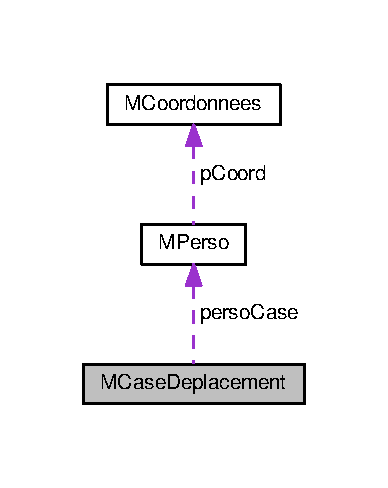
\includegraphics[width=186pt]{structMCaseDeplacement__coll__graph}
\end{center}
\end{figure}
\subsection*{Attributs publics}
\begin{DoxyCompactItemize}
\item 
\hyperlink{caseDeplacement_8h_af9a4f51a2aa1485342c48472a9124d83}{env} \hyperlink{structMCaseDeplacement_a39fe908c7afa0eb210c77d12bb96a99e}{env\+Case}
\item 
struct \hyperlink{structMPerso}{M\+Perso} $\ast$ \hyperlink{structMCaseDeplacement_a4c1dce63d49728610cc667865d0661e2}{perso\+Case}
\item 
unsigned short \hyperlink{structMCaseDeplacement_a3507b4494325ec01693f9034eed8f681}{champ\+Zombies} \mbox{[}250\mbox{]}
\item 
unsigned short \hyperlink{structMCaseDeplacement_a992e7ffc50e45a8fb49a982dcc392aa8}{champ\+Citoyens} \mbox{[}250\mbox{]}
\item 
unsigned short \hyperlink{structMCaseDeplacement_a98792df104a1bbab569aa9d0a86af554}{champ\+Policiers} \mbox{[}250\mbox{]}
\end{DoxyCompactItemize}


\subsection{Description détaillée}
Structure definissant les cases de déplacement (champs d\textquotesingle{}influences et environement) 

\subsection{Documentation des données membres}
\index{M\+Case\+Deplacement@{M\+Case\+Deplacement}!champ\+Citoyens@{champ\+Citoyens}}
\index{champ\+Citoyens@{champ\+Citoyens}!M\+Case\+Deplacement@{M\+Case\+Deplacement}}
\subsubsection[{\texorpdfstring{champ\+Citoyens}{champCitoyens}}]{\setlength{\rightskip}{0pt plus 5cm}M\+Case\+Deplacement\+::champ\+Citoyens\mbox{[}250\mbox{]}}\hypertarget{structMCaseDeplacement_a992e7ffc50e45a8fb49a982dcc392aa8}{}\label{structMCaseDeplacement_a992e7ffc50e45a8fb49a982dcc392aa8}
Champs des citoyens présents sur le terrain en cette case \index{M\+Case\+Deplacement@{M\+Case\+Deplacement}!champ\+Policiers@{champ\+Policiers}}
\index{champ\+Policiers@{champ\+Policiers}!M\+Case\+Deplacement@{M\+Case\+Deplacement}}
\subsubsection[{\texorpdfstring{champ\+Policiers}{champPoliciers}}]{\setlength{\rightskip}{0pt plus 5cm}M\+Case\+Deplacement\+::champ\+Policiers\mbox{[}250\mbox{]}}\hypertarget{structMCaseDeplacement_a98792df104a1bbab569aa9d0a86af554}{}\label{structMCaseDeplacement_a98792df104a1bbab569aa9d0a86af554}
Champs des policiers présents sur le terrain en cette case \index{M\+Case\+Deplacement@{M\+Case\+Deplacement}!champ\+Zombies@{champ\+Zombies}}
\index{champ\+Zombies@{champ\+Zombies}!M\+Case\+Deplacement@{M\+Case\+Deplacement}}
\subsubsection[{\texorpdfstring{champ\+Zombies}{champZombies}}]{\setlength{\rightskip}{0pt plus 5cm}M\+Case\+Deplacement\+::champ\+Zombies\mbox{[}250\mbox{]}}\hypertarget{structMCaseDeplacement_a3507b4494325ec01693f9034eed8f681}{}\label{structMCaseDeplacement_a3507b4494325ec01693f9034eed8f681}
Champs des zombies présents sur le terrain en cette case \index{M\+Case\+Deplacement@{M\+Case\+Deplacement}!env\+Case@{env\+Case}}
\index{env\+Case@{env\+Case}!M\+Case\+Deplacement@{M\+Case\+Deplacement}}
\subsubsection[{\texorpdfstring{env\+Case}{envCase}}]{\setlength{\rightskip}{0pt plus 5cm}M\+Case\+Deplacement\+::env\+Case}\hypertarget{structMCaseDeplacement_a39fe908c7afa0eb210c77d12bb96a99e}{}\label{structMCaseDeplacement_a39fe908c7afa0eb210c77d12bb96a99e}
Type de case, mur ou sol \index{M\+Case\+Deplacement@{M\+Case\+Deplacement}!perso\+Case@{perso\+Case}}
\index{perso\+Case@{perso\+Case}!M\+Case\+Deplacement@{M\+Case\+Deplacement}}
\subsubsection[{\texorpdfstring{perso\+Case}{persoCase}}]{\setlength{\rightskip}{0pt plus 5cm}M\+Case\+Deplacement\+::perso\+Case}\hypertarget{structMCaseDeplacement_a4c1dce63d49728610cc667865d0661e2}{}\label{structMCaseDeplacement_a4c1dce63d49728610cc667865d0661e2}
Pointeur vers un eventuel personnage sur la case 

La documentation de cette structure a été générée à partir du fichier suivant \+:\begin{DoxyCompactItemize}
\item 
src/\hyperlink{caseDeplacement_8h}{case\+Deplacement.\+h}\end{DoxyCompactItemize}

\hypertarget{structMCoordonnees}{}\section{Référence de la structure M\+Coordonnees}
\label{structMCoordonnees}\index{M\+Coordonnees@{M\+Coordonnees}}


Structure definissant des coordonnees en deux dimension (pour des entitées)  




{\ttfamily \#include $<$coordonnees.\+h$>$}

\subsection*{Attributs publics}
\begin{DoxyCompactItemize}
\item 
int \hyperlink{structMCoordonnees_acbeda4a908264671eff2ea4aaacc68cc}{x\+Coord}
\item 
int \hyperlink{structMCoordonnees_a161feac6dbc750cf54906e9938e0f97f}{y\+Coord}
\end{DoxyCompactItemize}


\subsection{Description détaillée}
Structure definissant des coordonnees en deux dimension (pour des entitées) 

\subsection{Documentation des données membres}
\index{M\+Coordonnees@{M\+Coordonnees}!x\+Coord@{x\+Coord}}
\index{x\+Coord@{x\+Coord}!M\+Coordonnees@{M\+Coordonnees}}
\subsubsection[{\texorpdfstring{x\+Coord}{xCoord}}]{\setlength{\rightskip}{0pt plus 5cm}M\+Coordonnees\+::x\+Coord}\hypertarget{structMCoordonnees_acbeda4a908264671eff2ea4aaacc68cc}{}\label{structMCoordonnees_acbeda4a908264671eff2ea4aaacc68cc}
Position sur l\textquotesingle{}axe des X \index{M\+Coordonnees@{M\+Coordonnees}!y\+Coord@{y\+Coord}}
\index{y\+Coord@{y\+Coord}!M\+Coordonnees@{M\+Coordonnees}}
\subsubsection[{\texorpdfstring{y\+Coord}{yCoord}}]{\setlength{\rightskip}{0pt plus 5cm}M\+Coordonnees\+::y\+Coord}\hypertarget{structMCoordonnees_a161feac6dbc750cf54906e9938e0f97f}{}\label{structMCoordonnees_a161feac6dbc750cf54906e9938e0f97f}
Position sur l\textquotesingle{}axe des Y 

La documentation de cette structure a été générée à partir du fichier suivant \+:\begin{DoxyCompactItemize}
\item 
src/\hyperlink{coordonnees_8h}{coordonnees.\+h}\end{DoxyCompactItemize}

\hypertarget{structMPerso}{}\section{Référence de la structure M\+Perso}
\label{structMPerso}\index{M\+Perso@{M\+Perso}}


Structure definissant un personnage et ses attributs.  




{\ttfamily \#include $<$personnage.\+h$>$}



Graphe de collaboration de M\+Perso\+:\nopagebreak
\begin{figure}[H]
\begin{center}
\leavevmode
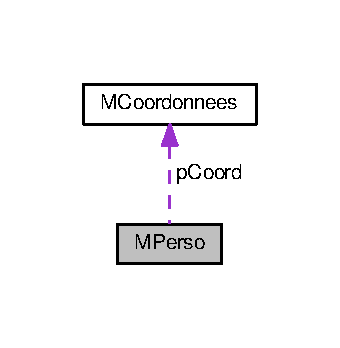
\includegraphics[width=163pt]{structMPerso__coll__graph}
\end{center}
\end{figure}
\subsection*{Attributs publics}
\begin{DoxyCompactItemize}
\item 
int \hyperlink{structMPerso_af6a4c47de69856669b2f1810d4c870e7}{id}
\item 
\hyperlink{coordonnees_8h_a79929cdfee7bd985a5e4e25276bb3ba9}{Coordonnees} $\ast$ \hyperlink{structMPerso_aa1a6adaf74d536a913f11ed632ddb8d1}{p\+Coord}
\item 
enum \hyperlink{personnage_8h_a3f6a2951aa3d5d428dd6d61e74db0d75}{type\+Perso} \hyperlink{structMPerso_a476ff327af93f97f1ae6408e2ebc1986}{type}
\end{DoxyCompactItemize}


\subsection{Description détaillée}
Structure definissant un personnage et ses attributs. 

\subsection{Documentation des données membres}
\index{M\+Perso@{M\+Perso}!id@{id}}
\index{id@{id}!M\+Perso@{M\+Perso}}
\subsubsection[{\texorpdfstring{id}{id}}]{\setlength{\rightskip}{0pt plus 5cm}M\+Perso\+::id}\hypertarget{structMPerso_af6a4c47de69856669b2f1810d4c870e7}{}\label{structMPerso_af6a4c47de69856669b2f1810d4c870e7}
id D\textquotesingle{}un personnage servant à l\textquotesingle{}identifier \index{M\+Perso@{M\+Perso}!p\+Coord@{p\+Coord}}
\index{p\+Coord@{p\+Coord}!M\+Perso@{M\+Perso}}
\subsubsection[{\texorpdfstring{p\+Coord}{pCoord}}]{\setlength{\rightskip}{0pt plus 5cm}{\bf Coordonnees}$\ast$ M\+Perso\+::p\+Coord}\hypertarget{structMPerso_aa1a6adaf74d536a913f11ed632ddb8d1}{}\label{structMPerso_aa1a6adaf74d536a913f11ed632ddb8d1}
\index{M\+Perso@{M\+Perso}!type@{type}}
\index{type@{type}!M\+Perso@{M\+Perso}}
\subsubsection[{\texorpdfstring{type}{type}}]{\setlength{\rightskip}{0pt plus 5cm}M\+Perso\+::type}\hypertarget{structMPerso_a476ff327af93f97f1ae6408e2ebc1986}{}\label{structMPerso_a476ff327af93f97f1ae6408e2ebc1986}
Type du personnage zombie,citoyen ou humain 

La documentation de cette structure a été générée à partir du fichier suivant \+:\begin{DoxyCompactItemize}
\item 
src/\hyperlink{personnage_8h}{personnage.\+h}\end{DoxyCompactItemize}

\hypertarget{structMSimulation}{}\section{Référence de la structure M\+Simulation}
\label{structMSimulation}\index{M\+Simulation@{M\+Simulation}}


Structure definissant une simulation et ses attributs.  




{\ttfamily \#include $<$simulation.\+h$>$}



Graphe de collaboration de M\+Simulation\+:
\nopagebreak
\begin{figure}[H]
\begin{center}
\leavevmode
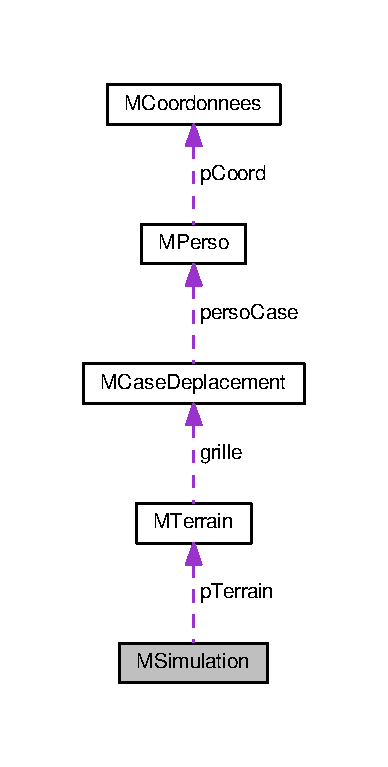
\includegraphics[width=186pt]{structMSimulation__coll__graph}
\end{center}
\end{figure}
\subsection*{Attributs publics}
\begin{DoxyCompactItemize}
\item 
\hyperlink{terrain_8h_a11bbfdc6f8212f3246205cc0e7134136}{Terrain} $\ast$ \hyperlink{structMSimulation_aefc18c24eb2ab2f1224ff2063114122b}{p\+Terrain}
\item 
int \hyperlink{structMSimulation_a2be6307fb9eeb91c0292e363e61e0c1a}{nb\+Zombies}
\item 
int \hyperlink{structMSimulation_a9bbc6c7c49600206282cfa0e906bd502}{nb\+Citoyens}
\item 
int \hyperlink{structMSimulation_a36feaca3afcb2dca6023254639ce545c}{nb\+Policiers}
\item 
G\+Array $\ast$ \hyperlink{structMSimulation_ab18a020f5a29032678796540fdb981cc}{zombies}
\item 
G\+Array $\ast$ \hyperlink{structMSimulation_a3468065bed2a665bd316109c5a3b6480}{citoyens}
\item 
G\+Array $\ast$ \hyperlink{structMSimulation_a8281fb3df339f2006ce172e9de7d6910}{policiers}
\end{DoxyCompactItemize}


\subsection{Description détaillée}
Structure definissant une simulation et ses attributs. 

\subsection{Documentation des données membres}
\index{M\+Simulation@{M\+Simulation}!citoyens@{citoyens}}
\index{citoyens@{citoyens}!M\+Simulation@{M\+Simulation}}
\subsubsection[{\texorpdfstring{citoyens}{citoyens}}]{\setlength{\rightskip}{0pt plus 5cm}M\+Simulation\+::citoyens}\hypertarget{structMSimulation_a3468065bed2a665bd316109c5a3b6480}{}\label{structMSimulation_a3468065bed2a665bd316109c5a3b6480}
Tableau des citoyens \index{M\+Simulation@{M\+Simulation}!nb\+Citoyens@{nb\+Citoyens}}
\index{nb\+Citoyens@{nb\+Citoyens}!M\+Simulation@{M\+Simulation}}
\subsubsection[{\texorpdfstring{nb\+Citoyens}{nbCitoyens}}]{\setlength{\rightskip}{0pt plus 5cm}M\+Simulation\+::nb\+Citoyens}\hypertarget{structMSimulation_a9bbc6c7c49600206282cfa0e906bd502}{}\label{structMSimulation_a9bbc6c7c49600206282cfa0e906bd502}
Nombre de citoyens \index{M\+Simulation@{M\+Simulation}!nb\+Policiers@{nb\+Policiers}}
\index{nb\+Policiers@{nb\+Policiers}!M\+Simulation@{M\+Simulation}}
\subsubsection[{\texorpdfstring{nb\+Policiers}{nbPoliciers}}]{\setlength{\rightskip}{0pt plus 5cm}M\+Simulation\+::nb\+Policiers}\hypertarget{structMSimulation_a36feaca3afcb2dca6023254639ce545c}{}\label{structMSimulation_a36feaca3afcb2dca6023254639ce545c}
Nombre de policiers \index{M\+Simulation@{M\+Simulation}!nb\+Zombies@{nb\+Zombies}}
\index{nb\+Zombies@{nb\+Zombies}!M\+Simulation@{M\+Simulation}}
\subsubsection[{\texorpdfstring{nb\+Zombies}{nbZombies}}]{\setlength{\rightskip}{0pt plus 5cm}M\+Simulation\+::nb\+Zombies}\hypertarget{structMSimulation_a2be6307fb9eeb91c0292e363e61e0c1a}{}\label{structMSimulation_a2be6307fb9eeb91c0292e363e61e0c1a}
Nombres de Zombies \index{M\+Simulation@{M\+Simulation}!policiers@{policiers}}
\index{policiers@{policiers}!M\+Simulation@{M\+Simulation}}
\subsubsection[{\texorpdfstring{policiers}{policiers}}]{\setlength{\rightskip}{0pt plus 5cm}M\+Simulation\+::policiers}\hypertarget{structMSimulation_a8281fb3df339f2006ce172e9de7d6910}{}\label{structMSimulation_a8281fb3df339f2006ce172e9de7d6910}
Tableau des policiers \index{M\+Simulation@{M\+Simulation}!p\+Terrain@{p\+Terrain}}
\index{p\+Terrain@{p\+Terrain}!M\+Simulation@{M\+Simulation}}
\subsubsection[{\texorpdfstring{p\+Terrain}{pTerrain}}]{\setlength{\rightskip}{0pt plus 5cm}M\+Simulation\+::p\+Terrain}\hypertarget{structMSimulation_aefc18c24eb2ab2f1224ff2063114122b}{}\label{structMSimulation_aefc18c24eb2ab2f1224ff2063114122b}
Pointeur vers un terrain associé à la simulation \index{M\+Simulation@{M\+Simulation}!zombies@{zombies}}
\index{zombies@{zombies}!M\+Simulation@{M\+Simulation}}
\subsubsection[{\texorpdfstring{zombies}{zombies}}]{\setlength{\rightskip}{0pt plus 5cm}M\+Simulation\+::zombies}\hypertarget{structMSimulation_ab18a020f5a29032678796540fdb981cc}{}\label{structMSimulation_ab18a020f5a29032678796540fdb981cc}
Tableau des zombies 

La documentation de cette structure a été générée à partir du fichier suivant \+:\begin{DoxyCompactItemize}
\item 
src/\hyperlink{simulation_8h}{simulation.\+h}\end{DoxyCompactItemize}

\hypertarget{structMTerrain}{}\section{Référence de la structure M\+Terrain}
\label{structMTerrain}\index{M\+Terrain@{M\+Terrain}}


Structure definissant un terrain et ses dimensions.  




{\ttfamily \#include $<$terrain.\+h$>$}



Graphe de collaboration de M\+Terrain\+:\nopagebreak
\begin{figure}[H]
\begin{center}
\leavevmode
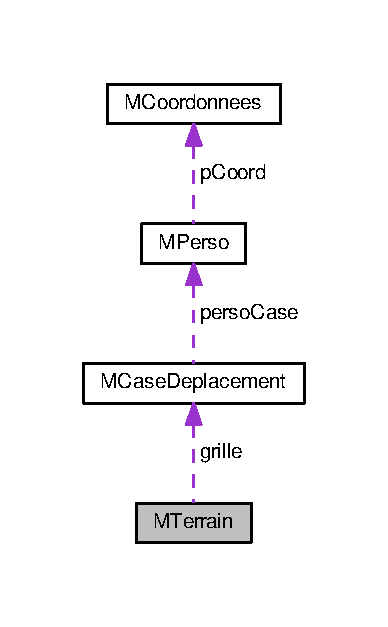
\includegraphics[width=186pt]{structMTerrain__coll__graph}
\end{center}
\end{figure}
\subsection*{Attributs publics}
\begin{DoxyCompactItemize}
\item 
int \hyperlink{structMTerrain_ae6f66d485448ae93c427e0586d6b12aa}{dimX}
\item 
int \hyperlink{structMTerrain_a638d309791fdf84d0267d75702bbab50}{dimY}
\item 
char \hyperlink{structMTerrain_a948d5d38016eed56187a94028e34f5e4}{nom\+Terrain} \mbox{[}\hyperlink{terrain_8h_a5f41c70ea486e890717560da2605f309}{M\+A\+X\+\_\+\+C\+H\+A\+R\+\_\+\+N\+O\+M\+\_\+\+T\+E\+R\+R\+A\+IN}\mbox{]}
\item 
\hyperlink{caseDeplacement_8h_aeab4f22b99f0db8b549dab4e46e3ead4}{case\+Deplacement} $\ast$ \hyperlink{structMTerrain_a392b4ed453bab400087d0bda7d452877}{grille}
\end{DoxyCompactItemize}


\subsection{Description détaillée}
Structure definissant un terrain et ses dimensions. 

\subsection{Documentation des données membres}
\index{M\+Terrain@{M\+Terrain}!dimX@{dimX}}
\index{dimX@{dimX}!M\+Terrain@{M\+Terrain}}
\subsubsection[{\texorpdfstring{dimX}{dimX}}]{\setlength{\rightskip}{0pt plus 5cm}M\+Terrain\+::dimX}\hypertarget{structMTerrain_ae6f66d485448ae93c427e0586d6b12aa}{}\label{structMTerrain_ae6f66d485448ae93c427e0586d6b12aa}
Largeur du terrain \index{M\+Terrain@{M\+Terrain}!dimY@{dimY}}
\index{dimY@{dimY}!M\+Terrain@{M\+Terrain}}
\subsubsection[{\texorpdfstring{dimY}{dimY}}]{\setlength{\rightskip}{0pt plus 5cm}M\+Terrain\+::dimY}\hypertarget{structMTerrain_a638d309791fdf84d0267d75702bbab50}{}\label{structMTerrain_a638d309791fdf84d0267d75702bbab50}
Hauteur du terrain \index{M\+Terrain@{M\+Terrain}!grille@{grille}}
\index{grille@{grille}!M\+Terrain@{M\+Terrain}}
\subsubsection[{\texorpdfstring{grille}{grille}}]{\setlength{\rightskip}{0pt plus 5cm}M\+Terrain\+::grille}\hypertarget{structMTerrain_a392b4ed453bab400087d0bda7d452877}{}\label{structMTerrain_a392b4ed453bab400087d0bda7d452877}
Grille a deux dimension de carractere definisant la grille du terrain (sol / mur) \index{M\+Terrain@{M\+Terrain}!nom\+Terrain@{nom\+Terrain}}
\index{nom\+Terrain@{nom\+Terrain}!M\+Terrain@{M\+Terrain}}
\subsubsection[{\texorpdfstring{nom\+Terrain}{nomTerrain}}]{\setlength{\rightskip}{0pt plus 5cm}M\+Terrain\+::nom\+Terrain}\hypertarget{structMTerrain_a948d5d38016eed56187a94028e34f5e4}{}\label{structMTerrain_a948d5d38016eed56187a94028e34f5e4}
Nom du Terrain en chaine de carractere limité a 101 carracteres 

La documentation de cette structure a été générée à partir du fichier suivant \+:\begin{DoxyCompactItemize}
\item 
src/\hyperlink{terrain_8h}{terrain.\+h}\end{DoxyCompactItemize}

\chapter{Documentation des fichiers}
\hypertarget{caseDeplacement_8c}{}\section{Référence du fichier src/case\+Deplacement.c}
\label{caseDeplacement_8c}\index{src/case\+Deplacement.\+c@{src/case\+Deplacement.\+c}}
{\ttfamily \#include \char`\"{}case\+Deplacement.\+h\char`\"{}}\\*
Graphe des dépendances par inclusion de case\+Deplacement.\+c\+:\nopagebreak
\begin{figure}[H]
\begin{center}
\leavevmode
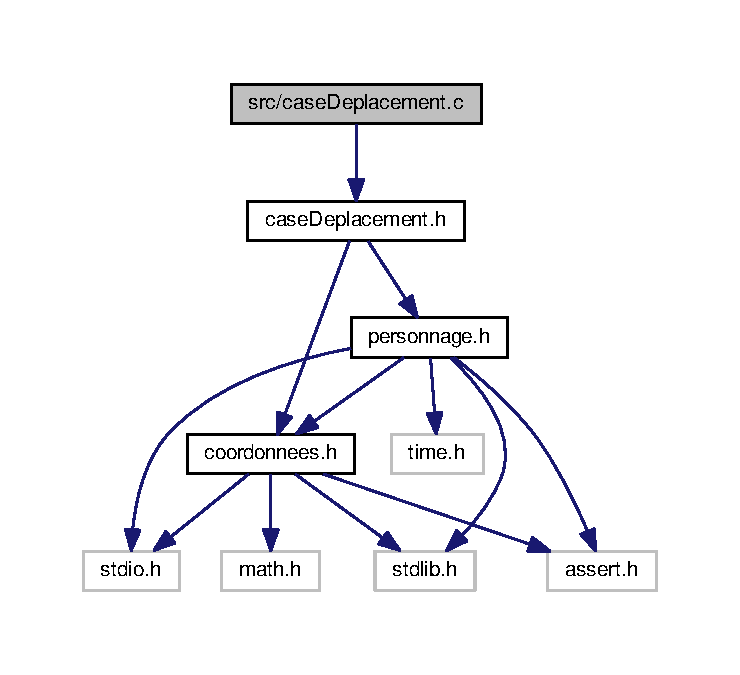
\includegraphics[width=350pt]{caseDeplacement_8c__incl}
\end{center}
\end{figure}
\subsection*{Fonctions}
\begin{DoxyCompactItemize}
\item 
enum \hyperlink{caseDeplacement_8h_af9a4f51a2aa1485342c48472a9124d83}{env} \hyperlink{caseDeplacement_8c_a3b6655cf83e6bc1c84ef1dd02f204e0b}{get\+Env\+Case} (\hyperlink{caseDeplacement_8h_aeab4f22b99f0db8b549dab4e46e3ead4}{case\+Deplacement} $\ast$p\+Case\+Dep)
\begin{DoxyCompactList}\small\item\em Recupère le type de case d\textquotesingle{}une case de deplacement. \end{DoxyCompactList}\item 
\hyperlink{personnage_8h_abd5c92a453bbf273f753b3f5b99da9e7}{Perso} $\ast$ \hyperlink{caseDeplacement_8c_a6b8c143eea4a9242b0f59a634c2f81b0}{get\+Perso\+Case} (\hyperlink{caseDeplacement_8h_aeab4f22b99f0db8b549dab4e46e3ead4}{case\+Deplacement} $\ast$p\+Case\+Dep)
\begin{DoxyCompactList}\small\item\em Recupère le personnage sur la case de déplacement. \end{DoxyCompactList}\item 
void \hyperlink{caseDeplacement_8c_abb53fe7469ac0c9441d4bb3959365a42}{set\+Env\+Case} (\hyperlink{caseDeplacement_8h_aeab4f22b99f0db8b549dab4e46e3ead4}{case\+Deplacement} $\ast$p\+Case\+Dep, \hyperlink{caseDeplacement_8h_af9a4f51a2aa1485342c48472a9124d83}{env} valeur\+Env)
\begin{DoxyCompactList}\small\item\em Modifie le type de case d\textquotesingle{}une case de deplacement. \end{DoxyCompactList}\item 
void \hyperlink{caseDeplacement_8c_a2be2ab36936e9a5cb9fd2948353c7b12}{set\+Perso\+Case} (\hyperlink{caseDeplacement_8h_aeab4f22b99f0db8b549dab4e46e3ead4}{case\+Deplacement} $\ast$p\+Case\+Dep, \hyperlink{personnage_8h_abd5c92a453bbf273f753b3f5b99da9e7}{Perso} $\ast$p\+Perso)
\begin{DoxyCompactList}\small\item\em Modifie le personnage sur la case de déplacement. \end{DoxyCompactList}\item 
unsigned short \hyperlink{caseDeplacement_8c_a271e610d4e5a86cabe14f2f9ae463442}{get\+Champ} (enum \hyperlink{personnage_8h_a3f6a2951aa3d5d428dd6d61e74db0d75}{type\+Perso} type, int id\+Perso, \hyperlink{caseDeplacement_8h_aeab4f22b99f0db8b549dab4e46e3ead4}{case\+Deplacement} $\ast$p\+Case\+Dep)
\begin{DoxyCompactList}\small\item\em Récupère la valeur du champ du perso défini par son type et son id sur une case. \end{DoxyCompactList}\item 
void \hyperlink{caseDeplacement_8c_ad8f191fd46363452d5e40a19326fefc5}{set\+Champ} (unsigned short intensite, enum \hyperlink{personnage_8h_a3f6a2951aa3d5d428dd6d61e74db0d75}{type\+Perso} type, int id\+Perso, \hyperlink{caseDeplacement_8h_aeab4f22b99f0db8b549dab4e46e3ead4}{case\+Deplacement} $\ast$case\+Dep)
\begin{DoxyCompactList}\small\item\em Définit la valeur du champ du perso défini par son type et son id sur une case. \end{DoxyCompactList}\item 
\hyperlink{caseDeplacement_8h_aeab4f22b99f0db8b549dab4e46e3ead4}{case\+Deplacement} $\ast$ \hyperlink{caseDeplacement_8c_a7ef31ff562e58ed644b58bc85dac2534}{init\+Case} (enum \hyperlink{caseDeplacement_8h_af9a4f51a2aa1485342c48472a9124d83}{env} env\+Case, \hyperlink{personnage_8h_abd5c92a453bbf273f753b3f5b99da9e7}{Perso} $\ast$p\+Perso)
\begin{DoxyCompactList}\small\item\em Crée et initialise une case de deplacement avec un type de case et un personnage dessus. \end{DoxyCompactList}\item 
void \hyperlink{caseDeplacement_8c_ae8dd0ca56ce6c60c91d32a739e9d471d}{testament\+Case} (\hyperlink{caseDeplacement_8h_aeab4f22b99f0db8b549dab4e46e3ead4}{case\+Deplacement} $\ast$case\+Dep)
\end{DoxyCompactItemize}


\subsection{Documentation des fonctions}
\index{case\+Deplacement.\+c@{case\+Deplacement.\+c}!get\+Champ@{get\+Champ}}
\index{get\+Champ@{get\+Champ}!case\+Deplacement.\+c@{case\+Deplacement.\+c}}
\subsubsection[{\texorpdfstring{get\+Champ(enum type\+Perso type, int id\+Perso, case\+Deplacement $\ast$p\+Case\+Dep)}{getChamp(enum typePerso type, int idPerso, caseDeplacement *pCaseDep)}}]{\setlength{\rightskip}{0pt plus 5cm}unsigned short get\+Champ (
\begin{DoxyParamCaption}
\item[{enum {\bf type\+Perso}}]{type, }
\item[{int}]{id\+Perso, }
\item[{{\bf case\+Deplacement} $\ast$}]{p\+Case\+Dep}
\end{DoxyParamCaption}
)}\hypertarget{caseDeplacement_8c_a271e610d4e5a86cabe14f2f9ae463442}{}\label{caseDeplacement_8c_a271e610d4e5a86cabe14f2f9ae463442}


Récupère la valeur du champ du perso défini par son type et son id sur une case. 


\begin{DoxyParams}{Paramètres}
{\em type} & Type du perso (Z\+O\+M\+B\+IE, P\+O\+L\+I\+C\+I\+ER, C\+I\+T\+O\+Y\+EN) \\
\hline
{\em id\+Perso} & Id du perso dont on veut connaitre le champ \\
\hline
{\em p\+Case\+Dep} & Pointeur vers la case a detruire et liberer \\
\hline
\end{DoxyParams}
\index{case\+Deplacement.\+c@{case\+Deplacement.\+c}!get\+Env\+Case@{get\+Env\+Case}}
\index{get\+Env\+Case@{get\+Env\+Case}!case\+Deplacement.\+c@{case\+Deplacement.\+c}}
\subsubsection[{\texorpdfstring{get\+Env\+Case(case\+Deplacement $\ast$p\+Case\+Dep)}{getEnvCase(caseDeplacement *pCaseDep)}}]{\setlength{\rightskip}{0pt plus 5cm}enum {\bf env} get\+Env\+Case (
\begin{DoxyParamCaption}
\item[{{\bf case\+Deplacement} $\ast$}]{p\+Case\+Dep}
\end{DoxyParamCaption}
)}\hypertarget{caseDeplacement_8c_a3b6655cf83e6bc1c84ef1dd02f204e0b}{}\label{caseDeplacement_8c_a3b6655cf83e6bc1c84ef1dd02f204e0b}


Recupère le type de case d\textquotesingle{}une case de deplacement. 


\begin{DoxyParams}{Paramètres}
{\em p\+Case\+Dep} & Pointeur sur la case de déplacement à étudier \\
\hline
\end{DoxyParams}
\begin{DoxyReturn}{Renvoie}
Le type de case 
\end{DoxyReturn}
\index{case\+Deplacement.\+c@{case\+Deplacement.\+c}!get\+Perso\+Case@{get\+Perso\+Case}}
\index{get\+Perso\+Case@{get\+Perso\+Case}!case\+Deplacement.\+c@{case\+Deplacement.\+c}}
\subsubsection[{\texorpdfstring{get\+Perso\+Case(case\+Deplacement $\ast$p\+Case\+Dep)}{getPersoCase(caseDeplacement *pCaseDep)}}]{\setlength{\rightskip}{0pt plus 5cm}{\bf Perso}$\ast$ get\+Perso\+Case (
\begin{DoxyParamCaption}
\item[{{\bf case\+Deplacement} $\ast$}]{p\+Case\+Dep}
\end{DoxyParamCaption}
)}\hypertarget{caseDeplacement_8c_a6b8c143eea4a9242b0f59a634c2f81b0}{}\label{caseDeplacement_8c_a6b8c143eea4a9242b0f59a634c2f81b0}


Recupère le personnage sur la case de déplacement. 


\begin{DoxyParams}{Paramètres}
{\em p\+Case\+Dep} & Pointeur sur la case de déplacement à étudier \\
\hline
\end{DoxyParams}
\begin{DoxyReturn}{Renvoie}
Pointeur vers le personnage sur la case de déplacement 
\end{DoxyReturn}
\index{case\+Deplacement.\+c@{case\+Deplacement.\+c}!init\+Case@{init\+Case}}
\index{init\+Case@{init\+Case}!case\+Deplacement.\+c@{case\+Deplacement.\+c}}
\subsubsection[{\texorpdfstring{init\+Case(enum env env\+Case, Perso $\ast$p\+Perso)}{initCase(enum env envCase, Perso *pPerso)}}]{\setlength{\rightskip}{0pt plus 5cm}{\bf case\+Deplacement}$\ast$ init\+Case (
\begin{DoxyParamCaption}
\item[{enum {\bf env}}]{env\+Case, }
\item[{{\bf Perso} $\ast$}]{p\+Perso}
\end{DoxyParamCaption}
)}\hypertarget{caseDeplacement_8c_a7ef31ff562e58ed644b58bc85dac2534}{}\label{caseDeplacement_8c_a7ef31ff562e58ed644b58bc85dac2534}


Crée et initialise une case de deplacement avec un type de case et un personnage dessus. 


\begin{DoxyParams}{Paramètres}
{\em env\+Case} & Type de case \\
\hline
{\em p\+Perso} & Pointeur vers un personnage \\
\hline
\end{DoxyParams}
\begin{DoxyReturn}{Renvoie}
Pointeur vers cette case de deplacement 
\end{DoxyReturn}
\index{case\+Deplacement.\+c@{case\+Deplacement.\+c}!set\+Champ@{set\+Champ}}
\index{set\+Champ@{set\+Champ}!case\+Deplacement.\+c@{case\+Deplacement.\+c}}
\subsubsection[{\texorpdfstring{set\+Champ(unsigned short intensite, enum type\+Perso type, int id\+Perso, case\+Deplacement $\ast$case\+Dep)}{setChamp(unsigned short intensite, enum typePerso type, int idPerso, caseDeplacement *caseDep)}}]{\setlength{\rightskip}{0pt plus 5cm}void set\+Champ (
\begin{DoxyParamCaption}
\item[{unsigned short}]{intensite, }
\item[{enum {\bf type\+Perso}}]{type, }
\item[{int}]{id\+Perso, }
\item[{{\bf case\+Deplacement} $\ast$}]{p\+Case\+Dep}
\end{DoxyParamCaption}
)}\hypertarget{caseDeplacement_8c_ad8f191fd46363452d5e40a19326fefc5}{}\label{caseDeplacement_8c_ad8f191fd46363452d5e40a19326fefc5}


Définit la valeur du champ du perso défini par son type et son id sur une case. 


\begin{DoxyParams}{Paramètres}
{\em type} & Type du perso (Z\+O\+M\+B\+IE, P\+O\+L\+I\+C\+I\+ER, C\+I\+T\+O\+Y\+EN) \\
\hline
{\em id\+Perso} & Id du perso dont on veut connaitre le champ \\
\hline
{\em p\+Case\+Dep} & Pointeur vers la case a detruire et liberer \\
\hline
\end{DoxyParams}
\index{case\+Deplacement.\+c@{case\+Deplacement.\+c}!set\+Env\+Case@{set\+Env\+Case}}
\index{set\+Env\+Case@{set\+Env\+Case}!case\+Deplacement.\+c@{case\+Deplacement.\+c}}
\subsubsection[{\texorpdfstring{set\+Env\+Case(case\+Deplacement $\ast$p\+Case\+Dep, env valeur\+Env)}{setEnvCase(caseDeplacement *pCaseDep, env valeurEnv)}}]{\setlength{\rightskip}{0pt plus 5cm}void set\+Env\+Case (
\begin{DoxyParamCaption}
\item[{{\bf case\+Deplacement} $\ast$}]{p\+Case\+Dep, }
\item[{enum {\bf env}}]{valeur\+Env}
\end{DoxyParamCaption}
)}\hypertarget{caseDeplacement_8c_abb53fe7469ac0c9441d4bb3959365a42}{}\label{caseDeplacement_8c_abb53fe7469ac0c9441d4bb3959365a42}


Modifie le type de case d\textquotesingle{}une case de deplacement. 


\begin{DoxyParams}{Paramètres}
{\em p\+Case\+Dep} & Pointeur sur la case de déplacement à étudier \\
\hline
{\em valeur\+Env} & Le type de case \\
\hline
\end{DoxyParams}
\index{case\+Deplacement.\+c@{case\+Deplacement.\+c}!set\+Perso\+Case@{set\+Perso\+Case}}
\index{set\+Perso\+Case@{set\+Perso\+Case}!case\+Deplacement.\+c@{case\+Deplacement.\+c}}
\subsubsection[{\texorpdfstring{set\+Perso\+Case(case\+Deplacement $\ast$p\+Case\+Dep, Perso $\ast$p\+Perso)}{setPersoCase(caseDeplacement *pCaseDep, Perso *pPerso)}}]{\setlength{\rightskip}{0pt plus 5cm}void set\+Perso\+Case (
\begin{DoxyParamCaption}
\item[{{\bf case\+Deplacement} $\ast$}]{p\+Case\+Dep, }
\item[{{\bf Perso} $\ast$}]{p\+Perso}
\end{DoxyParamCaption}
)}\hypertarget{caseDeplacement_8c_a2be2ab36936e9a5cb9fd2948353c7b12}{}\label{caseDeplacement_8c_a2be2ab36936e9a5cb9fd2948353c7b12}


Modifie le personnage sur la case de déplacement. 


\begin{DoxyParams}{Paramètres}
{\em p\+Case\+Dep} & Pointeur sur la case de déplacement à étudier \\
\hline
{\em p\+Perso} & Pointeur vers le personnage a mettre sur la case de déplacement \\
\hline
\end{DoxyParams}
\index{case\+Deplacement.\+c@{case\+Deplacement.\+c}!testament\+Case@{testament\+Case}}
\index{testament\+Case@{testament\+Case}!case\+Deplacement.\+c@{case\+Deplacement.\+c}}
\subsubsection[{\texorpdfstring{testament\+Case(case\+Deplacement $\ast$case\+Dep)}{testamentCase(caseDeplacement *caseDep)}}]{\setlength{\rightskip}{0pt plus 5cm}void testament\+Case (
\begin{DoxyParamCaption}
\item[{{\bf case\+Deplacement} $\ast$}]{case\+Dep}
\end{DoxyParamCaption}
)}\hypertarget{caseDeplacement_8c_ae8dd0ca56ce6c60c91d32a739e9d471d}{}\label{caseDeplacement_8c_ae8dd0ca56ce6c60c91d32a739e9d471d}

\hypertarget{caseDeplacement_8h}{}\section{Référence du fichier src/case\+Deplacement.h}
\label{caseDeplacement_8h}\index{src/case\+Deplacement.\+h@{src/case\+Deplacement.\+h}}


Définit une case sur lesquels les personnages vont pouvoir se déplacer.  


{\ttfamily \#include \char`\"{}coordonnees.\+h\char`\"{}}\\*
{\ttfamily \#include \char`\"{}personnage.\+h\char`\"{}}\\*
Graphe des dépendances par inclusion de case\+Deplacement.\+h\+:
\nopagebreak
\begin{figure}[H]
\begin{center}
\leavevmode
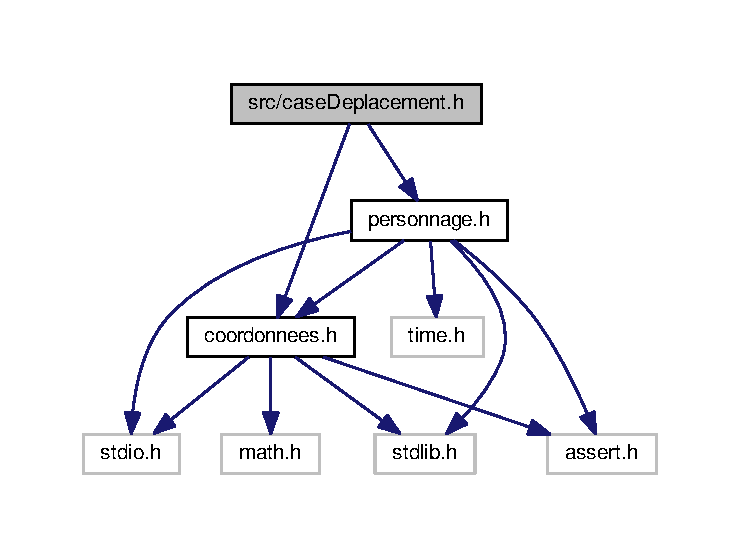
\includegraphics[width=350pt]{caseDeplacement_8h__incl}
\end{center}
\end{figure}
Ce graphe montre quels fichiers incluent directement ou indirectement ce fichier \+:
\nopagebreak
\begin{figure}[H]
\begin{center}
\leavevmode
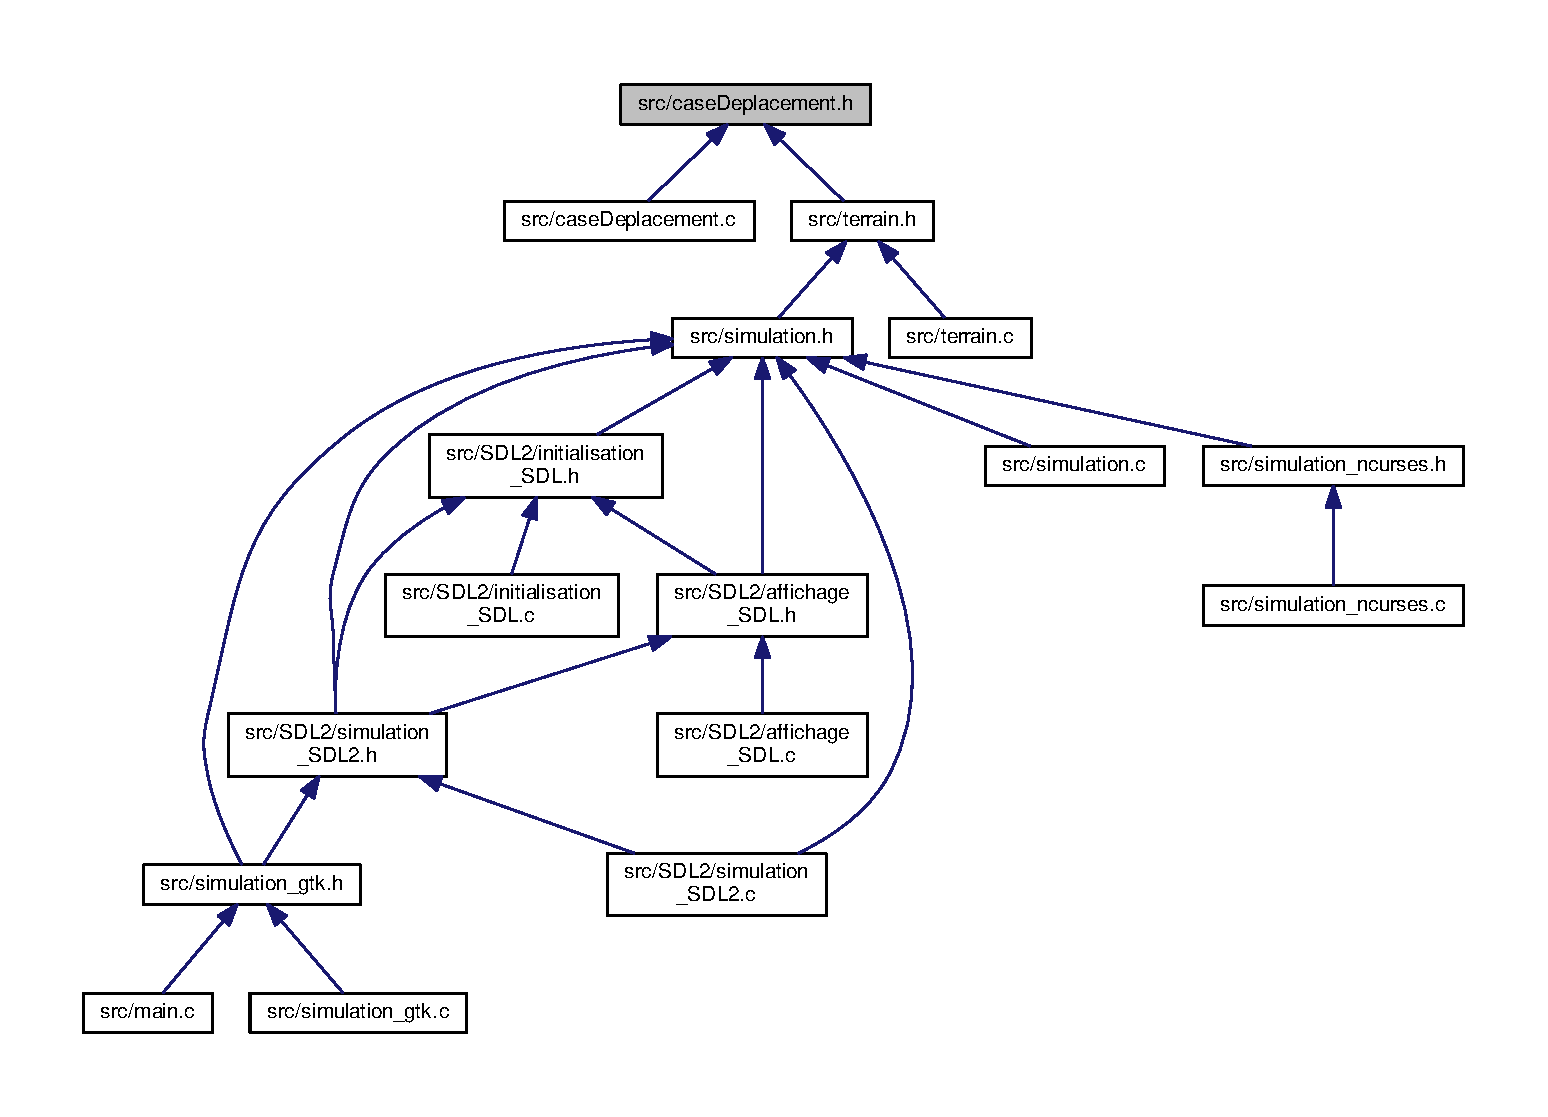
\includegraphics[width=350pt]{caseDeplacement_8h__dep__incl}
\end{center}
\end{figure}
\subsection*{Classes}
\begin{DoxyCompactItemize}
\item 
struct \hyperlink{structMCaseDeplacement}{M\+Case\+Deplacement}
\begin{DoxyCompactList}\small\item\em Structure definissant les cases de déplacement (champs d\textquotesingle{}influences et environement) \end{DoxyCompactList}\end{DoxyCompactItemize}
\subsection*{Définitions de type}
\begin{DoxyCompactItemize}
\item 
typedef enum \hyperlink{caseDeplacement_8h_af9a4f51a2aa1485342c48472a9124d83}{env} \hyperlink{caseDeplacement_8h_a107472c8543a9f7036d3afb3bfc7c97e}{env}
\item 
typedef struct \hyperlink{structMCaseDeplacement}{M\+Case\+Deplacement} \hyperlink{caseDeplacement_8h_aeab4f22b99f0db8b549dab4e46e3ead4}{case\+Deplacement}
\end{DoxyCompactItemize}
\subsection*{Énumérations}
\begin{DoxyCompactItemize}
\item 
enum \hyperlink{caseDeplacement_8h_af9a4f51a2aa1485342c48472a9124d83}{env} \{ \hyperlink{caseDeplacement_8h_af9a4f51a2aa1485342c48472a9124d83ad4686f4f969d0e851d9170c09a89a837}{V\+I\+DE}, 
\hyperlink{caseDeplacement_8h_af9a4f51a2aa1485342c48472a9124d83a4812eae6f742a8f18779779eeeffd570}{M\+UR}
 \}
\end{DoxyCompactItemize}
\subsection*{Fonctions}
\begin{DoxyCompactItemize}
\item 
enum \hyperlink{caseDeplacement_8h_af9a4f51a2aa1485342c48472a9124d83}{env} \hyperlink{caseDeplacement_8h_a3b6655cf83e6bc1c84ef1dd02f204e0b}{get\+Env\+Case} (\hyperlink{caseDeplacement_8h_aeab4f22b99f0db8b549dab4e46e3ead4}{case\+Deplacement} $\ast$p\+Case\+Dep)
\begin{DoxyCompactList}\small\item\em Recupère le type de case d\textquotesingle{}une case de deplacement. \end{DoxyCompactList}\item 
\hyperlink{personnage_8h_abd5c92a453bbf273f753b3f5b99da9e7}{Perso} $\ast$ \hyperlink{caseDeplacement_8h_a6b8c143eea4a9242b0f59a634c2f81b0}{get\+Perso\+Case} (\hyperlink{caseDeplacement_8h_aeab4f22b99f0db8b549dab4e46e3ead4}{case\+Deplacement} $\ast$p\+Case\+Dep)
\begin{DoxyCompactList}\small\item\em Recupère le personnage sur la case de déplacement. \end{DoxyCompactList}\item 
void \hyperlink{caseDeplacement_8h_ac9d21a1a61259ea3a3321fdec3661fea}{set\+Env\+Case} (\hyperlink{caseDeplacement_8h_aeab4f22b99f0db8b549dab4e46e3ead4}{case\+Deplacement} $\ast$p\+Case\+Dep, enum \hyperlink{caseDeplacement_8h_af9a4f51a2aa1485342c48472a9124d83}{env} valeur\+Env)
\begin{DoxyCompactList}\small\item\em Modifie le type de case d\textquotesingle{}une case de deplacement. \end{DoxyCompactList}\item 
void \hyperlink{caseDeplacement_8h_a2be2ab36936e9a5cb9fd2948353c7b12}{set\+Perso\+Case} (\hyperlink{caseDeplacement_8h_aeab4f22b99f0db8b549dab4e46e3ead4}{case\+Deplacement} $\ast$p\+Case\+Dep, \hyperlink{personnage_8h_abd5c92a453bbf273f753b3f5b99da9e7}{Perso} $\ast$p\+Perso)
\begin{DoxyCompactList}\small\item\em Modifie le personnage sur la case de déplacement. \end{DoxyCompactList}\item 
\hyperlink{caseDeplacement_8h_aeab4f22b99f0db8b549dab4e46e3ead4}{case\+Deplacement} $\ast$ \hyperlink{caseDeplacement_8h_a7ef31ff562e58ed644b58bc85dac2534}{init\+Case} (enum \hyperlink{caseDeplacement_8h_af9a4f51a2aa1485342c48472a9124d83}{env} env\+Case, \hyperlink{personnage_8h_abd5c92a453bbf273f753b3f5b99da9e7}{Perso} $\ast$p\+Perso)
\begin{DoxyCompactList}\small\item\em Crée et initialise une case de deplacement avec un type de case et un personnage dessus. \end{DoxyCompactList}\item 
unsigned short \hyperlink{caseDeplacement_8h_a271e610d4e5a86cabe14f2f9ae463442}{get\+Champ} (enum \hyperlink{personnage_8h_a3f6a2951aa3d5d428dd6d61e74db0d75}{type\+Perso} type, int id\+Perso, \hyperlink{caseDeplacement_8h_aeab4f22b99f0db8b549dab4e46e3ead4}{case\+Deplacement} $\ast$p\+Case\+Dep)
\begin{DoxyCompactList}\small\item\em Récupère la valeur du champ du perso défini par son type et son id sur une case. \end{DoxyCompactList}\item 
void \hyperlink{caseDeplacement_8h_a7b32586075b47b467bad6a2ab3bea8f6}{set\+Champ} (unsigned short intensite, enum \hyperlink{personnage_8h_a3f6a2951aa3d5d428dd6d61e74db0d75}{type\+Perso} type, int id\+Perso, \hyperlink{caseDeplacement_8h_aeab4f22b99f0db8b549dab4e46e3ead4}{case\+Deplacement} $\ast$p\+Case\+Dep)
\begin{DoxyCompactList}\small\item\em Définit la valeur du champ du perso défini par son type et son id sur une case. \end{DoxyCompactList}\end{DoxyCompactItemize}


\subsection{Description détaillée}
Définit une case sur lesquels les personnages vont pouvoir se déplacer. 



\subsection{Documentation des définitions de type}
\index{case\+Deplacement.\+h@{case\+Deplacement.\+h}!case\+Deplacement@{case\+Deplacement}}
\index{case\+Deplacement@{case\+Deplacement}!case\+Deplacement.\+h@{case\+Deplacement.\+h}}
\subsubsection[{\texorpdfstring{case\+Deplacement}{caseDeplacement}}]{\setlength{\rightskip}{0pt plus 5cm}typedef struct {\bf M\+Case\+Deplacement}  {\bf case\+Deplacement}}\hypertarget{caseDeplacement_8h_aeab4f22b99f0db8b549dab4e46e3ead4}{}\label{caseDeplacement_8h_aeab4f22b99f0db8b549dab4e46e3ead4}
\index{case\+Deplacement.\+h@{case\+Deplacement.\+h}!env@{env}}
\index{env@{env}!case\+Deplacement.\+h@{case\+Deplacement.\+h}}
\subsubsection[{\texorpdfstring{env}{env}}]{\setlength{\rightskip}{0pt plus 5cm}typedef enum {\bf env} {\bf env}}\hypertarget{caseDeplacement_8h_a107472c8543a9f7036d3afb3bfc7c97e}{}\label{caseDeplacement_8h_a107472c8543a9f7036d3afb3bfc7c97e}


\subsection{Documentation du type de l\textquotesingle{}énumération}
\index{case\+Deplacement.\+h@{case\+Deplacement.\+h}!env@{env}}
\index{env@{env}!case\+Deplacement.\+h@{case\+Deplacement.\+h}}
\subsubsection[{\texorpdfstring{env}{env}}]{\setlength{\rightskip}{0pt plus 5cm}enum {\bf env}}\hypertarget{caseDeplacement_8h_af9a4f51a2aa1485342c48472a9124d83}{}\label{caseDeplacement_8h_af9a4f51a2aa1485342c48472a9124d83}
env défini soit un mur soit le sol (vide) \begin{Desc}
\item[Valeurs énumérées]\par
\begin{description}
\index{V\+I\+DE@{V\+I\+DE}!case\+Deplacement.\+h@{case\+Deplacement.\+h}}\index{case\+Deplacement.\+h@{case\+Deplacement.\+h}!V\+I\+DE@{V\+I\+DE}}\item[{\em 
V\+I\+DE\hypertarget{caseDeplacement_8h_af9a4f51a2aa1485342c48472a9124d83ad4686f4f969d0e851d9170c09a89a837}{}\label{caseDeplacement_8h_af9a4f51a2aa1485342c48472a9124d83ad4686f4f969d0e851d9170c09a89a837}
}]\index{M\+UR@{M\+UR}!case\+Deplacement.\+h@{case\+Deplacement.\+h}}\index{case\+Deplacement.\+h@{case\+Deplacement.\+h}!M\+UR@{M\+UR}}\item[{\em 
M\+UR\hypertarget{caseDeplacement_8h_af9a4f51a2aa1485342c48472a9124d83a4812eae6f742a8f18779779eeeffd570}{}\label{caseDeplacement_8h_af9a4f51a2aa1485342c48472a9124d83a4812eae6f742a8f18779779eeeffd570}
}]\end{description}
\end{Desc}


\subsection{Documentation des fonctions}
\index{case\+Deplacement.\+h@{case\+Deplacement.\+h}!get\+Champ@{get\+Champ}}
\index{get\+Champ@{get\+Champ}!case\+Deplacement.\+h@{case\+Deplacement.\+h}}
\subsubsection[{\texorpdfstring{get\+Champ(enum type\+Perso type, int id\+Perso, case\+Deplacement $\ast$p\+Case\+Dep)}{getChamp(enum typePerso type, int idPerso, caseDeplacement *pCaseDep)}}]{\setlength{\rightskip}{0pt plus 5cm}unsigned short get\+Champ (
\begin{DoxyParamCaption}
\item[{enum {\bf type\+Perso}}]{type, }
\item[{int}]{id\+Perso, }
\item[{{\bf case\+Deplacement} $\ast$}]{p\+Case\+Dep}
\end{DoxyParamCaption}
)}\hypertarget{caseDeplacement_8h_a271e610d4e5a86cabe14f2f9ae463442}{}\label{caseDeplacement_8h_a271e610d4e5a86cabe14f2f9ae463442}


Récupère la valeur du champ du perso défini par son type et son id sur une case. 


\begin{DoxyParams}{Paramètres}
{\em type} & Type du perso (Z\+O\+M\+B\+IE, P\+O\+L\+I\+C\+I\+ER, C\+I\+T\+O\+Y\+EN) \\
\hline
{\em id\+Perso} & Id du perso dont on veut connaitre le champ \\
\hline
{\em p\+Case\+Dep} & Pointeur vers la case a detruire et liberer \\
\hline
\end{DoxyParams}
\index{case\+Deplacement.\+h@{case\+Deplacement.\+h}!get\+Env\+Case@{get\+Env\+Case}}
\index{get\+Env\+Case@{get\+Env\+Case}!case\+Deplacement.\+h@{case\+Deplacement.\+h}}
\subsubsection[{\texorpdfstring{get\+Env\+Case(case\+Deplacement $\ast$p\+Case\+Dep)}{getEnvCase(caseDeplacement *pCaseDep)}}]{\setlength{\rightskip}{0pt plus 5cm}enum {\bf env} get\+Env\+Case (
\begin{DoxyParamCaption}
\item[{{\bf case\+Deplacement} $\ast$}]{p\+Case\+Dep}
\end{DoxyParamCaption}
)}\hypertarget{caseDeplacement_8h_a3b6655cf83e6bc1c84ef1dd02f204e0b}{}\label{caseDeplacement_8h_a3b6655cf83e6bc1c84ef1dd02f204e0b}


Recupère le type de case d\textquotesingle{}une case de deplacement. 


\begin{DoxyParams}{Paramètres}
{\em p\+Case\+Dep} & Pointeur sur la case de déplacement à étudier \\
\hline
\end{DoxyParams}
\begin{DoxyReturn}{Renvoie}
Le type de case 
\end{DoxyReturn}
\index{case\+Deplacement.\+h@{case\+Deplacement.\+h}!get\+Perso\+Case@{get\+Perso\+Case}}
\index{get\+Perso\+Case@{get\+Perso\+Case}!case\+Deplacement.\+h@{case\+Deplacement.\+h}}
\subsubsection[{\texorpdfstring{get\+Perso\+Case(case\+Deplacement $\ast$p\+Case\+Dep)}{getPersoCase(caseDeplacement *pCaseDep)}}]{\setlength{\rightskip}{0pt plus 5cm}{\bf Perso}$\ast$ get\+Perso\+Case (
\begin{DoxyParamCaption}
\item[{{\bf case\+Deplacement} $\ast$}]{p\+Case\+Dep}
\end{DoxyParamCaption}
)}\hypertarget{caseDeplacement_8h_a6b8c143eea4a9242b0f59a634c2f81b0}{}\label{caseDeplacement_8h_a6b8c143eea4a9242b0f59a634c2f81b0}


Recupère le personnage sur la case de déplacement. 


\begin{DoxyParams}{Paramètres}
{\em p\+Case\+Dep} & Pointeur sur la case de déplacement à étudier \\
\hline
\end{DoxyParams}
\begin{DoxyReturn}{Renvoie}
Pointeur vers le personnage sur la case de déplacement 
\end{DoxyReturn}
\index{case\+Deplacement.\+h@{case\+Deplacement.\+h}!init\+Case@{init\+Case}}
\index{init\+Case@{init\+Case}!case\+Deplacement.\+h@{case\+Deplacement.\+h}}
\subsubsection[{\texorpdfstring{init\+Case(enum env env\+Case, Perso $\ast$p\+Perso)}{initCase(enum env envCase, Perso *pPerso)}}]{\setlength{\rightskip}{0pt plus 5cm}{\bf case\+Deplacement}$\ast$ init\+Case (
\begin{DoxyParamCaption}
\item[{enum {\bf env}}]{env\+Case, }
\item[{{\bf Perso} $\ast$}]{p\+Perso}
\end{DoxyParamCaption}
)}\hypertarget{caseDeplacement_8h_a7ef31ff562e58ed644b58bc85dac2534}{}\label{caseDeplacement_8h_a7ef31ff562e58ed644b58bc85dac2534}


Crée et initialise une case de deplacement avec un type de case et un personnage dessus. 


\begin{DoxyParams}{Paramètres}
{\em env\+Case} & Type de case \\
\hline
{\em p\+Perso} & Pointeur vers un personnage \\
\hline
\end{DoxyParams}
\begin{DoxyReturn}{Renvoie}
Pointeur vers cette case de deplacement 
\end{DoxyReturn}
\index{case\+Deplacement.\+h@{case\+Deplacement.\+h}!set\+Champ@{set\+Champ}}
\index{set\+Champ@{set\+Champ}!case\+Deplacement.\+h@{case\+Deplacement.\+h}}
\subsubsection[{\texorpdfstring{set\+Champ(unsigned short intensite, enum type\+Perso type, int id\+Perso, case\+Deplacement $\ast$p\+Case\+Dep)}{setChamp(unsigned short intensite, enum typePerso type, int idPerso, caseDeplacement *pCaseDep)}}]{\setlength{\rightskip}{0pt plus 5cm}void set\+Champ (
\begin{DoxyParamCaption}
\item[{unsigned short}]{intensite, }
\item[{enum {\bf type\+Perso}}]{type, }
\item[{int}]{id\+Perso, }
\item[{{\bf case\+Deplacement} $\ast$}]{p\+Case\+Dep}
\end{DoxyParamCaption}
)}\hypertarget{caseDeplacement_8h_a7b32586075b47b467bad6a2ab3bea8f6}{}\label{caseDeplacement_8h_a7b32586075b47b467bad6a2ab3bea8f6}


Définit la valeur du champ du perso défini par son type et son id sur une case. 


\begin{DoxyParams}{Paramètres}
{\em intensite} & La valeur du champs en p\+Case\+Dep \\
\hline
{\em type} & Type du perso (Z\+O\+M\+B\+IE, P\+O\+L\+I\+C\+I\+ER, C\+I\+T\+O\+Y\+EN) \\
\hline
{\em id\+Perso} & Id du perso dont on veut connaitre le champ \\
\hline
{\em p\+Case\+Dep} & Pointeur vers la case a detruire et liberer \\
\hline
\end{DoxyParams}
\index{case\+Deplacement.\+h@{case\+Deplacement.\+h}!set\+Env\+Case@{set\+Env\+Case}}
\index{set\+Env\+Case@{set\+Env\+Case}!case\+Deplacement.\+h@{case\+Deplacement.\+h}}
\subsubsection[{\texorpdfstring{set\+Env\+Case(case\+Deplacement $\ast$p\+Case\+Dep, enum env valeur\+Env)}{setEnvCase(caseDeplacement *pCaseDep, enum env valeurEnv)}}]{\setlength{\rightskip}{0pt plus 5cm}void set\+Env\+Case (
\begin{DoxyParamCaption}
\item[{{\bf case\+Deplacement} $\ast$}]{p\+Case\+Dep, }
\item[{enum {\bf env}}]{valeur\+Env}
\end{DoxyParamCaption}
)}\hypertarget{caseDeplacement_8h_ac9d21a1a61259ea3a3321fdec3661fea}{}\label{caseDeplacement_8h_ac9d21a1a61259ea3a3321fdec3661fea}


Modifie le type de case d\textquotesingle{}une case de deplacement. 


\begin{DoxyParams}{Paramètres}
{\em p\+Case\+Dep} & Pointeur sur la case de déplacement à étudier \\
\hline
{\em valeur\+Env} & Le type de case \\
\hline
\end{DoxyParams}
\index{case\+Deplacement.\+h@{case\+Deplacement.\+h}!set\+Perso\+Case@{set\+Perso\+Case}}
\index{set\+Perso\+Case@{set\+Perso\+Case}!case\+Deplacement.\+h@{case\+Deplacement.\+h}}
\subsubsection[{\texorpdfstring{set\+Perso\+Case(case\+Deplacement $\ast$p\+Case\+Dep, Perso $\ast$p\+Perso)}{setPersoCase(caseDeplacement *pCaseDep, Perso *pPerso)}}]{\setlength{\rightskip}{0pt plus 5cm}void set\+Perso\+Case (
\begin{DoxyParamCaption}
\item[{{\bf case\+Deplacement} $\ast$}]{p\+Case\+Dep, }
\item[{{\bf Perso} $\ast$}]{p\+Perso}
\end{DoxyParamCaption}
)}\hypertarget{caseDeplacement_8h_a2be2ab36936e9a5cb9fd2948353c7b12}{}\label{caseDeplacement_8h_a2be2ab36936e9a5cb9fd2948353c7b12}


Modifie le personnage sur la case de déplacement. 


\begin{DoxyParams}{Paramètres}
{\em p\+Case\+Dep} & Pointeur sur la case de déplacement à étudier \\
\hline
{\em p\+Perso} & Pointeur vers le personnage a mettre sur la case de déplacement \\
\hline
\end{DoxyParams}

\hypertarget{coordonnees_8c}{}\section{Référence du fichier src/coordonnees.c}
\label{coordonnees_8c}\index{src/coordonnees.\+c@{src/coordonnees.\+c}}
{\ttfamily \#include \char`\"{}coordonnees.\+h\char`\"{}}\\*
Graphe des dépendances par inclusion de coordonnees.\+c\+:
\nopagebreak
\begin{figure}[H]
\begin{center}
\leavevmode
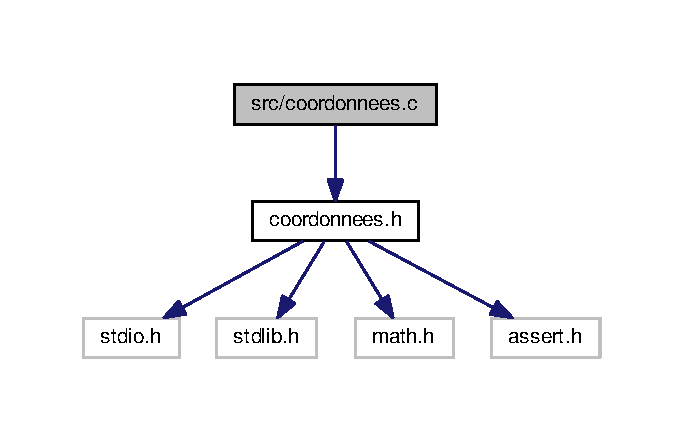
\includegraphics[width=328pt]{coordonnees_8c__incl}
\end{center}
\end{figure}
\subsection*{Fonctions}
\begin{DoxyCompactItemize}
\item 
void \hyperlink{coordonnees_8c_a8aff12a5cb5f0533906de5d33d6b70c7}{set\+X\+Coord\+\_\+\+Coord} (int x, \hyperlink{coordonnees_8h_a79929cdfee7bd985a5e4e25276bb3ba9}{Coordonnees} $\ast$p\+Coord)
\begin{DoxyCompactList}\small\item\em Edition de x\+Coord dans la structure. \end{DoxyCompactList}\item 
void \hyperlink{coordonnees_8c_ab348ef93b59b6b652cdeff4bcc65463e}{set\+Y\+Coord\+\_\+\+Coord} (int y, \hyperlink{coordonnees_8h_a79929cdfee7bd985a5e4e25276bb3ba9}{Coordonnees} $\ast$p\+Coord)
\begin{DoxyCompactList}\small\item\em Edition de y\+Coord dans la structure. \end{DoxyCompactList}\item 
void \hyperlink{coordonnees_8c_a0551295b10d2256fdc606611c3f7bb8b}{set\+X\+Y\+Coord\+\_\+\+Coord} (int x, int y, \hyperlink{coordonnees_8h_a79929cdfee7bd985a5e4e25276bb3ba9}{Coordonnees} $\ast$p\+Coord)
\begin{DoxyCompactList}\small\item\em Edition de x\+Coord et de y\+Coord dans la structure. \end{DoxyCompactList}\item 
int \hyperlink{coordonnees_8c_a48eda9077b4d340681e26693e29c8195}{get\+X\+Coord\+\_\+\+Coord} (\hyperlink{coordonnees_8h_a79929cdfee7bd985a5e4e25276bb3ba9}{Coordonnees} $\ast$p\+Coord)
\begin{DoxyCompactList}\small\item\em Recupère x\+Coord. \end{DoxyCompactList}\item 
int \hyperlink{coordonnees_8c_a40d9c810656479195c388fa1c776d6d8}{get\+Y\+Coord\+\_\+\+Coord} (\hyperlink{coordonnees_8h_a79929cdfee7bd985a5e4e25276bb3ba9}{Coordonnees} $\ast$p\+Coord)
\begin{DoxyCompactList}\small\item\em Recupère y\+Coord. \end{DoxyCompactList}\item 
\hyperlink{coordonnees_8h_a79929cdfee7bd985a5e4e25276bb3ba9}{Coordonnees} \hyperlink{coordonnees_8c_aafd58dbb37b1ce271a97809e08abd978}{get\+Coord\+Case\+Droite\+By\+X\+Y\+\_\+terr} (int x, int y)
\begin{DoxyCompactList}\small\item\em Retourne des coordonnées de la case à droite des coordonnées X/Y. \end{DoxyCompactList}\item 
\hyperlink{coordonnees_8h_a79929cdfee7bd985a5e4e25276bb3ba9}{Coordonnees} \hyperlink{coordonnees_8c_abd0e04f3069639088754f073df30b8d2}{get\+Coord\+Case\+Gauche\+By\+X\+Y\+\_\+terr} (int x, int y)
\begin{DoxyCompactList}\small\item\em Retourne des coordonnées de la case à gauche des coordonnées X/Y. \end{DoxyCompactList}\item 
\hyperlink{coordonnees_8h_a79929cdfee7bd985a5e4e25276bb3ba9}{Coordonnees} \hyperlink{coordonnees_8c_a1a7a40e1f4d1aa2e24701a0d3e9082b1}{get\+Coord\+Case\+Haut\+By\+X\+Y\+\_\+terr} (int x, int y)
\begin{DoxyCompactList}\small\item\em Retourne des coordonnées de la case en haut des coordonnées X/Y. \end{DoxyCompactList}\item 
\hyperlink{coordonnees_8h_a79929cdfee7bd985a5e4e25276bb3ba9}{Coordonnees} \hyperlink{coordonnees_8c_a2f71dd7bc9972e801034567e10be73f1}{get\+Coord\+Case\+Bas\+By\+X\+Y\+\_\+terr} (int x, int y)
\begin{DoxyCompactList}\small\item\em Retourne des coordonnées de la case en dessous des coordonnées X/Y. \end{DoxyCompactList}\item 
\hyperlink{coordonnees_8h_a79929cdfee7bd985a5e4e25276bb3ba9}{Coordonnees} \hyperlink{coordonnees_8c_a868ff8a6ca726b637ffffae9972ff652}{get\+Coord\+Case2\+Droite\+By\+X\+Y\+\_\+terr} (int x, int y)
\begin{DoxyCompactList}\small\item\em Retourne des coordonnées de la 2eme case à droite des coordonnées X/Y. \end{DoxyCompactList}\item 
\hyperlink{coordonnees_8h_a79929cdfee7bd985a5e4e25276bb3ba9}{Coordonnees} \hyperlink{coordonnees_8c_a05fcc3308194d2d8f15e8302837af04f}{get\+Coord\+Case2\+Gauche\+By\+X\+Y\+\_\+terr} (int x, int y)
\begin{DoxyCompactList}\small\item\em Retourne des coordonnées de la 2eme case à gauche des coordonnées X/Y. \end{DoxyCompactList}\item 
\hyperlink{coordonnees_8h_a79929cdfee7bd985a5e4e25276bb3ba9}{Coordonnees} \hyperlink{coordonnees_8c_a1a930c19d91bcda857a9d7fec9805891}{get\+Coord\+Case2\+Haut\+By\+X\+Y\+\_\+terr} (int x, int y)
\begin{DoxyCompactList}\small\item\em Retourne des coordonnées de la 2eme case en haut des coordonnées X/Y. \end{DoxyCompactList}\item 
\hyperlink{coordonnees_8h_a79929cdfee7bd985a5e4e25276bb3ba9}{Coordonnees} \hyperlink{coordonnees_8c_a9480eabef95071a9fdf16c931416b73e}{get\+Coord\+Case2\+Bas\+By\+X\+Y\+\_\+terr} (int x, int y)
\begin{DoxyCompactList}\small\item\em Retourne des coordonnées de la 2eme case en bas des coordonnées X/Y. \end{DoxyCompactList}\item 
\hyperlink{coordonnees_8h_a79929cdfee7bd985a5e4e25276bb3ba9}{Coordonnees} \hyperlink{coordonnees_8c_a296239d2fde59208ca18f88b380b0e2c}{get\+Coord\+Case\+H\+D\+By\+X\+Y\+\_\+terr} (int x, int y)
\begin{DoxyCompactList}\small\item\em Retourne des coordonnées de la case en haut à droite des coordonnées X/Y. \end{DoxyCompactList}\item 
\hyperlink{coordonnees_8h_a79929cdfee7bd985a5e4e25276bb3ba9}{Coordonnees} \hyperlink{coordonnees_8c_a7dc1f0e0d69c06e304d9d1f8cd97d886}{get\+Coord\+Case\+B\+D\+By\+X\+Y\+\_\+terr} (int x, int y)
\begin{DoxyCompactList}\small\item\em Retourne des coordonnées de la case en bas à droite des coordonnées X/Y. \end{DoxyCompactList}\item 
\hyperlink{coordonnees_8h_a79929cdfee7bd985a5e4e25276bb3ba9}{Coordonnees} \hyperlink{coordonnees_8c_a477d630118dec1f77d095ba3eb8b373a}{get\+Coord\+Case\+B\+G\+By\+X\+Y\+\_\+terr} (int x, int y)
\begin{DoxyCompactList}\small\item\em Retourne des coordonnées de la case en bas à gauche des coordonnées X/Y. \end{DoxyCompactList}\item 
\hyperlink{coordonnees_8h_a79929cdfee7bd985a5e4e25276bb3ba9}{Coordonnees} \hyperlink{coordonnees_8c_a7e5298523f25d3bdb07082149740b6dc}{get\+Coord\+Case\+H\+G\+By\+X\+Y\+\_\+terr} (int x, int y)
\begin{DoxyCompactList}\small\item\em Retourne des coordonnées de la case en haut à gauche des coordonnées X/Y. \end{DoxyCompactList}\item 
\hyperlink{coordonnees_8h_a79929cdfee7bd985a5e4e25276bb3ba9}{Coordonnees} \hyperlink{coordonnees_8c_a27025f633eac2d41fdeb9d57691ea249}{get\+Coord\+Case\+Bas\+By\+Coord\+\_\+terr} (\hyperlink{coordonnees_8h_a79929cdfee7bd985a5e4e25276bb3ba9}{Coordonnees} $\ast$p\+Coord)
\begin{DoxyCompactList}\small\item\em Retourne des coordonnées de la case en dessous d\textquotesingle{}une structure de coordonnée. \end{DoxyCompactList}\item 
\hyperlink{coordonnees_8h_a79929cdfee7bd985a5e4e25276bb3ba9}{Coordonnees} \hyperlink{coordonnees_8c_a6a86c1be1c447447b80acb0c560dcae6}{get\+Coord\+Case\+Haut\+By\+Coord\+\_\+terr} (\hyperlink{coordonnees_8h_a79929cdfee7bd985a5e4e25276bb3ba9}{Coordonnees} $\ast$p\+Coord)
\begin{DoxyCompactList}\small\item\em Retourne des coordonnées de la case en haut d\textquotesingle{}une structure de coordonnée. \end{DoxyCompactList}\item 
\hyperlink{coordonnees_8h_a79929cdfee7bd985a5e4e25276bb3ba9}{Coordonnees} \hyperlink{coordonnees_8c_abd2d0de1459a2cfc78fd6e5afbdc11a5}{get\+Coord\+Case\+Droite\+By\+Coord\+\_\+terr} (\hyperlink{coordonnees_8h_a79929cdfee7bd985a5e4e25276bb3ba9}{Coordonnees} $\ast$p\+Coord)
\begin{DoxyCompactList}\small\item\em Retourne des coordonnées de la case à droite d\textquotesingle{}une structure de coordonnée. \end{DoxyCompactList}\item 
\hyperlink{coordonnees_8h_a79929cdfee7bd985a5e4e25276bb3ba9}{Coordonnees} \hyperlink{coordonnees_8c_a28bf00e63c6736da38f1e2f2913ce11d}{get\+Coord\+Case\+Gauche\+By\+Coord\+\_\+terr} (\hyperlink{coordonnees_8h_a79929cdfee7bd985a5e4e25276bb3ba9}{Coordonnees} $\ast$p\+Coord)
\begin{DoxyCompactList}\small\item\em Retourne des coordonnées de la case à gauche d\textquotesingle{}une structure de coordonnée. \end{DoxyCompactList}\item 
\hyperlink{coordonnees_8h_a79929cdfee7bd985a5e4e25276bb3ba9}{Coordonnees} \hyperlink{coordonnees_8c_a611d41db2b5c28115b99ec0113635ffc}{get\+Coord\+Case2\+Bas\+By\+Coord\+\_\+terr} (\hyperlink{coordonnees_8h_a79929cdfee7bd985a5e4e25276bb3ba9}{Coordonnees} $\ast$p\+Coord)
\begin{DoxyCompactList}\small\item\em Retourne des coordonnées de la 2eme case en bas à partir de coordonnées. \end{DoxyCompactList}\item 
\hyperlink{coordonnees_8h_a79929cdfee7bd985a5e4e25276bb3ba9}{Coordonnees} \hyperlink{coordonnees_8c_a3fbd55920dc671d5802977574b552a3a}{get\+Coord\+Case2\+Haut\+By\+Coord\+\_\+terr} (\hyperlink{coordonnees_8h_a79929cdfee7bd985a5e4e25276bb3ba9}{Coordonnees} $\ast$p\+Coord)
\begin{DoxyCompactList}\small\item\em Retourne des coordonnées de la 2eme case en haut à partir de coordonnées. \end{DoxyCompactList}\item 
\hyperlink{coordonnees_8h_a79929cdfee7bd985a5e4e25276bb3ba9}{Coordonnees} \hyperlink{coordonnees_8c_a268d68b3b4bf0a9eca1d4cac2e38d4e7}{get\+Coord\+Case2\+Droite\+By\+Coord\+\_\+terr} (\hyperlink{coordonnees_8h_a79929cdfee7bd985a5e4e25276bb3ba9}{Coordonnees} $\ast$p\+Coord)
\begin{DoxyCompactList}\small\item\em Retourne des coordonnées de la 2eme case à droite à partir de coordonnées. \end{DoxyCompactList}\item 
\hyperlink{coordonnees_8h_a79929cdfee7bd985a5e4e25276bb3ba9}{Coordonnees} \hyperlink{coordonnees_8c_a280ca53928088ad711c959b8ee3c2a81}{get\+Coord\+Case2\+Gauche\+By\+Coord\+\_\+terr} (\hyperlink{coordonnees_8h_a79929cdfee7bd985a5e4e25276bb3ba9}{Coordonnees} $\ast$p\+Coord)
\begin{DoxyCompactList}\small\item\em Retourne des coordonnées de la 2eme case à gauche à partir de coordonnées. \end{DoxyCompactList}\item 
\hyperlink{coordonnees_8h_a79929cdfee7bd985a5e4e25276bb3ba9}{Coordonnees} \hyperlink{coordonnees_8c_a1a988653b61291da9700913a893cfe14}{get\+Coord\+Case\+H\+D\+By\+Coord\+\_\+terr} (\hyperlink{coordonnees_8h_a79929cdfee7bd985a5e4e25276bb3ba9}{Coordonnees} $\ast$p\+Coord)
\begin{DoxyCompactList}\small\item\em Retourne des coordonnées de la case en haut à droite à partir de coordonnées. \end{DoxyCompactList}\item 
\hyperlink{coordonnees_8h_a79929cdfee7bd985a5e4e25276bb3ba9}{Coordonnees} \hyperlink{coordonnees_8c_a2da45ab8ad8e1e543c600a5dd3a1b905}{get\+Coord\+Case\+B\+D\+By\+Coord\+\_\+terr} (\hyperlink{coordonnees_8h_a79929cdfee7bd985a5e4e25276bb3ba9}{Coordonnees} $\ast$p\+Coord)
\begin{DoxyCompactList}\small\item\em Retourne des coordonnées de la case en bas à droite à partir de coordonnées. \end{DoxyCompactList}\item 
\hyperlink{coordonnees_8h_a79929cdfee7bd985a5e4e25276bb3ba9}{Coordonnees} \hyperlink{coordonnees_8c_a624c21a2b978d50e6601bad8f298190b}{get\+Coord\+Case\+B\+G\+By\+Coord\+\_\+terr} (\hyperlink{coordonnees_8h_a79929cdfee7bd985a5e4e25276bb3ba9}{Coordonnees} $\ast$p\+Coord)
\begin{DoxyCompactList}\small\item\em Retourne des coordonnées de la case en bas à gauche à partir de coordonnées. \end{DoxyCompactList}\item 
\hyperlink{coordonnees_8h_a79929cdfee7bd985a5e4e25276bb3ba9}{Coordonnees} \hyperlink{coordonnees_8c_a096126ba60788fa3cb8c14c12c3777d1}{get\+Coord\+Case\+H\+G\+By\+Coord\+\_\+terr} (\hyperlink{coordonnees_8h_a79929cdfee7bd985a5e4e25276bb3ba9}{Coordonnees} $\ast$p\+Coord)
\begin{DoxyCompactList}\small\item\em Retourne des coordonnées de la case en haut à gauche à partir de coordonnées. \end{DoxyCompactList}\item 
\hyperlink{coordonnees_8h_a79929cdfee7bd985a5e4e25276bb3ba9}{Coordonnees} $\ast$ \hyperlink{coordonnees_8c_aefad4fcb9d51c146999a9b0ee90e6b62}{init\+Coordonnees\+\_\+coord} (int x, int y)
\begin{DoxyCompactList}\small\item\em Crée et initialise des coordonnées avec les valeur XY. \end{DoxyCompactList}\item 
void \hyperlink{coordonnees_8c_a23c06b4d17cdb6008e96945dfd2ab043}{testament\+Coord} (\hyperlink{coordonnees_8h_a79929cdfee7bd985a5e4e25276bb3ba9}{Coordonnees} $\ast$p\+Coord)
\begin{DoxyCompactList}\small\item\em Détruit et libère des coordonnées. \end{DoxyCompactList}\item 
float \hyperlink{coordonnees_8c_ad691c01633ef08dc8831d0544ce01d40}{distance\+Entre\+Deux\+Coordonnees\+\_\+\+Coord} (\hyperlink{coordonnees_8h_a79929cdfee7bd985a5e4e25276bb3ba9}{Coordonnees} $\ast$p\+Coord1, \hyperlink{coordonnees_8h_a79929cdfee7bd985a5e4e25276bb3ba9}{Coordonnees} $\ast$p\+Coord2)
\begin{DoxyCompactList}\small\item\em Retourne la distance entre deux Coordonnees. \end{DoxyCompactList}\item 
int \hyperlink{coordonnees_8c_a15ae1d9835553c9ff38e0ee0ff6db8f5}{sont\+Egale\+\_\+\+Coord} (\hyperlink{coordonnees_8h_a79929cdfee7bd985a5e4e25276bb3ba9}{Coordonnees} $\ast$p\+Coord1, \hyperlink{coordonnees_8h_a79929cdfee7bd985a5e4e25276bb3ba9}{Coordonnees} $\ast$p\+Coord2)
\begin{DoxyCompactList}\small\item\em Vérifie si deux Coordonnees donné sont identiques. \end{DoxyCompactList}\item 
void \hyperlink{coordonnees_8c_abe42b4ebb96328b33c08361965c79512}{test\+Fonctions\+\_\+\+Coord} ()
\begin{DoxyCompactList}\small\item\em Fontion de test des fonctions du module Coordonnees. \end{DoxyCompactList}\end{DoxyCompactItemize}


\subsection{Documentation des fonctions}
\index{coordonnees.\+c@{coordonnees.\+c}!distance\+Entre\+Deux\+Coordonnees\+\_\+\+Coord@{distance\+Entre\+Deux\+Coordonnees\+\_\+\+Coord}}
\index{distance\+Entre\+Deux\+Coordonnees\+\_\+\+Coord@{distance\+Entre\+Deux\+Coordonnees\+\_\+\+Coord}!coordonnees.\+c@{coordonnees.\+c}}
\subsubsection[{\texorpdfstring{distance\+Entre\+Deux\+Coordonnees\+\_\+\+Coord(\+Coordonnees $\ast$p\+Coord1, Coordonnees $\ast$p\+Coord2)}{distanceEntreDeuxCoordonnees_Coord(Coordonnees *pCoord1, Coordonnees *pCoord2)}}]{\setlength{\rightskip}{0pt plus 5cm}float distance\+Entre\+Deux\+Coordonnees\+\_\+\+Coord (
\begin{DoxyParamCaption}
\item[{{\bf Coordonnees} $\ast$}]{p\+Coord1, }
\item[{{\bf Coordonnees} $\ast$}]{p\+Coord2}
\end{DoxyParamCaption}
)}\hypertarget{coordonnees_8c_ad691c01633ef08dc8831d0544ce01d40}{}\label{coordonnees_8c_ad691c01633ef08dc8831d0544ce01d40}


Retourne la distance entre deux Coordonnees. 


\begin{DoxyParams}{Paramètres}
{\em coord1} & Coordonnees de la premier entitée \\
\hline
{\em coord2} & Coordonnees de la seconde entitée \\
\hline
\end{DoxyParams}
\begin{DoxyReturn}{Renvoie}
float représentant la distance entre ses deux coordonnées 
\end{DoxyReturn}
\index{coordonnees.\+c@{coordonnees.\+c}!get\+Coord\+Case2\+Bas\+By\+Coord\+\_\+terr@{get\+Coord\+Case2\+Bas\+By\+Coord\+\_\+terr}}
\index{get\+Coord\+Case2\+Bas\+By\+Coord\+\_\+terr@{get\+Coord\+Case2\+Bas\+By\+Coord\+\_\+terr}!coordonnees.\+c@{coordonnees.\+c}}
\subsubsection[{\texorpdfstring{get\+Coord\+Case2\+Bas\+By\+Coord\+\_\+terr(\+Coordonnees $\ast$p\+Coord)}{getCoordCase2BasByCoord_terr(Coordonnees *pCoord)}}]{\setlength{\rightskip}{0pt plus 5cm}{\bf Coordonnees} get\+Coord\+Case2\+Bas\+By\+Coord\+\_\+terr (
\begin{DoxyParamCaption}
\item[{{\bf Coordonnees} $\ast$}]{p\+Coord}
\end{DoxyParamCaption}
)}\hypertarget{coordonnees_8c_a611d41db2b5c28115b99ec0113635ffc}{}\label{coordonnees_8c_a611d41db2b5c28115b99ec0113635ffc}


Retourne des coordonnées de la 2eme case en bas à partir de coordonnées. 


\begin{DoxyParams}{Paramètres}
{\em coord} & Pointeur vers les coordonnées de référence \\
\hline
\end{DoxyParams}
\begin{DoxyReturn}{Renvoie}
Les coordonnées de la 2eme case en bas 
\end{DoxyReturn}
\index{coordonnees.\+c@{coordonnees.\+c}!get\+Coord\+Case2\+Bas\+By\+X\+Y\+\_\+terr@{get\+Coord\+Case2\+Bas\+By\+X\+Y\+\_\+terr}}
\index{get\+Coord\+Case2\+Bas\+By\+X\+Y\+\_\+terr@{get\+Coord\+Case2\+Bas\+By\+X\+Y\+\_\+terr}!coordonnees.\+c@{coordonnees.\+c}}
\subsubsection[{\texorpdfstring{get\+Coord\+Case2\+Bas\+By\+X\+Y\+\_\+terr(int x, int y)}{getCoordCase2BasByXY_terr(int x, int y)}}]{\setlength{\rightskip}{0pt plus 5cm}{\bf Coordonnees} get\+Coord\+Case2\+Bas\+By\+X\+Y\+\_\+terr (
\begin{DoxyParamCaption}
\item[{int}]{x, }
\item[{int}]{y}
\end{DoxyParamCaption}
)}\hypertarget{coordonnees_8c_a9480eabef95071a9fdf16c931416b73e}{}\label{coordonnees_8c_a9480eabef95071a9fdf16c931416b73e}


Retourne des coordonnées de la 2eme case en bas des coordonnées X/Y. 


\begin{DoxyParams}{Paramètres}
{\em x} & La coordonnées en X \\
\hline
{\em y} & La coordonnées en Y \\
\hline
\end{DoxyParams}
\begin{DoxyReturn}{Renvoie}
Les coordonnées de la 2eme case en bas 
\end{DoxyReturn}
\index{coordonnees.\+c@{coordonnees.\+c}!get\+Coord\+Case2\+Droite\+By\+Coord\+\_\+terr@{get\+Coord\+Case2\+Droite\+By\+Coord\+\_\+terr}}
\index{get\+Coord\+Case2\+Droite\+By\+Coord\+\_\+terr@{get\+Coord\+Case2\+Droite\+By\+Coord\+\_\+terr}!coordonnees.\+c@{coordonnees.\+c}}
\subsubsection[{\texorpdfstring{get\+Coord\+Case2\+Droite\+By\+Coord\+\_\+terr(\+Coordonnees $\ast$p\+Coord)}{getCoordCase2DroiteByCoord_terr(Coordonnees *pCoord)}}]{\setlength{\rightskip}{0pt plus 5cm}{\bf Coordonnees} get\+Coord\+Case2\+Droite\+By\+Coord\+\_\+terr (
\begin{DoxyParamCaption}
\item[{{\bf Coordonnees} $\ast$}]{p\+Coord}
\end{DoxyParamCaption}
)}\hypertarget{coordonnees_8c_a268d68b3b4bf0a9eca1d4cac2e38d4e7}{}\label{coordonnees_8c_a268d68b3b4bf0a9eca1d4cac2e38d4e7}


Retourne des coordonnées de la 2eme case à droite à partir de coordonnées. 


\begin{DoxyParams}{Paramètres}
{\em coord} & Pointeur vers les coordonnées de référence \\
\hline
\end{DoxyParams}
\begin{DoxyReturn}{Renvoie}
Les coordonnées de la 2eme case à droite 
\end{DoxyReturn}
\index{coordonnees.\+c@{coordonnees.\+c}!get\+Coord\+Case2\+Droite\+By\+X\+Y\+\_\+terr@{get\+Coord\+Case2\+Droite\+By\+X\+Y\+\_\+terr}}
\index{get\+Coord\+Case2\+Droite\+By\+X\+Y\+\_\+terr@{get\+Coord\+Case2\+Droite\+By\+X\+Y\+\_\+terr}!coordonnees.\+c@{coordonnees.\+c}}
\subsubsection[{\texorpdfstring{get\+Coord\+Case2\+Droite\+By\+X\+Y\+\_\+terr(int x, int y)}{getCoordCase2DroiteByXY_terr(int x, int y)}}]{\setlength{\rightskip}{0pt plus 5cm}{\bf Coordonnees} get\+Coord\+Case2\+Droite\+By\+X\+Y\+\_\+terr (
\begin{DoxyParamCaption}
\item[{int}]{x, }
\item[{int}]{y}
\end{DoxyParamCaption}
)}\hypertarget{coordonnees_8c_a868ff8a6ca726b637ffffae9972ff652}{}\label{coordonnees_8c_a868ff8a6ca726b637ffffae9972ff652}


Retourne des coordonnées de la 2eme case à droite des coordonnées X/Y. 


\begin{DoxyParams}{Paramètres}
{\em x} & La coordonnées en X \\
\hline
{\em y} & La coordonnées en Y \\
\hline
\end{DoxyParams}
\begin{DoxyReturn}{Renvoie}
Les coordonnées de la 2eme case à droite 
\end{DoxyReturn}
\index{coordonnees.\+c@{coordonnees.\+c}!get\+Coord\+Case2\+Gauche\+By\+Coord\+\_\+terr@{get\+Coord\+Case2\+Gauche\+By\+Coord\+\_\+terr}}
\index{get\+Coord\+Case2\+Gauche\+By\+Coord\+\_\+terr@{get\+Coord\+Case2\+Gauche\+By\+Coord\+\_\+terr}!coordonnees.\+c@{coordonnees.\+c}}
\subsubsection[{\texorpdfstring{get\+Coord\+Case2\+Gauche\+By\+Coord\+\_\+terr(\+Coordonnees $\ast$p\+Coord)}{getCoordCase2GaucheByCoord_terr(Coordonnees *pCoord)}}]{\setlength{\rightskip}{0pt plus 5cm}{\bf Coordonnees} get\+Coord\+Case2\+Gauche\+By\+Coord\+\_\+terr (
\begin{DoxyParamCaption}
\item[{{\bf Coordonnees} $\ast$}]{p\+Coord}
\end{DoxyParamCaption}
)}\hypertarget{coordonnees_8c_a280ca53928088ad711c959b8ee3c2a81}{}\label{coordonnees_8c_a280ca53928088ad711c959b8ee3c2a81}


Retourne des coordonnées de la 2eme case à gauche à partir de coordonnées. 


\begin{DoxyParams}{Paramètres}
{\em coord} & Pointeur vers les coordonnées de référence \\
\hline
\end{DoxyParams}
\begin{DoxyReturn}{Renvoie}
Les coordonnées de la 2eme case à gauche 
\end{DoxyReturn}
\index{coordonnees.\+c@{coordonnees.\+c}!get\+Coord\+Case2\+Gauche\+By\+X\+Y\+\_\+terr@{get\+Coord\+Case2\+Gauche\+By\+X\+Y\+\_\+terr}}
\index{get\+Coord\+Case2\+Gauche\+By\+X\+Y\+\_\+terr@{get\+Coord\+Case2\+Gauche\+By\+X\+Y\+\_\+terr}!coordonnees.\+c@{coordonnees.\+c}}
\subsubsection[{\texorpdfstring{get\+Coord\+Case2\+Gauche\+By\+X\+Y\+\_\+terr(int x, int y)}{getCoordCase2GaucheByXY_terr(int x, int y)}}]{\setlength{\rightskip}{0pt plus 5cm}{\bf Coordonnees} get\+Coord\+Case2\+Gauche\+By\+X\+Y\+\_\+terr (
\begin{DoxyParamCaption}
\item[{int}]{x, }
\item[{int}]{y}
\end{DoxyParamCaption}
)}\hypertarget{coordonnees_8c_a05fcc3308194d2d8f15e8302837af04f}{}\label{coordonnees_8c_a05fcc3308194d2d8f15e8302837af04f}


Retourne des coordonnées de la 2eme case à gauche des coordonnées X/Y. 


\begin{DoxyParams}{Paramètres}
{\em x} & La coordonnées en X \\
\hline
{\em y} & La coordonnées en Y \\
\hline
\end{DoxyParams}
\begin{DoxyReturn}{Renvoie}
Les coordonnées de la 2eme case à gauche 
\end{DoxyReturn}
\index{coordonnees.\+c@{coordonnees.\+c}!get\+Coord\+Case2\+Haut\+By\+Coord\+\_\+terr@{get\+Coord\+Case2\+Haut\+By\+Coord\+\_\+terr}}
\index{get\+Coord\+Case2\+Haut\+By\+Coord\+\_\+terr@{get\+Coord\+Case2\+Haut\+By\+Coord\+\_\+terr}!coordonnees.\+c@{coordonnees.\+c}}
\subsubsection[{\texorpdfstring{get\+Coord\+Case2\+Haut\+By\+Coord\+\_\+terr(\+Coordonnees $\ast$p\+Coord)}{getCoordCase2HautByCoord_terr(Coordonnees *pCoord)}}]{\setlength{\rightskip}{0pt plus 5cm}{\bf Coordonnees} get\+Coord\+Case2\+Haut\+By\+Coord\+\_\+terr (
\begin{DoxyParamCaption}
\item[{{\bf Coordonnees} $\ast$}]{p\+Coord}
\end{DoxyParamCaption}
)}\hypertarget{coordonnees_8c_a3fbd55920dc671d5802977574b552a3a}{}\label{coordonnees_8c_a3fbd55920dc671d5802977574b552a3a}


Retourne des coordonnées de la 2eme case en haut à partir de coordonnées. 


\begin{DoxyParams}{Paramètres}
{\em coord} & Pointeur vers les coordonnées de référence \\
\hline
\end{DoxyParams}
\begin{DoxyReturn}{Renvoie}
Les coordonnées de la 2eme case en haut 
\end{DoxyReturn}
\index{coordonnees.\+c@{coordonnees.\+c}!get\+Coord\+Case2\+Haut\+By\+X\+Y\+\_\+terr@{get\+Coord\+Case2\+Haut\+By\+X\+Y\+\_\+terr}}
\index{get\+Coord\+Case2\+Haut\+By\+X\+Y\+\_\+terr@{get\+Coord\+Case2\+Haut\+By\+X\+Y\+\_\+terr}!coordonnees.\+c@{coordonnees.\+c}}
\subsubsection[{\texorpdfstring{get\+Coord\+Case2\+Haut\+By\+X\+Y\+\_\+terr(int x, int y)}{getCoordCase2HautByXY_terr(int x, int y)}}]{\setlength{\rightskip}{0pt plus 5cm}{\bf Coordonnees} get\+Coord\+Case2\+Haut\+By\+X\+Y\+\_\+terr (
\begin{DoxyParamCaption}
\item[{int}]{x, }
\item[{int}]{y}
\end{DoxyParamCaption}
)}\hypertarget{coordonnees_8c_a1a930c19d91bcda857a9d7fec9805891}{}\label{coordonnees_8c_a1a930c19d91bcda857a9d7fec9805891}


Retourne des coordonnées de la 2eme case en haut des coordonnées X/Y. 


\begin{DoxyParams}{Paramètres}
{\em x} & La coordonnées en X \\
\hline
{\em y} & La coordonnées en Y \\
\hline
\end{DoxyParams}
\begin{DoxyReturn}{Renvoie}
Les coordonnées de la 2eme case en haut 
\end{DoxyReturn}
\index{coordonnees.\+c@{coordonnees.\+c}!get\+Coord\+Case\+Bas\+By\+Coord\+\_\+terr@{get\+Coord\+Case\+Bas\+By\+Coord\+\_\+terr}}
\index{get\+Coord\+Case\+Bas\+By\+Coord\+\_\+terr@{get\+Coord\+Case\+Bas\+By\+Coord\+\_\+terr}!coordonnees.\+c@{coordonnees.\+c}}
\subsubsection[{\texorpdfstring{get\+Coord\+Case\+Bas\+By\+Coord\+\_\+terr(\+Coordonnees $\ast$p\+Coord)}{getCoordCaseBasByCoord_terr(Coordonnees *pCoord)}}]{\setlength{\rightskip}{0pt plus 5cm}{\bf Coordonnees} get\+Coord\+Case\+Bas\+By\+Coord\+\_\+terr (
\begin{DoxyParamCaption}
\item[{{\bf Coordonnees} $\ast$}]{p\+Coord}
\end{DoxyParamCaption}
)}\hypertarget{coordonnees_8c_a27025f633eac2d41fdeb9d57691ea249}{}\label{coordonnees_8c_a27025f633eac2d41fdeb9d57691ea249}


Retourne des coordonnées de la case en dessous d\textquotesingle{}une structure de coordonnée. 


\begin{DoxyParams}{Paramètres}
{\em coord} & Pointeur sur les coordonnées de reference \\
\hline
\end{DoxyParams}
\begin{DoxyReturn}{Renvoie}
Les coordonnées de la case en dessous 
\end{DoxyReturn}
\index{coordonnees.\+c@{coordonnees.\+c}!get\+Coord\+Case\+Bas\+By\+X\+Y\+\_\+terr@{get\+Coord\+Case\+Bas\+By\+X\+Y\+\_\+terr}}
\index{get\+Coord\+Case\+Bas\+By\+X\+Y\+\_\+terr@{get\+Coord\+Case\+Bas\+By\+X\+Y\+\_\+terr}!coordonnees.\+c@{coordonnees.\+c}}
\subsubsection[{\texorpdfstring{get\+Coord\+Case\+Bas\+By\+X\+Y\+\_\+terr(int x, int y)}{getCoordCaseBasByXY_terr(int x, int y)}}]{\setlength{\rightskip}{0pt plus 5cm}{\bf Coordonnees} get\+Coord\+Case\+Bas\+By\+X\+Y\+\_\+terr (
\begin{DoxyParamCaption}
\item[{int}]{x, }
\item[{int}]{y}
\end{DoxyParamCaption}
)}\hypertarget{coordonnees_8c_a2f71dd7bc9972e801034567e10be73f1}{}\label{coordonnees_8c_a2f71dd7bc9972e801034567e10be73f1}


Retourne des coordonnées de la case en dessous des coordonnées X/Y. 


\begin{DoxyParams}{Paramètres}
{\em x} & La coordonnées en X \\
\hline
{\em y} & La coordonnées en Y \\
\hline
\end{DoxyParams}
\begin{DoxyReturn}{Renvoie}
Les coordonnées de la case en dessous 
\end{DoxyReturn}
\index{coordonnees.\+c@{coordonnees.\+c}!get\+Coord\+Case\+B\+D\+By\+Coord\+\_\+terr@{get\+Coord\+Case\+B\+D\+By\+Coord\+\_\+terr}}
\index{get\+Coord\+Case\+B\+D\+By\+Coord\+\_\+terr@{get\+Coord\+Case\+B\+D\+By\+Coord\+\_\+terr}!coordonnees.\+c@{coordonnees.\+c}}
\subsubsection[{\texorpdfstring{get\+Coord\+Case\+B\+D\+By\+Coord\+\_\+terr(\+Coordonnees $\ast$p\+Coord)}{getCoordCaseBDByCoord_terr(Coordonnees *pCoord)}}]{\setlength{\rightskip}{0pt plus 5cm}{\bf Coordonnees} get\+Coord\+Case\+B\+D\+By\+Coord\+\_\+terr (
\begin{DoxyParamCaption}
\item[{{\bf Coordonnees} $\ast$}]{p\+Coord}
\end{DoxyParamCaption}
)}\hypertarget{coordonnees_8c_a2da45ab8ad8e1e543c600a5dd3a1b905}{}\label{coordonnees_8c_a2da45ab8ad8e1e543c600a5dd3a1b905}


Retourne des coordonnées de la case en bas à droite à partir de coordonnées. 


\begin{DoxyParams}{Paramètres}
{\em coord} & Pointeur vers les coordonnées de référence \\
\hline
\end{DoxyParams}
\begin{DoxyReturn}{Renvoie}
Les coordonnées de la 2eme case en bas à droite 
\end{DoxyReturn}
\index{coordonnees.\+c@{coordonnees.\+c}!get\+Coord\+Case\+B\+D\+By\+X\+Y\+\_\+terr@{get\+Coord\+Case\+B\+D\+By\+X\+Y\+\_\+terr}}
\index{get\+Coord\+Case\+B\+D\+By\+X\+Y\+\_\+terr@{get\+Coord\+Case\+B\+D\+By\+X\+Y\+\_\+terr}!coordonnees.\+c@{coordonnees.\+c}}
\subsubsection[{\texorpdfstring{get\+Coord\+Case\+B\+D\+By\+X\+Y\+\_\+terr(int x, int y)}{getCoordCaseBDByXY_terr(int x, int y)}}]{\setlength{\rightskip}{0pt plus 5cm}{\bf Coordonnees} get\+Coord\+Case\+B\+D\+By\+X\+Y\+\_\+terr (
\begin{DoxyParamCaption}
\item[{int}]{x, }
\item[{int}]{y}
\end{DoxyParamCaption}
)}\hypertarget{coordonnees_8c_a7dc1f0e0d69c06e304d9d1f8cd97d886}{}\label{coordonnees_8c_a7dc1f0e0d69c06e304d9d1f8cd97d886}


Retourne des coordonnées de la case en bas à droite des coordonnées X/Y. 


\begin{DoxyParams}{Paramètres}
{\em x} & La coordonnées en X \\
\hline
{\em y} & La coordonnées en Y \\
\hline
\end{DoxyParams}
\begin{DoxyReturn}{Renvoie}
Les coordonnées de la case en bas à droite 
\end{DoxyReturn}
\index{coordonnees.\+c@{coordonnees.\+c}!get\+Coord\+Case\+B\+G\+By\+Coord\+\_\+terr@{get\+Coord\+Case\+B\+G\+By\+Coord\+\_\+terr}}
\index{get\+Coord\+Case\+B\+G\+By\+Coord\+\_\+terr@{get\+Coord\+Case\+B\+G\+By\+Coord\+\_\+terr}!coordonnees.\+c@{coordonnees.\+c}}
\subsubsection[{\texorpdfstring{get\+Coord\+Case\+B\+G\+By\+Coord\+\_\+terr(\+Coordonnees $\ast$p\+Coord)}{getCoordCaseBGByCoord_terr(Coordonnees *pCoord)}}]{\setlength{\rightskip}{0pt plus 5cm}{\bf Coordonnees} get\+Coord\+Case\+B\+G\+By\+Coord\+\_\+terr (
\begin{DoxyParamCaption}
\item[{{\bf Coordonnees} $\ast$}]{p\+Coord}
\end{DoxyParamCaption}
)}\hypertarget{coordonnees_8c_a624c21a2b978d50e6601bad8f298190b}{}\label{coordonnees_8c_a624c21a2b978d50e6601bad8f298190b}


Retourne des coordonnées de la case en bas à gauche à partir de coordonnées. 


\begin{DoxyParams}{Paramètres}
{\em coord} & Pointeur vers les coordonnées de référence \\
\hline
\end{DoxyParams}
\begin{DoxyReturn}{Renvoie}
Les coordonnées de la 2eme case en bas à gauche 
\end{DoxyReturn}
\index{coordonnees.\+c@{coordonnees.\+c}!get\+Coord\+Case\+B\+G\+By\+X\+Y\+\_\+terr@{get\+Coord\+Case\+B\+G\+By\+X\+Y\+\_\+terr}}
\index{get\+Coord\+Case\+B\+G\+By\+X\+Y\+\_\+terr@{get\+Coord\+Case\+B\+G\+By\+X\+Y\+\_\+terr}!coordonnees.\+c@{coordonnees.\+c}}
\subsubsection[{\texorpdfstring{get\+Coord\+Case\+B\+G\+By\+X\+Y\+\_\+terr(int x, int y)}{getCoordCaseBGByXY_terr(int x, int y)}}]{\setlength{\rightskip}{0pt plus 5cm}{\bf Coordonnees} get\+Coord\+Case\+B\+G\+By\+X\+Y\+\_\+terr (
\begin{DoxyParamCaption}
\item[{int}]{x, }
\item[{int}]{y}
\end{DoxyParamCaption}
)}\hypertarget{coordonnees_8c_a477d630118dec1f77d095ba3eb8b373a}{}\label{coordonnees_8c_a477d630118dec1f77d095ba3eb8b373a}


Retourne des coordonnées de la case en bas à gauche des coordonnées X/Y. 


\begin{DoxyParams}{Paramètres}
{\em x} & La coordonnées en X \\
\hline
{\em y} & La coordonnées en Y \\
\hline
\end{DoxyParams}
\begin{DoxyReturn}{Renvoie}
Les coordonnées de la case en bas à gauche 
\end{DoxyReturn}
\index{coordonnees.\+c@{coordonnees.\+c}!get\+Coord\+Case\+Droite\+By\+Coord\+\_\+terr@{get\+Coord\+Case\+Droite\+By\+Coord\+\_\+terr}}
\index{get\+Coord\+Case\+Droite\+By\+Coord\+\_\+terr@{get\+Coord\+Case\+Droite\+By\+Coord\+\_\+terr}!coordonnees.\+c@{coordonnees.\+c}}
\subsubsection[{\texorpdfstring{get\+Coord\+Case\+Droite\+By\+Coord\+\_\+terr(\+Coordonnees $\ast$p\+Coord)}{getCoordCaseDroiteByCoord_terr(Coordonnees *pCoord)}}]{\setlength{\rightskip}{0pt plus 5cm}{\bf Coordonnees} get\+Coord\+Case\+Droite\+By\+Coord\+\_\+terr (
\begin{DoxyParamCaption}
\item[{{\bf Coordonnees} $\ast$}]{p\+Coord}
\end{DoxyParamCaption}
)}\hypertarget{coordonnees_8c_abd2d0de1459a2cfc78fd6e5afbdc11a5}{}\label{coordonnees_8c_abd2d0de1459a2cfc78fd6e5afbdc11a5}


Retourne des coordonnées de la case à droite d\textquotesingle{}une structure de coordonnée. 


\begin{DoxyParams}{Paramètres}
{\em coord} & Pointeur sur les coordonnées de reference \\
\hline
\end{DoxyParams}
\begin{DoxyReturn}{Renvoie}
Les coordonnées de la case à droite 
\end{DoxyReturn}
\index{coordonnees.\+c@{coordonnees.\+c}!get\+Coord\+Case\+Droite\+By\+X\+Y\+\_\+terr@{get\+Coord\+Case\+Droite\+By\+X\+Y\+\_\+terr}}
\index{get\+Coord\+Case\+Droite\+By\+X\+Y\+\_\+terr@{get\+Coord\+Case\+Droite\+By\+X\+Y\+\_\+terr}!coordonnees.\+c@{coordonnees.\+c}}
\subsubsection[{\texorpdfstring{get\+Coord\+Case\+Droite\+By\+X\+Y\+\_\+terr(int x, int y)}{getCoordCaseDroiteByXY_terr(int x, int y)}}]{\setlength{\rightskip}{0pt plus 5cm}{\bf Coordonnees} get\+Coord\+Case\+Droite\+By\+X\+Y\+\_\+terr (
\begin{DoxyParamCaption}
\item[{int}]{x, }
\item[{int}]{y}
\end{DoxyParamCaption}
)}\hypertarget{coordonnees_8c_aafd58dbb37b1ce271a97809e08abd978}{}\label{coordonnees_8c_aafd58dbb37b1ce271a97809e08abd978}


Retourne des coordonnées de la case à droite des coordonnées X/Y. 


\begin{DoxyParams}{Paramètres}
{\em x} & La coordonnées en X \\
\hline
{\em y} & La coordonnées en Y \\
\hline
\end{DoxyParams}
\begin{DoxyReturn}{Renvoie}
Les coordonnées de la case à droite 
\end{DoxyReturn}
\index{coordonnees.\+c@{coordonnees.\+c}!get\+Coord\+Case\+Gauche\+By\+Coord\+\_\+terr@{get\+Coord\+Case\+Gauche\+By\+Coord\+\_\+terr}}
\index{get\+Coord\+Case\+Gauche\+By\+Coord\+\_\+terr@{get\+Coord\+Case\+Gauche\+By\+Coord\+\_\+terr}!coordonnees.\+c@{coordonnees.\+c}}
\subsubsection[{\texorpdfstring{get\+Coord\+Case\+Gauche\+By\+Coord\+\_\+terr(\+Coordonnees $\ast$p\+Coord)}{getCoordCaseGaucheByCoord_terr(Coordonnees *pCoord)}}]{\setlength{\rightskip}{0pt plus 5cm}{\bf Coordonnees} get\+Coord\+Case\+Gauche\+By\+Coord\+\_\+terr (
\begin{DoxyParamCaption}
\item[{{\bf Coordonnees} $\ast$}]{p\+Coord}
\end{DoxyParamCaption}
)}\hypertarget{coordonnees_8c_a28bf00e63c6736da38f1e2f2913ce11d}{}\label{coordonnees_8c_a28bf00e63c6736da38f1e2f2913ce11d}


Retourne des coordonnées de la case à gauche d\textquotesingle{}une structure de coordonnée. 


\begin{DoxyParams}{Paramètres}
{\em coord} & Pointeur sur les coordonnées de reference \\
\hline
\end{DoxyParams}
\begin{DoxyReturn}{Renvoie}
Les coordonnées de la case à gauche 
\end{DoxyReturn}
\index{coordonnees.\+c@{coordonnees.\+c}!get\+Coord\+Case\+Gauche\+By\+X\+Y\+\_\+terr@{get\+Coord\+Case\+Gauche\+By\+X\+Y\+\_\+terr}}
\index{get\+Coord\+Case\+Gauche\+By\+X\+Y\+\_\+terr@{get\+Coord\+Case\+Gauche\+By\+X\+Y\+\_\+terr}!coordonnees.\+c@{coordonnees.\+c}}
\subsubsection[{\texorpdfstring{get\+Coord\+Case\+Gauche\+By\+X\+Y\+\_\+terr(int x, int y)}{getCoordCaseGaucheByXY_terr(int x, int y)}}]{\setlength{\rightskip}{0pt plus 5cm}{\bf Coordonnees} get\+Coord\+Case\+Gauche\+By\+X\+Y\+\_\+terr (
\begin{DoxyParamCaption}
\item[{int}]{x, }
\item[{int}]{y}
\end{DoxyParamCaption}
)}\hypertarget{coordonnees_8c_abd0e04f3069639088754f073df30b8d2}{}\label{coordonnees_8c_abd0e04f3069639088754f073df30b8d2}


Retourne des coordonnées de la case à gauche des coordonnées X/Y. 


\begin{DoxyParams}{Paramètres}
{\em x} & La coordonnées en X \\
\hline
{\em y} & La coordonnées en Y \\
\hline
\end{DoxyParams}
\begin{DoxyReturn}{Renvoie}
Les coordonnées de la case à gauche 
\end{DoxyReturn}
\index{coordonnees.\+c@{coordonnees.\+c}!get\+Coord\+Case\+Haut\+By\+Coord\+\_\+terr@{get\+Coord\+Case\+Haut\+By\+Coord\+\_\+terr}}
\index{get\+Coord\+Case\+Haut\+By\+Coord\+\_\+terr@{get\+Coord\+Case\+Haut\+By\+Coord\+\_\+terr}!coordonnees.\+c@{coordonnees.\+c}}
\subsubsection[{\texorpdfstring{get\+Coord\+Case\+Haut\+By\+Coord\+\_\+terr(\+Coordonnees $\ast$p\+Coord)}{getCoordCaseHautByCoord_terr(Coordonnees *pCoord)}}]{\setlength{\rightskip}{0pt plus 5cm}{\bf Coordonnees} get\+Coord\+Case\+Haut\+By\+Coord\+\_\+terr (
\begin{DoxyParamCaption}
\item[{{\bf Coordonnees} $\ast$}]{p\+Coord}
\end{DoxyParamCaption}
)}\hypertarget{coordonnees_8c_a6a86c1be1c447447b80acb0c560dcae6}{}\label{coordonnees_8c_a6a86c1be1c447447b80acb0c560dcae6}


Retourne des coordonnées de la case en haut d\textquotesingle{}une structure de coordonnée. 


\begin{DoxyParams}{Paramètres}
{\em coord} & Pointeur sur les coordonnées de reference \\
\hline
\end{DoxyParams}
\begin{DoxyReturn}{Renvoie}
Les coordonnées de la case en haut 
\end{DoxyReturn}
\index{coordonnees.\+c@{coordonnees.\+c}!get\+Coord\+Case\+Haut\+By\+X\+Y\+\_\+terr@{get\+Coord\+Case\+Haut\+By\+X\+Y\+\_\+terr}}
\index{get\+Coord\+Case\+Haut\+By\+X\+Y\+\_\+terr@{get\+Coord\+Case\+Haut\+By\+X\+Y\+\_\+terr}!coordonnees.\+c@{coordonnees.\+c}}
\subsubsection[{\texorpdfstring{get\+Coord\+Case\+Haut\+By\+X\+Y\+\_\+terr(int x, int y)}{getCoordCaseHautByXY_terr(int x, int y)}}]{\setlength{\rightskip}{0pt plus 5cm}{\bf Coordonnees} get\+Coord\+Case\+Haut\+By\+X\+Y\+\_\+terr (
\begin{DoxyParamCaption}
\item[{int}]{x, }
\item[{int}]{y}
\end{DoxyParamCaption}
)}\hypertarget{coordonnees_8c_a1a7a40e1f4d1aa2e24701a0d3e9082b1}{}\label{coordonnees_8c_a1a7a40e1f4d1aa2e24701a0d3e9082b1}


Retourne des coordonnées de la case en haut des coordonnées X/Y. 


\begin{DoxyParams}{Paramètres}
{\em x} & La coordonnées en X \\
\hline
{\em y} & La coordonnées en Y \\
\hline
\end{DoxyParams}
\begin{DoxyReturn}{Renvoie}
Les coordonnées de la case en haut 
\end{DoxyReturn}
\index{coordonnees.\+c@{coordonnees.\+c}!get\+Coord\+Case\+H\+D\+By\+Coord\+\_\+terr@{get\+Coord\+Case\+H\+D\+By\+Coord\+\_\+terr}}
\index{get\+Coord\+Case\+H\+D\+By\+Coord\+\_\+terr@{get\+Coord\+Case\+H\+D\+By\+Coord\+\_\+terr}!coordonnees.\+c@{coordonnees.\+c}}
\subsubsection[{\texorpdfstring{get\+Coord\+Case\+H\+D\+By\+Coord\+\_\+terr(\+Coordonnees $\ast$p\+Coord)}{getCoordCaseHDByCoord_terr(Coordonnees *pCoord)}}]{\setlength{\rightskip}{0pt plus 5cm}{\bf Coordonnees} get\+Coord\+Case\+H\+D\+By\+Coord\+\_\+terr (
\begin{DoxyParamCaption}
\item[{{\bf Coordonnees} $\ast$}]{p\+Coord}
\end{DoxyParamCaption}
)}\hypertarget{coordonnees_8c_a1a988653b61291da9700913a893cfe14}{}\label{coordonnees_8c_a1a988653b61291da9700913a893cfe14}


Retourne des coordonnées de la case en haut à droite à partir de coordonnées. 


\begin{DoxyParams}{Paramètres}
{\em coord} & Pointeur vers les coordonnées de référence \\
\hline
\end{DoxyParams}
\begin{DoxyReturn}{Renvoie}
Les coordonnées de la 2eme case en haut à droite 
\end{DoxyReturn}
\index{coordonnees.\+c@{coordonnees.\+c}!get\+Coord\+Case\+H\+D\+By\+X\+Y\+\_\+terr@{get\+Coord\+Case\+H\+D\+By\+X\+Y\+\_\+terr}}
\index{get\+Coord\+Case\+H\+D\+By\+X\+Y\+\_\+terr@{get\+Coord\+Case\+H\+D\+By\+X\+Y\+\_\+terr}!coordonnees.\+c@{coordonnees.\+c}}
\subsubsection[{\texorpdfstring{get\+Coord\+Case\+H\+D\+By\+X\+Y\+\_\+terr(int x, int y)}{getCoordCaseHDByXY_terr(int x, int y)}}]{\setlength{\rightskip}{0pt plus 5cm}{\bf Coordonnees} get\+Coord\+Case\+H\+D\+By\+X\+Y\+\_\+terr (
\begin{DoxyParamCaption}
\item[{int}]{x, }
\item[{int}]{y}
\end{DoxyParamCaption}
)}\hypertarget{coordonnees_8c_a296239d2fde59208ca18f88b380b0e2c}{}\label{coordonnees_8c_a296239d2fde59208ca18f88b380b0e2c}


Retourne des coordonnées de la case en haut à droite des coordonnées X/Y. 


\begin{DoxyParams}{Paramètres}
{\em x} & La coordonnées en X \\
\hline
{\em y} & La coordonnées en Y \\
\hline
\end{DoxyParams}
\begin{DoxyReturn}{Renvoie}
Les coordonnées de la case en haut à droite 
\end{DoxyReturn}
\index{coordonnees.\+c@{coordonnees.\+c}!get\+Coord\+Case\+H\+G\+By\+Coord\+\_\+terr@{get\+Coord\+Case\+H\+G\+By\+Coord\+\_\+terr}}
\index{get\+Coord\+Case\+H\+G\+By\+Coord\+\_\+terr@{get\+Coord\+Case\+H\+G\+By\+Coord\+\_\+terr}!coordonnees.\+c@{coordonnees.\+c}}
\subsubsection[{\texorpdfstring{get\+Coord\+Case\+H\+G\+By\+Coord\+\_\+terr(\+Coordonnees $\ast$p\+Coord)}{getCoordCaseHGByCoord_terr(Coordonnees *pCoord)}}]{\setlength{\rightskip}{0pt plus 5cm}{\bf Coordonnees} get\+Coord\+Case\+H\+G\+By\+Coord\+\_\+terr (
\begin{DoxyParamCaption}
\item[{{\bf Coordonnees} $\ast$}]{p\+Coord}
\end{DoxyParamCaption}
)}\hypertarget{coordonnees_8c_a096126ba60788fa3cb8c14c12c3777d1}{}\label{coordonnees_8c_a096126ba60788fa3cb8c14c12c3777d1}


Retourne des coordonnées de la case en haut à gauche à partir de coordonnées. 


\begin{DoxyParams}{Paramètres}
{\em coord} & Pointeur vers les coordonnées de référence \\
\hline
\end{DoxyParams}
\begin{DoxyReturn}{Renvoie}
Les coordonnées de la 2eme case en haut à gauche 
\end{DoxyReturn}
\index{coordonnees.\+c@{coordonnees.\+c}!get\+Coord\+Case\+H\+G\+By\+X\+Y\+\_\+terr@{get\+Coord\+Case\+H\+G\+By\+X\+Y\+\_\+terr}}
\index{get\+Coord\+Case\+H\+G\+By\+X\+Y\+\_\+terr@{get\+Coord\+Case\+H\+G\+By\+X\+Y\+\_\+terr}!coordonnees.\+c@{coordonnees.\+c}}
\subsubsection[{\texorpdfstring{get\+Coord\+Case\+H\+G\+By\+X\+Y\+\_\+terr(int x, int y)}{getCoordCaseHGByXY_terr(int x, int y)}}]{\setlength{\rightskip}{0pt plus 5cm}{\bf Coordonnees} get\+Coord\+Case\+H\+G\+By\+X\+Y\+\_\+terr (
\begin{DoxyParamCaption}
\item[{int}]{x, }
\item[{int}]{y}
\end{DoxyParamCaption}
)}\hypertarget{coordonnees_8c_a7e5298523f25d3bdb07082149740b6dc}{}\label{coordonnees_8c_a7e5298523f25d3bdb07082149740b6dc}


Retourne des coordonnées de la case en haut à gauche des coordonnées X/Y. 


\begin{DoxyParams}{Paramètres}
{\em x} & La coordonnées en X \\
\hline
{\em y} & La coordonnées en Y \\
\hline
\end{DoxyParams}
\begin{DoxyReturn}{Renvoie}
Les coordonnées de la case en haut à gauche 
\end{DoxyReturn}
\index{coordonnees.\+c@{coordonnees.\+c}!get\+X\+Coord\+\_\+\+Coord@{get\+X\+Coord\+\_\+\+Coord}}
\index{get\+X\+Coord\+\_\+\+Coord@{get\+X\+Coord\+\_\+\+Coord}!coordonnees.\+c@{coordonnees.\+c}}
\subsubsection[{\texorpdfstring{get\+X\+Coord\+\_\+\+Coord(\+Coordonnees $\ast$p\+Coord)}{getXCoord_Coord(Coordonnees *pCoord)}}]{\setlength{\rightskip}{0pt plus 5cm}int get\+X\+Coord\+\_\+\+Coord (
\begin{DoxyParamCaption}
\item[{{\bf Coordonnees} $\ast$}]{p\+Coord}
\end{DoxyParamCaption}
)}\hypertarget{coordonnees_8c_a48eda9077b4d340681e26693e29c8195}{}\label{coordonnees_8c_a48eda9077b4d340681e26693e29c8195}


Recupère x\+Coord. 


\begin{DoxyParams}{Paramètres}
{\em p\+Coord} & Pointeur sur la structure Coordonnees à lire \\
\hline
\end{DoxyParams}
\begin{DoxyReturn}{Renvoie}
La valeur de x\+Coord 
\end{DoxyReturn}
\index{coordonnees.\+c@{coordonnees.\+c}!get\+Y\+Coord\+\_\+\+Coord@{get\+Y\+Coord\+\_\+\+Coord}}
\index{get\+Y\+Coord\+\_\+\+Coord@{get\+Y\+Coord\+\_\+\+Coord}!coordonnees.\+c@{coordonnees.\+c}}
\subsubsection[{\texorpdfstring{get\+Y\+Coord\+\_\+\+Coord(\+Coordonnees $\ast$p\+Coord)}{getYCoord_Coord(Coordonnees *pCoord)}}]{\setlength{\rightskip}{0pt plus 5cm}int get\+Y\+Coord\+\_\+\+Coord (
\begin{DoxyParamCaption}
\item[{{\bf Coordonnees} $\ast$}]{p\+Coord}
\end{DoxyParamCaption}
)}\hypertarget{coordonnees_8c_a40d9c810656479195c388fa1c776d6d8}{}\label{coordonnees_8c_a40d9c810656479195c388fa1c776d6d8}


Recupère y\+Coord. 


\begin{DoxyParams}{Paramètres}
{\em p\+Coord} & Pointeur sur la structure Coordonnees à lire \\
\hline
\end{DoxyParams}
\begin{DoxyReturn}{Renvoie}
La valeur de Y\+Coord 
\end{DoxyReturn}
\index{coordonnees.\+c@{coordonnees.\+c}!init\+Coordonnees\+\_\+coord@{init\+Coordonnees\+\_\+coord}}
\index{init\+Coordonnees\+\_\+coord@{init\+Coordonnees\+\_\+coord}!coordonnees.\+c@{coordonnees.\+c}}
\subsubsection[{\texorpdfstring{init\+Coordonnees\+\_\+coord(int x, int y)}{initCoordonnees_coord(int x, int y)}}]{\setlength{\rightskip}{0pt plus 5cm}{\bf Coordonnees}$\ast$ init\+Coordonnees\+\_\+coord (
\begin{DoxyParamCaption}
\item[{int}]{x, }
\item[{int}]{y}
\end{DoxyParamCaption}
)}\hypertarget{coordonnees_8c_aefad4fcb9d51c146999a9b0ee90e6b62}{}\label{coordonnees_8c_aefad4fcb9d51c146999a9b0ee90e6b62}


Crée et initialise des coordonnées avec les valeur XY. 


\begin{DoxyParams}{Paramètres}
{\em x} & Entier de valeur de X \\
\hline
{\em y} & Entier de valeur de Y \\
\hline
\end{DoxyParams}
\begin{DoxyReturn}{Renvoie}
Des coordonnées initialisées 
\end{DoxyReturn}
\index{coordonnees.\+c@{coordonnees.\+c}!set\+X\+Coord\+\_\+\+Coord@{set\+X\+Coord\+\_\+\+Coord}}
\index{set\+X\+Coord\+\_\+\+Coord@{set\+X\+Coord\+\_\+\+Coord}!coordonnees.\+c@{coordonnees.\+c}}
\subsubsection[{\texorpdfstring{set\+X\+Coord\+\_\+\+Coord(int x, Coordonnees $\ast$p\+Coord)}{setXCoord_Coord(int x, Coordonnees *pCoord)}}]{\setlength{\rightskip}{0pt plus 5cm}void set\+X\+Coord\+\_\+\+Coord (
\begin{DoxyParamCaption}
\item[{int}]{x, }
\item[{{\bf Coordonnees} $\ast$}]{p\+Coord}
\end{DoxyParamCaption}
)}\hypertarget{coordonnees_8c_a8aff12a5cb5f0533906de5d33d6b70c7}{}\label{coordonnees_8c_a8aff12a5cb5f0533906de5d33d6b70c7}


Edition de x\+Coord dans la structure. 


\begin{DoxyParams}{Paramètres}
{\em x} & Valeur sur l\textquotesingle{}axe des x \\
\hline
{\em p\+Coord} & Pointeur sur la structure Coordonnees à editer \\
\hline
\end{DoxyParams}
\index{coordonnees.\+c@{coordonnees.\+c}!set\+X\+Y\+Coord\+\_\+\+Coord@{set\+X\+Y\+Coord\+\_\+\+Coord}}
\index{set\+X\+Y\+Coord\+\_\+\+Coord@{set\+X\+Y\+Coord\+\_\+\+Coord}!coordonnees.\+c@{coordonnees.\+c}}
\subsubsection[{\texorpdfstring{set\+X\+Y\+Coord\+\_\+\+Coord(int x, int y, Coordonnees $\ast$p\+Coord)}{setXYCoord_Coord(int x, int y, Coordonnees *pCoord)}}]{\setlength{\rightskip}{0pt plus 5cm}void set\+X\+Y\+Coord\+\_\+\+Coord (
\begin{DoxyParamCaption}
\item[{int}]{x, }
\item[{int}]{y, }
\item[{{\bf Coordonnees} $\ast$}]{p\+Coord}
\end{DoxyParamCaption}
)}\hypertarget{coordonnees_8c_a0551295b10d2256fdc606611c3f7bb8b}{}\label{coordonnees_8c_a0551295b10d2256fdc606611c3f7bb8b}


Edition de x\+Coord et de y\+Coord dans la structure. 


\begin{DoxyParams}{Paramètres}
{\em x\+Coord} & Valeur sur l\textquotesingle{}axe des x \\
\hline
{\em y\+Coord} & Valeur sur l\textquotesingle{}axe des y \\
\hline
{\em p\+Coord} & Pointeur sur la structure Coordonnees à editer \\
\hline
\end{DoxyParams}
\index{coordonnees.\+c@{coordonnees.\+c}!set\+Y\+Coord\+\_\+\+Coord@{set\+Y\+Coord\+\_\+\+Coord}}
\index{set\+Y\+Coord\+\_\+\+Coord@{set\+Y\+Coord\+\_\+\+Coord}!coordonnees.\+c@{coordonnees.\+c}}
\subsubsection[{\texorpdfstring{set\+Y\+Coord\+\_\+\+Coord(int y, Coordonnees $\ast$p\+Coord)}{setYCoord_Coord(int y, Coordonnees *pCoord)}}]{\setlength{\rightskip}{0pt plus 5cm}void set\+Y\+Coord\+\_\+\+Coord (
\begin{DoxyParamCaption}
\item[{int}]{y, }
\item[{{\bf Coordonnees} $\ast$}]{p\+Coord}
\end{DoxyParamCaption}
)}\hypertarget{coordonnees_8c_ab348ef93b59b6b652cdeff4bcc65463e}{}\label{coordonnees_8c_ab348ef93b59b6b652cdeff4bcc65463e}


Edition de y\+Coord dans la structure. 


\begin{DoxyParams}{Paramètres}
{\em y} & Valeur sur l\textquotesingle{}axe des y \\
\hline
{\em p\+Coord} & Pointeur sur la structure Coordonnees à editer \\
\hline
\end{DoxyParams}
\index{coordonnees.\+c@{coordonnees.\+c}!sont\+Egale\+\_\+\+Coord@{sont\+Egale\+\_\+\+Coord}}
\index{sont\+Egale\+\_\+\+Coord@{sont\+Egale\+\_\+\+Coord}!coordonnees.\+c@{coordonnees.\+c}}
\subsubsection[{\texorpdfstring{sont\+Egale\+\_\+\+Coord(\+Coordonnees $\ast$p\+Coord1, Coordonnees $\ast$p\+Coord2)}{sontEgale_Coord(Coordonnees *pCoord1, Coordonnees *pCoord2)}}]{\setlength{\rightskip}{0pt plus 5cm}int sont\+Egale\+\_\+\+Coord (
\begin{DoxyParamCaption}
\item[{{\bf Coordonnees} $\ast$}]{p\+Coord1, }
\item[{{\bf Coordonnees} $\ast$}]{p\+Coord2}
\end{DoxyParamCaption}
)}\hypertarget{coordonnees_8c_a15ae1d9835553c9ff38e0ee0ff6db8f5}{}\label{coordonnees_8c_a15ae1d9835553c9ff38e0ee0ff6db8f5}


Vérifie si deux Coordonnees donné sont identiques. 


\begin{DoxyParams}{Paramètres}
{\em coord1} & Coordonnees de la premier entitée \\
\hline
{\em coord2} & Coordonnees de la seconde entitée \\
\hline
\end{DoxyParams}
\begin{DoxyReturn}{Renvoie}
Retourne 1 si elles sont identique, 0 sinon 
\end{DoxyReturn}
\index{coordonnees.\+c@{coordonnees.\+c}!testament\+Coord@{testament\+Coord}}
\index{testament\+Coord@{testament\+Coord}!coordonnees.\+c@{coordonnees.\+c}}
\subsubsection[{\texorpdfstring{testament\+Coord(\+Coordonnees $\ast$p\+Coord)}{testamentCoord(Coordonnees *pCoord)}}]{\setlength{\rightskip}{0pt plus 5cm}void testament\+Coord (
\begin{DoxyParamCaption}
\item[{{\bf Coordonnees} $\ast$}]{p\+Coord}
\end{DoxyParamCaption}
)}\hypertarget{coordonnees_8c_a23c06b4d17cdb6008e96945dfd2ab043}{}\label{coordonnees_8c_a23c06b4d17cdb6008e96945dfd2ab043}


Détruit et libère des coordonnées. 


\begin{DoxyParams}{Paramètres}
{\em coord} & Les coordonnées a liberer et détruire \\
\hline
\end{DoxyParams}
\index{coordonnees.\+c@{coordonnees.\+c}!test\+Fonctions\+\_\+\+Coord@{test\+Fonctions\+\_\+\+Coord}}
\index{test\+Fonctions\+\_\+\+Coord@{test\+Fonctions\+\_\+\+Coord}!coordonnees.\+c@{coordonnees.\+c}}
\subsubsection[{\texorpdfstring{test\+Fonctions\+\_\+\+Coord()}{testFonctions_Coord()}}]{\setlength{\rightskip}{0pt plus 5cm}void test\+Fonctions\+\_\+\+Coord (
\begin{DoxyParamCaption}
{}
\end{DoxyParamCaption}
)}\hypertarget{coordonnees_8c_abe42b4ebb96328b33c08361965c79512}{}\label{coordonnees_8c_abe42b4ebb96328b33c08361965c79512}


Fontion de test des fonctions du module Coordonnees. 


\hypertarget{coordonnees_8h}{}\section{Référence du fichier src/coordonnees.h}
\label{coordonnees_8h}\index{src/coordonnees.\+h@{src/coordonnees.\+h}}


Définit les coordonnées atomiques du terrain et ses accesseurs.  


{\ttfamily \#include $<$stdio.\+h$>$}\\*
{\ttfamily \#include $<$stdlib.\+h$>$}\\*
{\ttfamily \#include $<$math.\+h$>$}\\*
{\ttfamily \#include $<$assert.\+h$>$}\\*
Graphe des dépendances par inclusion de coordonnees.\+h\+:\nopagebreak
\begin{figure}[H]
\begin{center}
\leavevmode
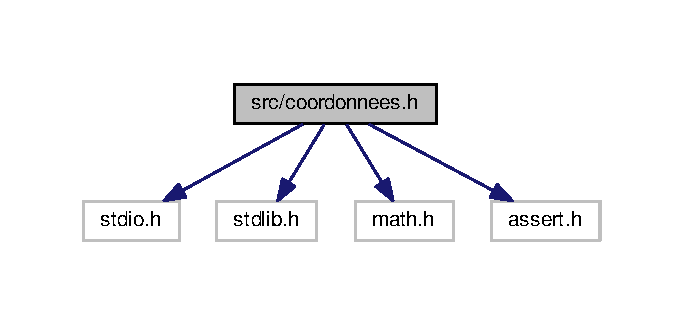
\includegraphics[width=328pt]{coordonnees_8h__incl}
\end{center}
\end{figure}
Ce graphe montre quels fichiers incluent directement ou indirectement ce fichier \+:\nopagebreak
\begin{figure}[H]
\begin{center}
\leavevmode
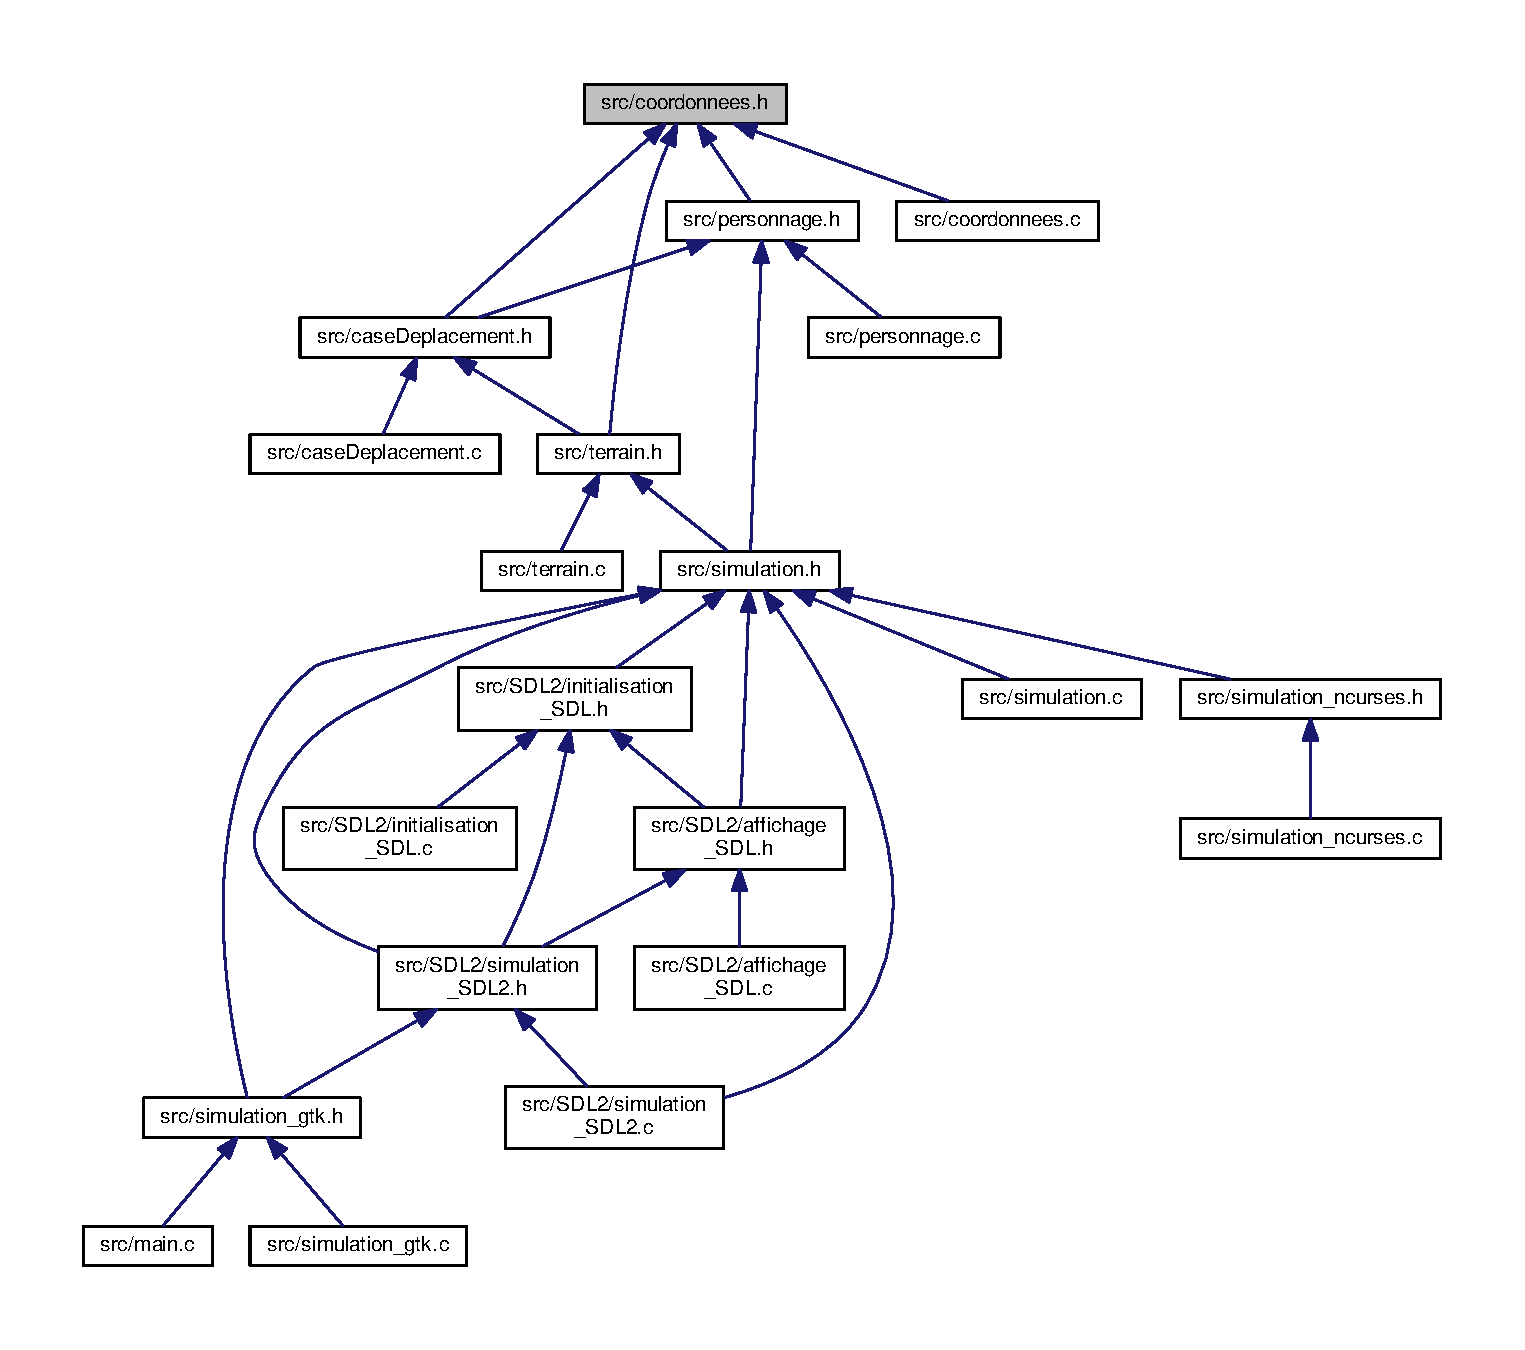
\includegraphics[width=350pt]{coordonnees_8h__dep__incl}
\end{center}
\end{figure}
\subsection*{Classes}
\begin{DoxyCompactItemize}
\item 
struct \hyperlink{structMCoordonnees}{M\+Coordonnees}
\begin{DoxyCompactList}\small\item\em Structure definissant des coordonnees en deux dimension (pour des entitées) \end{DoxyCompactList}\end{DoxyCompactItemize}
\subsection*{Définitions de type}
\begin{DoxyCompactItemize}
\item 
typedef struct \hyperlink{structMCoordonnees}{M\+Coordonnees} \hyperlink{coordonnees_8h_a79929cdfee7bd985a5e4e25276bb3ba9}{Coordonnees}
\end{DoxyCompactItemize}
\subsection*{Fonctions}
\begin{DoxyCompactItemize}
\item 
void \hyperlink{coordonnees_8h_a8aff12a5cb5f0533906de5d33d6b70c7}{set\+X\+Coord\+\_\+\+Coord} (int x, \hyperlink{coordonnees_8h_a79929cdfee7bd985a5e4e25276bb3ba9}{Coordonnees} $\ast$p\+Coord)
\begin{DoxyCompactList}\small\item\em Edition de x\+Coord dans la structure. \end{DoxyCompactList}\item 
void \hyperlink{coordonnees_8h_ab348ef93b59b6b652cdeff4bcc65463e}{set\+Y\+Coord\+\_\+\+Coord} (int y, \hyperlink{coordonnees_8h_a79929cdfee7bd985a5e4e25276bb3ba9}{Coordonnees} $\ast$p\+Coord)
\begin{DoxyCompactList}\small\item\em Edition de y\+Coord dans la structure. \end{DoxyCompactList}\item 
void \hyperlink{coordonnees_8h_a0551295b10d2256fdc606611c3f7bb8b}{set\+X\+Y\+Coord\+\_\+\+Coord} (int x, int y, \hyperlink{coordonnees_8h_a79929cdfee7bd985a5e4e25276bb3ba9}{Coordonnees} $\ast$p\+Coord)
\begin{DoxyCompactList}\small\item\em Edition de x\+Coord et de y\+Coord dans la structure. \end{DoxyCompactList}\item 
int \hyperlink{coordonnees_8h_a48eda9077b4d340681e26693e29c8195}{get\+X\+Coord\+\_\+\+Coord} (\hyperlink{coordonnees_8h_a79929cdfee7bd985a5e4e25276bb3ba9}{Coordonnees} $\ast$p\+Coord)
\begin{DoxyCompactList}\small\item\em Recupère x\+Coord. \end{DoxyCompactList}\item 
int \hyperlink{coordonnees_8h_a40d9c810656479195c388fa1c776d6d8}{get\+Y\+Coord\+\_\+\+Coord} (\hyperlink{coordonnees_8h_a79929cdfee7bd985a5e4e25276bb3ba9}{Coordonnees} $\ast$p\+Coord)
\begin{DoxyCompactList}\small\item\em Recupère y\+Coord. \end{DoxyCompactList}\item 
\hyperlink{coordonnees_8h_a79929cdfee7bd985a5e4e25276bb3ba9}{Coordonnees} \hyperlink{coordonnees_8h_a2f71dd7bc9972e801034567e10be73f1}{get\+Coord\+Case\+Bas\+By\+X\+Y\+\_\+terr} (int x, int y)
\begin{DoxyCompactList}\small\item\em Retourne des coordonnées de la case en dessous des coordonnées X/Y. \end{DoxyCompactList}\item 
\hyperlink{coordonnees_8h_a79929cdfee7bd985a5e4e25276bb3ba9}{Coordonnees} \hyperlink{coordonnees_8h_aafd58dbb37b1ce271a97809e08abd978}{get\+Coord\+Case\+Droite\+By\+X\+Y\+\_\+terr} (int x, int y)
\begin{DoxyCompactList}\small\item\em Retourne des coordonnées de la case à droite des coordonnées X/Y. \end{DoxyCompactList}\item 
\hyperlink{coordonnees_8h_a79929cdfee7bd985a5e4e25276bb3ba9}{Coordonnees} \hyperlink{coordonnees_8h_abd0e04f3069639088754f073df30b8d2}{get\+Coord\+Case\+Gauche\+By\+X\+Y\+\_\+terr} (int x, int y)
\begin{DoxyCompactList}\small\item\em Retourne des coordonnées de la case à gauche des coordonnées X/Y. \end{DoxyCompactList}\item 
\hyperlink{coordonnees_8h_a79929cdfee7bd985a5e4e25276bb3ba9}{Coordonnees} \hyperlink{coordonnees_8h_a1a7a40e1f4d1aa2e24701a0d3e9082b1}{get\+Coord\+Case\+Haut\+By\+X\+Y\+\_\+terr} (int x, int y)
\begin{DoxyCompactList}\small\item\em Retourne des coordonnées de la case en haut des coordonnées X/Y. \end{DoxyCompactList}\item 
\hyperlink{coordonnees_8h_a79929cdfee7bd985a5e4e25276bb3ba9}{Coordonnees} \hyperlink{coordonnees_8h_a27025f633eac2d41fdeb9d57691ea249}{get\+Coord\+Case\+Bas\+By\+Coord\+\_\+terr} (\hyperlink{coordonnees_8h_a79929cdfee7bd985a5e4e25276bb3ba9}{Coordonnees} $\ast$p\+Coord)
\begin{DoxyCompactList}\small\item\em Retourne des coordonnées de la case en dessous d\textquotesingle{}une structure de coordonnée. \end{DoxyCompactList}\item 
\hyperlink{coordonnees_8h_a79929cdfee7bd985a5e4e25276bb3ba9}{Coordonnees} \hyperlink{coordonnees_8h_a6a86c1be1c447447b80acb0c560dcae6}{get\+Coord\+Case\+Haut\+By\+Coord\+\_\+terr} (\hyperlink{coordonnees_8h_a79929cdfee7bd985a5e4e25276bb3ba9}{Coordonnees} $\ast$p\+Coord)
\begin{DoxyCompactList}\small\item\em Retourne des coordonnées de la case en haut d\textquotesingle{}une structure de coordonnée. \end{DoxyCompactList}\item 
\hyperlink{coordonnees_8h_a79929cdfee7bd985a5e4e25276bb3ba9}{Coordonnees} \hyperlink{coordonnees_8h_a28bf00e63c6736da38f1e2f2913ce11d}{get\+Coord\+Case\+Gauche\+By\+Coord\+\_\+terr} (\hyperlink{coordonnees_8h_a79929cdfee7bd985a5e4e25276bb3ba9}{Coordonnees} $\ast$p\+Coord)
\begin{DoxyCompactList}\small\item\em Retourne des coordonnées de la case à gauche d\textquotesingle{}une structure de coordonnée. \end{DoxyCompactList}\item 
\hyperlink{coordonnees_8h_a79929cdfee7bd985a5e4e25276bb3ba9}{Coordonnees} \hyperlink{coordonnees_8h_abd2d0de1459a2cfc78fd6e5afbdc11a5}{get\+Coord\+Case\+Droite\+By\+Coord\+\_\+terr} (\hyperlink{coordonnees_8h_a79929cdfee7bd985a5e4e25276bb3ba9}{Coordonnees} $\ast$p\+Coord)
\begin{DoxyCompactList}\small\item\em Retourne des coordonnées de la case à droite d\textquotesingle{}une structure de coordonnée. \end{DoxyCompactList}\item 
\hyperlink{coordonnees_8h_a79929cdfee7bd985a5e4e25276bb3ba9}{Coordonnees} \hyperlink{coordonnees_8h_a868ff8a6ca726b637ffffae9972ff652}{get\+Coord\+Case2\+Droite\+By\+X\+Y\+\_\+terr} (int x, int y)
\begin{DoxyCompactList}\small\item\em Retourne des coordonnées de la 2eme case à droite des coordonnées X/Y. \end{DoxyCompactList}\item 
\hyperlink{coordonnees_8h_a79929cdfee7bd985a5e4e25276bb3ba9}{Coordonnees} \hyperlink{coordonnees_8h_a05fcc3308194d2d8f15e8302837af04f}{get\+Coord\+Case2\+Gauche\+By\+X\+Y\+\_\+terr} (int x, int y)
\begin{DoxyCompactList}\small\item\em Retourne des coordonnées de la 2eme case à gauche des coordonnées X/Y. \end{DoxyCompactList}\item 
\hyperlink{coordonnees_8h_a79929cdfee7bd985a5e4e25276bb3ba9}{Coordonnees} \hyperlink{coordonnees_8h_a1a930c19d91bcda857a9d7fec9805891}{get\+Coord\+Case2\+Haut\+By\+X\+Y\+\_\+terr} (int x, int y)
\begin{DoxyCompactList}\small\item\em Retourne des coordonnées de la 2eme case en haut des coordonnées X/Y. \end{DoxyCompactList}\item 
\hyperlink{coordonnees_8h_a79929cdfee7bd985a5e4e25276bb3ba9}{Coordonnees} \hyperlink{coordonnees_8h_a9480eabef95071a9fdf16c931416b73e}{get\+Coord\+Case2\+Bas\+By\+X\+Y\+\_\+terr} (int x, int y)
\begin{DoxyCompactList}\small\item\em Retourne des coordonnées de la 2eme case en bas des coordonnées X/Y. \end{DoxyCompactList}\item 
\hyperlink{coordonnees_8h_a79929cdfee7bd985a5e4e25276bb3ba9}{Coordonnees} \hyperlink{coordonnees_8h_a296239d2fde59208ca18f88b380b0e2c}{get\+Coord\+Case\+H\+D\+By\+X\+Y\+\_\+terr} (int x, int y)
\begin{DoxyCompactList}\small\item\em Retourne des coordonnées de la case en haut à droite des coordonnées X/Y. \end{DoxyCompactList}\item 
\hyperlink{coordonnees_8h_a79929cdfee7bd985a5e4e25276bb3ba9}{Coordonnees} \hyperlink{coordonnees_8h_a7dc1f0e0d69c06e304d9d1f8cd97d886}{get\+Coord\+Case\+B\+D\+By\+X\+Y\+\_\+terr} (int x, int y)
\begin{DoxyCompactList}\small\item\em Retourne des coordonnées de la case en bas à droite des coordonnées X/Y. \end{DoxyCompactList}\item 
\hyperlink{coordonnees_8h_a79929cdfee7bd985a5e4e25276bb3ba9}{Coordonnees} \hyperlink{coordonnees_8h_a477d630118dec1f77d095ba3eb8b373a}{get\+Coord\+Case\+B\+G\+By\+X\+Y\+\_\+terr} (int x, int y)
\begin{DoxyCompactList}\small\item\em Retourne des coordonnées de la case en bas à gauche des coordonnées X/Y. \end{DoxyCompactList}\item 
\hyperlink{coordonnees_8h_a79929cdfee7bd985a5e4e25276bb3ba9}{Coordonnees} \hyperlink{coordonnees_8h_a7e5298523f25d3bdb07082149740b6dc}{get\+Coord\+Case\+H\+G\+By\+X\+Y\+\_\+terr} (int x, int y)
\begin{DoxyCompactList}\small\item\em Retourne des coordonnées de la case en haut à gauche des coordonnées X/Y. \end{DoxyCompactList}\item 
\hyperlink{coordonnees_8h_a79929cdfee7bd985a5e4e25276bb3ba9}{Coordonnees} \hyperlink{coordonnees_8h_a611d41db2b5c28115b99ec0113635ffc}{get\+Coord\+Case2\+Bas\+By\+Coord\+\_\+terr} (\hyperlink{coordonnees_8h_a79929cdfee7bd985a5e4e25276bb3ba9}{Coordonnees} $\ast$p\+Coord)
\begin{DoxyCompactList}\small\item\em Retourne des coordonnées de la 2eme case en bas à partir de coordonnées. \end{DoxyCompactList}\item 
\hyperlink{coordonnees_8h_a79929cdfee7bd985a5e4e25276bb3ba9}{Coordonnees} \hyperlink{coordonnees_8h_a268d68b3b4bf0a9eca1d4cac2e38d4e7}{get\+Coord\+Case2\+Droite\+By\+Coord\+\_\+terr} (\hyperlink{coordonnees_8h_a79929cdfee7bd985a5e4e25276bb3ba9}{Coordonnees} $\ast$p\+Coord)
\begin{DoxyCompactList}\small\item\em Retourne des coordonnées de la 2eme case à droite à partir de coordonnées. \end{DoxyCompactList}\item 
\hyperlink{coordonnees_8h_a79929cdfee7bd985a5e4e25276bb3ba9}{Coordonnees} \hyperlink{coordonnees_8h_a280ca53928088ad711c959b8ee3c2a81}{get\+Coord\+Case2\+Gauche\+By\+Coord\+\_\+terr} (\hyperlink{coordonnees_8h_a79929cdfee7bd985a5e4e25276bb3ba9}{Coordonnees} $\ast$p\+Coord)
\begin{DoxyCompactList}\small\item\em Retourne des coordonnées de la 2eme case à gauche à partir de coordonnées. \end{DoxyCompactList}\item 
\hyperlink{coordonnees_8h_a79929cdfee7bd985a5e4e25276bb3ba9}{Coordonnees} \hyperlink{coordonnees_8h_a3fbd55920dc671d5802977574b552a3a}{get\+Coord\+Case2\+Haut\+By\+Coord\+\_\+terr} (\hyperlink{coordonnees_8h_a79929cdfee7bd985a5e4e25276bb3ba9}{Coordonnees} $\ast$p\+Coord)
\begin{DoxyCompactList}\small\item\em Retourne des coordonnées de la 2eme case en haut à partir de coordonnées. \end{DoxyCompactList}\item 
\hyperlink{coordonnees_8h_a79929cdfee7bd985a5e4e25276bb3ba9}{Coordonnees} \hyperlink{coordonnees_8h_a1a988653b61291da9700913a893cfe14}{get\+Coord\+Case\+H\+D\+By\+Coord\+\_\+terr} (\hyperlink{coordonnees_8h_a79929cdfee7bd985a5e4e25276bb3ba9}{Coordonnees} $\ast$p\+Coord)
\begin{DoxyCompactList}\small\item\em Retourne des coordonnées de la case en haut à droite à partir de coordonnées. \end{DoxyCompactList}\item 
\hyperlink{coordonnees_8h_a79929cdfee7bd985a5e4e25276bb3ba9}{Coordonnees} \hyperlink{coordonnees_8h_a2da45ab8ad8e1e543c600a5dd3a1b905}{get\+Coord\+Case\+B\+D\+By\+Coord\+\_\+terr} (\hyperlink{coordonnees_8h_a79929cdfee7bd985a5e4e25276bb3ba9}{Coordonnees} $\ast$p\+Coord)
\begin{DoxyCompactList}\small\item\em Retourne des coordonnées de la case en bas à droite à partir de coordonnées. \end{DoxyCompactList}\item 
\hyperlink{coordonnees_8h_a79929cdfee7bd985a5e4e25276bb3ba9}{Coordonnees} \hyperlink{coordonnees_8h_a624c21a2b978d50e6601bad8f298190b}{get\+Coord\+Case\+B\+G\+By\+Coord\+\_\+terr} (\hyperlink{coordonnees_8h_a79929cdfee7bd985a5e4e25276bb3ba9}{Coordonnees} $\ast$p\+Coord)
\begin{DoxyCompactList}\small\item\em Retourne des coordonnées de la case en bas à gauche à partir de coordonnées. \end{DoxyCompactList}\item 
\hyperlink{coordonnees_8h_a79929cdfee7bd985a5e4e25276bb3ba9}{Coordonnees} \hyperlink{coordonnees_8h_a096126ba60788fa3cb8c14c12c3777d1}{get\+Coord\+Case\+H\+G\+By\+Coord\+\_\+terr} (\hyperlink{coordonnees_8h_a79929cdfee7bd985a5e4e25276bb3ba9}{Coordonnees} $\ast$p\+Coord)
\begin{DoxyCompactList}\small\item\em Retourne des coordonnées de la case en haut à gauche à partir de coordonnées. \end{DoxyCompactList}\item 
\hyperlink{coordonnees_8h_a79929cdfee7bd985a5e4e25276bb3ba9}{Coordonnees} $\ast$ \hyperlink{coordonnees_8h_aefad4fcb9d51c146999a9b0ee90e6b62}{init\+Coordonnees\+\_\+coord} (int x, int y)
\begin{DoxyCompactList}\small\item\em Crée et initialise des coordonnées avec les valeur XY. \end{DoxyCompactList}\item 
void \hyperlink{coordonnees_8h_a23c06b4d17cdb6008e96945dfd2ab043}{testament\+Coord} (\hyperlink{coordonnees_8h_a79929cdfee7bd985a5e4e25276bb3ba9}{Coordonnees} $\ast$p\+Coord)
\begin{DoxyCompactList}\small\item\em Détruit et libère des coordonnées. \end{DoxyCompactList}\item 
float \hyperlink{coordonnees_8h_ad691c01633ef08dc8831d0544ce01d40}{distance\+Entre\+Deux\+Coordonnees\+\_\+\+Coord} (\hyperlink{coordonnees_8h_a79929cdfee7bd985a5e4e25276bb3ba9}{Coordonnees} $\ast$p\+Coord1, \hyperlink{coordonnees_8h_a79929cdfee7bd985a5e4e25276bb3ba9}{Coordonnees} $\ast$p\+Coord2)
\begin{DoxyCompactList}\small\item\em Retourne la distance entre deux Coordonnees. \end{DoxyCompactList}\item 
int \hyperlink{coordonnees_8h_a15ae1d9835553c9ff38e0ee0ff6db8f5}{sont\+Egale\+\_\+\+Coord} (\hyperlink{coordonnees_8h_a79929cdfee7bd985a5e4e25276bb3ba9}{Coordonnees} $\ast$p\+Coord1, \hyperlink{coordonnees_8h_a79929cdfee7bd985a5e4e25276bb3ba9}{Coordonnees} $\ast$p\+Coord2)
\begin{DoxyCompactList}\small\item\em Vérifie si deux Coordonnees donné sont identiques. \end{DoxyCompactList}\item 
void \hyperlink{coordonnees_8h_abe42b4ebb96328b33c08361965c79512}{test\+Fonctions\+\_\+\+Coord} ()
\begin{DoxyCompactList}\small\item\em Fontion de test des fonctions du module Coordonnees. \end{DoxyCompactList}\end{DoxyCompactItemize}


\subsection{Description détaillée}
Définit les coordonnées atomiques du terrain et ses accesseurs. 



\subsection{Documentation des définitions de type}
\index{coordonnees.\+h@{coordonnees.\+h}!Coordonnees@{Coordonnees}}
\index{Coordonnees@{Coordonnees}!coordonnees.\+h@{coordonnees.\+h}}
\subsubsection[{\texorpdfstring{Coordonnees}{Coordonnees}}]{\setlength{\rightskip}{0pt plus 5cm}typedef struct {\bf M\+Coordonnees}  {\bf Coordonnees}}\hypertarget{coordonnees_8h_a79929cdfee7bd985a5e4e25276bb3ba9}{}\label{coordonnees_8h_a79929cdfee7bd985a5e4e25276bb3ba9}


\subsection{Documentation des fonctions}
\index{coordonnees.\+h@{coordonnees.\+h}!distance\+Entre\+Deux\+Coordonnees\+\_\+\+Coord@{distance\+Entre\+Deux\+Coordonnees\+\_\+\+Coord}}
\index{distance\+Entre\+Deux\+Coordonnees\+\_\+\+Coord@{distance\+Entre\+Deux\+Coordonnees\+\_\+\+Coord}!coordonnees.\+h@{coordonnees.\+h}}
\subsubsection[{\texorpdfstring{distance\+Entre\+Deux\+Coordonnees\+\_\+\+Coord(\+Coordonnees $\ast$p\+Coord1, Coordonnees $\ast$p\+Coord2)}{distanceEntreDeuxCoordonnees_Coord(Coordonnees *pCoord1, Coordonnees *pCoord2)}}]{\setlength{\rightskip}{0pt plus 5cm}float distance\+Entre\+Deux\+Coordonnees\+\_\+\+Coord (
\begin{DoxyParamCaption}
\item[{{\bf Coordonnees} $\ast$}]{p\+Coord1, }
\item[{{\bf Coordonnees} $\ast$}]{p\+Coord2}
\end{DoxyParamCaption}
)}\hypertarget{coordonnees_8h_ad691c01633ef08dc8831d0544ce01d40}{}\label{coordonnees_8h_ad691c01633ef08dc8831d0544ce01d40}


Retourne la distance entre deux Coordonnees. 


\begin{DoxyParams}{Paramètres}
{\em p\+Coord1} & Coordonnees de la premier entitée \\
\hline
{\em p\+Coord2} & Coordonnees de la seconde entitée \\
\hline
\end{DoxyParams}
\begin{DoxyReturn}{Renvoie}
float représentant la distance entre ses deux coordonnées 
\end{DoxyReturn}
\index{coordonnees.\+h@{coordonnees.\+h}!get\+Coord\+Case2\+Bas\+By\+Coord\+\_\+terr@{get\+Coord\+Case2\+Bas\+By\+Coord\+\_\+terr}}
\index{get\+Coord\+Case2\+Bas\+By\+Coord\+\_\+terr@{get\+Coord\+Case2\+Bas\+By\+Coord\+\_\+terr}!coordonnees.\+h@{coordonnees.\+h}}
\subsubsection[{\texorpdfstring{get\+Coord\+Case2\+Bas\+By\+Coord\+\_\+terr(\+Coordonnees $\ast$p\+Coord)}{getCoordCase2BasByCoord_terr(Coordonnees *pCoord)}}]{\setlength{\rightskip}{0pt plus 5cm}{\bf Coordonnees} get\+Coord\+Case2\+Bas\+By\+Coord\+\_\+terr (
\begin{DoxyParamCaption}
\item[{{\bf Coordonnees} $\ast$}]{p\+Coord}
\end{DoxyParamCaption}
)}\hypertarget{coordonnees_8h_a611d41db2b5c28115b99ec0113635ffc}{}\label{coordonnees_8h_a611d41db2b5c28115b99ec0113635ffc}


Retourne des coordonnées de la 2eme case en bas à partir de coordonnées. 


\begin{DoxyParams}{Paramètres}
{\em p\+Coord} & Pointeur vers les coordonnées de référence \\
\hline
\end{DoxyParams}
\begin{DoxyReturn}{Renvoie}
Les coordonnées de la 2eme case en bas 
\end{DoxyReturn}
\index{coordonnees.\+h@{coordonnees.\+h}!get\+Coord\+Case2\+Bas\+By\+X\+Y\+\_\+terr@{get\+Coord\+Case2\+Bas\+By\+X\+Y\+\_\+terr}}
\index{get\+Coord\+Case2\+Bas\+By\+X\+Y\+\_\+terr@{get\+Coord\+Case2\+Bas\+By\+X\+Y\+\_\+terr}!coordonnees.\+h@{coordonnees.\+h}}
\subsubsection[{\texorpdfstring{get\+Coord\+Case2\+Bas\+By\+X\+Y\+\_\+terr(int x, int y)}{getCoordCase2BasByXY_terr(int x, int y)}}]{\setlength{\rightskip}{0pt plus 5cm}{\bf Coordonnees} get\+Coord\+Case2\+Bas\+By\+X\+Y\+\_\+terr (
\begin{DoxyParamCaption}
\item[{int}]{x, }
\item[{int}]{y}
\end{DoxyParamCaption}
)}\hypertarget{coordonnees_8h_a9480eabef95071a9fdf16c931416b73e}{}\label{coordonnees_8h_a9480eabef95071a9fdf16c931416b73e}


Retourne des coordonnées de la 2eme case en bas des coordonnées X/Y. 


\begin{DoxyParams}{Paramètres}
{\em x} & La coordonnées en X \\
\hline
{\em y} & La coordonnées en Y \\
\hline
\end{DoxyParams}
\begin{DoxyReturn}{Renvoie}
Les coordonnées de la 2eme case en bas 
\end{DoxyReturn}
\index{coordonnees.\+h@{coordonnees.\+h}!get\+Coord\+Case2\+Droite\+By\+Coord\+\_\+terr@{get\+Coord\+Case2\+Droite\+By\+Coord\+\_\+terr}}
\index{get\+Coord\+Case2\+Droite\+By\+Coord\+\_\+terr@{get\+Coord\+Case2\+Droite\+By\+Coord\+\_\+terr}!coordonnees.\+h@{coordonnees.\+h}}
\subsubsection[{\texorpdfstring{get\+Coord\+Case2\+Droite\+By\+Coord\+\_\+terr(\+Coordonnees $\ast$p\+Coord)}{getCoordCase2DroiteByCoord_terr(Coordonnees *pCoord)}}]{\setlength{\rightskip}{0pt plus 5cm}{\bf Coordonnees} get\+Coord\+Case2\+Droite\+By\+Coord\+\_\+terr (
\begin{DoxyParamCaption}
\item[{{\bf Coordonnees} $\ast$}]{p\+Coord}
\end{DoxyParamCaption}
)}\hypertarget{coordonnees_8h_a268d68b3b4bf0a9eca1d4cac2e38d4e7}{}\label{coordonnees_8h_a268d68b3b4bf0a9eca1d4cac2e38d4e7}


Retourne des coordonnées de la 2eme case à droite à partir de coordonnées. 


\begin{DoxyParams}{Paramètres}
{\em p\+Coord} & Pointeur vers les coordonnées de référence \\
\hline
\end{DoxyParams}
\begin{DoxyReturn}{Renvoie}
Les coordonnées de la 2eme case à droite 
\end{DoxyReturn}
\index{coordonnees.\+h@{coordonnees.\+h}!get\+Coord\+Case2\+Droite\+By\+X\+Y\+\_\+terr@{get\+Coord\+Case2\+Droite\+By\+X\+Y\+\_\+terr}}
\index{get\+Coord\+Case2\+Droite\+By\+X\+Y\+\_\+terr@{get\+Coord\+Case2\+Droite\+By\+X\+Y\+\_\+terr}!coordonnees.\+h@{coordonnees.\+h}}
\subsubsection[{\texorpdfstring{get\+Coord\+Case2\+Droite\+By\+X\+Y\+\_\+terr(int x, int y)}{getCoordCase2DroiteByXY_terr(int x, int y)}}]{\setlength{\rightskip}{0pt plus 5cm}{\bf Coordonnees} get\+Coord\+Case2\+Droite\+By\+X\+Y\+\_\+terr (
\begin{DoxyParamCaption}
\item[{int}]{x, }
\item[{int}]{y}
\end{DoxyParamCaption}
)}\hypertarget{coordonnees_8h_a868ff8a6ca726b637ffffae9972ff652}{}\label{coordonnees_8h_a868ff8a6ca726b637ffffae9972ff652}


Retourne des coordonnées de la 2eme case à droite des coordonnées X/Y. 


\begin{DoxyParams}{Paramètres}
{\em x} & La coordonnées en X \\
\hline
{\em y} & La coordonnées en Y \\
\hline
\end{DoxyParams}
\begin{DoxyReturn}{Renvoie}
Les coordonnées de la 2eme case à droite 
\end{DoxyReturn}
\index{coordonnees.\+h@{coordonnees.\+h}!get\+Coord\+Case2\+Gauche\+By\+Coord\+\_\+terr@{get\+Coord\+Case2\+Gauche\+By\+Coord\+\_\+terr}}
\index{get\+Coord\+Case2\+Gauche\+By\+Coord\+\_\+terr@{get\+Coord\+Case2\+Gauche\+By\+Coord\+\_\+terr}!coordonnees.\+h@{coordonnees.\+h}}
\subsubsection[{\texorpdfstring{get\+Coord\+Case2\+Gauche\+By\+Coord\+\_\+terr(\+Coordonnees $\ast$p\+Coord)}{getCoordCase2GaucheByCoord_terr(Coordonnees *pCoord)}}]{\setlength{\rightskip}{0pt plus 5cm}{\bf Coordonnees} get\+Coord\+Case2\+Gauche\+By\+Coord\+\_\+terr (
\begin{DoxyParamCaption}
\item[{{\bf Coordonnees} $\ast$}]{p\+Coord}
\end{DoxyParamCaption}
)}\hypertarget{coordonnees_8h_a280ca53928088ad711c959b8ee3c2a81}{}\label{coordonnees_8h_a280ca53928088ad711c959b8ee3c2a81}


Retourne des coordonnées de la 2eme case à gauche à partir de coordonnées. 


\begin{DoxyParams}{Paramètres}
{\em p\+Coord} & Pointeur vers les coordonnées de référence \\
\hline
\end{DoxyParams}
\begin{DoxyReturn}{Renvoie}
Les coordonnées de la 2eme case à gauche 
\end{DoxyReturn}
\index{coordonnees.\+h@{coordonnees.\+h}!get\+Coord\+Case2\+Gauche\+By\+X\+Y\+\_\+terr@{get\+Coord\+Case2\+Gauche\+By\+X\+Y\+\_\+terr}}
\index{get\+Coord\+Case2\+Gauche\+By\+X\+Y\+\_\+terr@{get\+Coord\+Case2\+Gauche\+By\+X\+Y\+\_\+terr}!coordonnees.\+h@{coordonnees.\+h}}
\subsubsection[{\texorpdfstring{get\+Coord\+Case2\+Gauche\+By\+X\+Y\+\_\+terr(int x, int y)}{getCoordCase2GaucheByXY_terr(int x, int y)}}]{\setlength{\rightskip}{0pt plus 5cm}{\bf Coordonnees} get\+Coord\+Case2\+Gauche\+By\+X\+Y\+\_\+terr (
\begin{DoxyParamCaption}
\item[{int}]{x, }
\item[{int}]{y}
\end{DoxyParamCaption}
)}\hypertarget{coordonnees_8h_a05fcc3308194d2d8f15e8302837af04f}{}\label{coordonnees_8h_a05fcc3308194d2d8f15e8302837af04f}


Retourne des coordonnées de la 2eme case à gauche des coordonnées X/Y. 


\begin{DoxyParams}{Paramètres}
{\em x} & La coordonnées en X \\
\hline
{\em y} & La coordonnées en Y \\
\hline
\end{DoxyParams}
\begin{DoxyReturn}{Renvoie}
Les coordonnées de la 2eme case à gauche 
\end{DoxyReturn}
\index{coordonnees.\+h@{coordonnees.\+h}!get\+Coord\+Case2\+Haut\+By\+Coord\+\_\+terr@{get\+Coord\+Case2\+Haut\+By\+Coord\+\_\+terr}}
\index{get\+Coord\+Case2\+Haut\+By\+Coord\+\_\+terr@{get\+Coord\+Case2\+Haut\+By\+Coord\+\_\+terr}!coordonnees.\+h@{coordonnees.\+h}}
\subsubsection[{\texorpdfstring{get\+Coord\+Case2\+Haut\+By\+Coord\+\_\+terr(\+Coordonnees $\ast$p\+Coord)}{getCoordCase2HautByCoord_terr(Coordonnees *pCoord)}}]{\setlength{\rightskip}{0pt plus 5cm}{\bf Coordonnees} get\+Coord\+Case2\+Haut\+By\+Coord\+\_\+terr (
\begin{DoxyParamCaption}
\item[{{\bf Coordonnees} $\ast$}]{p\+Coord}
\end{DoxyParamCaption}
)}\hypertarget{coordonnees_8h_a3fbd55920dc671d5802977574b552a3a}{}\label{coordonnees_8h_a3fbd55920dc671d5802977574b552a3a}


Retourne des coordonnées de la 2eme case en haut à partir de coordonnées. 


\begin{DoxyParams}{Paramètres}
{\em p\+Coord} & Pointeur vers les coordonnées de référence \\
\hline
\end{DoxyParams}
\begin{DoxyReturn}{Renvoie}
Les coordonnées de la 2eme case en haut 
\end{DoxyReturn}
\index{coordonnees.\+h@{coordonnees.\+h}!get\+Coord\+Case2\+Haut\+By\+X\+Y\+\_\+terr@{get\+Coord\+Case2\+Haut\+By\+X\+Y\+\_\+terr}}
\index{get\+Coord\+Case2\+Haut\+By\+X\+Y\+\_\+terr@{get\+Coord\+Case2\+Haut\+By\+X\+Y\+\_\+terr}!coordonnees.\+h@{coordonnees.\+h}}
\subsubsection[{\texorpdfstring{get\+Coord\+Case2\+Haut\+By\+X\+Y\+\_\+terr(int x, int y)}{getCoordCase2HautByXY_terr(int x, int y)}}]{\setlength{\rightskip}{0pt plus 5cm}{\bf Coordonnees} get\+Coord\+Case2\+Haut\+By\+X\+Y\+\_\+terr (
\begin{DoxyParamCaption}
\item[{int}]{x, }
\item[{int}]{y}
\end{DoxyParamCaption}
)}\hypertarget{coordonnees_8h_a1a930c19d91bcda857a9d7fec9805891}{}\label{coordonnees_8h_a1a930c19d91bcda857a9d7fec9805891}


Retourne des coordonnées de la 2eme case en haut des coordonnées X/Y. 


\begin{DoxyParams}{Paramètres}
{\em x} & La coordonnées en X \\
\hline
{\em y} & La coordonnées en Y \\
\hline
\end{DoxyParams}
\begin{DoxyReturn}{Renvoie}
Les coordonnées de la 2eme case en haut 
\end{DoxyReturn}
\index{coordonnees.\+h@{coordonnees.\+h}!get\+Coord\+Case\+Bas\+By\+Coord\+\_\+terr@{get\+Coord\+Case\+Bas\+By\+Coord\+\_\+terr}}
\index{get\+Coord\+Case\+Bas\+By\+Coord\+\_\+terr@{get\+Coord\+Case\+Bas\+By\+Coord\+\_\+terr}!coordonnees.\+h@{coordonnees.\+h}}
\subsubsection[{\texorpdfstring{get\+Coord\+Case\+Bas\+By\+Coord\+\_\+terr(\+Coordonnees $\ast$p\+Coord)}{getCoordCaseBasByCoord_terr(Coordonnees *pCoord)}}]{\setlength{\rightskip}{0pt plus 5cm}{\bf Coordonnees} get\+Coord\+Case\+Bas\+By\+Coord\+\_\+terr (
\begin{DoxyParamCaption}
\item[{{\bf Coordonnees} $\ast$}]{p\+Coord}
\end{DoxyParamCaption}
)}\hypertarget{coordonnees_8h_a27025f633eac2d41fdeb9d57691ea249}{}\label{coordonnees_8h_a27025f633eac2d41fdeb9d57691ea249}


Retourne des coordonnées de la case en dessous d\textquotesingle{}une structure de coordonnée. 


\begin{DoxyParams}{Paramètres}
{\em p\+Coord} & Pointeur sur les coordonnées de reference \\
\hline
\end{DoxyParams}
\begin{DoxyReturn}{Renvoie}
Les coordonnées de la case en dessous 
\end{DoxyReturn}
\index{coordonnees.\+h@{coordonnees.\+h}!get\+Coord\+Case\+Bas\+By\+X\+Y\+\_\+terr@{get\+Coord\+Case\+Bas\+By\+X\+Y\+\_\+terr}}
\index{get\+Coord\+Case\+Bas\+By\+X\+Y\+\_\+terr@{get\+Coord\+Case\+Bas\+By\+X\+Y\+\_\+terr}!coordonnees.\+h@{coordonnees.\+h}}
\subsubsection[{\texorpdfstring{get\+Coord\+Case\+Bas\+By\+X\+Y\+\_\+terr(int x, int y)}{getCoordCaseBasByXY_terr(int x, int y)}}]{\setlength{\rightskip}{0pt plus 5cm}{\bf Coordonnees} get\+Coord\+Case\+Bas\+By\+X\+Y\+\_\+terr (
\begin{DoxyParamCaption}
\item[{int}]{x, }
\item[{int}]{y}
\end{DoxyParamCaption}
)}\hypertarget{coordonnees_8h_a2f71dd7bc9972e801034567e10be73f1}{}\label{coordonnees_8h_a2f71dd7bc9972e801034567e10be73f1}


Retourne des coordonnées de la case en dessous des coordonnées X/Y. 


\begin{DoxyParams}{Paramètres}
{\em x} & La coordonnées en X \\
\hline
{\em y} & La coordonnées en Y \\
\hline
\end{DoxyParams}
\begin{DoxyReturn}{Renvoie}
Les coordonnées de la case en dessous 
\end{DoxyReturn}
\index{coordonnees.\+h@{coordonnees.\+h}!get\+Coord\+Case\+B\+D\+By\+Coord\+\_\+terr@{get\+Coord\+Case\+B\+D\+By\+Coord\+\_\+terr}}
\index{get\+Coord\+Case\+B\+D\+By\+Coord\+\_\+terr@{get\+Coord\+Case\+B\+D\+By\+Coord\+\_\+terr}!coordonnees.\+h@{coordonnees.\+h}}
\subsubsection[{\texorpdfstring{get\+Coord\+Case\+B\+D\+By\+Coord\+\_\+terr(\+Coordonnees $\ast$p\+Coord)}{getCoordCaseBDByCoord_terr(Coordonnees *pCoord)}}]{\setlength{\rightskip}{0pt plus 5cm}{\bf Coordonnees} get\+Coord\+Case\+B\+D\+By\+Coord\+\_\+terr (
\begin{DoxyParamCaption}
\item[{{\bf Coordonnees} $\ast$}]{p\+Coord}
\end{DoxyParamCaption}
)}\hypertarget{coordonnees_8h_a2da45ab8ad8e1e543c600a5dd3a1b905}{}\label{coordonnees_8h_a2da45ab8ad8e1e543c600a5dd3a1b905}


Retourne des coordonnées de la case en bas à droite à partir de coordonnées. 


\begin{DoxyParams}{Paramètres}
{\em p\+Coord} & Pointeur vers les coordonnées de référence \\
\hline
\end{DoxyParams}
\begin{DoxyReturn}{Renvoie}
Les coordonnées de la 2eme case en bas à droite 
\end{DoxyReturn}
\index{coordonnees.\+h@{coordonnees.\+h}!get\+Coord\+Case\+B\+D\+By\+X\+Y\+\_\+terr@{get\+Coord\+Case\+B\+D\+By\+X\+Y\+\_\+terr}}
\index{get\+Coord\+Case\+B\+D\+By\+X\+Y\+\_\+terr@{get\+Coord\+Case\+B\+D\+By\+X\+Y\+\_\+terr}!coordonnees.\+h@{coordonnees.\+h}}
\subsubsection[{\texorpdfstring{get\+Coord\+Case\+B\+D\+By\+X\+Y\+\_\+terr(int x, int y)}{getCoordCaseBDByXY_terr(int x, int y)}}]{\setlength{\rightskip}{0pt plus 5cm}{\bf Coordonnees} get\+Coord\+Case\+B\+D\+By\+X\+Y\+\_\+terr (
\begin{DoxyParamCaption}
\item[{int}]{x, }
\item[{int}]{y}
\end{DoxyParamCaption}
)}\hypertarget{coordonnees_8h_a7dc1f0e0d69c06e304d9d1f8cd97d886}{}\label{coordonnees_8h_a7dc1f0e0d69c06e304d9d1f8cd97d886}


Retourne des coordonnées de la case en bas à droite des coordonnées X/Y. 


\begin{DoxyParams}{Paramètres}
{\em x} & La coordonnées en X \\
\hline
{\em y} & La coordonnées en Y \\
\hline
\end{DoxyParams}
\begin{DoxyReturn}{Renvoie}
Les coordonnées de la case en bas à droite 
\end{DoxyReturn}
\index{coordonnees.\+h@{coordonnees.\+h}!get\+Coord\+Case\+B\+G\+By\+Coord\+\_\+terr@{get\+Coord\+Case\+B\+G\+By\+Coord\+\_\+terr}}
\index{get\+Coord\+Case\+B\+G\+By\+Coord\+\_\+terr@{get\+Coord\+Case\+B\+G\+By\+Coord\+\_\+terr}!coordonnees.\+h@{coordonnees.\+h}}
\subsubsection[{\texorpdfstring{get\+Coord\+Case\+B\+G\+By\+Coord\+\_\+terr(\+Coordonnees $\ast$p\+Coord)}{getCoordCaseBGByCoord_terr(Coordonnees *pCoord)}}]{\setlength{\rightskip}{0pt plus 5cm}{\bf Coordonnees} get\+Coord\+Case\+B\+G\+By\+Coord\+\_\+terr (
\begin{DoxyParamCaption}
\item[{{\bf Coordonnees} $\ast$}]{p\+Coord}
\end{DoxyParamCaption}
)}\hypertarget{coordonnees_8h_a624c21a2b978d50e6601bad8f298190b}{}\label{coordonnees_8h_a624c21a2b978d50e6601bad8f298190b}


Retourne des coordonnées de la case en bas à gauche à partir de coordonnées. 


\begin{DoxyParams}{Paramètres}
{\em p\+Coord} & Pointeur vers les coordonnées de référence \\
\hline
\end{DoxyParams}
\begin{DoxyReturn}{Renvoie}
Les coordonnées de la 2eme case en bas à gauche 
\end{DoxyReturn}
\index{coordonnees.\+h@{coordonnees.\+h}!get\+Coord\+Case\+B\+G\+By\+X\+Y\+\_\+terr@{get\+Coord\+Case\+B\+G\+By\+X\+Y\+\_\+terr}}
\index{get\+Coord\+Case\+B\+G\+By\+X\+Y\+\_\+terr@{get\+Coord\+Case\+B\+G\+By\+X\+Y\+\_\+terr}!coordonnees.\+h@{coordonnees.\+h}}
\subsubsection[{\texorpdfstring{get\+Coord\+Case\+B\+G\+By\+X\+Y\+\_\+terr(int x, int y)}{getCoordCaseBGByXY_terr(int x, int y)}}]{\setlength{\rightskip}{0pt plus 5cm}{\bf Coordonnees} get\+Coord\+Case\+B\+G\+By\+X\+Y\+\_\+terr (
\begin{DoxyParamCaption}
\item[{int}]{x, }
\item[{int}]{y}
\end{DoxyParamCaption}
)}\hypertarget{coordonnees_8h_a477d630118dec1f77d095ba3eb8b373a}{}\label{coordonnees_8h_a477d630118dec1f77d095ba3eb8b373a}


Retourne des coordonnées de la case en bas à gauche des coordonnées X/Y. 


\begin{DoxyParams}{Paramètres}
{\em x} & La coordonnées en X \\
\hline
{\em y} & La coordonnées en Y \\
\hline
\end{DoxyParams}
\begin{DoxyReturn}{Renvoie}
Les coordonnées de la case en bas à gauche 
\end{DoxyReturn}
\index{coordonnees.\+h@{coordonnees.\+h}!get\+Coord\+Case\+Droite\+By\+Coord\+\_\+terr@{get\+Coord\+Case\+Droite\+By\+Coord\+\_\+terr}}
\index{get\+Coord\+Case\+Droite\+By\+Coord\+\_\+terr@{get\+Coord\+Case\+Droite\+By\+Coord\+\_\+terr}!coordonnees.\+h@{coordonnees.\+h}}
\subsubsection[{\texorpdfstring{get\+Coord\+Case\+Droite\+By\+Coord\+\_\+terr(\+Coordonnees $\ast$p\+Coord)}{getCoordCaseDroiteByCoord_terr(Coordonnees *pCoord)}}]{\setlength{\rightskip}{0pt plus 5cm}{\bf Coordonnees} get\+Coord\+Case\+Droite\+By\+Coord\+\_\+terr (
\begin{DoxyParamCaption}
\item[{{\bf Coordonnees} $\ast$}]{p\+Coord}
\end{DoxyParamCaption}
)}\hypertarget{coordonnees_8h_abd2d0de1459a2cfc78fd6e5afbdc11a5}{}\label{coordonnees_8h_abd2d0de1459a2cfc78fd6e5afbdc11a5}


Retourne des coordonnées de la case à droite d\textquotesingle{}une structure de coordonnée. 


\begin{DoxyParams}{Paramètres}
{\em p\+Coord} & Pointeur sur les coordonnées de reference \\
\hline
\end{DoxyParams}
\begin{DoxyReturn}{Renvoie}
Les coordonnées de la case à droite 
\end{DoxyReturn}
\index{coordonnees.\+h@{coordonnees.\+h}!get\+Coord\+Case\+Droite\+By\+X\+Y\+\_\+terr@{get\+Coord\+Case\+Droite\+By\+X\+Y\+\_\+terr}}
\index{get\+Coord\+Case\+Droite\+By\+X\+Y\+\_\+terr@{get\+Coord\+Case\+Droite\+By\+X\+Y\+\_\+terr}!coordonnees.\+h@{coordonnees.\+h}}
\subsubsection[{\texorpdfstring{get\+Coord\+Case\+Droite\+By\+X\+Y\+\_\+terr(int x, int y)}{getCoordCaseDroiteByXY_terr(int x, int y)}}]{\setlength{\rightskip}{0pt plus 5cm}{\bf Coordonnees} get\+Coord\+Case\+Droite\+By\+X\+Y\+\_\+terr (
\begin{DoxyParamCaption}
\item[{int}]{x, }
\item[{int}]{y}
\end{DoxyParamCaption}
)}\hypertarget{coordonnees_8h_aafd58dbb37b1ce271a97809e08abd978}{}\label{coordonnees_8h_aafd58dbb37b1ce271a97809e08abd978}


Retourne des coordonnées de la case à droite des coordonnées X/Y. 


\begin{DoxyParams}{Paramètres}
{\em x} & La coordonnées en X \\
\hline
{\em y} & La coordonnées en Y \\
\hline
\end{DoxyParams}
\begin{DoxyReturn}{Renvoie}
Les coordonnées de la case à droite 
\end{DoxyReturn}
\index{coordonnees.\+h@{coordonnees.\+h}!get\+Coord\+Case\+Gauche\+By\+Coord\+\_\+terr@{get\+Coord\+Case\+Gauche\+By\+Coord\+\_\+terr}}
\index{get\+Coord\+Case\+Gauche\+By\+Coord\+\_\+terr@{get\+Coord\+Case\+Gauche\+By\+Coord\+\_\+terr}!coordonnees.\+h@{coordonnees.\+h}}
\subsubsection[{\texorpdfstring{get\+Coord\+Case\+Gauche\+By\+Coord\+\_\+terr(\+Coordonnees $\ast$p\+Coord)}{getCoordCaseGaucheByCoord_terr(Coordonnees *pCoord)}}]{\setlength{\rightskip}{0pt plus 5cm}{\bf Coordonnees} get\+Coord\+Case\+Gauche\+By\+Coord\+\_\+terr (
\begin{DoxyParamCaption}
\item[{{\bf Coordonnees} $\ast$}]{p\+Coord}
\end{DoxyParamCaption}
)}\hypertarget{coordonnees_8h_a28bf00e63c6736da38f1e2f2913ce11d}{}\label{coordonnees_8h_a28bf00e63c6736da38f1e2f2913ce11d}


Retourne des coordonnées de la case à gauche d\textquotesingle{}une structure de coordonnée. 


\begin{DoxyParams}{Paramètres}
{\em p\+Coord} & Pointeur sur les coordonnées de reference \\
\hline
\end{DoxyParams}
\begin{DoxyReturn}{Renvoie}
Les coordonnées de la case à gauche 
\end{DoxyReturn}
\index{coordonnees.\+h@{coordonnees.\+h}!get\+Coord\+Case\+Gauche\+By\+X\+Y\+\_\+terr@{get\+Coord\+Case\+Gauche\+By\+X\+Y\+\_\+terr}}
\index{get\+Coord\+Case\+Gauche\+By\+X\+Y\+\_\+terr@{get\+Coord\+Case\+Gauche\+By\+X\+Y\+\_\+terr}!coordonnees.\+h@{coordonnees.\+h}}
\subsubsection[{\texorpdfstring{get\+Coord\+Case\+Gauche\+By\+X\+Y\+\_\+terr(int x, int y)}{getCoordCaseGaucheByXY_terr(int x, int y)}}]{\setlength{\rightskip}{0pt plus 5cm}{\bf Coordonnees} get\+Coord\+Case\+Gauche\+By\+X\+Y\+\_\+terr (
\begin{DoxyParamCaption}
\item[{int}]{x, }
\item[{int}]{y}
\end{DoxyParamCaption}
)}\hypertarget{coordonnees_8h_abd0e04f3069639088754f073df30b8d2}{}\label{coordonnees_8h_abd0e04f3069639088754f073df30b8d2}


Retourne des coordonnées de la case à gauche des coordonnées X/Y. 


\begin{DoxyParams}{Paramètres}
{\em x} & La coordonnées en X \\
\hline
{\em y} & La coordonnées en Y \\
\hline
\end{DoxyParams}
\begin{DoxyReturn}{Renvoie}
Les coordonnées de la case à gauche 
\end{DoxyReturn}
\index{coordonnees.\+h@{coordonnees.\+h}!get\+Coord\+Case\+Haut\+By\+Coord\+\_\+terr@{get\+Coord\+Case\+Haut\+By\+Coord\+\_\+terr}}
\index{get\+Coord\+Case\+Haut\+By\+Coord\+\_\+terr@{get\+Coord\+Case\+Haut\+By\+Coord\+\_\+terr}!coordonnees.\+h@{coordonnees.\+h}}
\subsubsection[{\texorpdfstring{get\+Coord\+Case\+Haut\+By\+Coord\+\_\+terr(\+Coordonnees $\ast$p\+Coord)}{getCoordCaseHautByCoord_terr(Coordonnees *pCoord)}}]{\setlength{\rightskip}{0pt plus 5cm}{\bf Coordonnees} get\+Coord\+Case\+Haut\+By\+Coord\+\_\+terr (
\begin{DoxyParamCaption}
\item[{{\bf Coordonnees} $\ast$}]{p\+Coord}
\end{DoxyParamCaption}
)}\hypertarget{coordonnees_8h_a6a86c1be1c447447b80acb0c560dcae6}{}\label{coordonnees_8h_a6a86c1be1c447447b80acb0c560dcae6}


Retourne des coordonnées de la case en haut d\textquotesingle{}une structure de coordonnée. 


\begin{DoxyParams}{Paramètres}
{\em p\+Coord} & Pointeur sur les coordonnées de reference \\
\hline
\end{DoxyParams}
\begin{DoxyReturn}{Renvoie}
Les coordonnées de la case en haut 
\end{DoxyReturn}
\index{coordonnees.\+h@{coordonnees.\+h}!get\+Coord\+Case\+Haut\+By\+X\+Y\+\_\+terr@{get\+Coord\+Case\+Haut\+By\+X\+Y\+\_\+terr}}
\index{get\+Coord\+Case\+Haut\+By\+X\+Y\+\_\+terr@{get\+Coord\+Case\+Haut\+By\+X\+Y\+\_\+terr}!coordonnees.\+h@{coordonnees.\+h}}
\subsubsection[{\texorpdfstring{get\+Coord\+Case\+Haut\+By\+X\+Y\+\_\+terr(int x, int y)}{getCoordCaseHautByXY_terr(int x, int y)}}]{\setlength{\rightskip}{0pt plus 5cm}{\bf Coordonnees} get\+Coord\+Case\+Haut\+By\+X\+Y\+\_\+terr (
\begin{DoxyParamCaption}
\item[{int}]{x, }
\item[{int}]{y}
\end{DoxyParamCaption}
)}\hypertarget{coordonnees_8h_a1a7a40e1f4d1aa2e24701a0d3e9082b1}{}\label{coordonnees_8h_a1a7a40e1f4d1aa2e24701a0d3e9082b1}


Retourne des coordonnées de la case en haut des coordonnées X/Y. 


\begin{DoxyParams}{Paramètres}
{\em x} & La coordonnées en X \\
\hline
{\em y} & La coordonnées en Y \\
\hline
\end{DoxyParams}
\begin{DoxyReturn}{Renvoie}
Les coordonnées de la case en haut 
\end{DoxyReturn}
\index{coordonnees.\+h@{coordonnees.\+h}!get\+Coord\+Case\+H\+D\+By\+Coord\+\_\+terr@{get\+Coord\+Case\+H\+D\+By\+Coord\+\_\+terr}}
\index{get\+Coord\+Case\+H\+D\+By\+Coord\+\_\+terr@{get\+Coord\+Case\+H\+D\+By\+Coord\+\_\+terr}!coordonnees.\+h@{coordonnees.\+h}}
\subsubsection[{\texorpdfstring{get\+Coord\+Case\+H\+D\+By\+Coord\+\_\+terr(\+Coordonnees $\ast$p\+Coord)}{getCoordCaseHDByCoord_terr(Coordonnees *pCoord)}}]{\setlength{\rightskip}{0pt plus 5cm}{\bf Coordonnees} get\+Coord\+Case\+H\+D\+By\+Coord\+\_\+terr (
\begin{DoxyParamCaption}
\item[{{\bf Coordonnees} $\ast$}]{p\+Coord}
\end{DoxyParamCaption}
)}\hypertarget{coordonnees_8h_a1a988653b61291da9700913a893cfe14}{}\label{coordonnees_8h_a1a988653b61291da9700913a893cfe14}


Retourne des coordonnées de la case en haut à droite à partir de coordonnées. 


\begin{DoxyParams}{Paramètres}
{\em p\+Coord} & Pointeur vers les coordonnées de référence \\
\hline
\end{DoxyParams}
\begin{DoxyReturn}{Renvoie}
Les coordonnées de la 2eme case en haut à droite 
\end{DoxyReturn}
\index{coordonnees.\+h@{coordonnees.\+h}!get\+Coord\+Case\+H\+D\+By\+X\+Y\+\_\+terr@{get\+Coord\+Case\+H\+D\+By\+X\+Y\+\_\+terr}}
\index{get\+Coord\+Case\+H\+D\+By\+X\+Y\+\_\+terr@{get\+Coord\+Case\+H\+D\+By\+X\+Y\+\_\+terr}!coordonnees.\+h@{coordonnees.\+h}}
\subsubsection[{\texorpdfstring{get\+Coord\+Case\+H\+D\+By\+X\+Y\+\_\+terr(int x, int y)}{getCoordCaseHDByXY_terr(int x, int y)}}]{\setlength{\rightskip}{0pt plus 5cm}{\bf Coordonnees} get\+Coord\+Case\+H\+D\+By\+X\+Y\+\_\+terr (
\begin{DoxyParamCaption}
\item[{int}]{x, }
\item[{int}]{y}
\end{DoxyParamCaption}
)}\hypertarget{coordonnees_8h_a296239d2fde59208ca18f88b380b0e2c}{}\label{coordonnees_8h_a296239d2fde59208ca18f88b380b0e2c}


Retourne des coordonnées de la case en haut à droite des coordonnées X/Y. 


\begin{DoxyParams}{Paramètres}
{\em x} & La coordonnées en X \\
\hline
{\em y} & La coordonnées en Y \\
\hline
\end{DoxyParams}
\begin{DoxyReturn}{Renvoie}
Les coordonnées de la case en haut à droite 
\end{DoxyReturn}
\index{coordonnees.\+h@{coordonnees.\+h}!get\+Coord\+Case\+H\+G\+By\+Coord\+\_\+terr@{get\+Coord\+Case\+H\+G\+By\+Coord\+\_\+terr}}
\index{get\+Coord\+Case\+H\+G\+By\+Coord\+\_\+terr@{get\+Coord\+Case\+H\+G\+By\+Coord\+\_\+terr}!coordonnees.\+h@{coordonnees.\+h}}
\subsubsection[{\texorpdfstring{get\+Coord\+Case\+H\+G\+By\+Coord\+\_\+terr(\+Coordonnees $\ast$p\+Coord)}{getCoordCaseHGByCoord_terr(Coordonnees *pCoord)}}]{\setlength{\rightskip}{0pt plus 5cm}{\bf Coordonnees} get\+Coord\+Case\+H\+G\+By\+Coord\+\_\+terr (
\begin{DoxyParamCaption}
\item[{{\bf Coordonnees} $\ast$}]{p\+Coord}
\end{DoxyParamCaption}
)}\hypertarget{coordonnees_8h_a096126ba60788fa3cb8c14c12c3777d1}{}\label{coordonnees_8h_a096126ba60788fa3cb8c14c12c3777d1}


Retourne des coordonnées de la case en haut à gauche à partir de coordonnées. 


\begin{DoxyParams}{Paramètres}
{\em p\+Coord} & Pointeur vers les coordonnées de référence \\
\hline
\end{DoxyParams}
\begin{DoxyReturn}{Renvoie}
Les coordonnées de la 2eme case en haut à gauche 
\end{DoxyReturn}
\index{coordonnees.\+h@{coordonnees.\+h}!get\+Coord\+Case\+H\+G\+By\+X\+Y\+\_\+terr@{get\+Coord\+Case\+H\+G\+By\+X\+Y\+\_\+terr}}
\index{get\+Coord\+Case\+H\+G\+By\+X\+Y\+\_\+terr@{get\+Coord\+Case\+H\+G\+By\+X\+Y\+\_\+terr}!coordonnees.\+h@{coordonnees.\+h}}
\subsubsection[{\texorpdfstring{get\+Coord\+Case\+H\+G\+By\+X\+Y\+\_\+terr(int x, int y)}{getCoordCaseHGByXY_terr(int x, int y)}}]{\setlength{\rightskip}{0pt plus 5cm}{\bf Coordonnees} get\+Coord\+Case\+H\+G\+By\+X\+Y\+\_\+terr (
\begin{DoxyParamCaption}
\item[{int}]{x, }
\item[{int}]{y}
\end{DoxyParamCaption}
)}\hypertarget{coordonnees_8h_a7e5298523f25d3bdb07082149740b6dc}{}\label{coordonnees_8h_a7e5298523f25d3bdb07082149740b6dc}


Retourne des coordonnées de la case en haut à gauche des coordonnées X/Y. 


\begin{DoxyParams}{Paramètres}
{\em x} & La coordonnées en X \\
\hline
{\em y} & La coordonnées en Y \\
\hline
\end{DoxyParams}
\begin{DoxyReturn}{Renvoie}
Les coordonnées de la case en haut à gauche 
\end{DoxyReturn}
\index{coordonnees.\+h@{coordonnees.\+h}!get\+X\+Coord\+\_\+\+Coord@{get\+X\+Coord\+\_\+\+Coord}}
\index{get\+X\+Coord\+\_\+\+Coord@{get\+X\+Coord\+\_\+\+Coord}!coordonnees.\+h@{coordonnees.\+h}}
\subsubsection[{\texorpdfstring{get\+X\+Coord\+\_\+\+Coord(\+Coordonnees $\ast$p\+Coord)}{getXCoord_Coord(Coordonnees *pCoord)}}]{\setlength{\rightskip}{0pt plus 5cm}int get\+X\+Coord\+\_\+\+Coord (
\begin{DoxyParamCaption}
\item[{{\bf Coordonnees} $\ast$}]{p\+Coord}
\end{DoxyParamCaption}
)}\hypertarget{coordonnees_8h_a48eda9077b4d340681e26693e29c8195}{}\label{coordonnees_8h_a48eda9077b4d340681e26693e29c8195}


Recupère x\+Coord. 


\begin{DoxyParams}{Paramètres}
{\em p\+Coord} & Pointeur sur la structure Coordonnees à lire \\
\hline
\end{DoxyParams}
\begin{DoxyReturn}{Renvoie}
La valeur de x\+Coord 
\end{DoxyReturn}
\index{coordonnees.\+h@{coordonnees.\+h}!get\+Y\+Coord\+\_\+\+Coord@{get\+Y\+Coord\+\_\+\+Coord}}
\index{get\+Y\+Coord\+\_\+\+Coord@{get\+Y\+Coord\+\_\+\+Coord}!coordonnees.\+h@{coordonnees.\+h}}
\subsubsection[{\texorpdfstring{get\+Y\+Coord\+\_\+\+Coord(\+Coordonnees $\ast$p\+Coord)}{getYCoord_Coord(Coordonnees *pCoord)}}]{\setlength{\rightskip}{0pt plus 5cm}int get\+Y\+Coord\+\_\+\+Coord (
\begin{DoxyParamCaption}
\item[{{\bf Coordonnees} $\ast$}]{p\+Coord}
\end{DoxyParamCaption}
)}\hypertarget{coordonnees_8h_a40d9c810656479195c388fa1c776d6d8}{}\label{coordonnees_8h_a40d9c810656479195c388fa1c776d6d8}


Recupère y\+Coord. 


\begin{DoxyParams}{Paramètres}
{\em p\+Coord} & Pointeur sur la structure Coordonnees à lire \\
\hline
\end{DoxyParams}
\begin{DoxyReturn}{Renvoie}
La valeur de Y\+Coord 
\end{DoxyReturn}
\index{coordonnees.\+h@{coordonnees.\+h}!init\+Coordonnees\+\_\+coord@{init\+Coordonnees\+\_\+coord}}
\index{init\+Coordonnees\+\_\+coord@{init\+Coordonnees\+\_\+coord}!coordonnees.\+h@{coordonnees.\+h}}
\subsubsection[{\texorpdfstring{init\+Coordonnees\+\_\+coord(int x, int y)}{initCoordonnees_coord(int x, int y)}}]{\setlength{\rightskip}{0pt plus 5cm}{\bf Coordonnees}$\ast$ init\+Coordonnees\+\_\+coord (
\begin{DoxyParamCaption}
\item[{int}]{x, }
\item[{int}]{y}
\end{DoxyParamCaption}
)}\hypertarget{coordonnees_8h_aefad4fcb9d51c146999a9b0ee90e6b62}{}\label{coordonnees_8h_aefad4fcb9d51c146999a9b0ee90e6b62}


Crée et initialise des coordonnées avec les valeur XY. 


\begin{DoxyParams}{Paramètres}
{\em x} & Entier de valeur de X \\
\hline
{\em y} & Entier de valeur de Y \\
\hline
\end{DoxyParams}
\begin{DoxyReturn}{Renvoie}
Des coordonnées initialisées 
\end{DoxyReturn}
\index{coordonnees.\+h@{coordonnees.\+h}!set\+X\+Coord\+\_\+\+Coord@{set\+X\+Coord\+\_\+\+Coord}}
\index{set\+X\+Coord\+\_\+\+Coord@{set\+X\+Coord\+\_\+\+Coord}!coordonnees.\+h@{coordonnees.\+h}}
\subsubsection[{\texorpdfstring{set\+X\+Coord\+\_\+\+Coord(int x, Coordonnees $\ast$p\+Coord)}{setXCoord_Coord(int x, Coordonnees *pCoord)}}]{\setlength{\rightskip}{0pt plus 5cm}void set\+X\+Coord\+\_\+\+Coord (
\begin{DoxyParamCaption}
\item[{int}]{x, }
\item[{{\bf Coordonnees} $\ast$}]{p\+Coord}
\end{DoxyParamCaption}
)}\hypertarget{coordonnees_8h_a8aff12a5cb5f0533906de5d33d6b70c7}{}\label{coordonnees_8h_a8aff12a5cb5f0533906de5d33d6b70c7}


Edition de x\+Coord dans la structure. 


\begin{DoxyParams}{Paramètres}
{\em x} & Valeur sur l\textquotesingle{}axe des x \\
\hline
{\em p\+Coord} & Pointeur sur la structure Coordonnees à editer \\
\hline
\end{DoxyParams}
\index{coordonnees.\+h@{coordonnees.\+h}!set\+X\+Y\+Coord\+\_\+\+Coord@{set\+X\+Y\+Coord\+\_\+\+Coord}}
\index{set\+X\+Y\+Coord\+\_\+\+Coord@{set\+X\+Y\+Coord\+\_\+\+Coord}!coordonnees.\+h@{coordonnees.\+h}}
\subsubsection[{\texorpdfstring{set\+X\+Y\+Coord\+\_\+\+Coord(int x, int y, Coordonnees $\ast$p\+Coord)}{setXYCoord_Coord(int x, int y, Coordonnees *pCoord)}}]{\setlength{\rightskip}{0pt plus 5cm}void set\+X\+Y\+Coord\+\_\+\+Coord (
\begin{DoxyParamCaption}
\item[{int}]{x, }
\item[{int}]{y, }
\item[{{\bf Coordonnees} $\ast$}]{p\+Coord}
\end{DoxyParamCaption}
)}\hypertarget{coordonnees_8h_a0551295b10d2256fdc606611c3f7bb8b}{}\label{coordonnees_8h_a0551295b10d2256fdc606611c3f7bb8b}


Edition de x\+Coord et de y\+Coord dans la structure. 


\begin{DoxyParams}{Paramètres}
{\em x} & Valeur sur l\textquotesingle{}axe des x \\
\hline
{\em y} & Valeur sur l\textquotesingle{}axe des y \\
\hline
{\em p\+Coord} & Pointeur sur la structure Coordonnees à editer \\
\hline
\end{DoxyParams}
\index{coordonnees.\+h@{coordonnees.\+h}!set\+Y\+Coord\+\_\+\+Coord@{set\+Y\+Coord\+\_\+\+Coord}}
\index{set\+Y\+Coord\+\_\+\+Coord@{set\+Y\+Coord\+\_\+\+Coord}!coordonnees.\+h@{coordonnees.\+h}}
\subsubsection[{\texorpdfstring{set\+Y\+Coord\+\_\+\+Coord(int y, Coordonnees $\ast$p\+Coord)}{setYCoord_Coord(int y, Coordonnees *pCoord)}}]{\setlength{\rightskip}{0pt plus 5cm}void set\+Y\+Coord\+\_\+\+Coord (
\begin{DoxyParamCaption}
\item[{int}]{y, }
\item[{{\bf Coordonnees} $\ast$}]{p\+Coord}
\end{DoxyParamCaption}
)}\hypertarget{coordonnees_8h_ab348ef93b59b6b652cdeff4bcc65463e}{}\label{coordonnees_8h_ab348ef93b59b6b652cdeff4bcc65463e}


Edition de y\+Coord dans la structure. 


\begin{DoxyParams}{Paramètres}
{\em y} & Valeur sur l\textquotesingle{}axe des y \\
\hline
{\em p\+Coord} & Pointeur sur la structure Coordonnees à editer \\
\hline
\end{DoxyParams}
\index{coordonnees.\+h@{coordonnees.\+h}!sont\+Egale\+\_\+\+Coord@{sont\+Egale\+\_\+\+Coord}}
\index{sont\+Egale\+\_\+\+Coord@{sont\+Egale\+\_\+\+Coord}!coordonnees.\+h@{coordonnees.\+h}}
\subsubsection[{\texorpdfstring{sont\+Egale\+\_\+\+Coord(\+Coordonnees $\ast$p\+Coord1, Coordonnees $\ast$p\+Coord2)}{sontEgale_Coord(Coordonnees *pCoord1, Coordonnees *pCoord2)}}]{\setlength{\rightskip}{0pt plus 5cm}int sont\+Egale\+\_\+\+Coord (
\begin{DoxyParamCaption}
\item[{{\bf Coordonnees} $\ast$}]{p\+Coord1, }
\item[{{\bf Coordonnees} $\ast$}]{p\+Coord2}
\end{DoxyParamCaption}
)}\hypertarget{coordonnees_8h_a15ae1d9835553c9ff38e0ee0ff6db8f5}{}\label{coordonnees_8h_a15ae1d9835553c9ff38e0ee0ff6db8f5}


Vérifie si deux Coordonnees donné sont identiques. 


\begin{DoxyParams}{Paramètres}
{\em p\+Coord1} & Coordonnees de la premier entitée \\
\hline
{\em p\+Coord2} & Coordonnees de la seconde entitée \\
\hline
\end{DoxyParams}
\begin{DoxyReturn}{Renvoie}
Retourne 1 si elles sont identique, 0 sinon 
\end{DoxyReturn}
\index{coordonnees.\+h@{coordonnees.\+h}!testament\+Coord@{testament\+Coord}}
\index{testament\+Coord@{testament\+Coord}!coordonnees.\+h@{coordonnees.\+h}}
\subsubsection[{\texorpdfstring{testament\+Coord(\+Coordonnees $\ast$p\+Coord)}{testamentCoord(Coordonnees *pCoord)}}]{\setlength{\rightskip}{0pt plus 5cm}void testament\+Coord (
\begin{DoxyParamCaption}
\item[{{\bf Coordonnees} $\ast$}]{p\+Coord}
\end{DoxyParamCaption}
)}\hypertarget{coordonnees_8h_a23c06b4d17cdb6008e96945dfd2ab043}{}\label{coordonnees_8h_a23c06b4d17cdb6008e96945dfd2ab043}


Détruit et libère des coordonnées. 


\begin{DoxyParams}{Paramètres}
{\em p\+Coord} & Les coordonnées a liberer et détruire \\
\hline
\end{DoxyParams}
\index{coordonnees.\+h@{coordonnees.\+h}!test\+Fonctions\+\_\+\+Coord@{test\+Fonctions\+\_\+\+Coord}}
\index{test\+Fonctions\+\_\+\+Coord@{test\+Fonctions\+\_\+\+Coord}!coordonnees.\+h@{coordonnees.\+h}}
\subsubsection[{\texorpdfstring{test\+Fonctions\+\_\+\+Coord()}{testFonctions_Coord()}}]{\setlength{\rightskip}{0pt plus 5cm}void test\+Fonctions\+\_\+\+Coord (
\begin{DoxyParamCaption}
{}
\end{DoxyParamCaption}
)}\hypertarget{coordonnees_8h_abe42b4ebb96328b33c08361965c79512}{}\label{coordonnees_8h_abe42b4ebb96328b33c08361965c79512}


Fontion de test des fonctions du module Coordonnees. 


\hypertarget{main_8c}{}\section{Référence du fichier src/main.c}
\label{main_8c}\index{src/main.\+c@{src/main.\+c}}
{\ttfamily \#include $<$stdlib.\+h$>$}\\*
{\ttfamily \#include \char`\"{}simulation\+\_\+gtk.\+h\char`\"{}}\\*
Graphe des dépendances par inclusion de main.\+c\+:\nopagebreak
\begin{figure}[H]
\begin{center}
\leavevmode
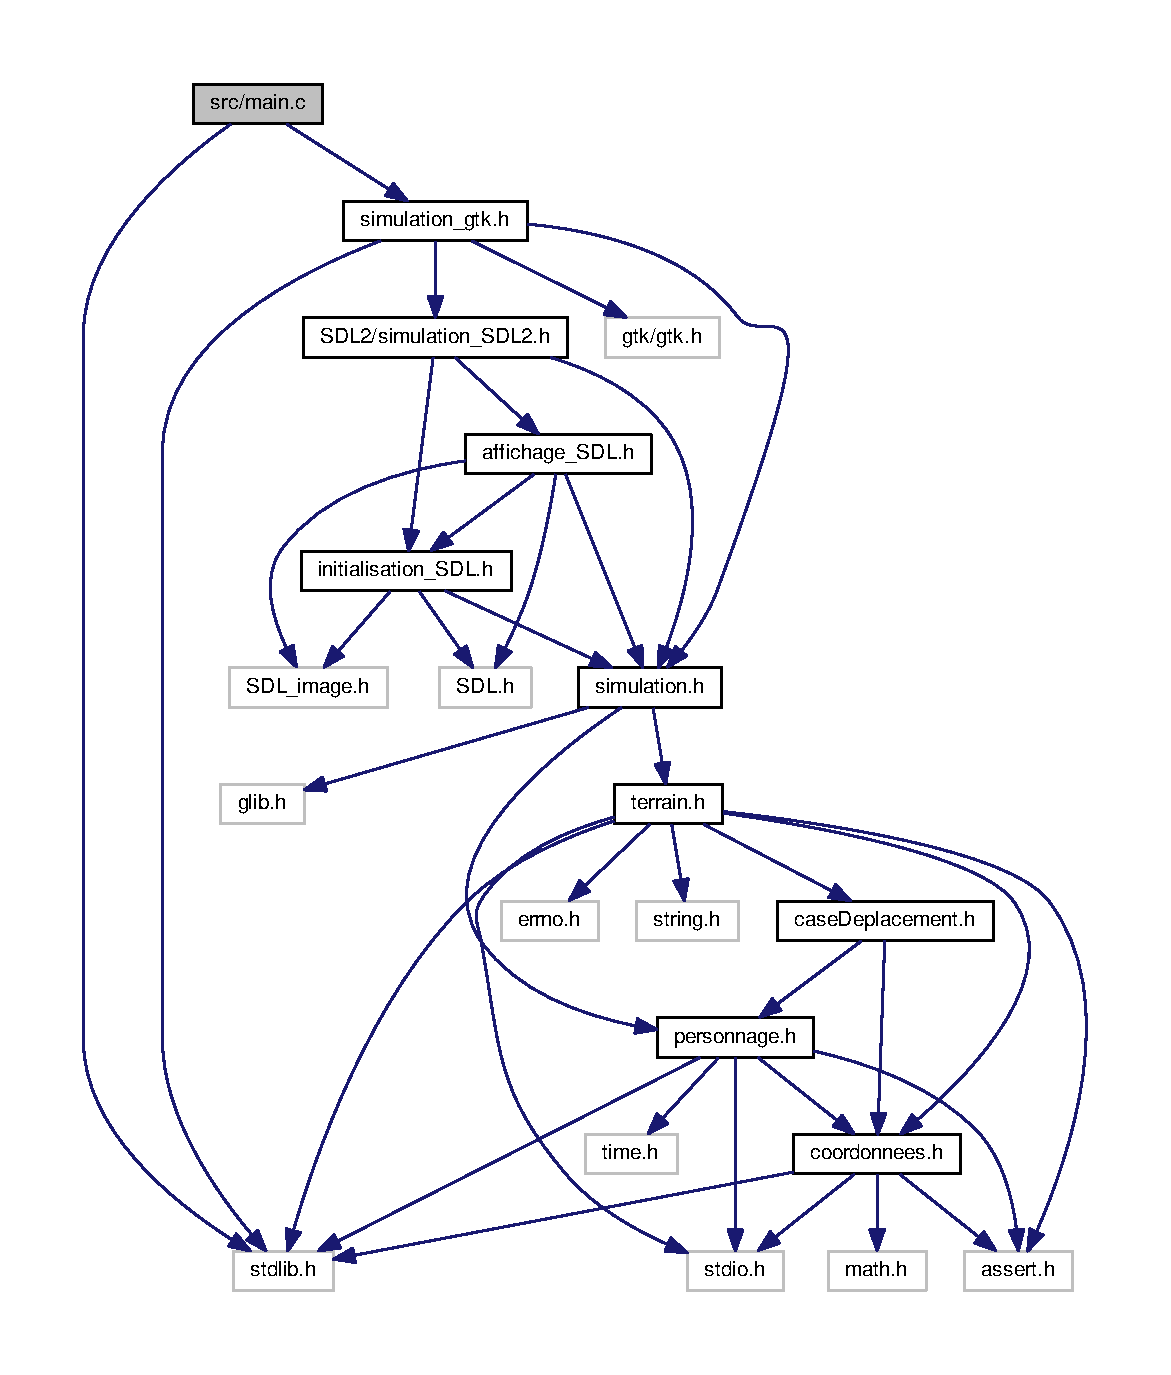
\includegraphics[width=350pt]{main_8c__incl}
\end{center}
\end{figure}
\subsection*{Fonctions}
\begin{DoxyCompactItemize}
\item 
int \hyperlink{main_8c_a3c04138a5bfe5d72780bb7e82a18e627}{main} (int argc, char $\ast$$\ast$argv)
\end{DoxyCompactItemize}


\subsection{Documentation des fonctions}
\index{main.\+c@{main.\+c}!main@{main}}
\index{main@{main}!main.\+c@{main.\+c}}
\subsubsection[{\texorpdfstring{main(int argc, char $\ast$$\ast$argv)}{main(int argc, char **argv)}}]{\setlength{\rightskip}{0pt plus 5cm}int main (
\begin{DoxyParamCaption}
\item[{int}]{argc, }
\item[{char $\ast$$\ast$}]{argv}
\end{DoxyParamCaption}
)}\hypertarget{main_8c_a3c04138a5bfe5d72780bb7e82a18e627}{}\label{main_8c_a3c04138a5bfe5d72780bb7e82a18e627}

\hypertarget{personnage_8c}{}\section{Référence du fichier src/personnage.c}
\label{personnage_8c}\index{src/personnage.\+c@{src/personnage.\+c}}
{\ttfamily \#include \char`\"{}personnage.\+h\char`\"{}}\\*
Graphe des dépendances par inclusion de personnage.\+c\+:
\nopagebreak
\begin{figure}[H]
\begin{center}
\leavevmode
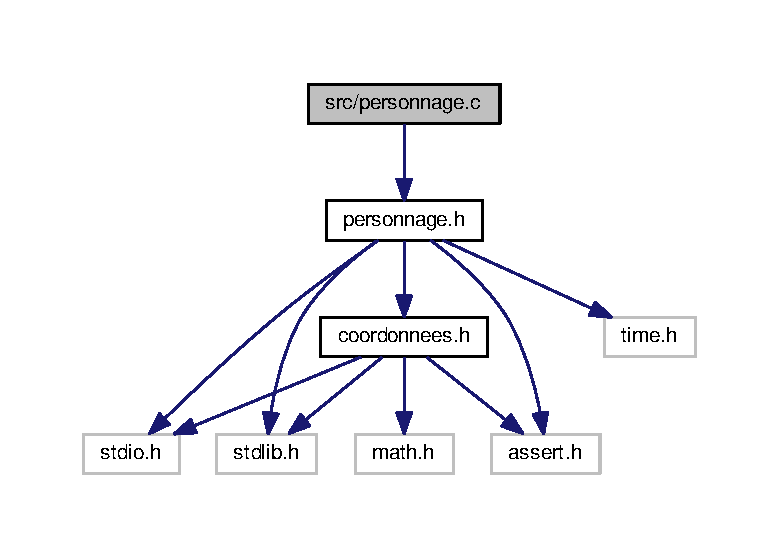
\includegraphics[width=350pt]{personnage_8c__incl}
\end{center}
\end{figure}
\subsection*{Fonctions}
\begin{DoxyCompactItemize}
\item 
\hyperlink{coordonnees_8h_a79929cdfee7bd985a5e4e25276bb3ba9}{Coordonnees} $\ast$ \hyperlink{personnage_8c_a19cfc938b3ee58f313b87e7ca4b62be2}{get\+Coordonnees\+Perso\+\_\+perso} (\hyperlink{personnage_8h_abd5c92a453bbf273f753b3f5b99da9e7}{Perso} $\ast$p\+Perso)
\begin{DoxyCompactList}\small\item\em Retourne des coordonnées d\textquotesingle{}un personnage. \end{DoxyCompactList}\item 
int \hyperlink{personnage_8c_aec9bc09498be7dab178baa5015d97abf}{get\+X\+Perso\+\_\+perso} (\hyperlink{personnage_8h_abd5c92a453bbf273f753b3f5b99da9e7}{Perso} $\ast$p\+Perso)
\begin{DoxyCompactList}\small\item\em Retourne les coordonnées X d\textquotesingle{}un personnage. \end{DoxyCompactList}\item 
int \hyperlink{personnage_8c_aa17a9866dddc2dd8a206364b2b0bcd41}{get\+Y\+Perso\+\_\+perso} (\hyperlink{personnage_8h_abd5c92a453bbf273f753b3f5b99da9e7}{Perso} $\ast$p\+Perso)
\begin{DoxyCompactList}\small\item\em Retourne les coordonnées Y d\textquotesingle{}un personnage. \end{DoxyCompactList}\item 
void \hyperlink{personnage_8c_a68b73c56985831aa9167f26278763b1f}{set\+X\+Perso\+\_\+perso} (\hyperlink{personnage_8h_abd5c92a453bbf273f753b3f5b99da9e7}{Perso} $\ast$p\+Perso, int x\+Perso)
\begin{DoxyCompactList}\small\item\em Change les coordonnées X d\textquotesingle{}un personnage. \end{DoxyCompactList}\item 
void \hyperlink{personnage_8c_ac36bed180c16d77128a18f79fe4afe8d}{set\+Y\+Perso\+\_\+perso} (\hyperlink{personnage_8h_abd5c92a453bbf273f753b3f5b99da9e7}{Perso} $\ast$p\+Perso, int y\+Perso)
\begin{DoxyCompactList}\small\item\em Change les coordonnées Y d\textquotesingle{}un personnage. \end{DoxyCompactList}\item 
void \hyperlink{personnage_8c_ae63f654e86384c7504b289a5e43a0965}{set\+Coord\+Perso\+\_\+perso} (\hyperlink{coordonnees_8h_a79929cdfee7bd985a5e4e25276bb3ba9}{Coordonnees} $\ast$p\+Coord, \hyperlink{personnage_8h_abd5c92a453bbf273f753b3f5b99da9e7}{Perso} $\ast$p\+Perso)
\begin{DoxyCompactList}\small\item\em Change les coordonnées d\textquotesingle{}un personnage. \end{DoxyCompactList}\item 
\hyperlink{coordonnees_8h_a79929cdfee7bd985a5e4e25276bb3ba9}{Coordonnees} $\ast$ \hyperlink{personnage_8c_aa60f8b12745fc87c9010193290c11ef7}{get\+Coord\+Perso} (\hyperlink{personnage_8h_abd5c92a453bbf273f753b3f5b99da9e7}{Perso} $\ast$p\+Perso)
\item 
enum \hyperlink{personnage_8h_a3f6a2951aa3d5d428dd6d61e74db0d75}{type\+Perso} \hyperlink{personnage_8c_ab151e74efaf41694e0ae80d45645b4ae}{get\+Type\+Perso} (\hyperlink{personnage_8h_abd5c92a453bbf273f753b3f5b99da9e7}{Perso} $\ast$p\+Perso)
\begin{DoxyCompactList}\small\item\em Retourne le type de personnage d\textquotesingle{}un perso. \end{DoxyCompactList}\item 
void \hyperlink{personnage_8c_a1bc61d5d213ad2c82a9c6486bb3b6d09}{set\+Type\+Perso\+\_\+perso} (enum \hyperlink{personnage_8h_a3f6a2951aa3d5d428dd6d61e74db0d75}{type\+Perso} \hyperlink{personnage_8h_a3f6a2951aa3d5d428dd6d61e74db0d75}{type\+Perso}, \hyperlink{personnage_8h_abd5c92a453bbf273f753b3f5b99da9e7}{Perso} $\ast$p\+Perso)
\item 
void \hyperlink{personnage_8c_a7ccbdbc540ff48c9bee4e9df01c9e721}{set\+Id\+Perso} (int id\+Perso, \hyperlink{personnage_8h_abd5c92a453bbf273f753b3f5b99da9e7}{Perso} $\ast$p\+Perso)
\begin{DoxyCompactList}\small\item\em Change l\textquotesingle{}Id d\textquotesingle{}un personnage pointé \end{DoxyCompactList}\item 
int \hyperlink{personnage_8c_a52435b6bd9906c613c5de660462639c4}{get\+Id\+Perso} (\hyperlink{personnage_8h_abd5c92a453bbf273f753b3f5b99da9e7}{Perso} $\ast$p\+Perso)
\begin{DoxyCompactList}\small\item\em Retourne l\textquotesingle{}Id d\textquotesingle{}un personnage pointé \end{DoxyCompactList}\item 
\hyperlink{personnage_8h_abd5c92a453bbf273f753b3f5b99da9e7}{Perso} $\ast$ \hyperlink{personnage_8c_a7c7e7effb953fc825ebbe3ed5d362732}{init\+Perso} (\hyperlink{coordonnees_8h_a79929cdfee7bd985a5e4e25276bb3ba9}{Coordonnees} $\ast$p\+Coord, enum \hyperlink{personnage_8h_a3f6a2951aa3d5d428dd6d61e74db0d75}{type\+Perso} \hyperlink{personnage_8h_a3f6a2951aa3d5d428dd6d61e74db0d75}{type\+Perso}, int id\+Perso)
\item 
void \hyperlink{personnage_8c_a2f2cd16139f8de72e55cd99849fea56d}{testament\+Perso} (\hyperlink{personnage_8h_abd5c92a453bbf273f753b3f5b99da9e7}{Perso} $\ast$p\+Perso)
\begin{DoxyCompactList}\small\item\em Detruit le personnage pointé et libère la mémoire. \end{DoxyCompactList}\item 
void \hyperlink{personnage_8c_a722d5ef48f2f08ac15e1a4ab7dfdfe87}{test\+Fonctions\+\_\+perso} ()
\begin{DoxyCompactList}\small\item\em Fontion de test des fonctions du module Personnage. \end{DoxyCompactList}\end{DoxyCompactItemize}


\subsection{Documentation des fonctions}
\index{personnage.\+c@{personnage.\+c}!get\+Coordonnees\+Perso\+\_\+perso@{get\+Coordonnees\+Perso\+\_\+perso}}
\index{get\+Coordonnees\+Perso\+\_\+perso@{get\+Coordonnees\+Perso\+\_\+perso}!personnage.\+c@{personnage.\+c}}
\subsubsection[{\texorpdfstring{get\+Coordonnees\+Perso\+\_\+perso(\+Perso $\ast$p\+Perso)}{getCoordonneesPerso_perso(Perso *pPerso)}}]{\setlength{\rightskip}{0pt plus 5cm}{\bf Coordonnees}$\ast$ get\+Coordonnees\+Perso\+\_\+perso (
\begin{DoxyParamCaption}
\item[{{\bf Perso} $\ast$}]{p\+Perso}
\end{DoxyParamCaption}
)}\hypertarget{personnage_8c_a19cfc938b3ee58f313b87e7ca4b62be2}{}\label{personnage_8c_a19cfc938b3ee58f313b87e7ca4b62be2}


Retourne des coordonnées d\textquotesingle{}un personnage. 


\begin{DoxyParams}{Paramètres}
{\em p\+Perso} & Personnage dont on veut les coordonnées \\
\hline
\end{DoxyParams}
\begin{DoxyReturn}{Renvoie}
Un pointeur vers les coordonnées du personnage 
\end{DoxyReturn}
\index{personnage.\+c@{personnage.\+c}!get\+Coord\+Perso@{get\+Coord\+Perso}}
\index{get\+Coord\+Perso@{get\+Coord\+Perso}!personnage.\+c@{personnage.\+c}}
\subsubsection[{\texorpdfstring{get\+Coord\+Perso(\+Perso $\ast$p\+Perso)}{getCoordPerso(Perso *pPerso)}}]{\setlength{\rightskip}{0pt plus 5cm}{\bf Coordonnees}$\ast$ get\+Coord\+Perso (
\begin{DoxyParamCaption}
\item[{{\bf Perso} $\ast$}]{p\+Perso}
\end{DoxyParamCaption}
)}\hypertarget{personnage_8c_aa60f8b12745fc87c9010193290c11ef7}{}\label{personnage_8c_aa60f8b12745fc87c9010193290c11ef7}
\index{personnage.\+c@{personnage.\+c}!get\+Id\+Perso@{get\+Id\+Perso}}
\index{get\+Id\+Perso@{get\+Id\+Perso}!personnage.\+c@{personnage.\+c}}
\subsubsection[{\texorpdfstring{get\+Id\+Perso(\+Perso $\ast$p\+Perso)}{getIdPerso(Perso *pPerso)}}]{\setlength{\rightskip}{0pt plus 5cm}int get\+Id\+Perso (
\begin{DoxyParamCaption}
\item[{{\bf Perso} $\ast$}]{p\+Perso}
\end{DoxyParamCaption}
)}\hypertarget{personnage_8c_a52435b6bd9906c613c5de660462639c4}{}\label{personnage_8c_a52435b6bd9906c613c5de660462639c4}


Retourne l\textquotesingle{}Id d\textquotesingle{}un personnage pointé 


\begin{DoxyParams}{Paramètres}
{\em p\+Perso} & Le personnage dont on veut l\textquotesingle{}ID \\
\hline
\end{DoxyParams}
\begin{DoxyReturn}{Renvoie}
L\textquotesingle{}ID sous forme d\textquotesingle{}entier 
\end{DoxyReturn}
\index{personnage.\+c@{personnage.\+c}!get\+Type\+Perso@{get\+Type\+Perso}}
\index{get\+Type\+Perso@{get\+Type\+Perso}!personnage.\+c@{personnage.\+c}}
\subsubsection[{\texorpdfstring{get\+Type\+Perso(\+Perso $\ast$p\+Perso)}{getTypePerso(Perso *pPerso)}}]{\setlength{\rightskip}{0pt plus 5cm}enum {\bf type\+Perso} get\+Type\+Perso (
\begin{DoxyParamCaption}
\item[{{\bf Perso} $\ast$}]{p\+Perso}
\end{DoxyParamCaption}
)}\hypertarget{personnage_8c_ab151e74efaf41694e0ae80d45645b4ae}{}\label{personnage_8c_ab151e74efaf41694e0ae80d45645b4ae}


Retourne le type de personnage d\textquotesingle{}un perso. 


\begin{DoxyParams}{Paramètres}
{\em p\+Perso} & Personnage dont on veut le type \\
\hline
\end{DoxyParams}
\begin{DoxyReturn}{Renvoie}
Un enum qui dit le type du perso (zombie, citoyen, policier) 
\end{DoxyReturn}
\index{personnage.\+c@{personnage.\+c}!get\+X\+Perso\+\_\+perso@{get\+X\+Perso\+\_\+perso}}
\index{get\+X\+Perso\+\_\+perso@{get\+X\+Perso\+\_\+perso}!personnage.\+c@{personnage.\+c}}
\subsubsection[{\texorpdfstring{get\+X\+Perso\+\_\+perso(\+Perso $\ast$p\+Perso)}{getXPerso_perso(Perso *pPerso)}}]{\setlength{\rightskip}{0pt plus 5cm}int get\+X\+Perso\+\_\+perso (
\begin{DoxyParamCaption}
\item[{{\bf Perso} $\ast$}]{p\+Perso}
\end{DoxyParamCaption}
)}\hypertarget{personnage_8c_aec9bc09498be7dab178baa5015d97abf}{}\label{personnage_8c_aec9bc09498be7dab178baa5015d97abf}


Retourne les coordonnées X d\textquotesingle{}un personnage. 


\begin{DoxyParams}{Paramètres}
{\em p\+Perso} & Personnage dont on veut les coordonnées \\
\hline
\end{DoxyParams}
\begin{DoxyReturn}{Renvoie}
Un entier des coordonnées en X 
\end{DoxyReturn}
\index{personnage.\+c@{personnage.\+c}!get\+Y\+Perso\+\_\+perso@{get\+Y\+Perso\+\_\+perso}}
\index{get\+Y\+Perso\+\_\+perso@{get\+Y\+Perso\+\_\+perso}!personnage.\+c@{personnage.\+c}}
\subsubsection[{\texorpdfstring{get\+Y\+Perso\+\_\+perso(\+Perso $\ast$p\+Perso)}{getYPerso_perso(Perso *pPerso)}}]{\setlength{\rightskip}{0pt plus 5cm}int get\+Y\+Perso\+\_\+perso (
\begin{DoxyParamCaption}
\item[{{\bf Perso} $\ast$}]{p\+Perso}
\end{DoxyParamCaption}
)}\hypertarget{personnage_8c_aa17a9866dddc2dd8a206364b2b0bcd41}{}\label{personnage_8c_aa17a9866dddc2dd8a206364b2b0bcd41}


Retourne les coordonnées Y d\textquotesingle{}un personnage. 


\begin{DoxyParams}{Paramètres}
{\em p\+Perso} & Personnage dont on veut les coordonnées \\
\hline
\end{DoxyParams}
\begin{DoxyReturn}{Renvoie}
Un entier des coordonnées en Y 
\end{DoxyReturn}
\index{personnage.\+c@{personnage.\+c}!init\+Perso@{init\+Perso}}
\index{init\+Perso@{init\+Perso}!personnage.\+c@{personnage.\+c}}
\subsubsection[{\texorpdfstring{init\+Perso(\+Coordonnees $\ast$p\+Coord, enum type\+Perso type\+Perso, int id\+Perso)}{initPerso(Coordonnees *pCoord, enum typePerso typePerso, int idPerso)}}]{\setlength{\rightskip}{0pt plus 5cm}{\bf Perso}$\ast$ init\+Perso (
\begin{DoxyParamCaption}
\item[{{\bf Coordonnees} $\ast$}]{p\+Coord, }
\item[{enum {\bf type\+Perso} {\bf type\+Perso}}]{, }
\item[{int}]{id\+Perso}
\end{DoxyParamCaption}
)}\hypertarget{personnage_8c_a7c7e7effb953fc825ebbe3ed5d362732}{}\label{personnage_8c_a7c7e7effb953fc825ebbe3ed5d362732}
\index{personnage.\+c@{personnage.\+c}!set\+Coord\+Perso\+\_\+perso@{set\+Coord\+Perso\+\_\+perso}}
\index{set\+Coord\+Perso\+\_\+perso@{set\+Coord\+Perso\+\_\+perso}!personnage.\+c@{personnage.\+c}}
\subsubsection[{\texorpdfstring{set\+Coord\+Perso\+\_\+perso(\+Coordonnees $\ast$p\+Coord, Perso $\ast$p\+Perso)}{setCoordPerso_perso(Coordonnees *pCoord, Perso *pPerso)}}]{\setlength{\rightskip}{0pt plus 5cm}void set\+Coord\+Perso\+\_\+perso (
\begin{DoxyParamCaption}
\item[{{\bf Coordonnees} $\ast$}]{p\+Coord, }
\item[{{\bf Perso} $\ast$}]{p\+Perso}
\end{DoxyParamCaption}
)}\hypertarget{personnage_8c_ae63f654e86384c7504b289a5e43a0965}{}\label{personnage_8c_ae63f654e86384c7504b289a5e43a0965}


Change les coordonnées d\textquotesingle{}un personnage. 


\begin{DoxyParams}{Paramètres}
{\em p\+Coord} & Pointeur vers des coordonnées \\
\hline
{\em p\+Perso} & Personnage dont on veut changer les coordonnées \\
\hline
\end{DoxyParams}
\index{personnage.\+c@{personnage.\+c}!set\+Id\+Perso@{set\+Id\+Perso}}
\index{set\+Id\+Perso@{set\+Id\+Perso}!personnage.\+c@{personnage.\+c}}
\subsubsection[{\texorpdfstring{set\+Id\+Perso(int id\+Perso, Perso $\ast$p\+Perso)}{setIdPerso(int idPerso, Perso *pPerso)}}]{\setlength{\rightskip}{0pt plus 5cm}void set\+Id\+Perso (
\begin{DoxyParamCaption}
\item[{int}]{id\+Perso, }
\item[{{\bf Perso} $\ast$}]{p\+Perso}
\end{DoxyParamCaption}
)}\hypertarget{personnage_8c_a7ccbdbc540ff48c9bee4e9df01c9e721}{}\label{personnage_8c_a7ccbdbc540ff48c9bee4e9df01c9e721}


Change l\textquotesingle{}Id d\textquotesingle{}un personnage pointé 


\begin{DoxyParams}{Paramètres}
{\em id\+Perso} & L\textquotesingle{}ID sous forme d\textquotesingle{}entier \\
\hline
{\em p\+Perso} & Le personnage dont on veut l\textquotesingle{}ID \\
\hline
\end{DoxyParams}
\index{personnage.\+c@{personnage.\+c}!set\+Type\+Perso\+\_\+perso@{set\+Type\+Perso\+\_\+perso}}
\index{set\+Type\+Perso\+\_\+perso@{set\+Type\+Perso\+\_\+perso}!personnage.\+c@{personnage.\+c}}
\subsubsection[{\texorpdfstring{set\+Type\+Perso\+\_\+perso(enum type\+Perso type\+Perso, Perso $\ast$p\+Perso)}{setTypePerso_perso(enum typePerso typePerso, Perso *pPerso)}}]{\setlength{\rightskip}{0pt plus 5cm}void set\+Type\+Perso\+\_\+perso (
\begin{DoxyParamCaption}
\item[{enum {\bf type\+Perso} {\bf type\+Perso}}]{, }
\item[{{\bf Perso} $\ast$}]{p\+Perso}
\end{DoxyParamCaption}
)}\hypertarget{personnage_8c_a1bc61d5d213ad2c82a9c6486bb3b6d09}{}\label{personnage_8c_a1bc61d5d213ad2c82a9c6486bb3b6d09}
\index{personnage.\+c@{personnage.\+c}!set\+X\+Perso\+\_\+perso@{set\+X\+Perso\+\_\+perso}}
\index{set\+X\+Perso\+\_\+perso@{set\+X\+Perso\+\_\+perso}!personnage.\+c@{personnage.\+c}}
\subsubsection[{\texorpdfstring{set\+X\+Perso\+\_\+perso(\+Perso $\ast$p\+Perso, int x\+Perso)}{setXPerso_perso(Perso *pPerso, int xPerso)}}]{\setlength{\rightskip}{0pt plus 5cm}void set\+X\+Perso\+\_\+perso (
\begin{DoxyParamCaption}
\item[{{\bf Perso} $\ast$}]{p\+Perso, }
\item[{int}]{x\+Perso}
\end{DoxyParamCaption}
)}\hypertarget{personnage_8c_a68b73c56985831aa9167f26278763b1f}{}\label{personnage_8c_a68b73c56985831aa9167f26278763b1f}


Change les coordonnées X d\textquotesingle{}un personnage. 


\begin{DoxyParams}{Paramètres}
{\em p\+Perso} & Personnage dont on veut changer les coordonnées \\
\hline
{\em x\+Perso} & Un entier des coordonnées en X à changer \\
\hline
\end{DoxyParams}
\index{personnage.\+c@{personnage.\+c}!set\+Y\+Perso\+\_\+perso@{set\+Y\+Perso\+\_\+perso}}
\index{set\+Y\+Perso\+\_\+perso@{set\+Y\+Perso\+\_\+perso}!personnage.\+c@{personnage.\+c}}
\subsubsection[{\texorpdfstring{set\+Y\+Perso\+\_\+perso(\+Perso $\ast$p\+Perso, int y\+Perso)}{setYPerso_perso(Perso *pPerso, int yPerso)}}]{\setlength{\rightskip}{0pt plus 5cm}void set\+Y\+Perso\+\_\+perso (
\begin{DoxyParamCaption}
\item[{{\bf Perso} $\ast$}]{p\+Perso, }
\item[{int}]{y\+Perso}
\end{DoxyParamCaption}
)}\hypertarget{personnage_8c_ac36bed180c16d77128a18f79fe4afe8d}{}\label{personnage_8c_ac36bed180c16d77128a18f79fe4afe8d}


Change les coordonnées Y d\textquotesingle{}un personnage. 


\begin{DoxyParams}{Paramètres}
{\em p\+Perso} & Personnage dont on veut changer les coordonnées \\
\hline
{\em y\+Perso} & Un entier des coordonnées en Y à changer \\
\hline
\end{DoxyParams}
\index{personnage.\+c@{personnage.\+c}!testament\+Perso@{testament\+Perso}}
\index{testament\+Perso@{testament\+Perso}!personnage.\+c@{personnage.\+c}}
\subsubsection[{\texorpdfstring{testament\+Perso(\+Perso $\ast$p\+Perso)}{testamentPerso(Perso *pPerso)}}]{\setlength{\rightskip}{0pt plus 5cm}void testament\+Perso (
\begin{DoxyParamCaption}
\item[{{\bf Perso} $\ast$}]{p\+Perso}
\end{DoxyParamCaption}
)}\hypertarget{personnage_8c_a2f2cd16139f8de72e55cd99849fea56d}{}\label{personnage_8c_a2f2cd16139f8de72e55cd99849fea56d}


Detruit le personnage pointé et libère la mémoire. 


\begin{DoxyParams}{Paramètres}
{\em p\+Perso} & Pointeur vers le personnage a détruire et liberer \\
\hline
\end{DoxyParams}
\index{personnage.\+c@{personnage.\+c}!test\+Fonctions\+\_\+perso@{test\+Fonctions\+\_\+perso}}
\index{test\+Fonctions\+\_\+perso@{test\+Fonctions\+\_\+perso}!personnage.\+c@{personnage.\+c}}
\subsubsection[{\texorpdfstring{test\+Fonctions\+\_\+perso()}{testFonctions_perso()}}]{\setlength{\rightskip}{0pt plus 5cm}void test\+Fonctions\+\_\+perso (
\begin{DoxyParamCaption}
{}
\end{DoxyParamCaption}
)}\hypertarget{personnage_8c_a722d5ef48f2f08ac15e1a4ab7dfdfe87}{}\label{personnage_8c_a722d5ef48f2f08ac15e1a4ab7dfdfe87}


Fontion de test des fonctions du module Personnage. 


\hypertarget{personnage_8h}{}\section{Référence du fichier src/personnage.h}
\label{personnage_8h}\index{src/personnage.\+h@{src/personnage.\+h}}


Définit les type de personnage et leurs accesseurs.  


{\ttfamily \#include \char`\"{}coordonnees.\+h\char`\"{}}\\*
{\ttfamily \#include \char`\"{}assert.\+h\char`\"{}}\\*
{\ttfamily \#include \char`\"{}time.\+h\char`\"{}}\\*
{\ttfamily \#include $<$stdlib.\+h$>$}\\*
{\ttfamily \#include $<$stdio.\+h$>$}\\*
Graphe des dépendances par inclusion de personnage.\+h\+:\nopagebreak
\begin{figure}[H]
\begin{center}
\leavevmode
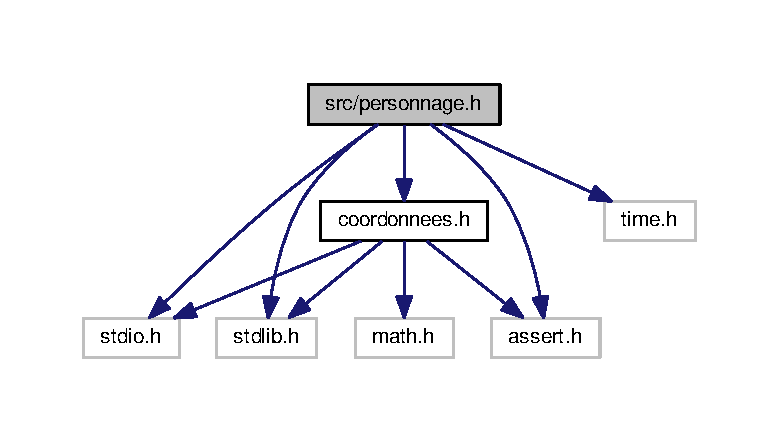
\includegraphics[width=350pt]{personnage_8h__incl}
\end{center}
\end{figure}
Ce graphe montre quels fichiers incluent directement ou indirectement ce fichier \+:\nopagebreak
\begin{figure}[H]
\begin{center}
\leavevmode
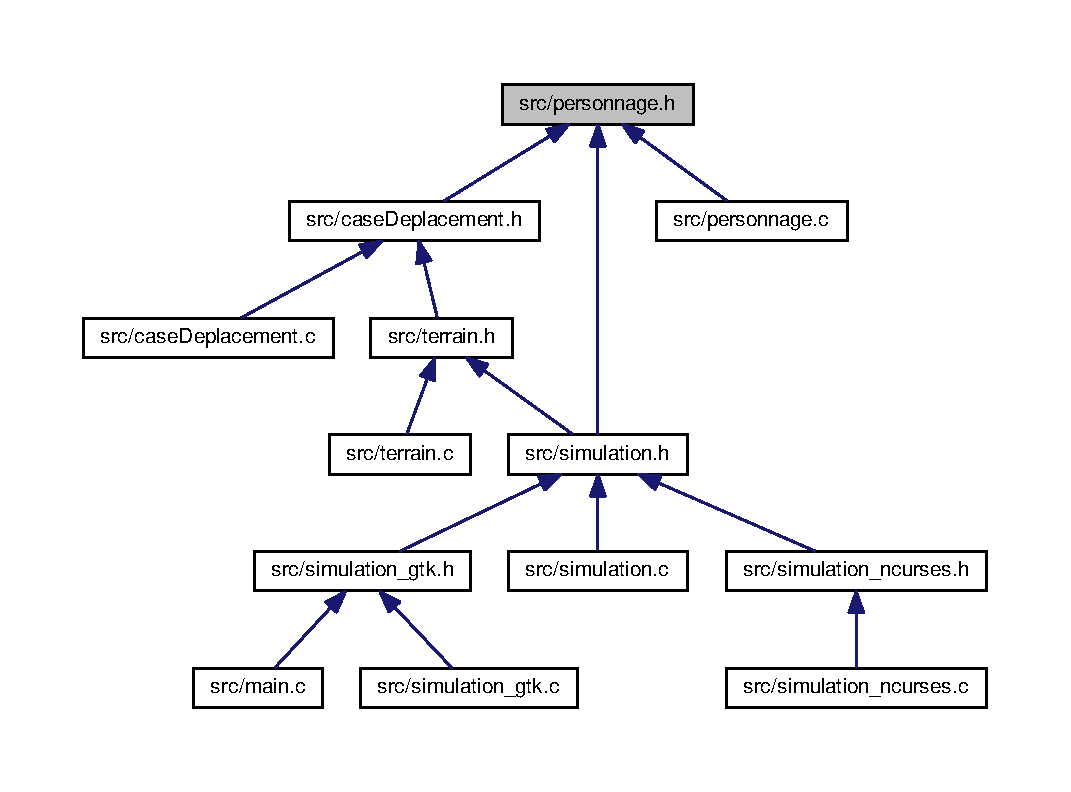
\includegraphics[width=350pt]{personnage_8h__dep__incl}
\end{center}
\end{figure}
\subsection*{Classes}
\begin{DoxyCompactItemize}
\item 
struct \hyperlink{structMPerso}{M\+Perso}
\begin{DoxyCompactList}\small\item\em Structure definissant un personnage et ses attributs. \end{DoxyCompactList}\end{DoxyCompactItemize}
\subsection*{Définitions de type}
\begin{DoxyCompactItemize}
\item 
typedef struct \hyperlink{structMPerso}{M\+Perso} \hyperlink{personnage_8h_abd5c92a453bbf273f753b3f5b99da9e7}{Perso}
\end{DoxyCompactItemize}
\subsection*{Énumérations}
\begin{DoxyCompactItemize}
\item 
enum \hyperlink{personnage_8h_a3f6a2951aa3d5d428dd6d61e74db0d75}{type\+Perso} \{ \hyperlink{personnage_8h_a3f6a2951aa3d5d428dd6d61e74db0d75a1db595a33d341b53fbd208d9cce5d0fc}{P\+O\+L\+I\+C\+I\+ER}, 
\hyperlink{personnage_8h_a3f6a2951aa3d5d428dd6d61e74db0d75a5dfb36109b24f39d54d5c3f48f53def8}{Z\+O\+M\+B\+IE}, 
\hyperlink{personnage_8h_a3f6a2951aa3d5d428dd6d61e74db0d75aea28a2bbfeeafa3a7de5daa12914e76b}{C\+I\+T\+O\+Y\+EN}
 \}
\end{DoxyCompactItemize}
\subsection*{Fonctions}
\begin{DoxyCompactItemize}
\item 
\hyperlink{coordonnees_8h_a79929cdfee7bd985a5e4e25276bb3ba9}{Coordonnees} $\ast$ \hyperlink{personnage_8h_a19cfc938b3ee58f313b87e7ca4b62be2}{get\+Coordonnees\+Perso\+\_\+perso} (\hyperlink{personnage_8h_abd5c92a453bbf273f753b3f5b99da9e7}{Perso} $\ast$p\+Perso)
\begin{DoxyCompactList}\small\item\em Retourne des coordonnées d\textquotesingle{}un personnage. \end{DoxyCompactList}\item 
int \hyperlink{personnage_8h_aec9bc09498be7dab178baa5015d97abf}{get\+X\+Perso\+\_\+perso} (\hyperlink{personnage_8h_abd5c92a453bbf273f753b3f5b99da9e7}{Perso} $\ast$p\+Perso)
\begin{DoxyCompactList}\small\item\em Retourne les coordonnées X d\textquotesingle{}un personnage. \end{DoxyCompactList}\item 
int \hyperlink{personnage_8h_aa17a9866dddc2dd8a206364b2b0bcd41}{get\+Y\+Perso\+\_\+perso} (\hyperlink{personnage_8h_abd5c92a453bbf273f753b3f5b99da9e7}{Perso} $\ast$p\+Perso)
\begin{DoxyCompactList}\small\item\em Retourne les coordonnées Y d\textquotesingle{}un personnage. \end{DoxyCompactList}\item 
void \hyperlink{personnage_8h_a68b73c56985831aa9167f26278763b1f}{set\+X\+Perso\+\_\+perso} (\hyperlink{personnage_8h_abd5c92a453bbf273f753b3f5b99da9e7}{Perso} $\ast$p\+Perso, int x\+Perso)
\begin{DoxyCompactList}\small\item\em Change les coordonnées X d\textquotesingle{}un personnage. \end{DoxyCompactList}\item 
void \hyperlink{personnage_8h_ac36bed180c16d77128a18f79fe4afe8d}{set\+Y\+Perso\+\_\+perso} (\hyperlink{personnage_8h_abd5c92a453bbf273f753b3f5b99da9e7}{Perso} $\ast$p\+Perso, int y\+Perso)
\begin{DoxyCompactList}\small\item\em Change les coordonnées Y d\textquotesingle{}un personnage. \end{DoxyCompactList}\item 
\hyperlink{coordonnees_8h_a79929cdfee7bd985a5e4e25276bb3ba9}{Coordonnees} $\ast$ \hyperlink{personnage_8h_aa60f8b12745fc87c9010193290c11ef7}{get\+Coord\+Perso} (\hyperlink{personnage_8h_abd5c92a453bbf273f753b3f5b99da9e7}{Perso} $\ast$p\+Perso)
\item 
enum \hyperlink{personnage_8h_a3f6a2951aa3d5d428dd6d61e74db0d75}{type\+Perso} \hyperlink{personnage_8h_ab151e74efaf41694e0ae80d45645b4ae}{get\+Type\+Perso} (\hyperlink{personnage_8h_abd5c92a453bbf273f753b3f5b99da9e7}{Perso} $\ast$p\+Perso)
\begin{DoxyCompactList}\small\item\em Retourne le type de personnage d\textquotesingle{}un perso. \end{DoxyCompactList}\item 
void \hyperlink{personnage_8h_ac14e27d8d05362bd811de08b2b73519e}{set\+Type\+Perso\+\_\+perso} (enum \hyperlink{personnage_8h_a3f6a2951aa3d5d428dd6d61e74db0d75}{type\+Perso} type, \hyperlink{personnage_8h_abd5c92a453bbf273f753b3f5b99da9e7}{Perso} $\ast$p\+Perso)
\begin{DoxyCompactList}\small\item\em Change le type de personnage d\textquotesingle{}un perso. \end{DoxyCompactList}\item 
void \hyperlink{personnage_8h_ae63f654e86384c7504b289a5e43a0965}{set\+Coord\+Perso\+\_\+perso} (\hyperlink{coordonnees_8h_a79929cdfee7bd985a5e4e25276bb3ba9}{Coordonnees} $\ast$p\+Coord, \hyperlink{personnage_8h_abd5c92a453bbf273f753b3f5b99da9e7}{Perso} $\ast$p\+Perso)
\begin{DoxyCompactList}\small\item\em Change les coordonnées d\textquotesingle{}un personnage. \end{DoxyCompactList}\item 
int \hyperlink{personnage_8h_a52435b6bd9906c613c5de660462639c4}{get\+Id\+Perso} (\hyperlink{personnage_8h_abd5c92a453bbf273f753b3f5b99da9e7}{Perso} $\ast$p\+Perso)
\begin{DoxyCompactList}\small\item\em Retourne l\textquotesingle{}Id d\textquotesingle{}un personnage pointé \end{DoxyCompactList}\item 
void \hyperlink{personnage_8h_a7ccbdbc540ff48c9bee4e9df01c9e721}{set\+Id\+Perso} (int id\+Perso, \hyperlink{personnage_8h_abd5c92a453bbf273f753b3f5b99da9e7}{Perso} $\ast$p\+Perso)
\begin{DoxyCompactList}\small\item\em Change l\textquotesingle{}Id d\textquotesingle{}un personnage pointé \end{DoxyCompactList}\item 
\hyperlink{personnage_8h_abd5c92a453bbf273f753b3f5b99da9e7}{Perso} $\ast$ \hyperlink{personnage_8h_a285ef94e77a694361718b2bd7c9f32c5}{init\+Perso} (\hyperlink{coordonnees_8h_a79929cdfee7bd985a5e4e25276bb3ba9}{Coordonnees} $\ast$p\+Coord, enum \hyperlink{personnage_8h_a3f6a2951aa3d5d428dd6d61e74db0d75}{type\+Perso} type, int id\+Perso)
\begin{DoxyCompactList}\small\item\em Créer et initialise un personnage et renvoie un pointeur vers lui. \end{DoxyCompactList}\item 
void \hyperlink{personnage_8h_a2f2cd16139f8de72e55cd99849fea56d}{testament\+Perso} (\hyperlink{personnage_8h_abd5c92a453bbf273f753b3f5b99da9e7}{Perso} $\ast$p\+Perso)
\begin{DoxyCompactList}\small\item\em Detruit le personnage pointé et libère la mémoire. \end{DoxyCompactList}\item 
void \hyperlink{personnage_8h_a722d5ef48f2f08ac15e1a4ab7dfdfe87}{test\+Fonctions\+\_\+perso} ()
\begin{DoxyCompactList}\small\item\em Fontion de test des fonctions du module Personnage. \end{DoxyCompactList}\end{DoxyCompactItemize}


\subsection{Description détaillée}
Définit les type de personnage et leurs accesseurs. 



\subsection{Documentation des définitions de type}
\index{personnage.\+h@{personnage.\+h}!Perso@{Perso}}
\index{Perso@{Perso}!personnage.\+h@{personnage.\+h}}
\subsubsection[{\texorpdfstring{Perso}{Perso}}]{\setlength{\rightskip}{0pt plus 5cm}typedef struct {\bf M\+Perso}  {\bf Perso}}\hypertarget{personnage_8h_abd5c92a453bbf273f753b3f5b99da9e7}{}\label{personnage_8h_abd5c92a453bbf273f753b3f5b99da9e7}


\subsection{Documentation du type de l\textquotesingle{}énumération}
\index{personnage.\+h@{personnage.\+h}!type\+Perso@{type\+Perso}}
\index{type\+Perso@{type\+Perso}!personnage.\+h@{personnage.\+h}}
\subsubsection[{\texorpdfstring{type\+Perso}{typePerso}}]{\setlength{\rightskip}{0pt plus 5cm}enum {\bf type\+Perso}}\hypertarget{personnage_8h_a3f6a2951aa3d5d428dd6d61e74db0d75}{}\label{personnage_8h_a3f6a2951aa3d5d428dd6d61e74db0d75}
Les différents type de personnages \begin{Desc}
\item[Valeurs énumérées]\par
\begin{description}
\index{P\+O\+L\+I\+C\+I\+ER@{P\+O\+L\+I\+C\+I\+ER}!personnage.\+h@{personnage.\+h}}\index{personnage.\+h@{personnage.\+h}!P\+O\+L\+I\+C\+I\+ER@{P\+O\+L\+I\+C\+I\+ER}}\item[{\em 
P\+O\+L\+I\+C\+I\+ER\hypertarget{personnage_8h_a3f6a2951aa3d5d428dd6d61e74db0d75a1db595a33d341b53fbd208d9cce5d0fc}{}\label{personnage_8h_a3f6a2951aa3d5d428dd6d61e74db0d75a1db595a33d341b53fbd208d9cce5d0fc}
}]\index{Z\+O\+M\+B\+IE@{Z\+O\+M\+B\+IE}!personnage.\+h@{personnage.\+h}}\index{personnage.\+h@{personnage.\+h}!Z\+O\+M\+B\+IE@{Z\+O\+M\+B\+IE}}\item[{\em 
Z\+O\+M\+B\+IE\hypertarget{personnage_8h_a3f6a2951aa3d5d428dd6d61e74db0d75a5dfb36109b24f39d54d5c3f48f53def8}{}\label{personnage_8h_a3f6a2951aa3d5d428dd6d61e74db0d75a5dfb36109b24f39d54d5c3f48f53def8}
}]\index{C\+I\+T\+O\+Y\+EN@{C\+I\+T\+O\+Y\+EN}!personnage.\+h@{personnage.\+h}}\index{personnage.\+h@{personnage.\+h}!C\+I\+T\+O\+Y\+EN@{C\+I\+T\+O\+Y\+EN}}\item[{\em 
C\+I\+T\+O\+Y\+EN\hypertarget{personnage_8h_a3f6a2951aa3d5d428dd6d61e74db0d75aea28a2bbfeeafa3a7de5daa12914e76b}{}\label{personnage_8h_a3f6a2951aa3d5d428dd6d61e74db0d75aea28a2bbfeeafa3a7de5daa12914e76b}
}]\end{description}
\end{Desc}


\subsection{Documentation des fonctions}
\index{personnage.\+h@{personnage.\+h}!get\+Coordonnees\+Perso\+\_\+perso@{get\+Coordonnees\+Perso\+\_\+perso}}
\index{get\+Coordonnees\+Perso\+\_\+perso@{get\+Coordonnees\+Perso\+\_\+perso}!personnage.\+h@{personnage.\+h}}
\subsubsection[{\texorpdfstring{get\+Coordonnees\+Perso\+\_\+perso(\+Perso $\ast$p\+Perso)}{getCoordonneesPerso_perso(Perso *pPerso)}}]{\setlength{\rightskip}{0pt plus 5cm}{\bf Coordonnees}$\ast$ get\+Coordonnees\+Perso\+\_\+perso (
\begin{DoxyParamCaption}
\item[{{\bf Perso} $\ast$}]{p\+Perso}
\end{DoxyParamCaption}
)}\hypertarget{personnage_8h_a19cfc938b3ee58f313b87e7ca4b62be2}{}\label{personnage_8h_a19cfc938b3ee58f313b87e7ca4b62be2}


Retourne des coordonnées d\textquotesingle{}un personnage. 


\begin{DoxyParams}{Paramètres}
{\em p\+Perso} & Personnage dont on veut les coordonnées \\
\hline
\end{DoxyParams}
\begin{DoxyReturn}{Renvoie}
Un pointeur vers les coordonnées du personnage 
\end{DoxyReturn}
\index{personnage.\+h@{personnage.\+h}!get\+Coord\+Perso@{get\+Coord\+Perso}}
\index{get\+Coord\+Perso@{get\+Coord\+Perso}!personnage.\+h@{personnage.\+h}}
\subsubsection[{\texorpdfstring{get\+Coord\+Perso(\+Perso $\ast$p\+Perso)}{getCoordPerso(Perso *pPerso)}}]{\setlength{\rightskip}{0pt plus 5cm}{\bf Coordonnees}$\ast$ get\+Coord\+Perso (
\begin{DoxyParamCaption}
\item[{{\bf Perso} $\ast$}]{p\+Perso}
\end{DoxyParamCaption}
)}\hypertarget{personnage_8h_aa60f8b12745fc87c9010193290c11ef7}{}\label{personnage_8h_aa60f8b12745fc87c9010193290c11ef7}
\index{personnage.\+h@{personnage.\+h}!get\+Id\+Perso@{get\+Id\+Perso}}
\index{get\+Id\+Perso@{get\+Id\+Perso}!personnage.\+h@{personnage.\+h}}
\subsubsection[{\texorpdfstring{get\+Id\+Perso(\+Perso $\ast$p\+Perso)}{getIdPerso(Perso *pPerso)}}]{\setlength{\rightskip}{0pt plus 5cm}int get\+Id\+Perso (
\begin{DoxyParamCaption}
\item[{{\bf Perso} $\ast$}]{p\+Perso}
\end{DoxyParamCaption}
)}\hypertarget{personnage_8h_a52435b6bd9906c613c5de660462639c4}{}\label{personnage_8h_a52435b6bd9906c613c5de660462639c4}


Retourne l\textquotesingle{}Id d\textquotesingle{}un personnage pointé 


\begin{DoxyParams}{Paramètres}
{\em p\+Perso} & Le personnage dont on veut l\textquotesingle{}ID \\
\hline
\end{DoxyParams}
\begin{DoxyReturn}{Renvoie}
L\textquotesingle{}ID sous forme d\textquotesingle{}entier 
\end{DoxyReturn}
\index{personnage.\+h@{personnage.\+h}!get\+Type\+Perso@{get\+Type\+Perso}}
\index{get\+Type\+Perso@{get\+Type\+Perso}!personnage.\+h@{personnage.\+h}}
\subsubsection[{\texorpdfstring{get\+Type\+Perso(\+Perso $\ast$p\+Perso)}{getTypePerso(Perso *pPerso)}}]{\setlength{\rightskip}{0pt plus 5cm}enum {\bf type\+Perso} get\+Type\+Perso (
\begin{DoxyParamCaption}
\item[{{\bf Perso} $\ast$}]{p\+Perso}
\end{DoxyParamCaption}
)}\hypertarget{personnage_8h_ab151e74efaf41694e0ae80d45645b4ae}{}\label{personnage_8h_ab151e74efaf41694e0ae80d45645b4ae}


Retourne le type de personnage d\textquotesingle{}un perso. 


\begin{DoxyParams}{Paramètres}
{\em p\+Perso} & Personnage dont on veut le type \\
\hline
\end{DoxyParams}
\begin{DoxyReturn}{Renvoie}
Un enum qui dit le type du perso (zombie, citoyen, policier) 
\end{DoxyReturn}
\index{personnage.\+h@{personnage.\+h}!get\+X\+Perso\+\_\+perso@{get\+X\+Perso\+\_\+perso}}
\index{get\+X\+Perso\+\_\+perso@{get\+X\+Perso\+\_\+perso}!personnage.\+h@{personnage.\+h}}
\subsubsection[{\texorpdfstring{get\+X\+Perso\+\_\+perso(\+Perso $\ast$p\+Perso)}{getXPerso_perso(Perso *pPerso)}}]{\setlength{\rightskip}{0pt plus 5cm}int get\+X\+Perso\+\_\+perso (
\begin{DoxyParamCaption}
\item[{{\bf Perso} $\ast$}]{p\+Perso}
\end{DoxyParamCaption}
)}\hypertarget{personnage_8h_aec9bc09498be7dab178baa5015d97abf}{}\label{personnage_8h_aec9bc09498be7dab178baa5015d97abf}


Retourne les coordonnées X d\textquotesingle{}un personnage. 


\begin{DoxyParams}{Paramètres}
{\em p\+Perso} & Personnage dont on veut les coordonnées \\
\hline
\end{DoxyParams}
\begin{DoxyReturn}{Renvoie}
Un entier des coordonnées en X 
\end{DoxyReturn}
\index{personnage.\+h@{personnage.\+h}!get\+Y\+Perso\+\_\+perso@{get\+Y\+Perso\+\_\+perso}}
\index{get\+Y\+Perso\+\_\+perso@{get\+Y\+Perso\+\_\+perso}!personnage.\+h@{personnage.\+h}}
\subsubsection[{\texorpdfstring{get\+Y\+Perso\+\_\+perso(\+Perso $\ast$p\+Perso)}{getYPerso_perso(Perso *pPerso)}}]{\setlength{\rightskip}{0pt plus 5cm}int get\+Y\+Perso\+\_\+perso (
\begin{DoxyParamCaption}
\item[{{\bf Perso} $\ast$}]{p\+Perso}
\end{DoxyParamCaption}
)}\hypertarget{personnage_8h_aa17a9866dddc2dd8a206364b2b0bcd41}{}\label{personnage_8h_aa17a9866dddc2dd8a206364b2b0bcd41}


Retourne les coordonnées Y d\textquotesingle{}un personnage. 


\begin{DoxyParams}{Paramètres}
{\em p\+Perso} & Personnage dont on veut les coordonnées \\
\hline
\end{DoxyParams}
\begin{DoxyReturn}{Renvoie}
Un entier des coordonnées en Y 
\end{DoxyReturn}
\index{personnage.\+h@{personnage.\+h}!init\+Perso@{init\+Perso}}
\index{init\+Perso@{init\+Perso}!personnage.\+h@{personnage.\+h}}
\subsubsection[{\texorpdfstring{init\+Perso(\+Coordonnees $\ast$p\+Coord, enum type\+Perso type, int id\+Perso)}{initPerso(Coordonnees *pCoord, enum typePerso type, int idPerso)}}]{\setlength{\rightskip}{0pt plus 5cm}{\bf Perso}$\ast$ init\+Perso (
\begin{DoxyParamCaption}
\item[{{\bf Coordonnees} $\ast$}]{p\+Coord, }
\item[{enum {\bf type\+Perso}}]{type, }
\item[{int}]{id\+Perso}
\end{DoxyParamCaption}
)}\hypertarget{personnage_8h_a285ef94e77a694361718b2bd7c9f32c5}{}\label{personnage_8h_a285ef94e77a694361718b2bd7c9f32c5}


Créer et initialise un personnage et renvoie un pointeur vers lui. 


\begin{DoxyParams}{Paramètres}
{\em p\+Coord} & Pointeur vers les coordonnées du personnage a creer \\
\hline
{\em type} & Type du personnage \\
\hline
{\em id\+Perso} & L\textquotesingle{}ID du personnage a creer \\
\hline
\end{DoxyParams}
\begin{DoxyReturn}{Renvoie}
Pointeur vers le personnage créé 
\end{DoxyReturn}
\index{personnage.\+h@{personnage.\+h}!set\+Coord\+Perso\+\_\+perso@{set\+Coord\+Perso\+\_\+perso}}
\index{set\+Coord\+Perso\+\_\+perso@{set\+Coord\+Perso\+\_\+perso}!personnage.\+h@{personnage.\+h}}
\subsubsection[{\texorpdfstring{set\+Coord\+Perso\+\_\+perso(\+Coordonnees $\ast$p\+Coord, Perso $\ast$p\+Perso)}{setCoordPerso_perso(Coordonnees *pCoord, Perso *pPerso)}}]{\setlength{\rightskip}{0pt plus 5cm}void set\+Coord\+Perso\+\_\+perso (
\begin{DoxyParamCaption}
\item[{{\bf Coordonnees} $\ast$}]{p\+Coord, }
\item[{{\bf Perso} $\ast$}]{p\+Perso}
\end{DoxyParamCaption}
)}\hypertarget{personnage_8h_ae63f654e86384c7504b289a5e43a0965}{}\label{personnage_8h_ae63f654e86384c7504b289a5e43a0965}


Change les coordonnées d\textquotesingle{}un personnage. 


\begin{DoxyParams}{Paramètres}
{\em p\+Coord} & Pointeur vers des coordonnées \\
\hline
{\em p\+Perso} & Personnage dont on veut changer les coordonnées \\
\hline
\end{DoxyParams}
\index{personnage.\+h@{personnage.\+h}!set\+Id\+Perso@{set\+Id\+Perso}}
\index{set\+Id\+Perso@{set\+Id\+Perso}!personnage.\+h@{personnage.\+h}}
\subsubsection[{\texorpdfstring{set\+Id\+Perso(int id\+Perso, Perso $\ast$p\+Perso)}{setIdPerso(int idPerso, Perso *pPerso)}}]{\setlength{\rightskip}{0pt plus 5cm}void set\+Id\+Perso (
\begin{DoxyParamCaption}
\item[{int}]{id\+Perso, }
\item[{{\bf Perso} $\ast$}]{p\+Perso}
\end{DoxyParamCaption}
)}\hypertarget{personnage_8h_a7ccbdbc540ff48c9bee4e9df01c9e721}{}\label{personnage_8h_a7ccbdbc540ff48c9bee4e9df01c9e721}


Change l\textquotesingle{}Id d\textquotesingle{}un personnage pointé 


\begin{DoxyParams}{Paramètres}
{\em id\+Perso} & L\textquotesingle{}ID sous forme d\textquotesingle{}entier \\
\hline
{\em p\+Perso} & Le personnage dont on veut l\textquotesingle{}ID \\
\hline
\end{DoxyParams}
\index{personnage.\+h@{personnage.\+h}!set\+Type\+Perso\+\_\+perso@{set\+Type\+Perso\+\_\+perso}}
\index{set\+Type\+Perso\+\_\+perso@{set\+Type\+Perso\+\_\+perso}!personnage.\+h@{personnage.\+h}}
\subsubsection[{\texorpdfstring{set\+Type\+Perso\+\_\+perso(enum type\+Perso type, Perso $\ast$p\+Perso)}{setTypePerso_perso(enum typePerso type, Perso *pPerso)}}]{\setlength{\rightskip}{0pt plus 5cm}void set\+Type\+Perso\+\_\+perso (
\begin{DoxyParamCaption}
\item[{enum {\bf type\+Perso}}]{type, }
\item[{{\bf Perso} $\ast$}]{p\+Perso}
\end{DoxyParamCaption}
)}\hypertarget{personnage_8h_ac14e27d8d05362bd811de08b2b73519e}{}\label{personnage_8h_ac14e27d8d05362bd811de08b2b73519e}


Change le type de personnage d\textquotesingle{}un perso. 


\begin{DoxyParams}{Paramètres}
{\em type} & Un enum qui dit le type du perso (zombie, citoyen, policier) \\
\hline
{\em p\+Perso} & Personnage dont on veut changer le type \\
\hline
\end{DoxyParams}
\index{personnage.\+h@{personnage.\+h}!set\+X\+Perso\+\_\+perso@{set\+X\+Perso\+\_\+perso}}
\index{set\+X\+Perso\+\_\+perso@{set\+X\+Perso\+\_\+perso}!personnage.\+h@{personnage.\+h}}
\subsubsection[{\texorpdfstring{set\+X\+Perso\+\_\+perso(\+Perso $\ast$p\+Perso, int x\+Perso)}{setXPerso_perso(Perso *pPerso, int xPerso)}}]{\setlength{\rightskip}{0pt plus 5cm}void set\+X\+Perso\+\_\+perso (
\begin{DoxyParamCaption}
\item[{{\bf Perso} $\ast$}]{p\+Perso, }
\item[{int}]{x\+Perso}
\end{DoxyParamCaption}
)}\hypertarget{personnage_8h_a68b73c56985831aa9167f26278763b1f}{}\label{personnage_8h_a68b73c56985831aa9167f26278763b1f}


Change les coordonnées X d\textquotesingle{}un personnage. 


\begin{DoxyParams}{Paramètres}
{\em p\+Perso} & Personnage dont on veut changer les coordonnées \\
\hline
{\em x\+Perso} & Un entier des coordonnées en X à changer \\
\hline
\end{DoxyParams}
\index{personnage.\+h@{personnage.\+h}!set\+Y\+Perso\+\_\+perso@{set\+Y\+Perso\+\_\+perso}}
\index{set\+Y\+Perso\+\_\+perso@{set\+Y\+Perso\+\_\+perso}!personnage.\+h@{personnage.\+h}}
\subsubsection[{\texorpdfstring{set\+Y\+Perso\+\_\+perso(\+Perso $\ast$p\+Perso, int y\+Perso)}{setYPerso_perso(Perso *pPerso, int yPerso)}}]{\setlength{\rightskip}{0pt plus 5cm}void set\+Y\+Perso\+\_\+perso (
\begin{DoxyParamCaption}
\item[{{\bf Perso} $\ast$}]{p\+Perso, }
\item[{int}]{y\+Perso}
\end{DoxyParamCaption}
)}\hypertarget{personnage_8h_ac36bed180c16d77128a18f79fe4afe8d}{}\label{personnage_8h_ac36bed180c16d77128a18f79fe4afe8d}


Change les coordonnées Y d\textquotesingle{}un personnage. 


\begin{DoxyParams}{Paramètres}
{\em p\+Perso} & Personnage dont on veut changer les coordonnées \\
\hline
{\em y\+Perso} & Un entier des coordonnées en Y à changer \\
\hline
\end{DoxyParams}
\index{personnage.\+h@{personnage.\+h}!testament\+Perso@{testament\+Perso}}
\index{testament\+Perso@{testament\+Perso}!personnage.\+h@{personnage.\+h}}
\subsubsection[{\texorpdfstring{testament\+Perso(\+Perso $\ast$p\+Perso)}{testamentPerso(Perso *pPerso)}}]{\setlength{\rightskip}{0pt plus 5cm}void testament\+Perso (
\begin{DoxyParamCaption}
\item[{{\bf Perso} $\ast$}]{p\+Perso}
\end{DoxyParamCaption}
)}\hypertarget{personnage_8h_a2f2cd16139f8de72e55cd99849fea56d}{}\label{personnage_8h_a2f2cd16139f8de72e55cd99849fea56d}


Detruit le personnage pointé et libère la mémoire. 


\begin{DoxyParams}{Paramètres}
{\em p\+Perso} & Pointeur vers le personnage a détruire et liberer \\
\hline
\end{DoxyParams}
\index{personnage.\+h@{personnage.\+h}!test\+Fonctions\+\_\+perso@{test\+Fonctions\+\_\+perso}}
\index{test\+Fonctions\+\_\+perso@{test\+Fonctions\+\_\+perso}!personnage.\+h@{personnage.\+h}}
\subsubsection[{\texorpdfstring{test\+Fonctions\+\_\+perso()}{testFonctions_perso()}}]{\setlength{\rightskip}{0pt plus 5cm}void test\+Fonctions\+\_\+perso (
\begin{DoxyParamCaption}
{}
\end{DoxyParamCaption}
)}\hypertarget{personnage_8h_a722d5ef48f2f08ac15e1a4ab7dfdfe87}{}\label{personnage_8h_a722d5ef48f2f08ac15e1a4ab7dfdfe87}


Fontion de test des fonctions du module Personnage. 


\hypertarget{affichage__SDL_8c}{}\section{Référence du fichier src/\+S\+D\+L2/affichage\+\_\+\+S\+DL.c}
\label{affichage__SDL_8c}\index{src/\+S\+D\+L2/affichage\+\_\+\+S\+D\+L.\+c@{src/\+S\+D\+L2/affichage\+\_\+\+S\+D\+L.\+c}}
{\ttfamily \#include \char`\"{}affichage\+\_\+\+S\+D\+L.\+h\char`\"{}}\\*
Graphe des dépendances par inclusion de affichage\+\_\+\+S\+D\+L.\+c\+:
\nopagebreak
\begin{figure}[H]
\begin{center}
\leavevmode
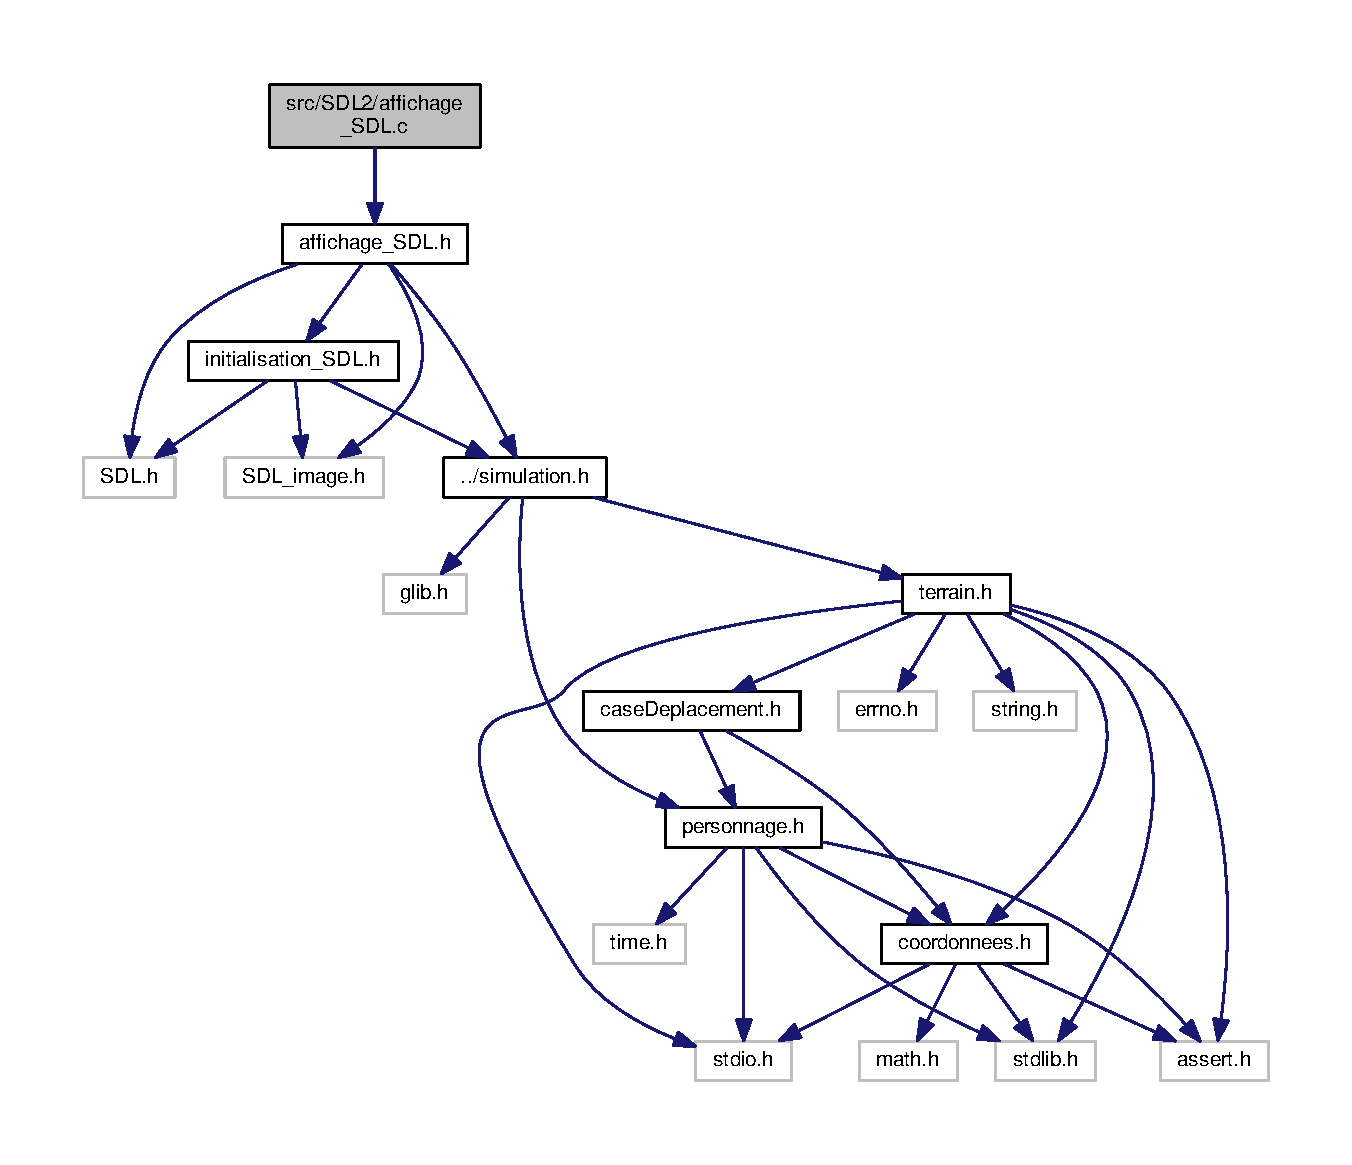
\includegraphics[width=350pt]{affichage__SDL_8c__incl}
\end{center}
\end{figure}
\subsection*{Fonctions}
\begin{DoxyCompactItemize}
\item 
void \hyperlink{affichage__SDL_8c_a278a2ffbb995f7837d4970a4d7435b63}{delay} (unsigned int frame\+Limit)
\item 
S\+D\+L\+\_\+\+Texture $\ast$ \hyperlink{affichage__SDL_8c_af3652d2a65ac26a4ec6170f48d9e12d8}{load\+Image} (char $\ast$name)
\item 
void \hyperlink{affichage__SDL_8c_a832a32567dcf778898e4bed9b109e612}{draw\+Image} (S\+D\+L\+\_\+\+Texture $\ast$image, int x, int y)
\begin{DoxyCompactList}\small\item\em Dessine la S\+D\+L\+\_\+\+Texture au coordonée XY. \end{DoxyCompactList}\item 
void \hyperlink{affichage__SDL_8c_a28eeadba58aaabe839e3467ce440a67c}{afficher\+Param\+Fenetre} (\hyperlink{simulation_8h_a1ab3bf4791ab776bb4bd460dcce3e8d7}{Simulation} $\ast$p\+Sim)
\begin{DoxyCompactList}\small\item\em Dessine les personnage de la simulation sur la fenetre. \end{DoxyCompactList}\item 
void \hyperlink{affichage__SDL_8c_a5c7272305c3e40540b846a7068612441}{affichage\+Fenetre} (\hyperlink{simulation_8h_a1ab3bf4791ab776bb4bd460dcce3e8d7}{Simulation} $\ast$p\+Sim)
\begin{DoxyCompactList}\small\item\em Dessine le terrain de la simulation sur la fenetre. \end{DoxyCompactList}\item 
void \hyperlink{affichage__SDL_8c_a06abdddfa81b0a2919a398fad146857b}{affichage\+Fenetre\+Editeur} (\hyperlink{terrain_8h_a11bbfdc6f8212f3246205cc0e7134136}{Terrain} $\ast$p\+Terrain)
\end{DoxyCompactItemize}


\subsection{Documentation des fonctions}
\index{affichage\+\_\+\+S\+D\+L.\+c@{affichage\+\_\+\+S\+D\+L.\+c}!affichage\+Fenetre@{affichage\+Fenetre}}
\index{affichage\+Fenetre@{affichage\+Fenetre}!affichage\+\_\+\+S\+D\+L.\+c@{affichage\+\_\+\+S\+D\+L.\+c}}
\subsubsection[{\texorpdfstring{affichage\+Fenetre(\+Simulation $\ast$p\+Sim)}{affichageFenetre(Simulation *pSim)}}]{\setlength{\rightskip}{0pt plus 5cm}void affichage\+Fenetre (
\begin{DoxyParamCaption}
\item[{{\bf Simulation} $\ast$}]{p\+Sim}
\end{DoxyParamCaption}
)}\hypertarget{affichage__SDL_8c_a5c7272305c3e40540b846a7068612441}{}\label{affichage__SDL_8c_a5c7272305c3e40540b846a7068612441}


Dessine le terrain de la simulation sur la fenetre. 


\begin{DoxyParams}{Paramètres}
{\em p\+Sim} & Pointeur vers la simulation à afficher \\
\hline
\end{DoxyParams}
\index{affichage\+\_\+\+S\+D\+L.\+c@{affichage\+\_\+\+S\+D\+L.\+c}!affichage\+Fenetre\+Editeur@{affichage\+Fenetre\+Editeur}}
\index{affichage\+Fenetre\+Editeur@{affichage\+Fenetre\+Editeur}!affichage\+\_\+\+S\+D\+L.\+c@{affichage\+\_\+\+S\+D\+L.\+c}}
\subsubsection[{\texorpdfstring{affichage\+Fenetre\+Editeur(\+Terrain $\ast$p\+Terrain)}{affichageFenetreEditeur(Terrain *pTerrain)}}]{\setlength{\rightskip}{0pt plus 5cm}void affichage\+Fenetre\+Editeur (
\begin{DoxyParamCaption}
\item[{{\bf Terrain} $\ast$}]{p\+Terrain}
\end{DoxyParamCaption}
)}\hypertarget{affichage__SDL_8c_a06abdddfa81b0a2919a398fad146857b}{}\label{affichage__SDL_8c_a06abdddfa81b0a2919a398fad146857b}
\index{affichage\+\_\+\+S\+D\+L.\+c@{affichage\+\_\+\+S\+D\+L.\+c}!afficher\+Param\+Fenetre@{afficher\+Param\+Fenetre}}
\index{afficher\+Param\+Fenetre@{afficher\+Param\+Fenetre}!affichage\+\_\+\+S\+D\+L.\+c@{affichage\+\_\+\+S\+D\+L.\+c}}
\subsubsection[{\texorpdfstring{afficher\+Param\+Fenetre(\+Simulation $\ast$p\+Sim)}{afficherParamFenetre(Simulation *pSim)}}]{\setlength{\rightskip}{0pt plus 5cm}void afficher\+Param\+Fenetre (
\begin{DoxyParamCaption}
\item[{{\bf Simulation} $\ast$}]{p\+Sim}
\end{DoxyParamCaption}
)}\hypertarget{affichage__SDL_8c_a28eeadba58aaabe839e3467ce440a67c}{}\label{affichage__SDL_8c_a28eeadba58aaabe839e3467ce440a67c}


Dessine les personnage de la simulation sur la fenetre. 


\begin{DoxyParams}{Paramètres}
{\em p\+Sim} & Pointeur vers la simulation à afficher \\
\hline
\end{DoxyParams}
\index{affichage\+\_\+\+S\+D\+L.\+c@{affichage\+\_\+\+S\+D\+L.\+c}!delay@{delay}}
\index{delay@{delay}!affichage\+\_\+\+S\+D\+L.\+c@{affichage\+\_\+\+S\+D\+L.\+c}}
\subsubsection[{\texorpdfstring{delay(unsigned int frame\+Limit)}{delay(unsigned int frameLimit)}}]{\setlength{\rightskip}{0pt plus 5cm}void delay (
\begin{DoxyParamCaption}
\item[{unsigned int}]{frame\+Limit}
\end{DoxyParamCaption}
)}\hypertarget{affichage__SDL_8c_a278a2ffbb995f7837d4970a4d7435b63}{}\label{affichage__SDL_8c_a278a2ffbb995f7837d4970a4d7435b63}
\index{affichage\+\_\+\+S\+D\+L.\+c@{affichage\+\_\+\+S\+D\+L.\+c}!draw\+Image@{draw\+Image}}
\index{draw\+Image@{draw\+Image}!affichage\+\_\+\+S\+D\+L.\+c@{affichage\+\_\+\+S\+D\+L.\+c}}
\subsubsection[{\texorpdfstring{draw\+Image(\+S\+D\+L\+\_\+\+Texture $\ast$image, int x, int y)}{drawImage(SDL_Texture *image, int x, int y)}}]{\setlength{\rightskip}{0pt plus 5cm}void draw\+Image (
\begin{DoxyParamCaption}
\item[{S\+D\+L\+\_\+\+Texture $\ast$}]{image, }
\item[{int}]{x, }
\item[{int}]{y}
\end{DoxyParamCaption}
)}\hypertarget{affichage__SDL_8c_a832a32567dcf778898e4bed9b109e612}{}\label{affichage__SDL_8c_a832a32567dcf778898e4bed9b109e612}


Dessine la S\+D\+L\+\_\+\+Texture au coordonée XY. 


\begin{DoxyParams}{Paramètres}
{\em image} & Pointeur vers la S\+D\+L\+\_\+texture a dessiner \\
\hline
{\em x} & Coordonnées en X ou dessiner \\
\hline
{\em y} & Coordonnées en Y ou dessiner \\
\hline
\end{DoxyParams}
\index{affichage\+\_\+\+S\+D\+L.\+c@{affichage\+\_\+\+S\+D\+L.\+c}!load\+Image@{load\+Image}}
\index{load\+Image@{load\+Image}!affichage\+\_\+\+S\+D\+L.\+c@{affichage\+\_\+\+S\+D\+L.\+c}}
\subsubsection[{\texorpdfstring{load\+Image(char $\ast$name)}{loadImage(char *name)}}]{\setlength{\rightskip}{0pt plus 5cm}S\+D\+L\+\_\+\+Texture$\ast$ load\+Image (
\begin{DoxyParamCaption}
\item[{char $\ast$}]{name}
\end{DoxyParamCaption}
)}\hypertarget{affichage__SDL_8c_af3652d2a65ac26a4ec6170f48d9e12d8}{}\label{affichage__SDL_8c_af3652d2a65ac26a4ec6170f48d9e12d8}

\hypertarget{affichage__SDL_8h}{}\section{Référence du fichier src/\+S\+D\+L2/affichage\+\_\+\+S\+DL.h}
\label{affichage__SDL_8h}\index{src/\+S\+D\+L2/affichage\+\_\+\+S\+D\+L.\+h@{src/\+S\+D\+L2/affichage\+\_\+\+S\+D\+L.\+h}}


Définit les fonctions d\textquotesingle{}affichage S\+DL.  


{\ttfamily \#include $<$S\+D\+L.\+h$>$}\\*
{\ttfamily \#include $<$S\+D\+L\+\_\+image.\+h$>$}\\*
{\ttfamily \#include \char`\"{}../simulation.\+h\char`\"{}}\\*
{\ttfamily \#include \char`\"{}initialisation\+\_\+\+S\+D\+L.\+h\char`\"{}}\\*
Graphe des dépendances par inclusion de affichage\+\_\+\+S\+D\+L.\+h\+:
\nopagebreak
\begin{figure}[H]
\begin{center}
\leavevmode
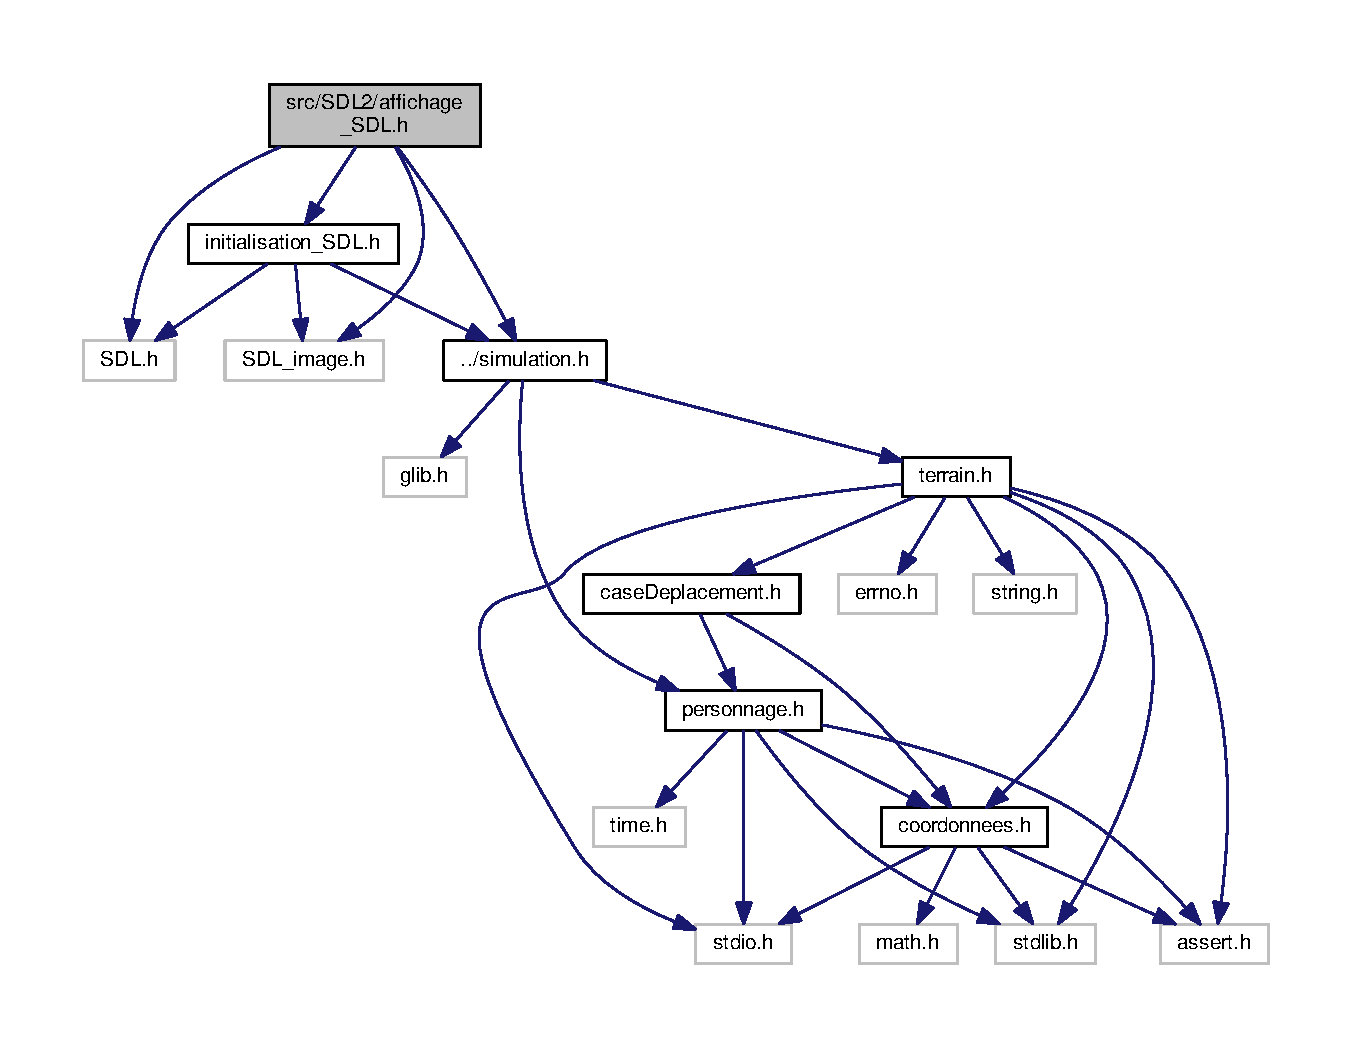
\includegraphics[width=350pt]{affichage__SDL_8h__incl}
\end{center}
\end{figure}
Ce graphe montre quels fichiers incluent directement ou indirectement ce fichier \+:
\nopagebreak
\begin{figure}[H]
\begin{center}
\leavevmode
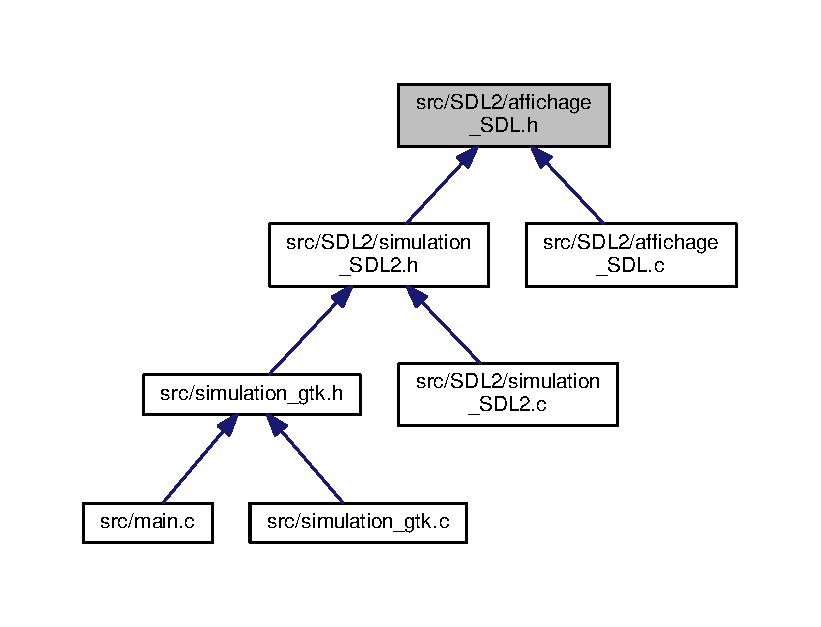
\includegraphics[width=350pt]{affichage__SDL_8h__dep__incl}
\end{center}
\end{figure}
\subsection*{Fonctions}
\begin{DoxyCompactItemize}
\item 
void \hyperlink{affichage__SDL_8h_a278a2ffbb995f7837d4970a4d7435b63}{delay} (unsigned int frame\+Limit)
\item 
S\+D\+L\+\_\+\+Texture $\ast$ \hyperlink{affichage__SDL_8h_af3652d2a65ac26a4ec6170f48d9e12d8}{load\+Image} (char $\ast$name)
\item 
void \hyperlink{affichage__SDL_8h_a832a32567dcf778898e4bed9b109e612}{draw\+Image} (S\+D\+L\+\_\+\+Texture $\ast$image, int x, int y)
\begin{DoxyCompactList}\small\item\em Dessine la S\+D\+L\+\_\+\+Texture au coordonée XY. \end{DoxyCompactList}\item 
void \hyperlink{affichage__SDL_8h_a28eeadba58aaabe839e3467ce440a67c}{afficher\+Param\+Fenetre} (\hyperlink{simulation_8h_a1ab3bf4791ab776bb4bd460dcce3e8d7}{Simulation} $\ast$p\+Sim)
\begin{DoxyCompactList}\small\item\em Dessine les personnage de la simulation sur la fenetre. \end{DoxyCompactList}\item 
void \hyperlink{affichage__SDL_8h_a5c7272305c3e40540b846a7068612441}{affichage\+Fenetre} (\hyperlink{simulation_8h_a1ab3bf4791ab776bb4bd460dcce3e8d7}{Simulation} $\ast$p\+Sim)
\begin{DoxyCompactList}\small\item\em Dessine le terrain de la simulation sur la fenetre. \end{DoxyCompactList}\item 
void \hyperlink{affichage__SDL_8h_aefd5d93398affc282898e4e087e37eee}{affichage\+Fenetre\+Editeur} ()
\begin{DoxyCompactList}\small\item\em Dessine le terrain vierge pour l\textquotesingle{}editeur sur la fenetre. \end{DoxyCompactList}\end{DoxyCompactItemize}


\subsection{Description détaillée}
Définit les fonctions d\textquotesingle{}affichage S\+DL. 



\subsection{Documentation des fonctions}
\index{affichage\+\_\+\+S\+D\+L.\+h@{affichage\+\_\+\+S\+D\+L.\+h}!affichage\+Fenetre@{affichage\+Fenetre}}
\index{affichage\+Fenetre@{affichage\+Fenetre}!affichage\+\_\+\+S\+D\+L.\+h@{affichage\+\_\+\+S\+D\+L.\+h}}
\subsubsection[{\texorpdfstring{affichage\+Fenetre(\+Simulation $\ast$p\+Sim)}{affichageFenetre(Simulation *pSim)}}]{\setlength{\rightskip}{0pt plus 5cm}void affichage\+Fenetre (
\begin{DoxyParamCaption}
\item[{{\bf Simulation} $\ast$}]{p\+Sim}
\end{DoxyParamCaption}
)}\hypertarget{affichage__SDL_8h_a5c7272305c3e40540b846a7068612441}{}\label{affichage__SDL_8h_a5c7272305c3e40540b846a7068612441}


Dessine le terrain de la simulation sur la fenetre. 


\begin{DoxyParams}{Paramètres}
{\em p\+Sim} & Pointeur vers la simulation à afficher \\
\hline
\end{DoxyParams}
\index{affichage\+\_\+\+S\+D\+L.\+h@{affichage\+\_\+\+S\+D\+L.\+h}!affichage\+Fenetre\+Editeur@{affichage\+Fenetre\+Editeur}}
\index{affichage\+Fenetre\+Editeur@{affichage\+Fenetre\+Editeur}!affichage\+\_\+\+S\+D\+L.\+h@{affichage\+\_\+\+S\+D\+L.\+h}}
\subsubsection[{\texorpdfstring{affichage\+Fenetre\+Editeur()}{affichageFenetreEditeur()}}]{\setlength{\rightskip}{0pt plus 5cm}void affichage\+Fenetre\+Editeur (
\begin{DoxyParamCaption}
{}
\end{DoxyParamCaption}
)}\hypertarget{affichage__SDL_8h_aefd5d93398affc282898e4e087e37eee}{}\label{affichage__SDL_8h_aefd5d93398affc282898e4e087e37eee}


Dessine le terrain vierge pour l\textquotesingle{}editeur sur la fenetre. 

\index{affichage\+\_\+\+S\+D\+L.\+h@{affichage\+\_\+\+S\+D\+L.\+h}!afficher\+Param\+Fenetre@{afficher\+Param\+Fenetre}}
\index{afficher\+Param\+Fenetre@{afficher\+Param\+Fenetre}!affichage\+\_\+\+S\+D\+L.\+h@{affichage\+\_\+\+S\+D\+L.\+h}}
\subsubsection[{\texorpdfstring{afficher\+Param\+Fenetre(\+Simulation $\ast$p\+Sim)}{afficherParamFenetre(Simulation *pSim)}}]{\setlength{\rightskip}{0pt plus 5cm}void afficher\+Param\+Fenetre (
\begin{DoxyParamCaption}
\item[{{\bf Simulation} $\ast$}]{p\+Sim}
\end{DoxyParamCaption}
)}\hypertarget{affichage__SDL_8h_a28eeadba58aaabe839e3467ce440a67c}{}\label{affichage__SDL_8h_a28eeadba58aaabe839e3467ce440a67c}


Dessine les personnage de la simulation sur la fenetre. 


\begin{DoxyParams}{Paramètres}
{\em p\+Sim} & Pointeur vers la simulation à afficher \\
\hline
\end{DoxyParams}
\index{affichage\+\_\+\+S\+D\+L.\+h@{affichage\+\_\+\+S\+D\+L.\+h}!delay@{delay}}
\index{delay@{delay}!affichage\+\_\+\+S\+D\+L.\+h@{affichage\+\_\+\+S\+D\+L.\+h}}
\subsubsection[{\texorpdfstring{delay(unsigned int frame\+Limit)}{delay(unsigned int frameLimit)}}]{\setlength{\rightskip}{0pt plus 5cm}void delay (
\begin{DoxyParamCaption}
\item[{unsigned int}]{frame\+Limit}
\end{DoxyParamCaption}
)}\hypertarget{affichage__SDL_8h_a278a2ffbb995f7837d4970a4d7435b63}{}\label{affichage__SDL_8h_a278a2ffbb995f7837d4970a4d7435b63}
\index{affichage\+\_\+\+S\+D\+L.\+h@{affichage\+\_\+\+S\+D\+L.\+h}!draw\+Image@{draw\+Image}}
\index{draw\+Image@{draw\+Image}!affichage\+\_\+\+S\+D\+L.\+h@{affichage\+\_\+\+S\+D\+L.\+h}}
\subsubsection[{\texorpdfstring{draw\+Image(\+S\+D\+L\+\_\+\+Texture $\ast$image, int x, int y)}{drawImage(SDL_Texture *image, int x, int y)}}]{\setlength{\rightskip}{0pt plus 5cm}void draw\+Image (
\begin{DoxyParamCaption}
\item[{S\+D\+L\+\_\+\+Texture $\ast$}]{image, }
\item[{int}]{x, }
\item[{int}]{y}
\end{DoxyParamCaption}
)}\hypertarget{affichage__SDL_8h_a832a32567dcf778898e4bed9b109e612}{}\label{affichage__SDL_8h_a832a32567dcf778898e4bed9b109e612}


Dessine la S\+D\+L\+\_\+\+Texture au coordonée XY. 


\begin{DoxyParams}{Paramètres}
{\em image} & Pointeur vers la S\+D\+L\+\_\+texture a dessiner \\
\hline
{\em x} & Coordonnées en X ou dessiner \\
\hline
{\em y} & Coordonnées en Y ou dessiner \\
\hline
\end{DoxyParams}
\index{affichage\+\_\+\+S\+D\+L.\+h@{affichage\+\_\+\+S\+D\+L.\+h}!load\+Image@{load\+Image}}
\index{load\+Image@{load\+Image}!affichage\+\_\+\+S\+D\+L.\+h@{affichage\+\_\+\+S\+D\+L.\+h}}
\subsubsection[{\texorpdfstring{load\+Image(char $\ast$name)}{loadImage(char *name)}}]{\setlength{\rightskip}{0pt plus 5cm}S\+D\+L\+\_\+\+Texture$\ast$ load\+Image (
\begin{DoxyParamCaption}
\item[{char $\ast$}]{name}
\end{DoxyParamCaption}
)}\hypertarget{affichage__SDL_8h_af3652d2a65ac26a4ec6170f48d9e12d8}{}\label{affichage__SDL_8h_af3652d2a65ac26a4ec6170f48d9e12d8}

\hypertarget{initialisation__SDL_8c}{}\section{Référence du fichier src/\+S\+D\+L2/initialisation\+\_\+\+S\+DL.c}
\label{initialisation__SDL_8c}\index{src/\+S\+D\+L2/initialisation\+\_\+\+S\+D\+L.\+c@{src/\+S\+D\+L2/initialisation\+\_\+\+S\+D\+L.\+c}}
{\ttfamily \#include \char`\"{}initialisation\+\_\+\+S\+D\+L.\+h\char`\"{}}\\*
Graphe des dépendances par inclusion de initialisation\+\_\+\+S\+D\+L.\+c\+:
\nopagebreak
\begin{figure}[H]
\begin{center}
\leavevmode
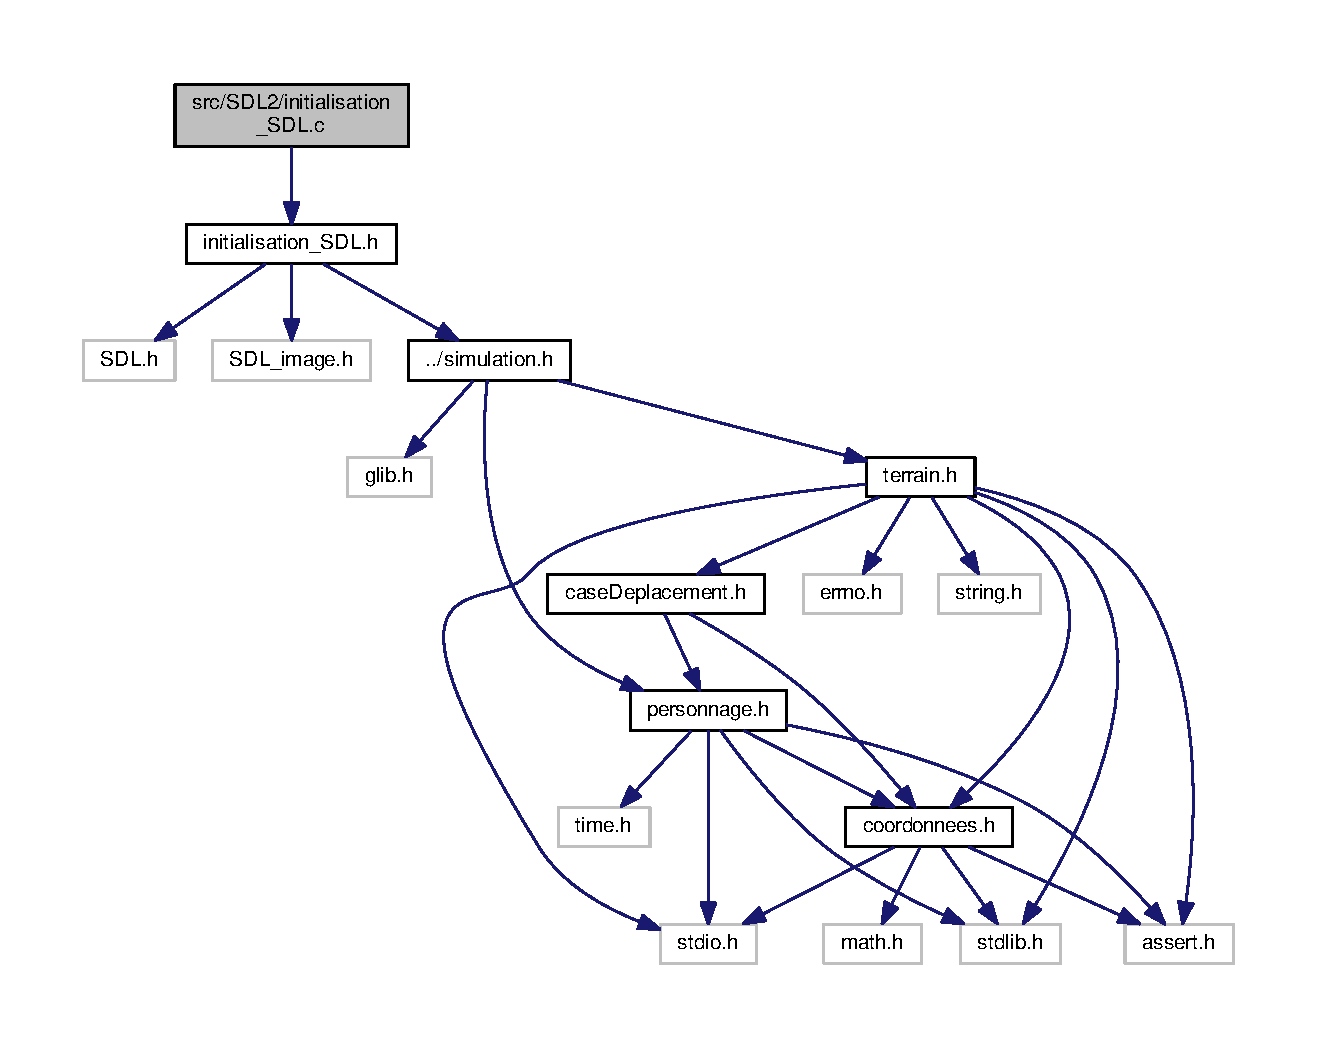
\includegraphics[width=350pt]{initialisation__SDL_8c__incl}
\end{center}
\end{figure}
\subsection*{Fonctions}
\begin{DoxyCompactItemize}
\item 
S\+D\+L\+\_\+\+Renderer $\ast$ \hyperlink{initialisation__SDL_8c_af99f62e774acad50e71f3cd462e80b60}{getrenderer} ()
\begin{DoxyCompactList}\small\item\em Recupère le renderer actuellement utilisé \end{DoxyCompactList}\item 
void \hyperlink{initialisation__SDL_8c_acce1a8c22dcc885898abedabfcd63ac9}{init} (char $\ast$title, \hyperlink{simulation_8h_a1ab3bf4791ab776bb4bd460dcce3e8d7}{Simulation} $\ast$p\+Sim)
\begin{DoxyCompactList}\small\item\em Initilialise une fenetre avec le nom donné et les dimension définie dans le define pour la fenetre de simulation. \end{DoxyCompactList}\item 
void \hyperlink{initialisation__SDL_8c_a3b0c2b5ffb97c7f0aa294d96306ef3f5}{init\+Editeur} (char $\ast$title, \hyperlink{terrain_8h_a11bbfdc6f8212f3246205cc0e7134136}{Terrain} $\ast$p\+Terrain)
\begin{DoxyCompactList}\small\item\em Initilialise une fenetre avec le nom donné et les dimension définie dans le define pour la fenetre de l\textquotesingle{}editeur. \end{DoxyCompactList}\item 
void \hyperlink{initialisation__SDL_8c_a4b66d5e31b5dc18b314c8a68163263bd}{cleanup} ()
\begin{DoxyCompactList}\small\item\em Detruit la fenetre, le rendu et ferme S\+DL. \end{DoxyCompactList}\end{DoxyCompactItemize}
\subsection*{Variables}
\begin{DoxyCompactItemize}
\item 
S\+D\+L\+\_\+\+Window $\ast$ \hyperlink{initialisation__SDL_8c_ae04e09e4e3831bfc1632c509ae37dcec}{screen}
\item 
S\+D\+L\+\_\+\+Renderer $\ast$ \hyperlink{initialisation__SDL_8c_a966da7a60c4ea3ba301e26ccc5efe452}{renderer}
\end{DoxyCompactItemize}


\subsection{Documentation des fonctions}
\index{initialisation\+\_\+\+S\+D\+L.\+c@{initialisation\+\_\+\+S\+D\+L.\+c}!cleanup@{cleanup}}
\index{cleanup@{cleanup}!initialisation\+\_\+\+S\+D\+L.\+c@{initialisation\+\_\+\+S\+D\+L.\+c}}
\subsubsection[{\texorpdfstring{cleanup()}{cleanup()}}]{\setlength{\rightskip}{0pt plus 5cm}void cleanup (
\begin{DoxyParamCaption}
{}
\end{DoxyParamCaption}
)}\hypertarget{initialisation__SDL_8c_a4b66d5e31b5dc18b314c8a68163263bd}{}\label{initialisation__SDL_8c_a4b66d5e31b5dc18b314c8a68163263bd}


Detruit la fenetre, le rendu et ferme S\+DL. 

\index{initialisation\+\_\+\+S\+D\+L.\+c@{initialisation\+\_\+\+S\+D\+L.\+c}!getrenderer@{getrenderer}}
\index{getrenderer@{getrenderer}!initialisation\+\_\+\+S\+D\+L.\+c@{initialisation\+\_\+\+S\+D\+L.\+c}}
\subsubsection[{\texorpdfstring{getrenderer()}{getrenderer()}}]{\setlength{\rightskip}{0pt plus 5cm}S\+D\+L\+\_\+\+Renderer$\ast$ getrenderer (
\begin{DoxyParamCaption}
{}
\end{DoxyParamCaption}
)}\hypertarget{initialisation__SDL_8c_af99f62e774acad50e71f3cd462e80b60}{}\label{initialisation__SDL_8c_af99f62e774acad50e71f3cd462e80b60}


Recupère le renderer actuellement utilisé 

\begin{DoxyReturn}{Renvoie}
Pointeur vers le S\+D\+L\+\_\+\+Renderer utilisé 
\end{DoxyReturn}
\index{initialisation\+\_\+\+S\+D\+L.\+c@{initialisation\+\_\+\+S\+D\+L.\+c}!init@{init}}
\index{init@{init}!initialisation\+\_\+\+S\+D\+L.\+c@{initialisation\+\_\+\+S\+D\+L.\+c}}
\subsubsection[{\texorpdfstring{init(char $\ast$title, Simulation $\ast$p\+Sim)}{init(char *title, Simulation *pSim)}}]{\setlength{\rightskip}{0pt plus 5cm}void init (
\begin{DoxyParamCaption}
\item[{char $\ast$}]{title, }
\item[{{\bf Simulation} $\ast$}]{p\+Sim}
\end{DoxyParamCaption}
)}\hypertarget{initialisation__SDL_8c_acce1a8c22dcc885898abedabfcd63ac9}{}\label{initialisation__SDL_8c_acce1a8c22dcc885898abedabfcd63ac9}


Initilialise une fenetre avec le nom donné et les dimension définie dans le define pour la fenetre de simulation. 


\begin{DoxyParams}{Paramètres}
{\em title} & Chaine de caractères du nom de la fenetre a initiliser \\
\hline
{\em p\+Sim} & Pointeur vers la simulation \\
\hline
\end{DoxyParams}
\index{initialisation\+\_\+\+S\+D\+L.\+c@{initialisation\+\_\+\+S\+D\+L.\+c}!init\+Editeur@{init\+Editeur}}
\index{init\+Editeur@{init\+Editeur}!initialisation\+\_\+\+S\+D\+L.\+c@{initialisation\+\_\+\+S\+D\+L.\+c}}
\subsubsection[{\texorpdfstring{init\+Editeur(char $\ast$title, Terrain $\ast$p\+Terrain)}{initEditeur(char *title, Terrain *pTerrain)}}]{\setlength{\rightskip}{0pt plus 5cm}void init\+Editeur (
\begin{DoxyParamCaption}
\item[{char $\ast$}]{title, }
\item[{{\bf Terrain} $\ast$}]{p\+Terrain}
\end{DoxyParamCaption}
)}\hypertarget{initialisation__SDL_8c_a3b0c2b5ffb97c7f0aa294d96306ef3f5}{}\label{initialisation__SDL_8c_a3b0c2b5ffb97c7f0aa294d96306ef3f5}


Initilialise une fenetre avec le nom donné et les dimension définie dans le define pour la fenetre de l\textquotesingle{}editeur. 


\begin{DoxyParams}{Paramètres}
{\em title} & Chaine de caractères du nom de la fenetre a initiliser \\
\hline
{\em p\+Terrain} & Pointeur vers le terrain à afficher \\
\hline
\end{DoxyParams}


\subsection{Documentation des variables}
\index{initialisation\+\_\+\+S\+D\+L.\+c@{initialisation\+\_\+\+S\+D\+L.\+c}!renderer@{renderer}}
\index{renderer@{renderer}!initialisation\+\_\+\+S\+D\+L.\+c@{initialisation\+\_\+\+S\+D\+L.\+c}}
\subsubsection[{\texorpdfstring{renderer}{renderer}}]{\setlength{\rightskip}{0pt plus 5cm}S\+D\+L\+\_\+\+Renderer$\ast$ renderer}\hypertarget{initialisation__SDL_8c_a966da7a60c4ea3ba301e26ccc5efe452}{}\label{initialisation__SDL_8c_a966da7a60c4ea3ba301e26ccc5efe452}
\index{initialisation\+\_\+\+S\+D\+L.\+c@{initialisation\+\_\+\+S\+D\+L.\+c}!screen@{screen}}
\index{screen@{screen}!initialisation\+\_\+\+S\+D\+L.\+c@{initialisation\+\_\+\+S\+D\+L.\+c}}
\subsubsection[{\texorpdfstring{screen}{screen}}]{\setlength{\rightskip}{0pt plus 5cm}S\+D\+L\+\_\+\+Window$\ast$ screen}\hypertarget{initialisation__SDL_8c_ae04e09e4e3831bfc1632c509ae37dcec}{}\label{initialisation__SDL_8c_ae04e09e4e3831bfc1632c509ae37dcec}

\hypertarget{initialisation__SDL_8h}{}\section{Référence du fichier src/\+S\+D\+L2/initialisation\+\_\+\+S\+DL.h}
\label{initialisation__SDL_8h}\index{src/\+S\+D\+L2/initialisation\+\_\+\+S\+D\+L.\+h@{src/\+S\+D\+L2/initialisation\+\_\+\+S\+D\+L.\+h}}


Définit les fonction pour l\textquotesingle{}initialisation de S\+DL.  


{\ttfamily \#include $<$S\+D\+L.\+h$>$}\\*
{\ttfamily \#include $<$S\+D\+L\+\_\+image.\+h$>$}\\*
{\ttfamily \#include \char`\"{}../simulation.\+h\char`\"{}}\\*
Graphe des dépendances par inclusion de initialisation\+\_\+\+S\+D\+L.\+h\+:
\nopagebreak
\begin{figure}[H]
\begin{center}
\leavevmode
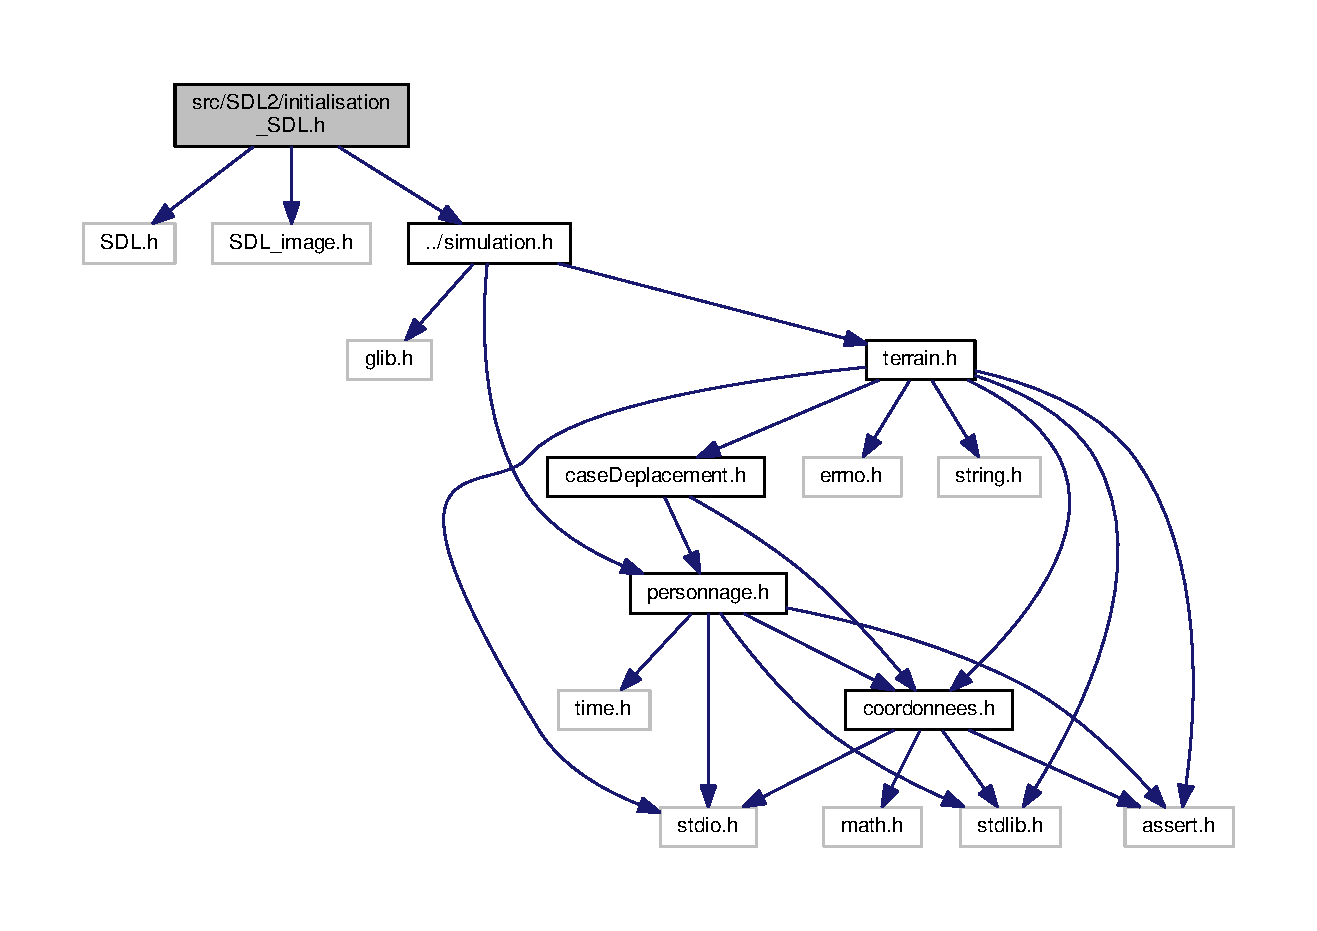
\includegraphics[width=350pt]{initialisation__SDL_8h__incl}
\end{center}
\end{figure}
Ce graphe montre quels fichiers incluent directement ou indirectement ce fichier \+:
\nopagebreak
\begin{figure}[H]
\begin{center}
\leavevmode
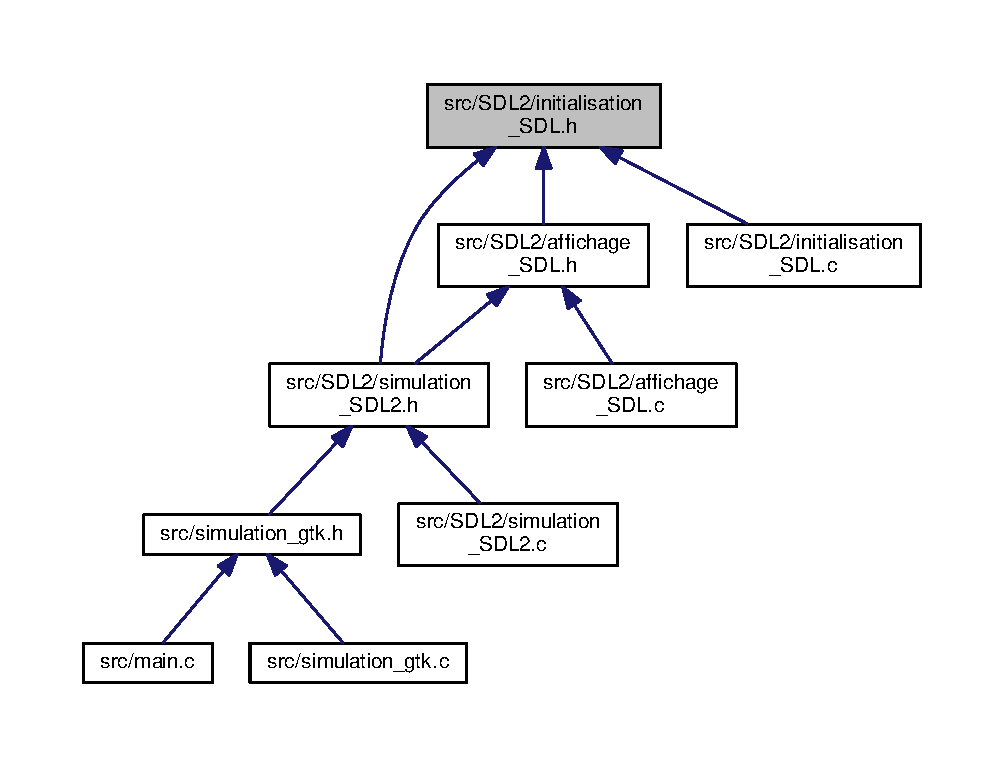
\includegraphics[width=350pt]{initialisation__SDL_8h__dep__incl}
\end{center}
\end{figure}
\subsection*{Macros}
\begin{DoxyCompactItemize}
\item 
\#define \hyperlink{initialisation__SDL_8h_ae4a8f36daa8d89cf5e2cddb77b7ce93a}{R\+E\+N\+D\+E\+R\+E\+R\+S\+C\+A\+LE}~0.\+3
\item 
\#define \hyperlink{initialisation__SDL_8h_ac256520bdfa378b81535036531b70079}{D\+E\+L\+A\+Y\+R\+E\+F\+R\+E\+SH}~300
\end{DoxyCompactItemize}
\subsection*{Fonctions}
\begin{DoxyCompactItemize}
\item 
S\+D\+L\+\_\+\+Renderer $\ast$ \hyperlink{initialisation__SDL_8h_af99f62e774acad50e71f3cd462e80b60}{getrenderer} ()
\begin{DoxyCompactList}\small\item\em Recupère le renderer actuellement utilisé \end{DoxyCompactList}\item 
void \hyperlink{initialisation__SDL_8h_acce1a8c22dcc885898abedabfcd63ac9}{init} (char $\ast$title, \hyperlink{simulation_8h_a1ab3bf4791ab776bb4bd460dcce3e8d7}{Simulation} $\ast$p\+Sim)
\begin{DoxyCompactList}\small\item\em Initilialise une fenetre avec le nom donné et les dimension définie dans le define pour la fenetre de simulation. \end{DoxyCompactList}\item 
void \hyperlink{initialisation__SDL_8h_a3b0c2b5ffb97c7f0aa294d96306ef3f5}{init\+Editeur} (char $\ast$title, \hyperlink{terrain_8h_a11bbfdc6f8212f3246205cc0e7134136}{Terrain} $\ast$p\+Terrain)
\begin{DoxyCompactList}\small\item\em Initilialise une fenetre avec le nom donné et les dimension définie dans le define pour la fenetre de l\textquotesingle{}editeur. \end{DoxyCompactList}\item 
void \hyperlink{initialisation__SDL_8h_a4b66d5e31b5dc18b314c8a68163263bd}{cleanup} ()
\begin{DoxyCompactList}\small\item\em Detruit la fenetre, le rendu et ferme S\+DL. \end{DoxyCompactList}\end{DoxyCompactItemize}


\subsection{Description détaillée}
Définit les fonction pour l\textquotesingle{}initialisation de S\+DL. 



\subsection{Documentation des macros}
\index{initialisation\+\_\+\+S\+D\+L.\+h@{initialisation\+\_\+\+S\+D\+L.\+h}!D\+E\+L\+A\+Y\+R\+E\+F\+R\+E\+SH@{D\+E\+L\+A\+Y\+R\+E\+F\+R\+E\+SH}}
\index{D\+E\+L\+A\+Y\+R\+E\+F\+R\+E\+SH@{D\+E\+L\+A\+Y\+R\+E\+F\+R\+E\+SH}!initialisation\+\_\+\+S\+D\+L.\+h@{initialisation\+\_\+\+S\+D\+L.\+h}}
\subsubsection[{\texorpdfstring{D\+E\+L\+A\+Y\+R\+E\+F\+R\+E\+SH}{DELAYREFRESH}}]{\setlength{\rightskip}{0pt plus 5cm}\#define D\+E\+L\+A\+Y\+R\+E\+F\+R\+E\+SH~300}\hypertarget{initialisation__SDL_8h_ac256520bdfa378b81535036531b70079}{}\label{initialisation__SDL_8h_ac256520bdfa378b81535036531b70079}
\index{initialisation\+\_\+\+S\+D\+L.\+h@{initialisation\+\_\+\+S\+D\+L.\+h}!R\+E\+N\+D\+E\+R\+E\+R\+S\+C\+A\+LE@{R\+E\+N\+D\+E\+R\+E\+R\+S\+C\+A\+LE}}
\index{R\+E\+N\+D\+E\+R\+E\+R\+S\+C\+A\+LE@{R\+E\+N\+D\+E\+R\+E\+R\+S\+C\+A\+LE}!initialisation\+\_\+\+S\+D\+L.\+h@{initialisation\+\_\+\+S\+D\+L.\+h}}
\subsubsection[{\texorpdfstring{R\+E\+N\+D\+E\+R\+E\+R\+S\+C\+A\+LE}{RENDERERSCALE}}]{\setlength{\rightskip}{0pt plus 5cm}\#define R\+E\+N\+D\+E\+R\+E\+R\+S\+C\+A\+LE~0.\+3}\hypertarget{initialisation__SDL_8h_ae4a8f36daa8d89cf5e2cddb77b7ce93a}{}\label{initialisation__SDL_8h_ae4a8f36daa8d89cf5e2cddb77b7ce93a}


\subsection{Documentation des fonctions}
\index{initialisation\+\_\+\+S\+D\+L.\+h@{initialisation\+\_\+\+S\+D\+L.\+h}!cleanup@{cleanup}}
\index{cleanup@{cleanup}!initialisation\+\_\+\+S\+D\+L.\+h@{initialisation\+\_\+\+S\+D\+L.\+h}}
\subsubsection[{\texorpdfstring{cleanup()}{cleanup()}}]{\setlength{\rightskip}{0pt plus 5cm}void cleanup (
\begin{DoxyParamCaption}
{}
\end{DoxyParamCaption}
)}\hypertarget{initialisation__SDL_8h_a4b66d5e31b5dc18b314c8a68163263bd}{}\label{initialisation__SDL_8h_a4b66d5e31b5dc18b314c8a68163263bd}


Detruit la fenetre, le rendu et ferme S\+DL. 

\index{initialisation\+\_\+\+S\+D\+L.\+h@{initialisation\+\_\+\+S\+D\+L.\+h}!getrenderer@{getrenderer}}
\index{getrenderer@{getrenderer}!initialisation\+\_\+\+S\+D\+L.\+h@{initialisation\+\_\+\+S\+D\+L.\+h}}
\subsubsection[{\texorpdfstring{getrenderer()}{getrenderer()}}]{\setlength{\rightskip}{0pt plus 5cm}S\+D\+L\+\_\+\+Renderer$\ast$ getrenderer (
\begin{DoxyParamCaption}
{}
\end{DoxyParamCaption}
)}\hypertarget{initialisation__SDL_8h_af99f62e774acad50e71f3cd462e80b60}{}\label{initialisation__SDL_8h_af99f62e774acad50e71f3cd462e80b60}


Recupère le renderer actuellement utilisé 

\begin{DoxyReturn}{Renvoie}
Pointeur vers le S\+D\+L\+\_\+\+Renderer utilisé 
\end{DoxyReturn}
\index{initialisation\+\_\+\+S\+D\+L.\+h@{initialisation\+\_\+\+S\+D\+L.\+h}!init@{init}}
\index{init@{init}!initialisation\+\_\+\+S\+D\+L.\+h@{initialisation\+\_\+\+S\+D\+L.\+h}}
\subsubsection[{\texorpdfstring{init(char $\ast$title, Simulation $\ast$p\+Sim)}{init(char *title, Simulation *pSim)}}]{\setlength{\rightskip}{0pt plus 5cm}void init (
\begin{DoxyParamCaption}
\item[{char $\ast$}]{title, }
\item[{{\bf Simulation} $\ast$}]{p\+Sim}
\end{DoxyParamCaption}
)}\hypertarget{initialisation__SDL_8h_acce1a8c22dcc885898abedabfcd63ac9}{}\label{initialisation__SDL_8h_acce1a8c22dcc885898abedabfcd63ac9}


Initilialise une fenetre avec le nom donné et les dimension définie dans le define pour la fenetre de simulation. 


\begin{DoxyParams}{Paramètres}
{\em title} & Chaine de caractères du nom de la fenetre a initiliser \\
\hline
{\em p\+Sim} & Pointeur vers la simulation \\
\hline
\end{DoxyParams}
\index{initialisation\+\_\+\+S\+D\+L.\+h@{initialisation\+\_\+\+S\+D\+L.\+h}!init\+Editeur@{init\+Editeur}}
\index{init\+Editeur@{init\+Editeur}!initialisation\+\_\+\+S\+D\+L.\+h@{initialisation\+\_\+\+S\+D\+L.\+h}}
\subsubsection[{\texorpdfstring{init\+Editeur(char $\ast$title, Terrain $\ast$p\+Terrain)}{initEditeur(char *title, Terrain *pTerrain)}}]{\setlength{\rightskip}{0pt plus 5cm}void init\+Editeur (
\begin{DoxyParamCaption}
\item[{char $\ast$}]{title, }
\item[{{\bf Terrain} $\ast$}]{p\+Terrain}
\end{DoxyParamCaption}
)}\hypertarget{initialisation__SDL_8h_a3b0c2b5ffb97c7f0aa294d96306ef3f5}{}\label{initialisation__SDL_8h_a3b0c2b5ffb97c7f0aa294d96306ef3f5}


Initilialise une fenetre avec le nom donné et les dimension définie dans le define pour la fenetre de l\textquotesingle{}editeur. 


\begin{DoxyParams}{Paramètres}
{\em title} & Chaine de caractères du nom de la fenetre a initiliser \\
\hline
{\em p\+Terrain} & Pointeur vers le terrain à afficher \\
\hline
\end{DoxyParams}

\hypertarget{simulation__SDL2_8c}{}\section{Référence du fichier src/\+S\+D\+L2/simulation\+\_\+\+S\+D\+L2.c}
\label{simulation__SDL2_8c}\index{src/\+S\+D\+L2/simulation\+\_\+\+S\+D\+L2.\+c@{src/\+S\+D\+L2/simulation\+\_\+\+S\+D\+L2.\+c}}
{\ttfamily \#include $<$S\+D\+L2/\+S\+D\+L.\+h$>$}\\*
{\ttfamily \#include $<$S\+D\+L2/\+S\+D\+L\+\_\+image.\+h$>$}\\*
{\ttfamily \#include \char`\"{}simulation\+\_\+\+S\+D\+L2.\+h\char`\"{}}\\*
{\ttfamily \#include \char`\"{}../simulation.\+h\char`\"{}}\\*
Graphe des dépendances par inclusion de simulation\+\_\+\+S\+D\+L2.\+c\+:
\nopagebreak
\begin{figure}[H]
\begin{center}
\leavevmode
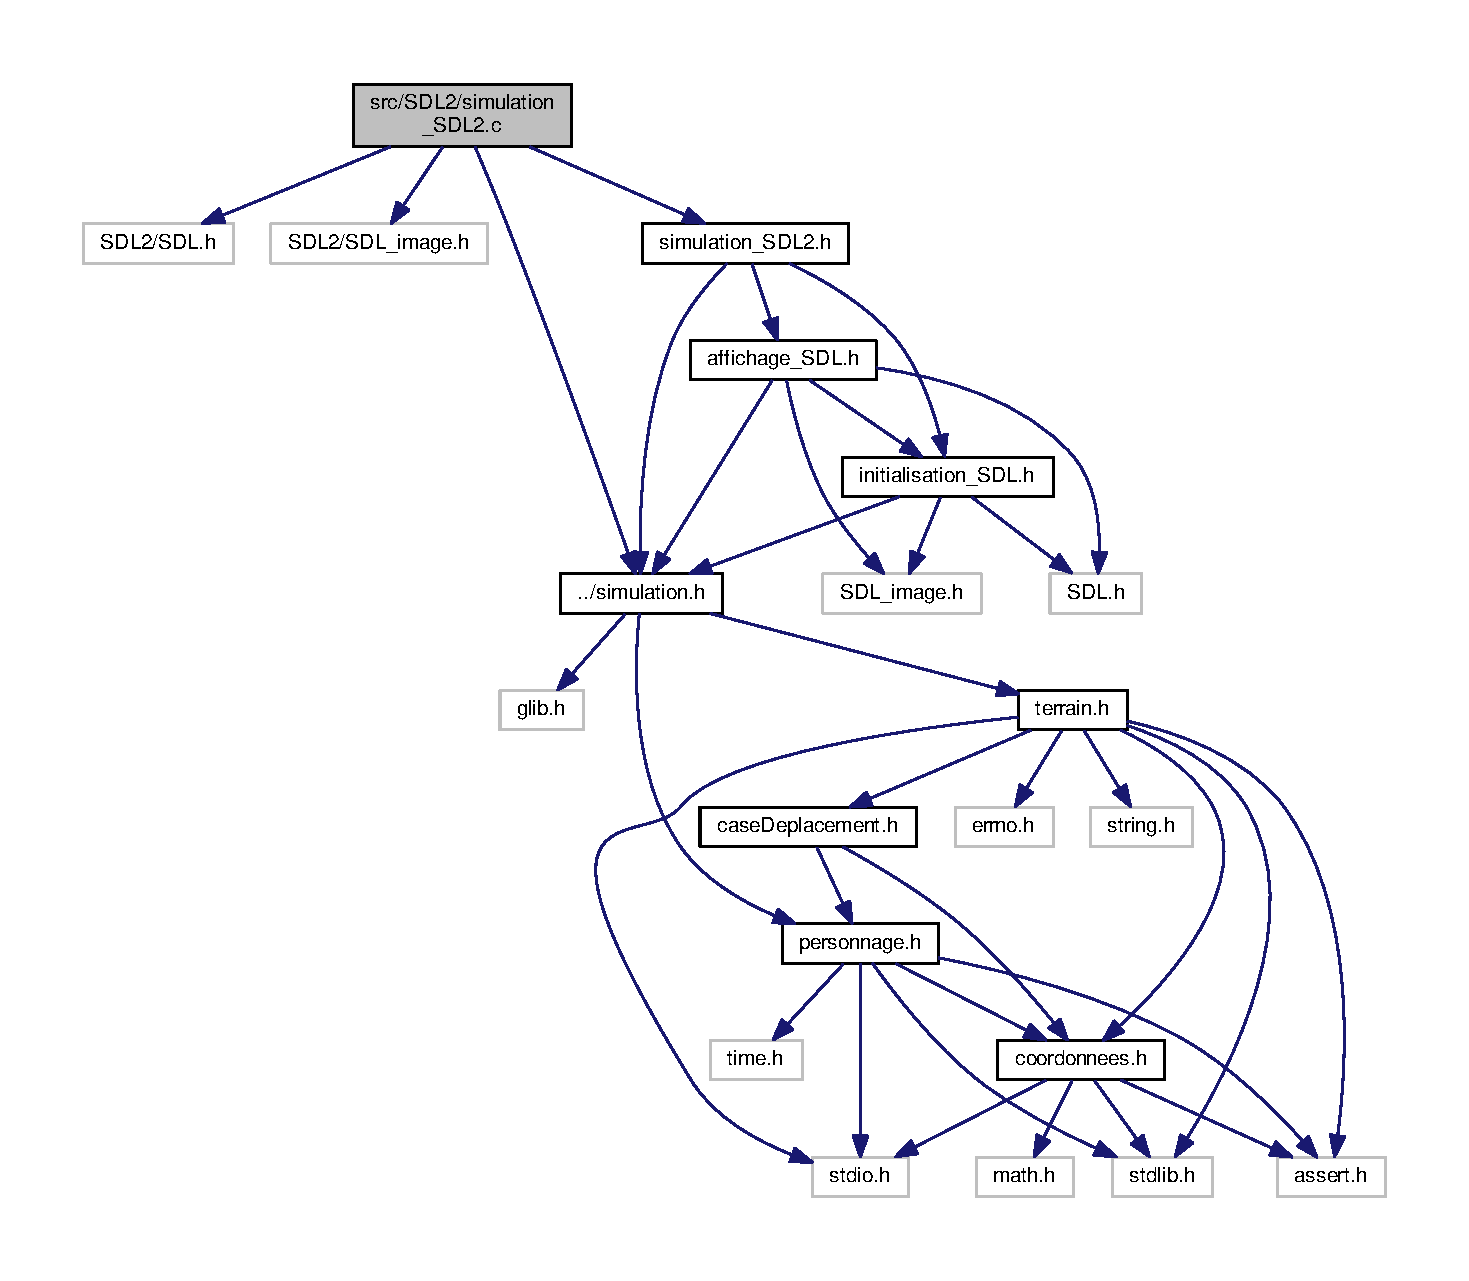
\includegraphics[width=350pt]{simulation__SDL2_8c__incl}
\end{center}
\end{figure}
\subsection*{Fonctions}
\begin{DoxyCompactItemize}
\item 
void \hyperlink{simulation__SDL2_8c_afb9c967cdbed3a77a072a322bbe24a43}{Event\+Clavier} ()
\begin{DoxyCompactList}\small\item\em Fontion de gestion des Input pour la fenetre de simulation. \end{DoxyCompactList}\item 
void \hyperlink{simulation__SDL2_8c_ad5241980dc477033cd5263958a76b266}{Event\+Clavier\+Editeur} (\hyperlink{terrain_8h_a11bbfdc6f8212f3246205cc0e7134136}{Terrain} $\ast$p\+Terrain, char $\ast$chemin\+Fichier)
\begin{DoxyCompactList}\small\item\em Fontion de gestion des Input pour la fenetre de l\textquotesingle{}éditeur. \end{DoxyCompactList}\item 
void \hyperlink{simulation__SDL2_8c_abcc16ac75e4df54756c479fcc310d641}{lancer\+Simulation\+S\+D\+L2} (\hyperlink{simulation_8h_a1ab3bf4791ab776bb4bd460dcce3e8d7}{Simulation} $\ast$p\+Sim)
\begin{DoxyCompactList}\small\item\em Fait tourner toutes les phases de la simulation et lance les fontions d\textquotesingle{}affichage. \end{DoxyCompactList}\item 
void \hyperlink{simulation__SDL2_8c_ac0a9bd316d37dcf65866c261d2d7a970}{lancer\+Simulation\+S\+D\+L2\+Editeur} (char $\ast$chemin\+Fichier, int dimX, int dimY)
\begin{DoxyCompactList}\small\item\em Fait tourner les fonction de l\textquotesingle{}éditeur de niveau et lance les fonctions d\textquotesingle{}affichage de celui-\/ci. \end{DoxyCompactList}\end{DoxyCompactItemize}


\subsection{Documentation des fonctions}
\index{simulation\+\_\+\+S\+D\+L2.\+c@{simulation\+\_\+\+S\+D\+L2.\+c}!Event\+Clavier@{Event\+Clavier}}
\index{Event\+Clavier@{Event\+Clavier}!simulation\+\_\+\+S\+D\+L2.\+c@{simulation\+\_\+\+S\+D\+L2.\+c}}
\subsubsection[{\texorpdfstring{Event\+Clavier()}{EventClavier()}}]{\setlength{\rightskip}{0pt plus 5cm}void Event\+Clavier (
\begin{DoxyParamCaption}
{}
\end{DoxyParamCaption}
)}\hypertarget{simulation__SDL2_8c_afb9c967cdbed3a77a072a322bbe24a43}{}\label{simulation__SDL2_8c_afb9c967cdbed3a77a072a322bbe24a43}


Fontion de gestion des Input pour la fenetre de simulation. 

\index{simulation\+\_\+\+S\+D\+L2.\+c@{simulation\+\_\+\+S\+D\+L2.\+c}!Event\+Clavier\+Editeur@{Event\+Clavier\+Editeur}}
\index{Event\+Clavier\+Editeur@{Event\+Clavier\+Editeur}!simulation\+\_\+\+S\+D\+L2.\+c@{simulation\+\_\+\+S\+D\+L2.\+c}}
\subsubsection[{\texorpdfstring{Event\+Clavier\+Editeur(\+Terrain $\ast$p\+Terrain, char $\ast$chemin\+Fichier)}{EventClavierEditeur(Terrain *pTerrain, char *cheminFichier)}}]{\setlength{\rightskip}{0pt plus 5cm}void Event\+Clavier\+Editeur (
\begin{DoxyParamCaption}
\item[{{\bf Terrain} $\ast$}]{p\+Terrain, }
\item[{char $\ast$}]{chemin\+Fichier}
\end{DoxyParamCaption}
)}\hypertarget{simulation__SDL2_8c_ad5241980dc477033cd5263958a76b266}{}\label{simulation__SDL2_8c_ad5241980dc477033cd5263958a76b266}


Fontion de gestion des Input pour la fenetre de l\textquotesingle{}éditeur. 

\index{simulation\+\_\+\+S\+D\+L2.\+c@{simulation\+\_\+\+S\+D\+L2.\+c}!lancer\+Simulation\+S\+D\+L2@{lancer\+Simulation\+S\+D\+L2}}
\index{lancer\+Simulation\+S\+D\+L2@{lancer\+Simulation\+S\+D\+L2}!simulation\+\_\+\+S\+D\+L2.\+c@{simulation\+\_\+\+S\+D\+L2.\+c}}
\subsubsection[{\texorpdfstring{lancer\+Simulation\+S\+D\+L2(\+Simulation $\ast$p\+Sim)}{lancerSimulationSDL2(Simulation *pSim)}}]{\setlength{\rightskip}{0pt plus 5cm}void lancer\+Simulation\+S\+D\+L2 (
\begin{DoxyParamCaption}
\item[{{\bf Simulation} $\ast$}]{p\+Sim}
\end{DoxyParamCaption}
)}\hypertarget{simulation__SDL2_8c_abcc16ac75e4df54756c479fcc310d641}{}\label{simulation__SDL2_8c_abcc16ac75e4df54756c479fcc310d641}


Fait tourner toutes les phases de la simulation et lance les fontions d\textquotesingle{}affichage. 


\begin{DoxyParams}{Paramètres}
{\em p\+Sim} & Pointeur vers la simulation à lancer dans Sdl \\
\hline
\end{DoxyParams}
\index{simulation\+\_\+\+S\+D\+L2.\+c@{simulation\+\_\+\+S\+D\+L2.\+c}!lancer\+Simulation\+S\+D\+L2\+Editeur@{lancer\+Simulation\+S\+D\+L2\+Editeur}}
\index{lancer\+Simulation\+S\+D\+L2\+Editeur@{lancer\+Simulation\+S\+D\+L2\+Editeur}!simulation\+\_\+\+S\+D\+L2.\+c@{simulation\+\_\+\+S\+D\+L2.\+c}}
\subsubsection[{\texorpdfstring{lancer\+Simulation\+S\+D\+L2\+Editeur(char $\ast$chemin\+Fichier, int dim\+X, int dim\+Y)}{lancerSimulationSDL2Editeur(char *cheminFichier, int dimX, int dimY)}}]{\setlength{\rightskip}{0pt plus 5cm}void lancer\+Simulation\+S\+D\+L2\+Editeur (
\begin{DoxyParamCaption}
\item[{char $\ast$}]{chemin\+Fichier, }
\item[{int}]{dimX, }
\item[{int}]{dimY}
\end{DoxyParamCaption}
)}\hypertarget{simulation__SDL2_8c_ac0a9bd316d37dcf65866c261d2d7a970}{}\label{simulation__SDL2_8c_ac0a9bd316d37dcf65866c261d2d7a970}


Fait tourner les fonction de l\textquotesingle{}éditeur de niveau et lance les fonctions d\textquotesingle{}affichage de celui-\/ci. 


\hypertarget{simulation__SDL2_8h}{}\section{Référence du fichier src/\+S\+D\+L2/simulation\+\_\+\+S\+D\+L2.h}
\label{simulation__SDL2_8h}\index{src/\+S\+D\+L2/simulation\+\_\+\+S\+D\+L2.\+h@{src/\+S\+D\+L2/simulation\+\_\+\+S\+D\+L2.\+h}}


Définit les boucles de de la simulation sous S\+DL.  


{\ttfamily \#include \char`\"{}../simulation.\+h\char`\"{}}\\*
{\ttfamily \#include \char`\"{}initialisation\+\_\+\+S\+D\+L.\+h\char`\"{}}\\*
{\ttfamily \#include \char`\"{}affichage\+\_\+\+S\+D\+L.\+h\char`\"{}}\\*
Graphe des dépendances par inclusion de simulation\+\_\+\+S\+D\+L2.\+h\+:
\nopagebreak
\begin{figure}[H]
\begin{center}
\leavevmode
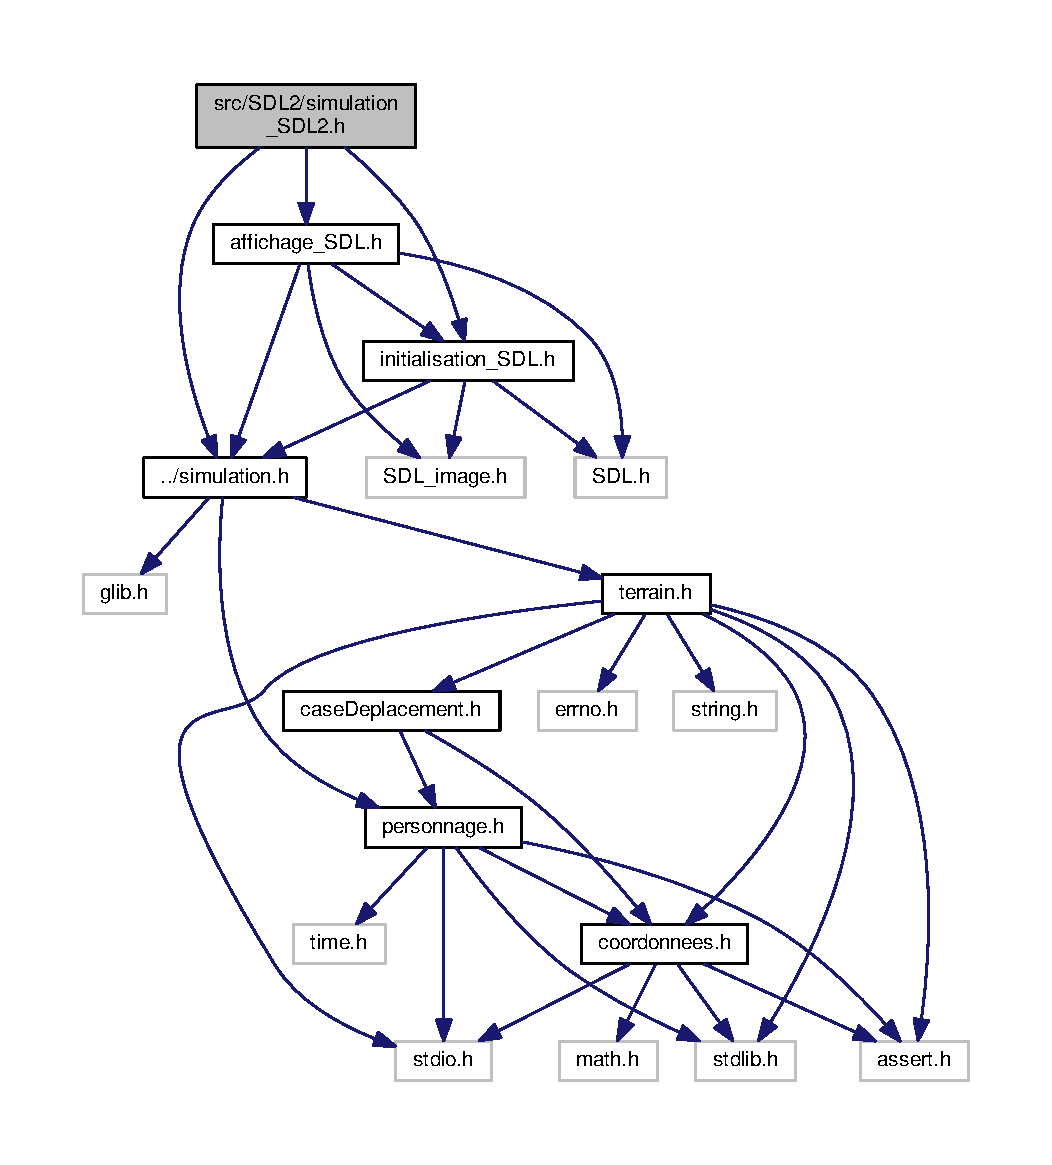
\includegraphics[width=350pt]{simulation__SDL2_8h__incl}
\end{center}
\end{figure}
Ce graphe montre quels fichiers incluent directement ou indirectement ce fichier \+:
\nopagebreak
\begin{figure}[H]
\begin{center}
\leavevmode
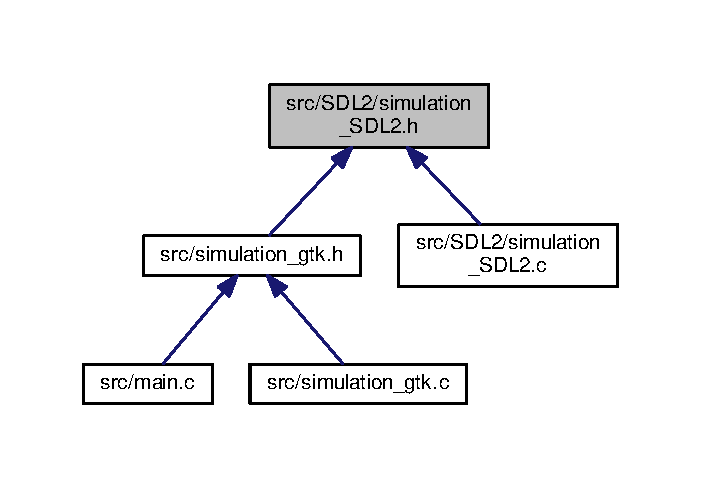
\includegraphics[width=337pt]{simulation__SDL2_8h__dep__incl}
\end{center}
\end{figure}
\subsection*{Fonctions}
\begin{DoxyCompactItemize}
\item 
void \hyperlink{simulation__SDL2_8h_afb9c967cdbed3a77a072a322bbe24a43}{Event\+Clavier} ()
\begin{DoxyCompactList}\small\item\em Fontion de gestion des Input pour la fenetre de simulation. \end{DoxyCompactList}\item 
void \hyperlink{simulation__SDL2_8h_a4d16ef239b37b08bd4145ecb39484f29}{Event\+Clavier\+Editeur} (\hyperlink{terrain_8h_a11bbfdc6f8212f3246205cc0e7134136}{Terrain} $\ast$p\+Terrain, char $\ast$nom\+Terrain)
\begin{DoxyCompactList}\small\item\em Fontion de gestion des Input pour la fenetre de l\textquotesingle{}éditeur. \end{DoxyCompactList}\item 
void \hyperlink{simulation__SDL2_8h_abcc16ac75e4df54756c479fcc310d641}{lancer\+Simulation\+S\+D\+L2} (\hyperlink{simulation_8h_a1ab3bf4791ab776bb4bd460dcce3e8d7}{Simulation} $\ast$p\+Sim)
\begin{DoxyCompactList}\small\item\em Fait tourner toutes les phases de la simulation et lance les fontions d\textquotesingle{}affichage. \end{DoxyCompactList}\item 
void \hyperlink{simulation__SDL2_8h_ac0a9bd316d37dcf65866c261d2d7a970}{lancer\+Simulation\+S\+D\+L2\+Editeur} (char $\ast$chemin\+Fichier, int dimX, int dimY)
\begin{DoxyCompactList}\small\item\em Fait tourner les fonction de l\textquotesingle{}éditeur de niveau et lance les fonctions d\textquotesingle{}affichage de celui-\/ci. \end{DoxyCompactList}\end{DoxyCompactItemize}


\subsection{Description détaillée}
Définit les boucles de de la simulation sous S\+DL. 



\subsection{Documentation des fonctions}
\index{simulation\+\_\+\+S\+D\+L2.\+h@{simulation\+\_\+\+S\+D\+L2.\+h}!Event\+Clavier@{Event\+Clavier}}
\index{Event\+Clavier@{Event\+Clavier}!simulation\+\_\+\+S\+D\+L2.\+h@{simulation\+\_\+\+S\+D\+L2.\+h}}
\subsubsection[{\texorpdfstring{Event\+Clavier()}{EventClavier()}}]{\setlength{\rightskip}{0pt plus 5cm}void Event\+Clavier (
\begin{DoxyParamCaption}
{}
\end{DoxyParamCaption}
)}\hypertarget{simulation__SDL2_8h_afb9c967cdbed3a77a072a322bbe24a43}{}\label{simulation__SDL2_8h_afb9c967cdbed3a77a072a322bbe24a43}


Fontion de gestion des Input pour la fenetre de simulation. 

\index{simulation\+\_\+\+S\+D\+L2.\+h@{simulation\+\_\+\+S\+D\+L2.\+h}!Event\+Clavier\+Editeur@{Event\+Clavier\+Editeur}}
\index{Event\+Clavier\+Editeur@{Event\+Clavier\+Editeur}!simulation\+\_\+\+S\+D\+L2.\+h@{simulation\+\_\+\+S\+D\+L2.\+h}}
\subsubsection[{\texorpdfstring{Event\+Clavier\+Editeur(\+Terrain $\ast$p\+Terrain, char $\ast$nom\+Terrain)}{EventClavierEditeur(Terrain *pTerrain, char *nomTerrain)}}]{\setlength{\rightskip}{0pt plus 5cm}void Event\+Clavier\+Editeur (
\begin{DoxyParamCaption}
\item[{{\bf Terrain} $\ast$}]{p\+Terrain, }
\item[{char $\ast$}]{nom\+Terrain}
\end{DoxyParamCaption}
)}\hypertarget{simulation__SDL2_8h_a4d16ef239b37b08bd4145ecb39484f29}{}\label{simulation__SDL2_8h_a4d16ef239b37b08bd4145ecb39484f29}


Fontion de gestion des Input pour la fenetre de l\textquotesingle{}éditeur. 

\index{simulation\+\_\+\+S\+D\+L2.\+h@{simulation\+\_\+\+S\+D\+L2.\+h}!lancer\+Simulation\+S\+D\+L2@{lancer\+Simulation\+S\+D\+L2}}
\index{lancer\+Simulation\+S\+D\+L2@{lancer\+Simulation\+S\+D\+L2}!simulation\+\_\+\+S\+D\+L2.\+h@{simulation\+\_\+\+S\+D\+L2.\+h}}
\subsubsection[{\texorpdfstring{lancer\+Simulation\+S\+D\+L2(\+Simulation $\ast$p\+Sim)}{lancerSimulationSDL2(Simulation *pSim)}}]{\setlength{\rightskip}{0pt plus 5cm}void lancer\+Simulation\+S\+D\+L2 (
\begin{DoxyParamCaption}
\item[{{\bf Simulation} $\ast$}]{p\+Sim}
\end{DoxyParamCaption}
)}\hypertarget{simulation__SDL2_8h_abcc16ac75e4df54756c479fcc310d641}{}\label{simulation__SDL2_8h_abcc16ac75e4df54756c479fcc310d641}


Fait tourner toutes les phases de la simulation et lance les fontions d\textquotesingle{}affichage. 


\begin{DoxyParams}{Paramètres}
{\em p\+Sim} & Pointeur vers la simulation à lancer dans Sdl \\
\hline
\end{DoxyParams}
\index{simulation\+\_\+\+S\+D\+L2.\+h@{simulation\+\_\+\+S\+D\+L2.\+h}!lancer\+Simulation\+S\+D\+L2\+Editeur@{lancer\+Simulation\+S\+D\+L2\+Editeur}}
\index{lancer\+Simulation\+S\+D\+L2\+Editeur@{lancer\+Simulation\+S\+D\+L2\+Editeur}!simulation\+\_\+\+S\+D\+L2.\+h@{simulation\+\_\+\+S\+D\+L2.\+h}}
\subsubsection[{\texorpdfstring{lancer\+Simulation\+S\+D\+L2\+Editeur(char $\ast$chemin\+Fichier, int dim\+X, int dim\+Y)}{lancerSimulationSDL2Editeur(char *cheminFichier, int dimX, int dimY)}}]{\setlength{\rightskip}{0pt plus 5cm}void lancer\+Simulation\+S\+D\+L2\+Editeur (
\begin{DoxyParamCaption}
\item[{char $\ast$}]{chemin\+Fichier, }
\item[{int}]{dimX, }
\item[{int}]{dimY}
\end{DoxyParamCaption}
)}\hypertarget{simulation__SDL2_8h_ac0a9bd316d37dcf65866c261d2d7a970}{}\label{simulation__SDL2_8h_ac0a9bd316d37dcf65866c261d2d7a970}


Fait tourner les fonction de l\textquotesingle{}éditeur de niveau et lance les fonctions d\textquotesingle{}affichage de celui-\/ci. 


\hypertarget{simulation_8c}{}\section{Référence du fichier src/simulation.c}
\label{simulation_8c}\index{src/simulation.\+c@{src/simulation.\+c}}
{\ttfamily \#include \char`\"{}simulation.\+h\char`\"{}}\\*
Graphe des dépendances par inclusion de simulation.\+c\+:\nopagebreak
\begin{figure}[H]
\begin{center}
\leavevmode
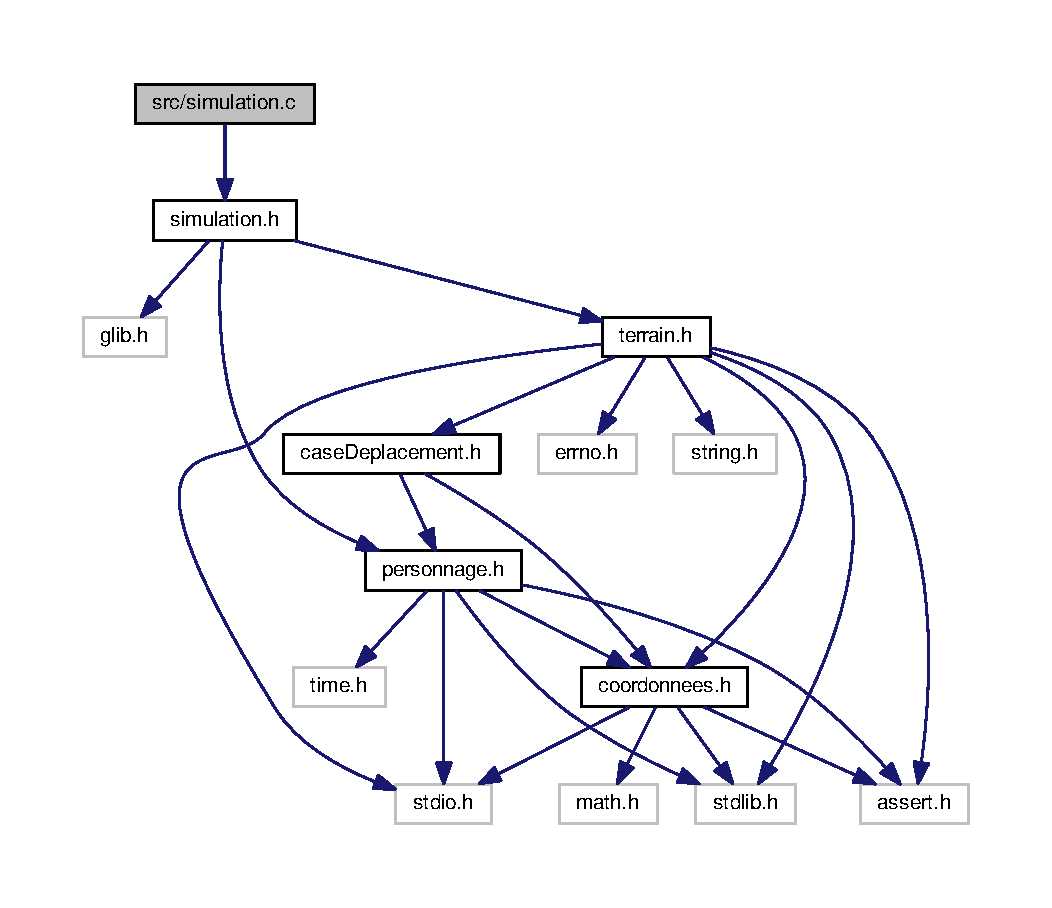
\includegraphics[width=350pt]{simulation_8c__incl}
\end{center}
\end{figure}
\subsection*{Fonctions}
\begin{DoxyCompactItemize}
\item 
\hyperlink{terrain_8h_a11bbfdc6f8212f3246205cc0e7134136}{Terrain} $\ast$ \hyperlink{simulation_8c_a7514376cebf0812d1c64d138766810d5}{get\+Terrain\+\_\+sim} (\hyperlink{simulation_8h_a1ab3bf4791ab776bb4bd460dcce3e8d7}{Simulation} $\ast$p\+Sim)
\begin{DoxyCompactList}\small\item\em Recupère le terrain associé à une Simulation. \end{DoxyCompactList}\item 
void \hyperlink{simulation_8c_ab7d79e2257d2803b99553bf174458c20}{set\+Terrain\+\_\+sim} (\hyperlink{terrain_8h_a11bbfdc6f8212f3246205cc0e7134136}{Terrain} $\ast$p\+Terrain, \hyperlink{simulation_8h_a1ab3bf4791ab776bb4bd460dcce3e8d7}{Simulation} $\ast$p\+Sim)
\item 
int \hyperlink{simulation_8c_a7c69cabd6bffbe631bd22d1d56e680a4}{get\+Nb\+Zombies\+\_\+sim} (\hyperlink{simulation_8h_a1ab3bf4791ab776bb4bd460dcce3e8d7}{Simulation} $\ast$p\+Sim)
\begin{DoxyCompactList}\small\item\em Recupère le nombre de zombie associé à une Simulation. \end{DoxyCompactList}\item 
int \hyperlink{simulation_8c_a9c811803ecb03ac907db8c2d5aa75c4a}{get\+Nb\+Citoyens\+\_\+sim} (\hyperlink{simulation_8h_a1ab3bf4791ab776bb4bd460dcce3e8d7}{Simulation} $\ast$p\+Sim)
\begin{DoxyCompactList}\small\item\em Recupère le nombre de Citoyens associé à une Simulation. \end{DoxyCompactList}\item 
int \hyperlink{simulation_8c_a71bd9dc4548a25fcaa7059e72e0850d2}{get\+Nb\+Policiers\+\_\+sim} (\hyperlink{simulation_8h_a1ab3bf4791ab776bb4bd460dcce3e8d7}{Simulation} $\ast$p\+Sim)
\begin{DoxyCompactList}\small\item\em Recupère le nombre de Policiers associé à une Simulation. \end{DoxyCompactList}\item 
G\+Array $\ast$ \hyperlink{simulation_8c_aba7706e2cab7f8e20c98eaf6269fbdd8}{get\+Zombies\+\_\+sim} (\hyperlink{simulation_8h_a1ab3bf4791ab776bb4bd460dcce3e8d7}{Simulation} $\ast$p\+Sim)
\begin{DoxyCompactList}\small\item\em Recupère la grille de zombie associé à une Simulation. \end{DoxyCompactList}\item 
G\+Array $\ast$ \hyperlink{simulation_8c_a99b58cb2a89463b72b621aae2cc5c956}{get\+Citoyens\+\_\+sim} (\hyperlink{simulation_8h_a1ab3bf4791ab776bb4bd460dcce3e8d7}{Simulation} $\ast$p\+Sim)
\begin{DoxyCompactList}\small\item\em Recupère la grille de Citoyens associé à une Simulation. \end{DoxyCompactList}\item 
G\+Array $\ast$ \hyperlink{simulation_8c_a99c022a1fc4be8ea72049ed8548867cd}{get\+Policiers\+\_\+sim} (\hyperlink{simulation_8h_a1ab3bf4791ab776bb4bd460dcce3e8d7}{Simulation} $\ast$p\+Sim)
\begin{DoxyCompactList}\small\item\em Recupère la grille de Policiers associé à une Simulation. \end{DoxyCompactList}\item 
void \hyperlink{simulation_8c_a44bfaa453f2d4a9cf897235adf4e0c9c}{zombies\+Init\+\_\+sim} (int nb\+Zombies, \hyperlink{simulation_8h_a1ab3bf4791ab776bb4bd460dcce3e8d7}{Simulation} $\ast$p\+Sim)
\begin{DoxyCompactList}\small\item\em Initialise la simulation avec un nombre de zombies. \end{DoxyCompactList}\item 
void \hyperlink{simulation_8c_aaa2bef8ef03449698a1c49f75e8f96bd}{citoyens\+Init\+\_\+sim} (int nb\+Citoyens, \hyperlink{simulation_8h_a1ab3bf4791ab776bb4bd460dcce3e8d7}{Simulation} $\ast$p\+Sim)
\begin{DoxyCompactList}\small\item\em Initialise la simulation avec un nombre de Citoyens. \end{DoxyCompactList}\item 
void \hyperlink{simulation_8c_a846fbbc98362da744d48198158e2d347}{policiers\+Init\+\_\+sim} (int nb\+Policiers, \hyperlink{simulation_8h_a1ab3bf4791ab776bb4bd460dcce3e8d7}{Simulation} $\ast$p\+Sim)
\begin{DoxyCompactList}\small\item\em Initialise la simulation avec un nombre de Policier. \end{DoxyCompactList}\item 
void \hyperlink{simulation_8c_a4099b743564c53f0a937d6d78c48e6e7}{terrain\+Init\+\_\+sim} (char $\ast$nom\+Fic, \hyperlink{simulation_8h_a1ab3bf4791ab776bb4bd460dcce3e8d7}{Simulation} $\ast$p\+Sim)
\begin{DoxyCompactList}\small\item\em Initialise la simulation avec le fichier de nom spécifié \end{DoxyCompactList}\item 
void \hyperlink{simulation_8c_a4c324ae40dcaa9137342cbd93f457184}{init\+Simulation\+\_\+sim} (\hyperlink{simulation_8h_a1ab3bf4791ab776bb4bd460dcce3e8d7}{Simulation} $\ast$p\+Sim, int nb\+Zombies, int nb\+Policiers, int nb\+Citoyens, char $\ast$nom\+Fic)
\begin{DoxyCompactList}\small\item\em Initialise la simulation avec le fichier de nom spécifié, le nombre de zombies, de citoyens et de policier, en appelant les fonctions spécifiques. \end{DoxyCompactList}\item 
\hyperlink{simulation_8h_a1ab3bf4791ab776bb4bd460dcce3e8d7}{Simulation} $\ast$ \hyperlink{simulation_8c_adb815f5c273f29d5e514c2120816a4bd}{creer\+Simulation\+\_\+sim} (int nb\+Zombies, int nb\+Policiers, int nb\+Citoyens, char $\ast$nom\+Fic)
\begin{DoxyCompactList}\small\item\em Creer la simulation avec le fichier de nom spécifié, le nombre de zombies, de citoyens et de policier, en appelant les fonctions spécifiques, et l\textquotesingle{}initialise. \end{DoxyCompactList}\item 
void \hyperlink{simulation_8c_ac03df409b89cfbf5207fe754bc6e670f}{testament\+Sim} (\hyperlink{simulation_8h_a1ab3bf4791ab776bb4bd460dcce3e8d7}{Simulation} $\ast$p\+Sim)
\item 
void \hyperlink{simulation_8c_a4fc35a43279496971fef75d940492f7b}{ajouter\+Perso} (\hyperlink{coordonnees_8h_a79929cdfee7bd985a5e4e25276bb3ba9}{Coordonnees} $\ast$p\+Coord, enum \hyperlink{personnage_8h_a3f6a2951aa3d5d428dd6d61e74db0d75}{type\+Perso} type, \hyperlink{simulation_8h_a1ab3bf4791ab776bb4bd460dcce3e8d7}{Simulation} $\ast$p\+Sim)
\begin{DoxyCompactList}\small\item\em Ajoute un perso à la simulation et au terrain, selon son type. \end{DoxyCompactList}\item 
void \hyperlink{simulation_8c_a0ed5368338ff9e0871bb0c816135971a}{supprimer\+Perso} (\hyperlink{personnage_8h_abd5c92a453bbf273f753b3f5b99da9e7}{Perso} $\ast$p\+Perso, \hyperlink{simulation_8h_a1ab3bf4791ab776bb4bd460dcce3e8d7}{Simulation} $\ast$p\+Sim)
\begin{DoxyCompactList}\small\item\em Supprime un perso de la simulation et de la case à laquelle il est affecté. Ne libère les coordonnées affectées. \end{DoxyCompactList}\item 
void \hyperlink{simulation_8c_a71d0dfc00495ee18d6a263e93a5cf8dd}{deplacer\+Zombies\+\_\+sim} (\hyperlink{simulation_8h_a1ab3bf4791ab776bb4bd460dcce3e8d7}{Simulation} $\ast$p\+Sim)
\begin{DoxyCompactList}\small\item\em Executes les deplacement des Zombies de manière aléatoire. \end{DoxyCompactList}\item 
void \hyperlink{simulation_8c_a7be1f8001d8bc5edb63625a8fa8df70a}{deplacer\+Citoyens\+\_\+sim} (\hyperlink{simulation_8h_a1ab3bf4791ab776bb4bd460dcce3e8d7}{Simulation} $\ast$p\+Sim)
\begin{DoxyCompactList}\small\item\em Executes les deplacement des Citoyens de manière aléatoire. \end{DoxyCompactList}\item 
void \hyperlink{simulation_8c_af61e27b9f0b0a9c55a56f3af37f90f74}{deplacer\+Policiers\+\_\+sim} (\hyperlink{simulation_8h_a1ab3bf4791ab776bb4bd460dcce3e8d7}{Simulation} $\ast$p\+Sim)
\begin{DoxyCompactList}\small\item\em Executes les deplacement des policiers de manière aléatoire. \end{DoxyCompactList}\item 
void \hyperlink{simulation_8c_a99cf798b51aeb7a2828941fb096a9766}{deplacement\+Intel\+Zombies\+\_\+sim} (\hyperlink{simulation_8h_a1ab3bf4791ab776bb4bd460dcce3e8d7}{Simulation} $\ast$p\+Sim)
\begin{DoxyCompactList}\small\item\em Executes les deplacement des zombies de manière intelligente et en regard des champs. \end{DoxyCompactList}\item 
void \hyperlink{simulation_8c_acc4f40dd69c6516a19a38e065ee3395f}{deplacement\+Intel\+Citoyens\+\_\+sim} (\hyperlink{simulation_8h_a1ab3bf4791ab776bb4bd460dcce3e8d7}{Simulation} $\ast$p\+Sim)
\begin{DoxyCompactList}\small\item\em Executes les deplacement des Citoyens de manière intelligente et en regard des champs. \end{DoxyCompactList}\item 
void \hyperlink{simulation_8c_ab4c303981dc0289a2b211ba3e24ccf55}{deplacement\+Intel\+Policiers\+\_\+sim} (\hyperlink{simulation_8h_a1ab3bf4791ab776bb4bd460dcce3e8d7}{Simulation} $\ast$p\+Sim)
\begin{DoxyCompactList}\small\item\em Executes les deplacement des Policiers de manière intelligente et en regard des champs. \end{DoxyCompactList}\item 
void \hyperlink{simulation_8c_ad1f35ce5f9b80c161777a7e3b8cdee5a}{deplacer\+Perso\+\_\+sim} (\hyperlink{simulation_8h_a1ab3bf4791ab776bb4bd460dcce3e8d7}{Simulation} $\ast$p\+Sim)
\begin{DoxyCompactList}\small\item\em Executes les deplacement des personnages de manière aléatoire. \end{DoxyCompactList}\item 
void \hyperlink{simulation_8c_a8e9f7110fca5097ac2e3b0c5b37549af}{contaminations} (\hyperlink{simulation_8h_a1ab3bf4791ab776bb4bd460dcce3e8d7}{Simulation} $\ast$p\+Sim)
\begin{DoxyCompactList}\small\item\em Executes les instruction de contamination des policier et citoyens par les zombies. \end{DoxyCompactList}\item 
void \hyperlink{simulation_8c_abf7873243ac6158bd5dfac2dc3b376b1}{tirs} (\hyperlink{simulation_8h_a1ab3bf4791ab776bb4bd460dcce3e8d7}{Simulation} $\ast$p\+Sim)
\begin{DoxyCompactList}\small\item\em Executes les instruction de tirs des policiers sur les zombies. \end{DoxyCompactList}\item 
void \hyperlink{simulation_8c_aec9f9a901b4ea316a48612d15e772dfc}{propager\+Champs\+Persos} (\hyperlink{simulation_8h_a1ab3bf4791ab776bb4bd460dcce3e8d7}{Simulation} $\ast$p\+Sim)
\begin{DoxyCompactList}\small\item\em Propage les champs des personnages dans la simulation. \end{DoxyCompactList}\item 
void \hyperlink{simulation_8c_ac61d3c90dafcff499c3ec3d8095c88bb}{deplacement\+Intel\+Zombie} (\hyperlink{personnage_8h_abd5c92a453bbf273f753b3f5b99da9e7}{Perso} $\ast$p\+Perso, \hyperlink{simulation_8h_a1ab3bf4791ab776bb4bd460dcce3e8d7}{Simulation} $\ast$p\+Sim)
\begin{DoxyCompactList}\small\item\em Executes les instruction de deplacement intteligent d\textquotesingle{}un Zombie. \end{DoxyCompactList}\item 
void \hyperlink{simulation_8c_a119206545d9d380e685a18c9987d3856}{deplacement\+Intel\+Citoyen} (\hyperlink{personnage_8h_abd5c92a453bbf273f753b3f5b99da9e7}{Perso} $\ast$p\+Perso, \hyperlink{simulation_8h_a1ab3bf4791ab776bb4bd460dcce3e8d7}{Simulation} $\ast$p\+Sim)
\begin{DoxyCompactList}\small\item\em Executes les instruction de deplacement intteligent d\textquotesingle{}un Citoyen. \end{DoxyCompactList}\item 
void \hyperlink{simulation_8c_abd1af38115336e38d41f0c42123a2024}{deplacement\+Intel\+Policier} (\hyperlink{personnage_8h_abd5c92a453bbf273f753b3f5b99da9e7}{Perso} $\ast$p\+Perso, \hyperlink{simulation_8h_a1ab3bf4791ab776bb4bd460dcce3e8d7}{Simulation} $\ast$p\+Sim)
\begin{DoxyCompactList}\small\item\em Executes les instruction de deplacement intteligent d\textquotesingle{}un Policier. \end{DoxyCompactList}\item 
void \hyperlink{simulation_8c_a8c84b81dbfbacce2c792705198ee9f71}{test\+Fonctions\+\_\+sim} ()
\begin{DoxyCompactList}\small\item\em Focntions de test des fonctions du module Simulation. \end{DoxyCompactList}\item 
int \hyperlink{simulation_8c_a14a4e9bf4982b1fdd2b26a6f82d24fc0}{compare\+Tab2D} (const void $\ast$a, const void $\ast$b)
\begin{DoxyCompactList}\small\item\em Fonction à appeler avec qsort pour trier un tableau 2D en lignes par rapport à la première case. \end{DoxyCompactList}\end{DoxyCompactItemize}


\subsection{Documentation des fonctions}
\index{simulation.\+c@{simulation.\+c}!ajouter\+Perso@{ajouter\+Perso}}
\index{ajouter\+Perso@{ajouter\+Perso}!simulation.\+c@{simulation.\+c}}
\subsubsection[{\texorpdfstring{ajouter\+Perso(\+Coordonnees $\ast$p\+Coord, enum type\+Perso type, Simulation $\ast$p\+Sim)}{ajouterPerso(Coordonnees *pCoord, enum typePerso type, Simulation *pSim)}}]{\setlength{\rightskip}{0pt plus 5cm}void ajouter\+Perso (
\begin{DoxyParamCaption}
\item[{{\bf Coordonnees} $\ast$}]{p\+Coord, }
\item[{enum {\bf type\+Perso}}]{type, }
\item[{{\bf Simulation} $\ast$}]{p\+Sim}
\end{DoxyParamCaption}
)}\hypertarget{simulation_8c_a4fc35a43279496971fef75d940492f7b}{}\label{simulation_8c_a4fc35a43279496971fef75d940492f7b}


Ajoute un perso à la simulation et au terrain, selon son type. 


\begin{DoxyParams}{Paramètres}
{\em p\+Coord} & Coordonnées du personnage sur le terrain \\
\hline
{\em type} & Type du perso (Z\+O\+M\+B\+IE, P\+O\+L\+I\+C\+I\+ER, C\+I\+T\+O\+Y\+EN) \\
\hline
{\em p\+Sim} & Pointeur sur la simulation \\
\hline
\end{DoxyParams}
\index{simulation.\+c@{simulation.\+c}!citoyens\+Init\+\_\+sim@{citoyens\+Init\+\_\+sim}}
\index{citoyens\+Init\+\_\+sim@{citoyens\+Init\+\_\+sim}!simulation.\+c@{simulation.\+c}}
\subsubsection[{\texorpdfstring{citoyens\+Init\+\_\+sim(int nb\+Citoyens, Simulation $\ast$p\+Sim)}{citoyensInit_sim(int nbCitoyens, Simulation *pSim)}}]{\setlength{\rightskip}{0pt plus 5cm}void citoyens\+Init\+\_\+sim (
\begin{DoxyParamCaption}
\item[{int}]{nb\+Citoyens, }
\item[{{\bf Simulation} $\ast$}]{p\+Sim}
\end{DoxyParamCaption}
)}\hypertarget{simulation_8c_aaa2bef8ef03449698a1c49f75e8f96bd}{}\label{simulation_8c_aaa2bef8ef03449698a1c49f75e8f96bd}


Initialise la simulation avec un nombre de Citoyens. 


\begin{DoxyParams}{Paramètres}
{\em nb\+Citoyens} & Nombres de Citoyens a initialiser dans la Simulation \\
\hline
{\em p\+Sim} & La simulation a initialiser \\
\hline
\end{DoxyParams}
\index{simulation.\+c@{simulation.\+c}!compare\+Tab2D@{compare\+Tab2D}}
\index{compare\+Tab2D@{compare\+Tab2D}!simulation.\+c@{simulation.\+c}}
\subsubsection[{\texorpdfstring{compare\+Tab2\+D(const void $\ast$a, const void $\ast$b)}{compareTab2D(const void *a, const void *b)}}]{\setlength{\rightskip}{0pt plus 5cm}int compare\+Tab2D (
\begin{DoxyParamCaption}
\item[{const void $\ast$}]{a, }
\item[{const void $\ast$}]{b}
\end{DoxyParamCaption}
)}\hypertarget{simulation_8c_a14a4e9bf4982b1fdd2b26a6f82d24fc0}{}\label{simulation_8c_a14a4e9bf4982b1fdd2b26a6f82d24fc0}


Fonction à appeler avec qsort pour trier un tableau 2D en lignes par rapport à la première case. 


\begin{DoxyParams}{Paramètres}
{\em a} & Pointeur sur une case du tableau \\
\hline
{\em b} & Pointeur sur une case du tableau \\
\hline
\end{DoxyParams}
\index{simulation.\+c@{simulation.\+c}!contaminations@{contaminations}}
\index{contaminations@{contaminations}!simulation.\+c@{simulation.\+c}}
\subsubsection[{\texorpdfstring{contaminations(\+Simulation $\ast$p\+Sim)}{contaminations(Simulation *pSim)}}]{\setlength{\rightskip}{0pt plus 5cm}void contaminations (
\begin{DoxyParamCaption}
\item[{{\bf Simulation} $\ast$}]{p\+Sim}
\end{DoxyParamCaption}
)}\hypertarget{simulation_8c_a8e9f7110fca5097ac2e3b0c5b37549af}{}\label{simulation_8c_a8e9f7110fca5097ac2e3b0c5b37549af}


Executes les instruction de contamination des policier et citoyens par les zombies. 


\begin{DoxyParams}{Paramètres}
{\em p\+Sim} & La simulation dans laquelle tout est effectué \\
\hline
\end{DoxyParams}
\index{simulation.\+c@{simulation.\+c}!creer\+Simulation\+\_\+sim@{creer\+Simulation\+\_\+sim}}
\index{creer\+Simulation\+\_\+sim@{creer\+Simulation\+\_\+sim}!simulation.\+c@{simulation.\+c}}
\subsubsection[{\texorpdfstring{creer\+Simulation\+\_\+sim(int nb\+Zombies, int nb\+Policiers, int nb\+Citoyens, char $\ast$nom\+Fic)}{creerSimulation_sim(int nbZombies, int nbPoliciers, int nbCitoyens, char *nomFic)}}]{\setlength{\rightskip}{0pt plus 5cm}{\bf Simulation}$\ast$ creer\+Simulation\+\_\+sim (
\begin{DoxyParamCaption}
\item[{int}]{nb\+Zombies, }
\item[{int}]{nb\+Citoyens, }
\item[{int}]{nb\+Policiers, }
\item[{char $\ast$}]{nom\+Fic}
\end{DoxyParamCaption}
)}\hypertarget{simulation_8c_adb815f5c273f29d5e514c2120816a4bd}{}\label{simulation_8c_adb815f5c273f29d5e514c2120816a4bd}


Creer la simulation avec le fichier de nom spécifié, le nombre de zombies, de citoyens et de policier, en appelant les fonctions spécifiques, et l\textquotesingle{}initialise. 


\begin{DoxyParams}{Paramètres}
{\em nb\+Zombies} & Nombres de zombies a creer dans la Simulation \\
\hline
{\em nb\+Citoyens} & Nombres de Citoyens a creer dans la Simulation \\
\hline
{\em nb\+Policiers} & Nombres de Policiers a creer dans la Simulation \\
\hline
{\em nom\+Fic} & Chaine de caractère de nom du fichier \\
\hline
\end{DoxyParams}
\begin{DoxyReturn}{Renvoie}
p\+Sim Pointeur vers la Simulation crée 
\end{DoxyReturn}
\index{simulation.\+c@{simulation.\+c}!deplacement\+Intel\+Citoyen@{deplacement\+Intel\+Citoyen}}
\index{deplacement\+Intel\+Citoyen@{deplacement\+Intel\+Citoyen}!simulation.\+c@{simulation.\+c}}
\subsubsection[{\texorpdfstring{deplacement\+Intel\+Citoyen(\+Perso $\ast$p\+Perso, Simulation $\ast$p\+Sim)}{deplacementIntelCitoyen(Perso *pPerso, Simulation *pSim)}}]{\setlength{\rightskip}{0pt plus 5cm}void deplacement\+Intel\+Citoyen (
\begin{DoxyParamCaption}
\item[{{\bf Perso} $\ast$}]{p\+Perso, }
\item[{{\bf Simulation} $\ast$}]{p\+Sim}
\end{DoxyParamCaption}
)}\hypertarget{simulation_8c_a119206545d9d380e685a18c9987d3856}{}\label{simulation_8c_a119206545d9d380e685a18c9987d3856}


Executes les instruction de deplacement intteligent d\textquotesingle{}un Citoyen. 


\begin{DoxyParams}{Paramètres}
{\em p\+Perso} & Pointeur vers l\textquotesingle{}entité qui va etre déplacé intelligement \\
\hline
{\em p\+Sim} & La simulation dans laquelle tout est effectué \\
\hline
\end{DoxyParams}
\index{simulation.\+c@{simulation.\+c}!deplacement\+Intel\+Citoyens\+\_\+sim@{deplacement\+Intel\+Citoyens\+\_\+sim}}
\index{deplacement\+Intel\+Citoyens\+\_\+sim@{deplacement\+Intel\+Citoyens\+\_\+sim}!simulation.\+c@{simulation.\+c}}
\subsubsection[{\texorpdfstring{deplacement\+Intel\+Citoyens\+\_\+sim(\+Simulation $\ast$p\+Sim)}{deplacementIntelCitoyens_sim(Simulation *pSim)}}]{\setlength{\rightskip}{0pt plus 5cm}void deplacement\+Intel\+Citoyens\+\_\+sim (
\begin{DoxyParamCaption}
\item[{{\bf Simulation} $\ast$}]{p\+Sim}
\end{DoxyParamCaption}
)}\hypertarget{simulation_8c_acc4f40dd69c6516a19a38e065ee3395f}{}\label{simulation_8c_acc4f40dd69c6516a19a38e065ee3395f}


Executes les deplacement des Citoyens de manière intelligente et en regard des champs. 


\begin{DoxyParams}{Paramètres}
{\em p\+Sim} & La simulation dans laquelle tout est effectué \\
\hline
\end{DoxyParams}
\index{simulation.\+c@{simulation.\+c}!deplacement\+Intel\+Policier@{deplacement\+Intel\+Policier}}
\index{deplacement\+Intel\+Policier@{deplacement\+Intel\+Policier}!simulation.\+c@{simulation.\+c}}
\subsubsection[{\texorpdfstring{deplacement\+Intel\+Policier(\+Perso $\ast$p\+Perso, Simulation $\ast$p\+Sim)}{deplacementIntelPolicier(Perso *pPerso, Simulation *pSim)}}]{\setlength{\rightskip}{0pt plus 5cm}void deplacement\+Intel\+Policier (
\begin{DoxyParamCaption}
\item[{{\bf Perso} $\ast$}]{p\+Perso, }
\item[{{\bf Simulation} $\ast$}]{p\+Sim}
\end{DoxyParamCaption}
)}\hypertarget{simulation_8c_abd1af38115336e38d41f0c42123a2024}{}\label{simulation_8c_abd1af38115336e38d41f0c42123a2024}


Executes les instruction de deplacement intteligent d\textquotesingle{}un Policier. 


\begin{DoxyParams}{Paramètres}
{\em p\+Perso} & Pointeur vers l\textquotesingle{}entité qui va etre déplacé intelligement \\
\hline
{\em p\+Sim} & La simulation dans laquelle tout est effectué \\
\hline
\end{DoxyParams}
\index{simulation.\+c@{simulation.\+c}!deplacement\+Intel\+Policiers\+\_\+sim@{deplacement\+Intel\+Policiers\+\_\+sim}}
\index{deplacement\+Intel\+Policiers\+\_\+sim@{deplacement\+Intel\+Policiers\+\_\+sim}!simulation.\+c@{simulation.\+c}}
\subsubsection[{\texorpdfstring{deplacement\+Intel\+Policiers\+\_\+sim(\+Simulation $\ast$p\+Sim)}{deplacementIntelPoliciers_sim(Simulation *pSim)}}]{\setlength{\rightskip}{0pt plus 5cm}void deplacement\+Intel\+Policiers\+\_\+sim (
\begin{DoxyParamCaption}
\item[{{\bf Simulation} $\ast$}]{p\+Sim}
\end{DoxyParamCaption}
)}\hypertarget{simulation_8c_ab4c303981dc0289a2b211ba3e24ccf55}{}\label{simulation_8c_ab4c303981dc0289a2b211ba3e24ccf55}


Executes les deplacement des Policiers de manière intelligente et en regard des champs. 


\begin{DoxyParams}{Paramètres}
{\em p\+Sim} & La simulation dans laquelle tout est effectué \\
\hline
\end{DoxyParams}
\index{simulation.\+c@{simulation.\+c}!deplacement\+Intel\+Zombie@{deplacement\+Intel\+Zombie}}
\index{deplacement\+Intel\+Zombie@{deplacement\+Intel\+Zombie}!simulation.\+c@{simulation.\+c}}
\subsubsection[{\texorpdfstring{deplacement\+Intel\+Zombie(\+Perso $\ast$p\+Perso, Simulation $\ast$p\+Sim)}{deplacementIntelZombie(Perso *pPerso, Simulation *pSim)}}]{\setlength{\rightskip}{0pt plus 5cm}void deplacement\+Intel\+Zombie (
\begin{DoxyParamCaption}
\item[{{\bf Perso} $\ast$}]{p\+Perso, }
\item[{{\bf Simulation} $\ast$}]{p\+Sim}
\end{DoxyParamCaption}
)}\hypertarget{simulation_8c_ac61d3c90dafcff499c3ec3d8095c88bb}{}\label{simulation_8c_ac61d3c90dafcff499c3ec3d8095c88bb}


Executes les instruction de deplacement intteligent d\textquotesingle{}un Zombie. 


\begin{DoxyParams}{Paramètres}
{\em p\+Perso} & Pointeur vers l\textquotesingle{}entité qui va etre déplacé intelligement \\
\hline
{\em p\+Sim} & La simulation dans laquelle tout est effectué \\
\hline
\end{DoxyParams}
\index{simulation.\+c@{simulation.\+c}!deplacement\+Intel\+Zombies\+\_\+sim@{deplacement\+Intel\+Zombies\+\_\+sim}}
\index{deplacement\+Intel\+Zombies\+\_\+sim@{deplacement\+Intel\+Zombies\+\_\+sim}!simulation.\+c@{simulation.\+c}}
\subsubsection[{\texorpdfstring{deplacement\+Intel\+Zombies\+\_\+sim(\+Simulation $\ast$p\+Sim)}{deplacementIntelZombies_sim(Simulation *pSim)}}]{\setlength{\rightskip}{0pt plus 5cm}void deplacement\+Intel\+Zombies\+\_\+sim (
\begin{DoxyParamCaption}
\item[{{\bf Simulation} $\ast$}]{p\+Sim}
\end{DoxyParamCaption}
)}\hypertarget{simulation_8c_a99cf798b51aeb7a2828941fb096a9766}{}\label{simulation_8c_a99cf798b51aeb7a2828941fb096a9766}


Executes les deplacement des zombies de manière intelligente et en regard des champs. 


\begin{DoxyParams}{Paramètres}
{\em p\+Sim} & La simulation dans laquelle tout est effectué \\
\hline
\end{DoxyParams}
\index{simulation.\+c@{simulation.\+c}!deplacer\+Citoyens\+\_\+sim@{deplacer\+Citoyens\+\_\+sim}}
\index{deplacer\+Citoyens\+\_\+sim@{deplacer\+Citoyens\+\_\+sim}!simulation.\+c@{simulation.\+c}}
\subsubsection[{\texorpdfstring{deplacer\+Citoyens\+\_\+sim(\+Simulation $\ast$p\+Sim)}{deplacerCitoyens_sim(Simulation *pSim)}}]{\setlength{\rightskip}{0pt plus 5cm}void deplacer\+Citoyens\+\_\+sim (
\begin{DoxyParamCaption}
\item[{{\bf Simulation} $\ast$}]{p\+Sim}
\end{DoxyParamCaption}
)}\hypertarget{simulation_8c_a7be1f8001d8bc5edb63625a8fa8df70a}{}\label{simulation_8c_a7be1f8001d8bc5edb63625a8fa8df70a}


Executes les deplacement des Citoyens de manière aléatoire. 


\begin{DoxyParams}{Paramètres}
{\em p\+Sim} & La simulation dans laquelle tout est effectué \\
\hline
\end{DoxyParams}
\index{simulation.\+c@{simulation.\+c}!deplacer\+Perso\+\_\+sim@{deplacer\+Perso\+\_\+sim}}
\index{deplacer\+Perso\+\_\+sim@{deplacer\+Perso\+\_\+sim}!simulation.\+c@{simulation.\+c}}
\subsubsection[{\texorpdfstring{deplacer\+Perso\+\_\+sim(\+Simulation $\ast$p\+Sim)}{deplacerPerso_sim(Simulation *pSim)}}]{\setlength{\rightskip}{0pt plus 5cm}void deplacer\+Perso\+\_\+sim (
\begin{DoxyParamCaption}
\item[{{\bf Simulation} $\ast$}]{p\+Sim}
\end{DoxyParamCaption}
)}\hypertarget{simulation_8c_ad1f35ce5f9b80c161777a7e3b8cdee5a}{}\label{simulation_8c_ad1f35ce5f9b80c161777a7e3b8cdee5a}


Executes les deplacement des personnages de manière aléatoire. 


\begin{DoxyParams}{Paramètres}
{\em p\+Sim} & La simulation dans laquelle tout est effectué \\
\hline
\end{DoxyParams}
\index{simulation.\+c@{simulation.\+c}!deplacer\+Policiers\+\_\+sim@{deplacer\+Policiers\+\_\+sim}}
\index{deplacer\+Policiers\+\_\+sim@{deplacer\+Policiers\+\_\+sim}!simulation.\+c@{simulation.\+c}}
\subsubsection[{\texorpdfstring{deplacer\+Policiers\+\_\+sim(\+Simulation $\ast$p\+Sim)}{deplacerPoliciers_sim(Simulation *pSim)}}]{\setlength{\rightskip}{0pt plus 5cm}void deplacer\+Policiers\+\_\+sim (
\begin{DoxyParamCaption}
\item[{{\bf Simulation} $\ast$}]{p\+Sim}
\end{DoxyParamCaption}
)}\hypertarget{simulation_8c_af61e27b9f0b0a9c55a56f3af37f90f74}{}\label{simulation_8c_af61e27b9f0b0a9c55a56f3af37f90f74}


Executes les deplacement des policiers de manière aléatoire. 


\begin{DoxyParams}{Paramètres}
{\em p\+Sim} & La simulation dans laquelle tout est effectué \\
\hline
\end{DoxyParams}
\index{simulation.\+c@{simulation.\+c}!deplacer\+Zombies\+\_\+sim@{deplacer\+Zombies\+\_\+sim}}
\index{deplacer\+Zombies\+\_\+sim@{deplacer\+Zombies\+\_\+sim}!simulation.\+c@{simulation.\+c}}
\subsubsection[{\texorpdfstring{deplacer\+Zombies\+\_\+sim(\+Simulation $\ast$p\+Sim)}{deplacerZombies_sim(Simulation *pSim)}}]{\setlength{\rightskip}{0pt plus 5cm}void deplacer\+Zombies\+\_\+sim (
\begin{DoxyParamCaption}
\item[{{\bf Simulation} $\ast$}]{p\+Sim}
\end{DoxyParamCaption}
)}\hypertarget{simulation_8c_a71d0dfc00495ee18d6a263e93a5cf8dd}{}\label{simulation_8c_a71d0dfc00495ee18d6a263e93a5cf8dd}


Executes les deplacement des Zombies de manière aléatoire. 


\begin{DoxyParams}{Paramètres}
{\em p\+Sim} & La simulation dans laquelle tout est effectué \\
\hline
\end{DoxyParams}
\index{simulation.\+c@{simulation.\+c}!get\+Citoyens\+\_\+sim@{get\+Citoyens\+\_\+sim}}
\index{get\+Citoyens\+\_\+sim@{get\+Citoyens\+\_\+sim}!simulation.\+c@{simulation.\+c}}
\subsubsection[{\texorpdfstring{get\+Citoyens\+\_\+sim(\+Simulation $\ast$p\+Sim)}{getCitoyens_sim(Simulation *pSim)}}]{\setlength{\rightskip}{0pt plus 5cm}G\+Array$\ast$ get\+Citoyens\+\_\+sim (
\begin{DoxyParamCaption}
\item[{{\bf Simulation} $\ast$}]{p\+Sim}
\end{DoxyParamCaption}
)}\hypertarget{simulation_8c_a99b58cb2a89463b72b621aae2cc5c956}{}\label{simulation_8c_a99b58cb2a89463b72b621aae2cc5c956}


Recupère la grille de Citoyens associé à une Simulation. 


\begin{DoxyParams}{Paramètres}
{\em p\+Sim} & La simulation a étudier \\
\hline
\end{DoxyParams}
\begin{DoxyReturn}{Renvoie}
Pointeur vers la grille de Citoyens 
\end{DoxyReturn}
\index{simulation.\+c@{simulation.\+c}!get\+Nb\+Citoyens\+\_\+sim@{get\+Nb\+Citoyens\+\_\+sim}}
\index{get\+Nb\+Citoyens\+\_\+sim@{get\+Nb\+Citoyens\+\_\+sim}!simulation.\+c@{simulation.\+c}}
\subsubsection[{\texorpdfstring{get\+Nb\+Citoyens\+\_\+sim(\+Simulation $\ast$p\+Sim)}{getNbCitoyens_sim(Simulation *pSim)}}]{\setlength{\rightskip}{0pt plus 5cm}int get\+Nb\+Citoyens\+\_\+sim (
\begin{DoxyParamCaption}
\item[{{\bf Simulation} $\ast$}]{p\+Sim}
\end{DoxyParamCaption}
)}\hypertarget{simulation_8c_a9c811803ecb03ac907db8c2d5aa75c4a}{}\label{simulation_8c_a9c811803ecb03ac907db8c2d5aa75c4a}


Recupère le nombre de Citoyens associé à une Simulation. 


\begin{DoxyParams}{Paramètres}
{\em p\+Sim} & La simulation a étudier \\
\hline
\end{DoxyParams}
\begin{DoxyReturn}{Renvoie}
Entier du nombre de Citoyens dans la Simulation 
\end{DoxyReturn}
\index{simulation.\+c@{simulation.\+c}!get\+Nb\+Policiers\+\_\+sim@{get\+Nb\+Policiers\+\_\+sim}}
\index{get\+Nb\+Policiers\+\_\+sim@{get\+Nb\+Policiers\+\_\+sim}!simulation.\+c@{simulation.\+c}}
\subsubsection[{\texorpdfstring{get\+Nb\+Policiers\+\_\+sim(\+Simulation $\ast$p\+Sim)}{getNbPoliciers_sim(Simulation *pSim)}}]{\setlength{\rightskip}{0pt plus 5cm}int get\+Nb\+Policiers\+\_\+sim (
\begin{DoxyParamCaption}
\item[{{\bf Simulation} $\ast$}]{p\+Sim}
\end{DoxyParamCaption}
)}\hypertarget{simulation_8c_a71bd9dc4548a25fcaa7059e72e0850d2}{}\label{simulation_8c_a71bd9dc4548a25fcaa7059e72e0850d2}


Recupère le nombre de Policiers associé à une Simulation. 


\begin{DoxyParams}{Paramètres}
{\em p\+Sim} & La simulation a étudier \\
\hline
\end{DoxyParams}
\begin{DoxyReturn}{Renvoie}
Entier du nombre de Policiers dans la Simulation 
\end{DoxyReturn}
\index{simulation.\+c@{simulation.\+c}!get\+Nb\+Zombies\+\_\+sim@{get\+Nb\+Zombies\+\_\+sim}}
\index{get\+Nb\+Zombies\+\_\+sim@{get\+Nb\+Zombies\+\_\+sim}!simulation.\+c@{simulation.\+c}}
\subsubsection[{\texorpdfstring{get\+Nb\+Zombies\+\_\+sim(\+Simulation $\ast$p\+Sim)}{getNbZombies_sim(Simulation *pSim)}}]{\setlength{\rightskip}{0pt plus 5cm}int get\+Nb\+Zombies\+\_\+sim (
\begin{DoxyParamCaption}
\item[{{\bf Simulation} $\ast$}]{p\+Sim}
\end{DoxyParamCaption}
)}\hypertarget{simulation_8c_a7c69cabd6bffbe631bd22d1d56e680a4}{}\label{simulation_8c_a7c69cabd6bffbe631bd22d1d56e680a4}


Recupère le nombre de zombie associé à une Simulation. 


\begin{DoxyParams}{Paramètres}
{\em p\+Sim} & La simulation a étudier \\
\hline
\end{DoxyParams}
\begin{DoxyReturn}{Renvoie}
Entier du nombre de zombie dans la Simulation 
\end{DoxyReturn}
\index{simulation.\+c@{simulation.\+c}!get\+Policiers\+\_\+sim@{get\+Policiers\+\_\+sim}}
\index{get\+Policiers\+\_\+sim@{get\+Policiers\+\_\+sim}!simulation.\+c@{simulation.\+c}}
\subsubsection[{\texorpdfstring{get\+Policiers\+\_\+sim(\+Simulation $\ast$p\+Sim)}{getPoliciers_sim(Simulation *pSim)}}]{\setlength{\rightskip}{0pt plus 5cm}G\+Array$\ast$ get\+Policiers\+\_\+sim (
\begin{DoxyParamCaption}
\item[{{\bf Simulation} $\ast$}]{p\+Sim}
\end{DoxyParamCaption}
)}\hypertarget{simulation_8c_a99c022a1fc4be8ea72049ed8548867cd}{}\label{simulation_8c_a99c022a1fc4be8ea72049ed8548867cd}


Recupère la grille de Policiers associé à une Simulation. 


\begin{DoxyParams}{Paramètres}
{\em p\+Sim} & La simulation a étudier \\
\hline
\end{DoxyParams}
\begin{DoxyReturn}{Renvoie}
Pointeur vers la grille de Policiers 
\end{DoxyReturn}
\index{simulation.\+c@{simulation.\+c}!get\+Terrain\+\_\+sim@{get\+Terrain\+\_\+sim}}
\index{get\+Terrain\+\_\+sim@{get\+Terrain\+\_\+sim}!simulation.\+c@{simulation.\+c}}
\subsubsection[{\texorpdfstring{get\+Terrain\+\_\+sim(\+Simulation $\ast$p\+Sim)}{getTerrain_sim(Simulation *pSim)}}]{\setlength{\rightskip}{0pt plus 5cm}{\bf Terrain}$\ast$ get\+Terrain\+\_\+sim (
\begin{DoxyParamCaption}
\item[{{\bf Simulation} $\ast$}]{p\+Sim}
\end{DoxyParamCaption}
)}\hypertarget{simulation_8c_a7514376cebf0812d1c64d138766810d5}{}\label{simulation_8c_a7514376cebf0812d1c64d138766810d5}


Recupère le terrain associé à une Simulation. 


\begin{DoxyParams}{Paramètres}
{\em p\+Sim} & La simulation a étudier \\
\hline
\end{DoxyParams}
\begin{DoxyReturn}{Renvoie}
Pointeur vers le terrain récupéré 
\end{DoxyReturn}
\index{simulation.\+c@{simulation.\+c}!get\+Zombies\+\_\+sim@{get\+Zombies\+\_\+sim}}
\index{get\+Zombies\+\_\+sim@{get\+Zombies\+\_\+sim}!simulation.\+c@{simulation.\+c}}
\subsubsection[{\texorpdfstring{get\+Zombies\+\_\+sim(\+Simulation $\ast$p\+Sim)}{getZombies_sim(Simulation *pSim)}}]{\setlength{\rightskip}{0pt plus 5cm}G\+Array$\ast$ get\+Zombies\+\_\+sim (
\begin{DoxyParamCaption}
\item[{{\bf Simulation} $\ast$}]{p\+Sim}
\end{DoxyParamCaption}
)}\hypertarget{simulation_8c_aba7706e2cab7f8e20c98eaf6269fbdd8}{}\label{simulation_8c_aba7706e2cab7f8e20c98eaf6269fbdd8}


Recupère la grille de zombie associé à une Simulation. 


\begin{DoxyParams}{Paramètres}
{\em p\+Sim} & La simulation a étudier \\
\hline
\end{DoxyParams}
\begin{DoxyReturn}{Renvoie}
Pointeur vers la grille de zombies 
\end{DoxyReturn}
\index{simulation.\+c@{simulation.\+c}!init\+Simulation\+\_\+sim@{init\+Simulation\+\_\+sim}}
\index{init\+Simulation\+\_\+sim@{init\+Simulation\+\_\+sim}!simulation.\+c@{simulation.\+c}}
\subsubsection[{\texorpdfstring{init\+Simulation\+\_\+sim(\+Simulation $\ast$p\+Sim, int nb\+Zombies, int nb\+Policiers, int nb\+Citoyens, char $\ast$nom\+Fic)}{initSimulation_sim(Simulation *pSim, int nbZombies, int nbPoliciers, int nbCitoyens, char *nomFic)}}]{\setlength{\rightskip}{0pt plus 5cm}void init\+Simulation\+\_\+sim (
\begin{DoxyParamCaption}
\item[{{\bf Simulation} $\ast$}]{p\+Sim, }
\item[{int}]{nb\+Zombies, }
\item[{int}]{nb\+Citoyens, }
\item[{int}]{nb\+Policiers, }
\item[{char $\ast$}]{nom\+Fic}
\end{DoxyParamCaption}
)}\hypertarget{simulation_8c_a4c324ae40dcaa9137342cbd93f457184}{}\label{simulation_8c_a4c324ae40dcaa9137342cbd93f457184}


Initialise la simulation avec le fichier de nom spécifié, le nombre de zombies, de citoyens et de policier, en appelant les fonctions spécifiques. 


\begin{DoxyParams}{Paramètres}
{\em p\+Sim} & La simulation a initialiser \\
\hline
{\em nb\+Zombies} & Nombres de zombies a initialiser dans la Simulation \\
\hline
{\em nb\+Citoyens} & Nombres de Citoyens a initialiser dans la Simulation \\
\hline
{\em nb\+Policiers} & Nombres de Policiers a initialiser dans la Simulation \\
\hline
{\em nom\+Fic} & Chaine de caractère de nom du fichier \\
\hline
\end{DoxyParams}
\index{simulation.\+c@{simulation.\+c}!policiers\+Init\+\_\+sim@{policiers\+Init\+\_\+sim}}
\index{policiers\+Init\+\_\+sim@{policiers\+Init\+\_\+sim}!simulation.\+c@{simulation.\+c}}
\subsubsection[{\texorpdfstring{policiers\+Init\+\_\+sim(int nb\+Policiers, Simulation $\ast$p\+Sim)}{policiersInit_sim(int nbPoliciers, Simulation *pSim)}}]{\setlength{\rightskip}{0pt plus 5cm}void policiers\+Init\+\_\+sim (
\begin{DoxyParamCaption}
\item[{int}]{nb\+Policiers, }
\item[{{\bf Simulation} $\ast$}]{p\+Sim}
\end{DoxyParamCaption}
)}\hypertarget{simulation_8c_a846fbbc98362da744d48198158e2d347}{}\label{simulation_8c_a846fbbc98362da744d48198158e2d347}


Initialise la simulation avec un nombre de Policier. 


\begin{DoxyParams}{Paramètres}
{\em nb\+Policiers} & Nombres de Policiers a initialiser dans la Simulation \\
\hline
{\em p\+Sim} & La simulation a initialiser \\
\hline
\end{DoxyParams}
\index{simulation.\+c@{simulation.\+c}!propager\+Champs\+Persos@{propager\+Champs\+Persos}}
\index{propager\+Champs\+Persos@{propager\+Champs\+Persos}!simulation.\+c@{simulation.\+c}}
\subsubsection[{\texorpdfstring{propager\+Champs\+Persos(\+Simulation $\ast$p\+Sim)}{propagerChampsPersos(Simulation *pSim)}}]{\setlength{\rightskip}{0pt plus 5cm}void propager\+Champs\+Persos (
\begin{DoxyParamCaption}
\item[{{\bf Simulation} $\ast$}]{p\+Sim}
\end{DoxyParamCaption}
)}\hypertarget{simulation_8c_aec9f9a901b4ea316a48612d15e772dfc}{}\label{simulation_8c_aec9f9a901b4ea316a48612d15e772dfc}


Propage les champs des personnages dans la simulation. 


\begin{DoxyParams}{Paramètres}
{\em p\+Sim} & La simulation dans laquelle tout est effectué \\
\hline
\end{DoxyParams}
\index{simulation.\+c@{simulation.\+c}!set\+Terrain\+\_\+sim@{set\+Terrain\+\_\+sim}}
\index{set\+Terrain\+\_\+sim@{set\+Terrain\+\_\+sim}!simulation.\+c@{simulation.\+c}}
\subsubsection[{\texorpdfstring{set\+Terrain\+\_\+sim(\+Terrain $\ast$p\+Terrain, Simulation $\ast$p\+Sim)}{setTerrain_sim(Terrain *pTerrain, Simulation *pSim)}}]{\setlength{\rightskip}{0pt plus 5cm}void set\+Terrain\+\_\+sim (
\begin{DoxyParamCaption}
\item[{{\bf Terrain} $\ast$}]{p\+Terrain, }
\item[{{\bf Simulation} $\ast$}]{p\+Sim}
\end{DoxyParamCaption}
)}\hypertarget{simulation_8c_ab7d79e2257d2803b99553bf174458c20}{}\label{simulation_8c_ab7d79e2257d2803b99553bf174458c20}
\index{simulation.\+c@{simulation.\+c}!supprimer\+Perso@{supprimer\+Perso}}
\index{supprimer\+Perso@{supprimer\+Perso}!simulation.\+c@{simulation.\+c}}
\subsubsection[{\texorpdfstring{supprimer\+Perso(\+Perso $\ast$p\+Perso, Simulation $\ast$p\+Sim)}{supprimerPerso(Perso *pPerso, Simulation *pSim)}}]{\setlength{\rightskip}{0pt plus 5cm}void supprimer\+Perso (
\begin{DoxyParamCaption}
\item[{{\bf Perso} $\ast$}]{p\+Perso, }
\item[{{\bf Simulation} $\ast$}]{p\+Sim}
\end{DoxyParamCaption}
)}\hypertarget{simulation_8c_a0ed5368338ff9e0871bb0c816135971a}{}\label{simulation_8c_a0ed5368338ff9e0871bb0c816135971a}


Supprime un perso de la simulation et de la case à laquelle il est affecté. Ne libère les coordonnées affectées. 


\begin{DoxyParams}{Paramètres}
{\em p\+Perso} & Personnage à supprimer de la simulation \\
\hline
{\em p\+Sim} & La simulation dans laquelle tout est effectué \\
\hline
\end{DoxyParams}
\index{simulation.\+c@{simulation.\+c}!terrain\+Init\+\_\+sim@{terrain\+Init\+\_\+sim}}
\index{terrain\+Init\+\_\+sim@{terrain\+Init\+\_\+sim}!simulation.\+c@{simulation.\+c}}
\subsubsection[{\texorpdfstring{terrain\+Init\+\_\+sim(char $\ast$nom\+Fic, Simulation $\ast$p\+Sim)}{terrainInit_sim(char *nomFic, Simulation *pSim)}}]{\setlength{\rightskip}{0pt plus 5cm}void terrain\+Init\+\_\+sim (
\begin{DoxyParamCaption}
\item[{char $\ast$}]{nom\+Fic, }
\item[{{\bf Simulation} $\ast$}]{p\+Sim}
\end{DoxyParamCaption}
)}\hypertarget{simulation_8c_a4099b743564c53f0a937d6d78c48e6e7}{}\label{simulation_8c_a4099b743564c53f0a937d6d78c48e6e7}


Initialise la simulation avec le fichier de nom spécifié 


\begin{DoxyParams}{Paramètres}
{\em nom\+Fic} & Chaine de caractère de nom du fichier \\
\hline
{\em p\+Sim} & La simulation a initialiser \\
\hline
\end{DoxyParams}
\index{simulation.\+c@{simulation.\+c}!testament\+Sim@{testament\+Sim}}
\index{testament\+Sim@{testament\+Sim}!simulation.\+c@{simulation.\+c}}
\subsubsection[{\texorpdfstring{testament\+Sim(\+Simulation $\ast$p\+Sim)}{testamentSim(Simulation *pSim)}}]{\setlength{\rightskip}{0pt plus 5cm}void testament\+Sim (
\begin{DoxyParamCaption}
\item[{{\bf Simulation} $\ast$}]{p\+Sim}
\end{DoxyParamCaption}
)}\hypertarget{simulation_8c_ac03df409b89cfbf5207fe754bc6e670f}{}\label{simulation_8c_ac03df409b89cfbf5207fe754bc6e670f}
\index{simulation.\+c@{simulation.\+c}!test\+Fonctions\+\_\+sim@{test\+Fonctions\+\_\+sim}}
\index{test\+Fonctions\+\_\+sim@{test\+Fonctions\+\_\+sim}!simulation.\+c@{simulation.\+c}}
\subsubsection[{\texorpdfstring{test\+Fonctions\+\_\+sim()}{testFonctions_sim()}}]{\setlength{\rightskip}{0pt plus 5cm}void test\+Fonctions\+\_\+sim (
\begin{DoxyParamCaption}
{}
\end{DoxyParamCaption}
)}\hypertarget{simulation_8c_a8c84b81dbfbacce2c792705198ee9f71}{}\label{simulation_8c_a8c84b81dbfbacce2c792705198ee9f71}


Focntions de test des fonctions du module Simulation. 

\index{simulation.\+c@{simulation.\+c}!tirs@{tirs}}
\index{tirs@{tirs}!simulation.\+c@{simulation.\+c}}
\subsubsection[{\texorpdfstring{tirs(\+Simulation $\ast$p\+Sim)}{tirs(Simulation *pSim)}}]{\setlength{\rightskip}{0pt plus 5cm}void tirs (
\begin{DoxyParamCaption}
\item[{{\bf Simulation} $\ast$}]{p\+Sim}
\end{DoxyParamCaption}
)}\hypertarget{simulation_8c_abf7873243ac6158bd5dfac2dc3b376b1}{}\label{simulation_8c_abf7873243ac6158bd5dfac2dc3b376b1}


Executes les instruction de tirs des policiers sur les zombies. 


\begin{DoxyParams}{Paramètres}
{\em p\+Sim} & La simulation dans laquelle tout est effectué \\
\hline
\end{DoxyParams}
\index{simulation.\+c@{simulation.\+c}!zombies\+Init\+\_\+sim@{zombies\+Init\+\_\+sim}}
\index{zombies\+Init\+\_\+sim@{zombies\+Init\+\_\+sim}!simulation.\+c@{simulation.\+c}}
\subsubsection[{\texorpdfstring{zombies\+Init\+\_\+sim(int nb\+Zombies, Simulation $\ast$p\+Sim)}{zombiesInit_sim(int nbZombies, Simulation *pSim)}}]{\setlength{\rightskip}{0pt plus 5cm}void zombies\+Init\+\_\+sim (
\begin{DoxyParamCaption}
\item[{int}]{nb\+Zombies, }
\item[{{\bf Simulation} $\ast$}]{p\+Sim}
\end{DoxyParamCaption}
)}\hypertarget{simulation_8c_a44bfaa453f2d4a9cf897235adf4e0c9c}{}\label{simulation_8c_a44bfaa453f2d4a9cf897235adf4e0c9c}


Initialise la simulation avec un nombre de zombies. 


\begin{DoxyParams}{Paramètres}
{\em nb\+Zombies} & Nombres de zombies a initialiser dans la Simulation \\
\hline
{\em p\+Sim} & La simulation a initialiser \\
\hline
\end{DoxyParams}

\hypertarget{simulation_8h}{}\section{Référence du fichier src/simulation.h}
\label{simulation_8h}\index{src/simulation.\+h@{src/simulation.\+h}}


Définit la simulation, ses parametres et ses accesseurs.  


{\ttfamily \#include $<$glib.\+h$>$}\\*
{\ttfamily \#include \char`\"{}terrain.\+h\char`\"{}}\\*
{\ttfamily \#include \char`\"{}personnage.\+h\char`\"{}}\\*
Graphe des dépendances par inclusion de simulation.\+h\+:\nopagebreak
\begin{figure}[H]
\begin{center}
\leavevmode
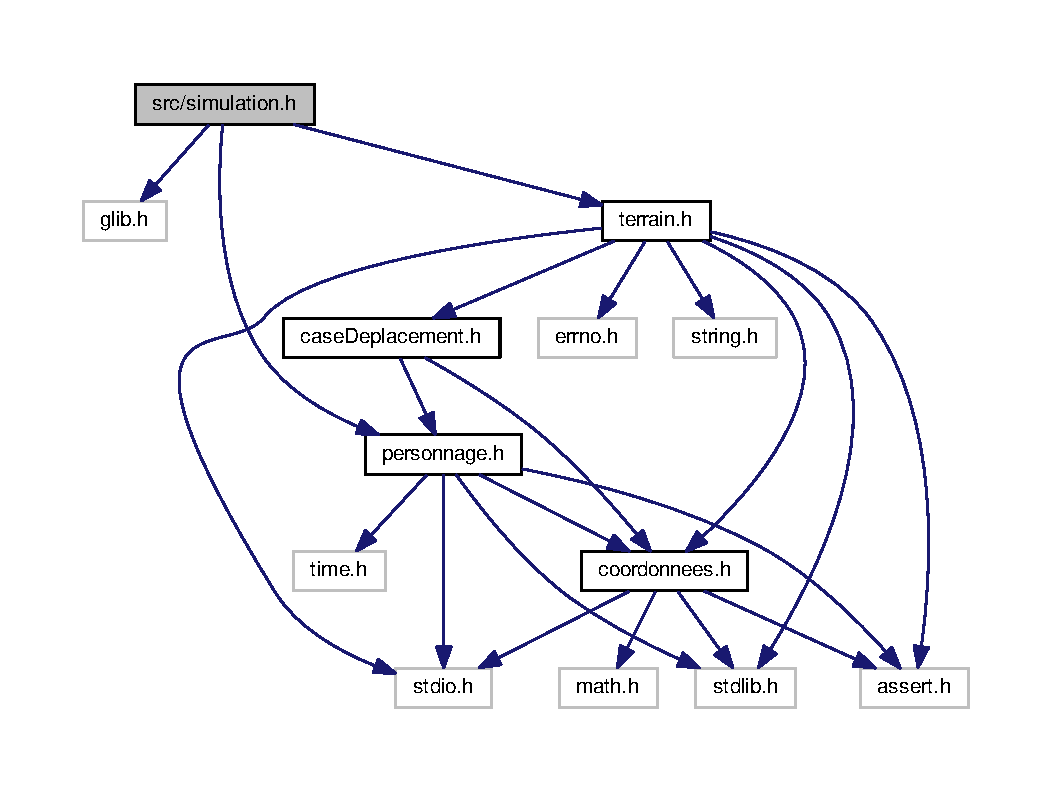
\includegraphics[width=350pt]{simulation_8h__incl}
\end{center}
\end{figure}
Ce graphe montre quels fichiers incluent directement ou indirectement ce fichier \+:
\nopagebreak
\begin{figure}[H]
\begin{center}
\leavevmode
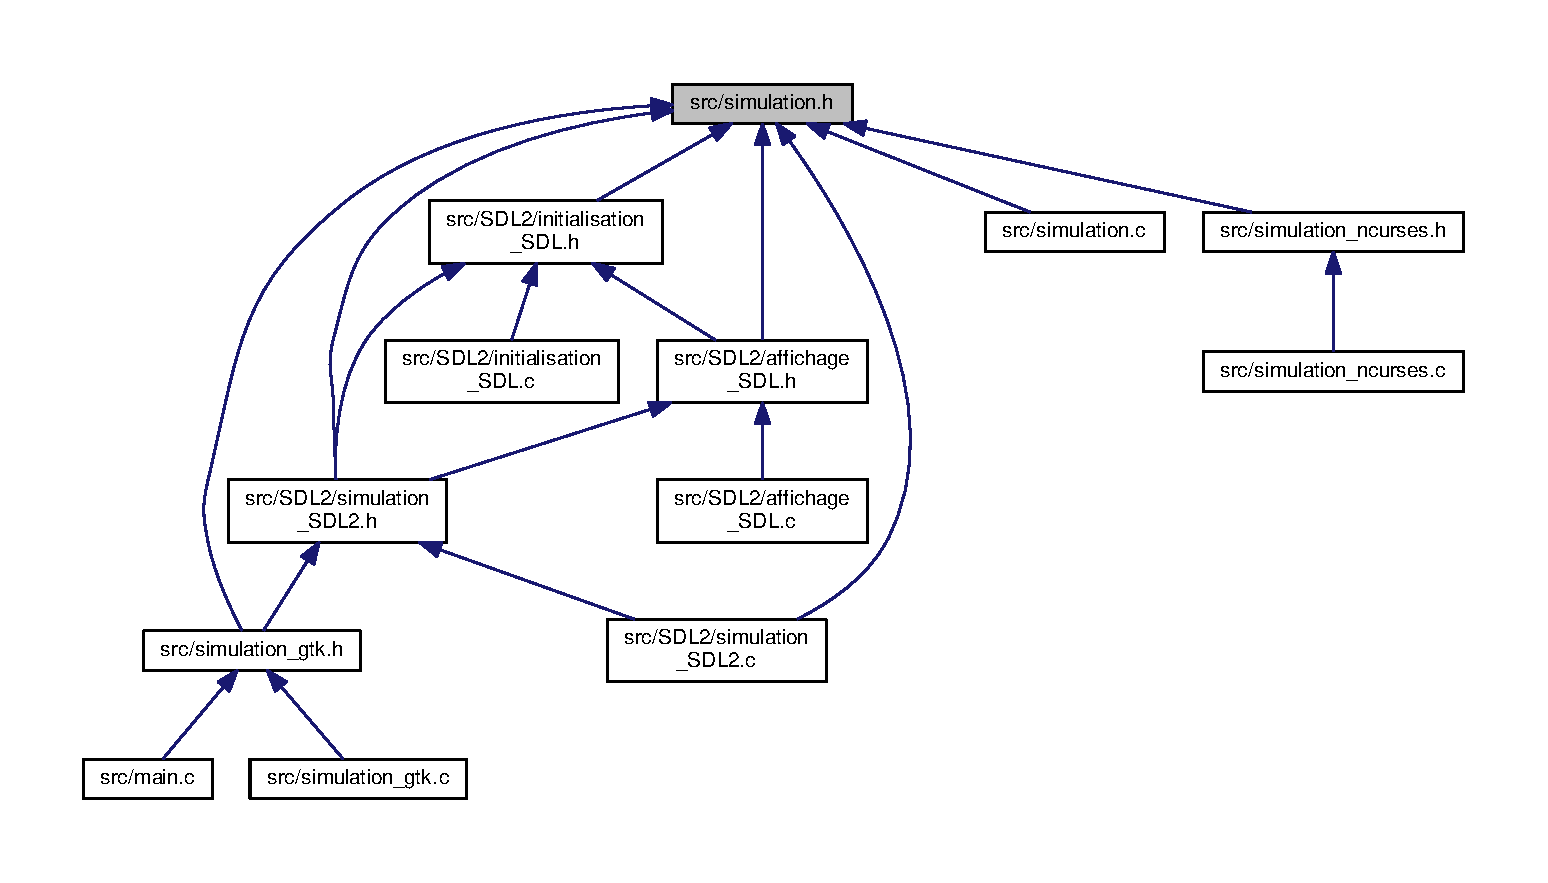
\includegraphics[width=350pt]{simulation_8h__dep__incl}
\end{center}
\end{figure}
\subsection*{Classes}
\begin{DoxyCompactItemize}
\item 
struct \hyperlink{structMSimulation}{M\+Simulation}
\begin{DoxyCompactList}\small\item\em Structure definissant une simulation et ses attributs. \end{DoxyCompactList}\end{DoxyCompactItemize}
\subsection*{Définitions de type}
\begin{DoxyCompactItemize}
\item 
typedef struct \hyperlink{structMSimulation}{M\+Simulation} \hyperlink{simulation_8h_a1ab3bf4791ab776bb4bd460dcce3e8d7}{Simulation}
\end{DoxyCompactItemize}
\subsection*{Fonctions}
\begin{DoxyCompactItemize}
\item 
\hyperlink{terrain_8h_a11bbfdc6f8212f3246205cc0e7134136}{Terrain} $\ast$ \hyperlink{simulation_8h_a7514376cebf0812d1c64d138766810d5}{get\+Terrain\+\_\+sim} (\hyperlink{simulation_8h_a1ab3bf4791ab776bb4bd460dcce3e8d7}{Simulation} $\ast$p\+Sim)
\begin{DoxyCompactList}\small\item\em Recupère le terrain associé à une Simulation. \end{DoxyCompactList}\item 
G\+Array $\ast$ \hyperlink{simulation_8h_aba7706e2cab7f8e20c98eaf6269fbdd8}{get\+Zombies\+\_\+sim} (\hyperlink{simulation_8h_a1ab3bf4791ab776bb4bd460dcce3e8d7}{Simulation} $\ast$p\+Sim)
\begin{DoxyCompactList}\small\item\em Recupère la grille de zombie associé à une Simulation. \end{DoxyCompactList}\item 
G\+Array $\ast$ \hyperlink{simulation_8h_a99b58cb2a89463b72b621aae2cc5c956}{get\+Citoyens\+\_\+sim} (\hyperlink{simulation_8h_a1ab3bf4791ab776bb4bd460dcce3e8d7}{Simulation} $\ast$p\+Sim)
\begin{DoxyCompactList}\small\item\em Recupère la grille de Citoyens associé à une Simulation. \end{DoxyCompactList}\item 
G\+Array $\ast$ \hyperlink{simulation_8h_a99c022a1fc4be8ea72049ed8548867cd}{get\+Policiers\+\_\+sim} (\hyperlink{simulation_8h_a1ab3bf4791ab776bb4bd460dcce3e8d7}{Simulation} $\ast$p\+Sim)
\begin{DoxyCompactList}\small\item\em Recupère la grille de Policiers associé à une Simulation. \end{DoxyCompactList}\item 
int \hyperlink{simulation_8h_a7c69cabd6bffbe631bd22d1d56e680a4}{get\+Nb\+Zombies\+\_\+sim} (\hyperlink{simulation_8h_a1ab3bf4791ab776bb4bd460dcce3e8d7}{Simulation} $\ast$p\+Sim)
\begin{DoxyCompactList}\small\item\em Recupère le nombre de zombie associé à une Simulation. \end{DoxyCompactList}\item 
int \hyperlink{simulation_8h_a9c811803ecb03ac907db8c2d5aa75c4a}{get\+Nb\+Citoyens\+\_\+sim} (\hyperlink{simulation_8h_a1ab3bf4791ab776bb4bd460dcce3e8d7}{Simulation} $\ast$p\+Sim)
\begin{DoxyCompactList}\small\item\em Recupère le nombre de Citoyens associé à une Simulation. \end{DoxyCompactList}\item 
int \hyperlink{simulation_8h_a71bd9dc4548a25fcaa7059e72e0850d2}{get\+Nb\+Policiers\+\_\+sim} (\hyperlink{simulation_8h_a1ab3bf4791ab776bb4bd460dcce3e8d7}{Simulation} $\ast$p\+Sim)
\begin{DoxyCompactList}\small\item\em Recupère le nombre de Policiers associé à une Simulation. \end{DoxyCompactList}\item 
void \hyperlink{simulation_8h_a44bfaa453f2d4a9cf897235adf4e0c9c}{zombies\+Init\+\_\+sim} (int nb\+Zombies, \hyperlink{simulation_8h_a1ab3bf4791ab776bb4bd460dcce3e8d7}{Simulation} $\ast$p\+Sim)
\begin{DoxyCompactList}\small\item\em Initialise la simulation avec un nombre de zombies. \end{DoxyCompactList}\item 
void \hyperlink{simulation_8h_aaa2bef8ef03449698a1c49f75e8f96bd}{citoyens\+Init\+\_\+sim} (int nb\+Citoyens, \hyperlink{simulation_8h_a1ab3bf4791ab776bb4bd460dcce3e8d7}{Simulation} $\ast$p\+Sim)
\begin{DoxyCompactList}\small\item\em Initialise la simulation avec un nombre de Citoyens. \end{DoxyCompactList}\item 
void \hyperlink{simulation_8h_a846fbbc98362da744d48198158e2d347}{policiers\+Init\+\_\+sim} (int nb\+Policiers, \hyperlink{simulation_8h_a1ab3bf4791ab776bb4bd460dcce3e8d7}{Simulation} $\ast$p\+Sim)
\begin{DoxyCompactList}\small\item\em Initialise la simulation avec un nombre de Policier. \end{DoxyCompactList}\item 
void \hyperlink{simulation_8h_a4099b743564c53f0a937d6d78c48e6e7}{terrain\+Init\+\_\+sim} (char $\ast$nom\+Fic, \hyperlink{simulation_8h_a1ab3bf4791ab776bb4bd460dcce3e8d7}{Simulation} $\ast$p\+Sim)
\begin{DoxyCompactList}\small\item\em Initialise la simulation avec le fichier de nom spécifié \end{DoxyCompactList}\item 
void \hyperlink{simulation_8h_a14f3cc9f6446c3f212a49d054d358394}{init\+Simulation\+\_\+sim} (\hyperlink{simulation_8h_a1ab3bf4791ab776bb4bd460dcce3e8d7}{Simulation} $\ast$p\+Sim, int nb\+Zombies, int nb\+Citoyens, int nb\+Policiers, char $\ast$nom\+Fic)
\begin{DoxyCompactList}\small\item\em Initialise la simulation avec le fichier de nom spécifié, le nombre de zombies, de citoyens et de policier, en appelant les fonctions spécifiques. \end{DoxyCompactList}\item 
\hyperlink{simulation_8h_a1ab3bf4791ab776bb4bd460dcce3e8d7}{Simulation} $\ast$ \hyperlink{simulation_8h_a66f239a8233da55d5a38fba5853809f5}{creer\+Simulation\+\_\+sim} (int nb\+Zombies, int nb\+Citoyens, int nb\+Policiers, char $\ast$nom\+Fic)
\begin{DoxyCompactList}\small\item\em Creer la simulation avec le fichier de nom spécifié, le nombre de zombies, de citoyens et de policier, en appelant les fonctions spécifiques, et l\textquotesingle{}initialise. \end{DoxyCompactList}\item 
void \hyperlink{simulation_8h_af61e27b9f0b0a9c55a56f3af37f90f74}{deplacer\+Policiers\+\_\+sim} (\hyperlink{simulation_8h_a1ab3bf4791ab776bb4bd460dcce3e8d7}{Simulation} $\ast$p\+Sim)
\begin{DoxyCompactList}\small\item\em Executes les deplacement des policiers de manière aléatoire. \end{DoxyCompactList}\item 
void \hyperlink{simulation_8h_a7be1f8001d8bc5edb63625a8fa8df70a}{deplacer\+Citoyens\+\_\+sim} (\hyperlink{simulation_8h_a1ab3bf4791ab776bb4bd460dcce3e8d7}{Simulation} $\ast$p\+Sim)
\begin{DoxyCompactList}\small\item\em Executes les deplacement des Citoyens de manière aléatoire. \end{DoxyCompactList}\item 
void \hyperlink{simulation_8h_a71d0dfc00495ee18d6a263e93a5cf8dd}{deplacer\+Zombies\+\_\+sim} (\hyperlink{simulation_8h_a1ab3bf4791ab776bb4bd460dcce3e8d7}{Simulation} $\ast$p\+Sim)
\begin{DoxyCompactList}\small\item\em Executes les deplacement des Zombies de manière aléatoire. \end{DoxyCompactList}\item 
void \hyperlink{simulation_8h_ad1f35ce5f9b80c161777a7e3b8cdee5a}{deplacer\+Perso\+\_\+sim} (\hyperlink{simulation_8h_a1ab3bf4791ab776bb4bd460dcce3e8d7}{Simulation} $\ast$p\+Sim)
\begin{DoxyCompactList}\small\item\em Executes les deplacement des personnages de manière aléatoire. \end{DoxyCompactList}\item 
void \hyperlink{simulation_8h_a99cf798b51aeb7a2828941fb096a9766}{deplacement\+Intel\+Zombies\+\_\+sim} (\hyperlink{simulation_8h_a1ab3bf4791ab776bb4bd460dcce3e8d7}{Simulation} $\ast$p\+Sim)
\begin{DoxyCompactList}\small\item\em Executes les deplacement des zombies de manière intelligente et en regard des champs. \end{DoxyCompactList}\item 
void \hyperlink{simulation_8h_acc4f40dd69c6516a19a38e065ee3395f}{deplacement\+Intel\+Citoyens\+\_\+sim} (\hyperlink{simulation_8h_a1ab3bf4791ab776bb4bd460dcce3e8d7}{Simulation} $\ast$p\+Sim)
\begin{DoxyCompactList}\small\item\em Executes les deplacement des Citoyens de manière intelligente et en regard des champs. \end{DoxyCompactList}\item 
void \hyperlink{simulation_8h_ab4c303981dc0289a2b211ba3e24ccf55}{deplacement\+Intel\+Policiers\+\_\+sim} (\hyperlink{simulation_8h_a1ab3bf4791ab776bb4bd460dcce3e8d7}{Simulation} $\ast$p\+Sim)
\begin{DoxyCompactList}\small\item\em Executes les deplacement des Policiers de manière intelligente et en regard des champs. \end{DoxyCompactList}\item 
void \hyperlink{simulation_8h_a1d3c4e9b6d1357086a629825e3d062cf}{deplacement\+Intel\+Persos} (\hyperlink{simulation_8h_a1ab3bf4791ab776bb4bd460dcce3e8d7}{Simulation} $\ast$p\+Sim)
\begin{DoxyCompactList}\small\item\em Executes les deplacement des personnages de manière intelligente et en regard des champs. \end{DoxyCompactList}\item 
void \hyperlink{simulation_8h_a4fc35a43279496971fef75d940492f7b}{ajouter\+Perso} (\hyperlink{coordonnees_8h_a79929cdfee7bd985a5e4e25276bb3ba9}{Coordonnees} $\ast$p\+Coord, enum \hyperlink{personnage_8h_a3f6a2951aa3d5d428dd6d61e74db0d75}{type\+Perso} type, \hyperlink{simulation_8h_a1ab3bf4791ab776bb4bd460dcce3e8d7}{Simulation} $\ast$p\+Sim)
\begin{DoxyCompactList}\small\item\em Ajoute un perso à la simulation et au terrain, selon son type. \end{DoxyCompactList}\item 
void \hyperlink{simulation_8h_a0ed5368338ff9e0871bb0c816135971a}{supprimer\+Perso} (\hyperlink{personnage_8h_abd5c92a453bbf273f753b3f5b99da9e7}{Perso} $\ast$p\+Perso, \hyperlink{simulation_8h_a1ab3bf4791ab776bb4bd460dcce3e8d7}{Simulation} $\ast$p\+Sim)
\begin{DoxyCompactList}\small\item\em Supprime un perso de la simulation et de la case à laquelle il est affecté. Ne libère les coordonnées affectées. \end{DoxyCompactList}\item 
void \hyperlink{simulation_8h_a8e9f7110fca5097ac2e3b0c5b37549af}{contaminations} (\hyperlink{simulation_8h_a1ab3bf4791ab776bb4bd460dcce3e8d7}{Simulation} $\ast$p\+Sim)
\begin{DoxyCompactList}\small\item\em Executes les instruction de contamination des policier et citoyens par les zombies. \end{DoxyCompactList}\item 
void \hyperlink{simulation_8h_abf7873243ac6158bd5dfac2dc3b376b1}{tirs} (\hyperlink{simulation_8h_a1ab3bf4791ab776bb4bd460dcce3e8d7}{Simulation} $\ast$p\+Sim)
\begin{DoxyCompactList}\small\item\em Executes les instruction de tirs des policiers sur les zombies. \end{DoxyCompactList}\item 
void \hyperlink{simulation_8h_aec9f9a901b4ea316a48612d15e772dfc}{propager\+Champs\+Persos} (\hyperlink{simulation_8h_a1ab3bf4791ab776bb4bd460dcce3e8d7}{Simulation} $\ast$p\+Sim)
\begin{DoxyCompactList}\small\item\em Propage les champs des personnages dans la simulation. \end{DoxyCompactList}\item 
void \hyperlink{simulation_8h_ac61d3c90dafcff499c3ec3d8095c88bb}{deplacement\+Intel\+Zombie} (\hyperlink{personnage_8h_abd5c92a453bbf273f753b3f5b99da9e7}{Perso} $\ast$p\+Perso, \hyperlink{simulation_8h_a1ab3bf4791ab776bb4bd460dcce3e8d7}{Simulation} $\ast$p\+Sim)
\begin{DoxyCompactList}\small\item\em Executes les instruction de deplacement intteligent d\textquotesingle{}un Zombie. \end{DoxyCompactList}\item 
void \hyperlink{simulation_8h_a119206545d9d380e685a18c9987d3856}{deplacement\+Intel\+Citoyen} (\hyperlink{personnage_8h_abd5c92a453bbf273f753b3f5b99da9e7}{Perso} $\ast$p\+Perso, \hyperlink{simulation_8h_a1ab3bf4791ab776bb4bd460dcce3e8d7}{Simulation} $\ast$p\+Sim)
\begin{DoxyCompactList}\small\item\em Executes les instruction de deplacement intteligent d\textquotesingle{}un Citoyen. \end{DoxyCompactList}\item 
void \hyperlink{simulation_8h_abd1af38115336e38d41f0c42123a2024}{deplacement\+Intel\+Policier} (\hyperlink{personnage_8h_abd5c92a453bbf273f753b3f5b99da9e7}{Perso} $\ast$p\+Perso, \hyperlink{simulation_8h_a1ab3bf4791ab776bb4bd460dcce3e8d7}{Simulation} $\ast$p\+Sim)
\begin{DoxyCompactList}\small\item\em Executes les instruction de deplacement intteligent d\textquotesingle{}un Policier. \end{DoxyCompactList}\item 
void \hyperlink{simulation_8h_a8c84b81dbfbacce2c792705198ee9f71}{test\+Fonctions\+\_\+sim} ()
\begin{DoxyCompactList}\small\item\em Focntions de test des fonctions du module Simulation. \end{DoxyCompactList}\item 
int \hyperlink{simulation_8h_a14a4e9bf4982b1fdd2b26a6f82d24fc0}{compare\+Tab2D} (const void $\ast$a, const void $\ast$b)
\begin{DoxyCompactList}\small\item\em Fonction à appeler avec qsort pour trier un tableau 2D en lignes par rapport à la première case. \end{DoxyCompactList}\end{DoxyCompactItemize}


\subsection{Description détaillée}
Définit la simulation, ses parametres et ses accesseurs. 



\subsection{Documentation des définitions de type}
\index{simulation.\+h@{simulation.\+h}!Simulation@{Simulation}}
\index{Simulation@{Simulation}!simulation.\+h@{simulation.\+h}}
\subsubsection[{\texorpdfstring{Simulation}{Simulation}}]{\setlength{\rightskip}{0pt plus 5cm}typedef struct {\bf M\+Simulation}  {\bf Simulation}}\hypertarget{simulation_8h_a1ab3bf4791ab776bb4bd460dcce3e8d7}{}\label{simulation_8h_a1ab3bf4791ab776bb4bd460dcce3e8d7}


\subsection{Documentation des fonctions}
\index{simulation.\+h@{simulation.\+h}!ajouter\+Perso@{ajouter\+Perso}}
\index{ajouter\+Perso@{ajouter\+Perso}!simulation.\+h@{simulation.\+h}}
\subsubsection[{\texorpdfstring{ajouter\+Perso(\+Coordonnees $\ast$p\+Coord, enum type\+Perso type, Simulation $\ast$p\+Sim)}{ajouterPerso(Coordonnees *pCoord, enum typePerso type, Simulation *pSim)}}]{\setlength{\rightskip}{0pt plus 5cm}void ajouter\+Perso (
\begin{DoxyParamCaption}
\item[{{\bf Coordonnees} $\ast$}]{p\+Coord, }
\item[{enum {\bf type\+Perso}}]{type, }
\item[{{\bf Simulation} $\ast$}]{p\+Sim}
\end{DoxyParamCaption}
)}\hypertarget{simulation_8h_a4fc35a43279496971fef75d940492f7b}{}\label{simulation_8h_a4fc35a43279496971fef75d940492f7b}


Ajoute un perso à la simulation et au terrain, selon son type. 


\begin{DoxyParams}{Paramètres}
{\em p\+Coord} & Coordonnées du personnage sur le terrain \\
\hline
{\em type} & Type du perso (Z\+O\+M\+B\+IE, P\+O\+L\+I\+C\+I\+ER, C\+I\+T\+O\+Y\+EN) \\
\hline
{\em p\+Sim} & Pointeur sur la simulation \\
\hline
\end{DoxyParams}
\index{simulation.\+h@{simulation.\+h}!citoyens\+Init\+\_\+sim@{citoyens\+Init\+\_\+sim}}
\index{citoyens\+Init\+\_\+sim@{citoyens\+Init\+\_\+sim}!simulation.\+h@{simulation.\+h}}
\subsubsection[{\texorpdfstring{citoyens\+Init\+\_\+sim(int nb\+Citoyens, Simulation $\ast$p\+Sim)}{citoyensInit_sim(int nbCitoyens, Simulation *pSim)}}]{\setlength{\rightskip}{0pt plus 5cm}void citoyens\+Init\+\_\+sim (
\begin{DoxyParamCaption}
\item[{int}]{nb\+Citoyens, }
\item[{{\bf Simulation} $\ast$}]{p\+Sim}
\end{DoxyParamCaption}
)}\hypertarget{simulation_8h_aaa2bef8ef03449698a1c49f75e8f96bd}{}\label{simulation_8h_aaa2bef8ef03449698a1c49f75e8f96bd}


Initialise la simulation avec un nombre de Citoyens. 


\begin{DoxyParams}{Paramètres}
{\em nb\+Citoyens} & Nombres de Citoyens a initialiser dans la Simulation \\
\hline
{\em p\+Sim} & La simulation a initialiser \\
\hline
\end{DoxyParams}
\index{simulation.\+h@{simulation.\+h}!compare\+Tab2D@{compare\+Tab2D}}
\index{compare\+Tab2D@{compare\+Tab2D}!simulation.\+h@{simulation.\+h}}
\subsubsection[{\texorpdfstring{compare\+Tab2\+D(const void $\ast$a, const void $\ast$b)}{compareTab2D(const void *a, const void *b)}}]{\setlength{\rightskip}{0pt plus 5cm}int compare\+Tab2D (
\begin{DoxyParamCaption}
\item[{const void $\ast$}]{a, }
\item[{const void $\ast$}]{b}
\end{DoxyParamCaption}
)}\hypertarget{simulation_8h_a14a4e9bf4982b1fdd2b26a6f82d24fc0}{}\label{simulation_8h_a14a4e9bf4982b1fdd2b26a6f82d24fc0}


Fonction à appeler avec qsort pour trier un tableau 2D en lignes par rapport à la première case. 


\begin{DoxyParams}{Paramètres}
{\em a} & Pointeur sur une case du tableau \\
\hline
{\em b} & Pointeur sur une case du tableau \\
\hline
\end{DoxyParams}
\index{simulation.\+h@{simulation.\+h}!contaminations@{contaminations}}
\index{contaminations@{contaminations}!simulation.\+h@{simulation.\+h}}
\subsubsection[{\texorpdfstring{contaminations(\+Simulation $\ast$p\+Sim)}{contaminations(Simulation *pSim)}}]{\setlength{\rightskip}{0pt plus 5cm}void contaminations (
\begin{DoxyParamCaption}
\item[{{\bf Simulation} $\ast$}]{p\+Sim}
\end{DoxyParamCaption}
)}\hypertarget{simulation_8h_a8e9f7110fca5097ac2e3b0c5b37549af}{}\label{simulation_8h_a8e9f7110fca5097ac2e3b0c5b37549af}


Executes les instruction de contamination des policier et citoyens par les zombies. 


\begin{DoxyParams}{Paramètres}
{\em p\+Sim} & La simulation dans laquelle tout est effectué \\
\hline
\end{DoxyParams}
\index{simulation.\+h@{simulation.\+h}!creer\+Simulation\+\_\+sim@{creer\+Simulation\+\_\+sim}}
\index{creer\+Simulation\+\_\+sim@{creer\+Simulation\+\_\+sim}!simulation.\+h@{simulation.\+h}}
\subsubsection[{\texorpdfstring{creer\+Simulation\+\_\+sim(int nb\+Zombies, int nb\+Citoyens, int nb\+Policiers, char $\ast$nom\+Fic)}{creerSimulation_sim(int nbZombies, int nbCitoyens, int nbPoliciers, char *nomFic)}}]{\setlength{\rightskip}{0pt plus 5cm}{\bf Simulation}$\ast$ creer\+Simulation\+\_\+sim (
\begin{DoxyParamCaption}
\item[{int}]{nb\+Zombies, }
\item[{int}]{nb\+Citoyens, }
\item[{int}]{nb\+Policiers, }
\item[{char $\ast$}]{nom\+Fic}
\end{DoxyParamCaption}
)}\hypertarget{simulation_8h_a66f239a8233da55d5a38fba5853809f5}{}\label{simulation_8h_a66f239a8233da55d5a38fba5853809f5}


Creer la simulation avec le fichier de nom spécifié, le nombre de zombies, de citoyens et de policier, en appelant les fonctions spécifiques, et l\textquotesingle{}initialise. 


\begin{DoxyParams}{Paramètres}
{\em nb\+Zombies} & Nombres de zombies a creer dans la Simulation \\
\hline
{\em nb\+Citoyens} & Nombres de Citoyens a creer dans la Simulation \\
\hline
{\em nb\+Policiers} & Nombres de Policiers a creer dans la Simulation \\
\hline
{\em nom\+Fic} & Chaine de caractère de nom du fichier \\
\hline
\end{DoxyParams}
\begin{DoxyReturn}{Renvoie}
p\+Sim Pointeur vers la Simulation crée 
\end{DoxyReturn}
\index{simulation.\+h@{simulation.\+h}!deplacement\+Intel\+Citoyen@{deplacement\+Intel\+Citoyen}}
\index{deplacement\+Intel\+Citoyen@{deplacement\+Intel\+Citoyen}!simulation.\+h@{simulation.\+h}}
\subsubsection[{\texorpdfstring{deplacement\+Intel\+Citoyen(\+Perso $\ast$p\+Perso, Simulation $\ast$p\+Sim)}{deplacementIntelCitoyen(Perso *pPerso, Simulation *pSim)}}]{\setlength{\rightskip}{0pt plus 5cm}void deplacement\+Intel\+Citoyen (
\begin{DoxyParamCaption}
\item[{{\bf Perso} $\ast$}]{p\+Perso, }
\item[{{\bf Simulation} $\ast$}]{p\+Sim}
\end{DoxyParamCaption}
)}\hypertarget{simulation_8h_a119206545d9d380e685a18c9987d3856}{}\label{simulation_8h_a119206545d9d380e685a18c9987d3856}


Executes les instruction de deplacement intteligent d\textquotesingle{}un Citoyen. 


\begin{DoxyParams}{Paramètres}
{\em p\+Perso} & Pointeur vers l\textquotesingle{}entité qui va etre déplacé intelligement \\
\hline
{\em p\+Sim} & La simulation dans laquelle tout est effectué \\
\hline
\end{DoxyParams}
\index{simulation.\+h@{simulation.\+h}!deplacement\+Intel\+Citoyens\+\_\+sim@{deplacement\+Intel\+Citoyens\+\_\+sim}}
\index{deplacement\+Intel\+Citoyens\+\_\+sim@{deplacement\+Intel\+Citoyens\+\_\+sim}!simulation.\+h@{simulation.\+h}}
\subsubsection[{\texorpdfstring{deplacement\+Intel\+Citoyens\+\_\+sim(\+Simulation $\ast$p\+Sim)}{deplacementIntelCitoyens_sim(Simulation *pSim)}}]{\setlength{\rightskip}{0pt plus 5cm}void deplacement\+Intel\+Citoyens\+\_\+sim (
\begin{DoxyParamCaption}
\item[{{\bf Simulation} $\ast$}]{p\+Sim}
\end{DoxyParamCaption}
)}\hypertarget{simulation_8h_acc4f40dd69c6516a19a38e065ee3395f}{}\label{simulation_8h_acc4f40dd69c6516a19a38e065ee3395f}


Executes les deplacement des Citoyens de manière intelligente et en regard des champs. 


\begin{DoxyParams}{Paramètres}
{\em p\+Sim} & La simulation dans laquelle tout est effectué \\
\hline
\end{DoxyParams}
\index{simulation.\+h@{simulation.\+h}!deplacement\+Intel\+Persos@{deplacement\+Intel\+Persos}}
\index{deplacement\+Intel\+Persos@{deplacement\+Intel\+Persos}!simulation.\+h@{simulation.\+h}}
\subsubsection[{\texorpdfstring{deplacement\+Intel\+Persos(\+Simulation $\ast$p\+Sim)}{deplacementIntelPersos(Simulation *pSim)}}]{\setlength{\rightskip}{0pt plus 5cm}void deplacement\+Intel\+Persos (
\begin{DoxyParamCaption}
\item[{{\bf Simulation} $\ast$}]{p\+Sim}
\end{DoxyParamCaption}
)}\hypertarget{simulation_8h_a1d3c4e9b6d1357086a629825e3d062cf}{}\label{simulation_8h_a1d3c4e9b6d1357086a629825e3d062cf}


Executes les deplacement des personnages de manière intelligente et en regard des champs. 


\begin{DoxyParams}{Paramètres}
{\em p\+Sim} & La simulation dans laquelle tout est effectué \\
\hline
\end{DoxyParams}
\index{simulation.\+h@{simulation.\+h}!deplacement\+Intel\+Policier@{deplacement\+Intel\+Policier}}
\index{deplacement\+Intel\+Policier@{deplacement\+Intel\+Policier}!simulation.\+h@{simulation.\+h}}
\subsubsection[{\texorpdfstring{deplacement\+Intel\+Policier(\+Perso $\ast$p\+Perso, Simulation $\ast$p\+Sim)}{deplacementIntelPolicier(Perso *pPerso, Simulation *pSim)}}]{\setlength{\rightskip}{0pt plus 5cm}void deplacement\+Intel\+Policier (
\begin{DoxyParamCaption}
\item[{{\bf Perso} $\ast$}]{p\+Perso, }
\item[{{\bf Simulation} $\ast$}]{p\+Sim}
\end{DoxyParamCaption}
)}\hypertarget{simulation_8h_abd1af38115336e38d41f0c42123a2024}{}\label{simulation_8h_abd1af38115336e38d41f0c42123a2024}


Executes les instruction de deplacement intteligent d\textquotesingle{}un Policier. 


\begin{DoxyParams}{Paramètres}
{\em p\+Perso} & Pointeur vers l\textquotesingle{}entité qui va etre déplacé intelligement \\
\hline
{\em p\+Sim} & La simulation dans laquelle tout est effectué \\
\hline
\end{DoxyParams}
\index{simulation.\+h@{simulation.\+h}!deplacement\+Intel\+Policiers\+\_\+sim@{deplacement\+Intel\+Policiers\+\_\+sim}}
\index{deplacement\+Intel\+Policiers\+\_\+sim@{deplacement\+Intel\+Policiers\+\_\+sim}!simulation.\+h@{simulation.\+h}}
\subsubsection[{\texorpdfstring{deplacement\+Intel\+Policiers\+\_\+sim(\+Simulation $\ast$p\+Sim)}{deplacementIntelPoliciers_sim(Simulation *pSim)}}]{\setlength{\rightskip}{0pt plus 5cm}void deplacement\+Intel\+Policiers\+\_\+sim (
\begin{DoxyParamCaption}
\item[{{\bf Simulation} $\ast$}]{p\+Sim}
\end{DoxyParamCaption}
)}\hypertarget{simulation_8h_ab4c303981dc0289a2b211ba3e24ccf55}{}\label{simulation_8h_ab4c303981dc0289a2b211ba3e24ccf55}


Executes les deplacement des Policiers de manière intelligente et en regard des champs. 


\begin{DoxyParams}{Paramètres}
{\em p\+Sim} & La simulation dans laquelle tout est effectué \\
\hline
\end{DoxyParams}
\index{simulation.\+h@{simulation.\+h}!deplacement\+Intel\+Zombie@{deplacement\+Intel\+Zombie}}
\index{deplacement\+Intel\+Zombie@{deplacement\+Intel\+Zombie}!simulation.\+h@{simulation.\+h}}
\subsubsection[{\texorpdfstring{deplacement\+Intel\+Zombie(\+Perso $\ast$p\+Perso, Simulation $\ast$p\+Sim)}{deplacementIntelZombie(Perso *pPerso, Simulation *pSim)}}]{\setlength{\rightskip}{0pt plus 5cm}void deplacement\+Intel\+Zombie (
\begin{DoxyParamCaption}
\item[{{\bf Perso} $\ast$}]{p\+Perso, }
\item[{{\bf Simulation} $\ast$}]{p\+Sim}
\end{DoxyParamCaption}
)}\hypertarget{simulation_8h_ac61d3c90dafcff499c3ec3d8095c88bb}{}\label{simulation_8h_ac61d3c90dafcff499c3ec3d8095c88bb}


Executes les instruction de deplacement intteligent d\textquotesingle{}un Zombie. 


\begin{DoxyParams}{Paramètres}
{\em p\+Perso} & Pointeur vers l\textquotesingle{}entité qui va etre déplacé intelligement \\
\hline
{\em p\+Sim} & La simulation dans laquelle tout est effectué \\
\hline
\end{DoxyParams}
\index{simulation.\+h@{simulation.\+h}!deplacement\+Intel\+Zombies\+\_\+sim@{deplacement\+Intel\+Zombies\+\_\+sim}}
\index{deplacement\+Intel\+Zombies\+\_\+sim@{deplacement\+Intel\+Zombies\+\_\+sim}!simulation.\+h@{simulation.\+h}}
\subsubsection[{\texorpdfstring{deplacement\+Intel\+Zombies\+\_\+sim(\+Simulation $\ast$p\+Sim)}{deplacementIntelZombies_sim(Simulation *pSim)}}]{\setlength{\rightskip}{0pt plus 5cm}void deplacement\+Intel\+Zombies\+\_\+sim (
\begin{DoxyParamCaption}
\item[{{\bf Simulation} $\ast$}]{p\+Sim}
\end{DoxyParamCaption}
)}\hypertarget{simulation_8h_a99cf798b51aeb7a2828941fb096a9766}{}\label{simulation_8h_a99cf798b51aeb7a2828941fb096a9766}


Executes les deplacement des zombies de manière intelligente et en regard des champs. 


\begin{DoxyParams}{Paramètres}
{\em p\+Sim} & La simulation dans laquelle tout est effectué \\
\hline
\end{DoxyParams}
\index{simulation.\+h@{simulation.\+h}!deplacer\+Citoyens\+\_\+sim@{deplacer\+Citoyens\+\_\+sim}}
\index{deplacer\+Citoyens\+\_\+sim@{deplacer\+Citoyens\+\_\+sim}!simulation.\+h@{simulation.\+h}}
\subsubsection[{\texorpdfstring{deplacer\+Citoyens\+\_\+sim(\+Simulation $\ast$p\+Sim)}{deplacerCitoyens_sim(Simulation *pSim)}}]{\setlength{\rightskip}{0pt plus 5cm}void deplacer\+Citoyens\+\_\+sim (
\begin{DoxyParamCaption}
\item[{{\bf Simulation} $\ast$}]{p\+Sim}
\end{DoxyParamCaption}
)}\hypertarget{simulation_8h_a7be1f8001d8bc5edb63625a8fa8df70a}{}\label{simulation_8h_a7be1f8001d8bc5edb63625a8fa8df70a}


Executes les deplacement des Citoyens de manière aléatoire. 


\begin{DoxyParams}{Paramètres}
{\em p\+Sim} & La simulation dans laquelle tout est effectué \\
\hline
\end{DoxyParams}
\index{simulation.\+h@{simulation.\+h}!deplacer\+Perso\+\_\+sim@{deplacer\+Perso\+\_\+sim}}
\index{deplacer\+Perso\+\_\+sim@{deplacer\+Perso\+\_\+sim}!simulation.\+h@{simulation.\+h}}
\subsubsection[{\texorpdfstring{deplacer\+Perso\+\_\+sim(\+Simulation $\ast$p\+Sim)}{deplacerPerso_sim(Simulation *pSim)}}]{\setlength{\rightskip}{0pt plus 5cm}void deplacer\+Perso\+\_\+sim (
\begin{DoxyParamCaption}
\item[{{\bf Simulation} $\ast$}]{p\+Sim}
\end{DoxyParamCaption}
)}\hypertarget{simulation_8h_ad1f35ce5f9b80c161777a7e3b8cdee5a}{}\label{simulation_8h_ad1f35ce5f9b80c161777a7e3b8cdee5a}


Executes les deplacement des personnages de manière aléatoire. 


\begin{DoxyParams}{Paramètres}
{\em p\+Sim} & La simulation dans laquelle tout est effectué \\
\hline
\end{DoxyParams}
\index{simulation.\+h@{simulation.\+h}!deplacer\+Policiers\+\_\+sim@{deplacer\+Policiers\+\_\+sim}}
\index{deplacer\+Policiers\+\_\+sim@{deplacer\+Policiers\+\_\+sim}!simulation.\+h@{simulation.\+h}}
\subsubsection[{\texorpdfstring{deplacer\+Policiers\+\_\+sim(\+Simulation $\ast$p\+Sim)}{deplacerPoliciers_sim(Simulation *pSim)}}]{\setlength{\rightskip}{0pt plus 5cm}void deplacer\+Policiers\+\_\+sim (
\begin{DoxyParamCaption}
\item[{{\bf Simulation} $\ast$}]{p\+Sim}
\end{DoxyParamCaption}
)}\hypertarget{simulation_8h_af61e27b9f0b0a9c55a56f3af37f90f74}{}\label{simulation_8h_af61e27b9f0b0a9c55a56f3af37f90f74}


Executes les deplacement des policiers de manière aléatoire. 


\begin{DoxyParams}{Paramètres}
{\em p\+Sim} & La simulation dans laquelle tout est effectué \\
\hline
\end{DoxyParams}
\index{simulation.\+h@{simulation.\+h}!deplacer\+Zombies\+\_\+sim@{deplacer\+Zombies\+\_\+sim}}
\index{deplacer\+Zombies\+\_\+sim@{deplacer\+Zombies\+\_\+sim}!simulation.\+h@{simulation.\+h}}
\subsubsection[{\texorpdfstring{deplacer\+Zombies\+\_\+sim(\+Simulation $\ast$p\+Sim)}{deplacerZombies_sim(Simulation *pSim)}}]{\setlength{\rightskip}{0pt plus 5cm}void deplacer\+Zombies\+\_\+sim (
\begin{DoxyParamCaption}
\item[{{\bf Simulation} $\ast$}]{p\+Sim}
\end{DoxyParamCaption}
)}\hypertarget{simulation_8h_a71d0dfc00495ee18d6a263e93a5cf8dd}{}\label{simulation_8h_a71d0dfc00495ee18d6a263e93a5cf8dd}


Executes les deplacement des Zombies de manière aléatoire. 


\begin{DoxyParams}{Paramètres}
{\em p\+Sim} & La simulation dans laquelle tout est effectué \\
\hline
\end{DoxyParams}
\index{simulation.\+h@{simulation.\+h}!get\+Citoyens\+\_\+sim@{get\+Citoyens\+\_\+sim}}
\index{get\+Citoyens\+\_\+sim@{get\+Citoyens\+\_\+sim}!simulation.\+h@{simulation.\+h}}
\subsubsection[{\texorpdfstring{get\+Citoyens\+\_\+sim(\+Simulation $\ast$p\+Sim)}{getCitoyens_sim(Simulation *pSim)}}]{\setlength{\rightskip}{0pt plus 5cm}G\+Array$\ast$ get\+Citoyens\+\_\+sim (
\begin{DoxyParamCaption}
\item[{{\bf Simulation} $\ast$}]{p\+Sim}
\end{DoxyParamCaption}
)}\hypertarget{simulation_8h_a99b58cb2a89463b72b621aae2cc5c956}{}\label{simulation_8h_a99b58cb2a89463b72b621aae2cc5c956}


Recupère la grille de Citoyens associé à une Simulation. 


\begin{DoxyParams}{Paramètres}
{\em p\+Sim} & La simulation a étudier \\
\hline
\end{DoxyParams}
\begin{DoxyReturn}{Renvoie}
Pointeur vers la grille de Citoyens 
\end{DoxyReturn}
\index{simulation.\+h@{simulation.\+h}!get\+Nb\+Citoyens\+\_\+sim@{get\+Nb\+Citoyens\+\_\+sim}}
\index{get\+Nb\+Citoyens\+\_\+sim@{get\+Nb\+Citoyens\+\_\+sim}!simulation.\+h@{simulation.\+h}}
\subsubsection[{\texorpdfstring{get\+Nb\+Citoyens\+\_\+sim(\+Simulation $\ast$p\+Sim)}{getNbCitoyens_sim(Simulation *pSim)}}]{\setlength{\rightskip}{0pt plus 5cm}int get\+Nb\+Citoyens\+\_\+sim (
\begin{DoxyParamCaption}
\item[{{\bf Simulation} $\ast$}]{p\+Sim}
\end{DoxyParamCaption}
)}\hypertarget{simulation_8h_a9c811803ecb03ac907db8c2d5aa75c4a}{}\label{simulation_8h_a9c811803ecb03ac907db8c2d5aa75c4a}


Recupère le nombre de Citoyens associé à une Simulation. 


\begin{DoxyParams}{Paramètres}
{\em p\+Sim} & La simulation a étudier \\
\hline
\end{DoxyParams}
\begin{DoxyReturn}{Renvoie}
Entier du nombre de Citoyens dans la Simulation 
\end{DoxyReturn}
\index{simulation.\+h@{simulation.\+h}!get\+Nb\+Policiers\+\_\+sim@{get\+Nb\+Policiers\+\_\+sim}}
\index{get\+Nb\+Policiers\+\_\+sim@{get\+Nb\+Policiers\+\_\+sim}!simulation.\+h@{simulation.\+h}}
\subsubsection[{\texorpdfstring{get\+Nb\+Policiers\+\_\+sim(\+Simulation $\ast$p\+Sim)}{getNbPoliciers_sim(Simulation *pSim)}}]{\setlength{\rightskip}{0pt plus 5cm}int get\+Nb\+Policiers\+\_\+sim (
\begin{DoxyParamCaption}
\item[{{\bf Simulation} $\ast$}]{p\+Sim}
\end{DoxyParamCaption}
)}\hypertarget{simulation_8h_a71bd9dc4548a25fcaa7059e72e0850d2}{}\label{simulation_8h_a71bd9dc4548a25fcaa7059e72e0850d2}


Recupère le nombre de Policiers associé à une Simulation. 


\begin{DoxyParams}{Paramètres}
{\em p\+Sim} & La simulation a étudier \\
\hline
\end{DoxyParams}
\begin{DoxyReturn}{Renvoie}
Entier du nombre de Policiers dans la Simulation 
\end{DoxyReturn}
\index{simulation.\+h@{simulation.\+h}!get\+Nb\+Zombies\+\_\+sim@{get\+Nb\+Zombies\+\_\+sim}}
\index{get\+Nb\+Zombies\+\_\+sim@{get\+Nb\+Zombies\+\_\+sim}!simulation.\+h@{simulation.\+h}}
\subsubsection[{\texorpdfstring{get\+Nb\+Zombies\+\_\+sim(\+Simulation $\ast$p\+Sim)}{getNbZombies_sim(Simulation *pSim)}}]{\setlength{\rightskip}{0pt plus 5cm}int get\+Nb\+Zombies\+\_\+sim (
\begin{DoxyParamCaption}
\item[{{\bf Simulation} $\ast$}]{p\+Sim}
\end{DoxyParamCaption}
)}\hypertarget{simulation_8h_a7c69cabd6bffbe631bd22d1d56e680a4}{}\label{simulation_8h_a7c69cabd6bffbe631bd22d1d56e680a4}


Recupère le nombre de zombie associé à une Simulation. 


\begin{DoxyParams}{Paramètres}
{\em p\+Sim} & La simulation a étudier \\
\hline
\end{DoxyParams}
\begin{DoxyReturn}{Renvoie}
Entier du nombre de zombie dans la Simulation 
\end{DoxyReturn}
\index{simulation.\+h@{simulation.\+h}!get\+Policiers\+\_\+sim@{get\+Policiers\+\_\+sim}}
\index{get\+Policiers\+\_\+sim@{get\+Policiers\+\_\+sim}!simulation.\+h@{simulation.\+h}}
\subsubsection[{\texorpdfstring{get\+Policiers\+\_\+sim(\+Simulation $\ast$p\+Sim)}{getPoliciers_sim(Simulation *pSim)}}]{\setlength{\rightskip}{0pt plus 5cm}G\+Array$\ast$ get\+Policiers\+\_\+sim (
\begin{DoxyParamCaption}
\item[{{\bf Simulation} $\ast$}]{p\+Sim}
\end{DoxyParamCaption}
)}\hypertarget{simulation_8h_a99c022a1fc4be8ea72049ed8548867cd}{}\label{simulation_8h_a99c022a1fc4be8ea72049ed8548867cd}


Recupère la grille de Policiers associé à une Simulation. 


\begin{DoxyParams}{Paramètres}
{\em p\+Sim} & La simulation a étudier \\
\hline
\end{DoxyParams}
\begin{DoxyReturn}{Renvoie}
Pointeur vers la grille de Policiers 
\end{DoxyReturn}
\index{simulation.\+h@{simulation.\+h}!get\+Terrain\+\_\+sim@{get\+Terrain\+\_\+sim}}
\index{get\+Terrain\+\_\+sim@{get\+Terrain\+\_\+sim}!simulation.\+h@{simulation.\+h}}
\subsubsection[{\texorpdfstring{get\+Terrain\+\_\+sim(\+Simulation $\ast$p\+Sim)}{getTerrain_sim(Simulation *pSim)}}]{\setlength{\rightskip}{0pt plus 5cm}{\bf Terrain}$\ast$ get\+Terrain\+\_\+sim (
\begin{DoxyParamCaption}
\item[{{\bf Simulation} $\ast$}]{p\+Sim}
\end{DoxyParamCaption}
)}\hypertarget{simulation_8h_a7514376cebf0812d1c64d138766810d5}{}\label{simulation_8h_a7514376cebf0812d1c64d138766810d5}


Recupère le terrain associé à une Simulation. 


\begin{DoxyParams}{Paramètres}
{\em p\+Sim} & La simulation a étudier \\
\hline
\end{DoxyParams}
\begin{DoxyReturn}{Renvoie}
Pointeur vers le terrain récupéré 
\end{DoxyReturn}
\index{simulation.\+h@{simulation.\+h}!get\+Zombies\+\_\+sim@{get\+Zombies\+\_\+sim}}
\index{get\+Zombies\+\_\+sim@{get\+Zombies\+\_\+sim}!simulation.\+h@{simulation.\+h}}
\subsubsection[{\texorpdfstring{get\+Zombies\+\_\+sim(\+Simulation $\ast$p\+Sim)}{getZombies_sim(Simulation *pSim)}}]{\setlength{\rightskip}{0pt plus 5cm}G\+Array$\ast$ get\+Zombies\+\_\+sim (
\begin{DoxyParamCaption}
\item[{{\bf Simulation} $\ast$}]{p\+Sim}
\end{DoxyParamCaption}
)}\hypertarget{simulation_8h_aba7706e2cab7f8e20c98eaf6269fbdd8}{}\label{simulation_8h_aba7706e2cab7f8e20c98eaf6269fbdd8}


Recupère la grille de zombie associé à une Simulation. 


\begin{DoxyParams}{Paramètres}
{\em p\+Sim} & La simulation a étudier \\
\hline
\end{DoxyParams}
\begin{DoxyReturn}{Renvoie}
Pointeur vers la grille de zombies 
\end{DoxyReturn}
\index{simulation.\+h@{simulation.\+h}!init\+Simulation\+\_\+sim@{init\+Simulation\+\_\+sim}}
\index{init\+Simulation\+\_\+sim@{init\+Simulation\+\_\+sim}!simulation.\+h@{simulation.\+h}}
\subsubsection[{\texorpdfstring{init\+Simulation\+\_\+sim(\+Simulation $\ast$p\+Sim, int nb\+Zombies, int nb\+Citoyens, int nb\+Policiers, char $\ast$nom\+Fic)}{initSimulation_sim(Simulation *pSim, int nbZombies, int nbCitoyens, int nbPoliciers, char *nomFic)}}]{\setlength{\rightskip}{0pt plus 5cm}void init\+Simulation\+\_\+sim (
\begin{DoxyParamCaption}
\item[{{\bf Simulation} $\ast$}]{p\+Sim, }
\item[{int}]{nb\+Zombies, }
\item[{int}]{nb\+Citoyens, }
\item[{int}]{nb\+Policiers, }
\item[{char $\ast$}]{nom\+Fic}
\end{DoxyParamCaption}
)}\hypertarget{simulation_8h_a14f3cc9f6446c3f212a49d054d358394}{}\label{simulation_8h_a14f3cc9f6446c3f212a49d054d358394}


Initialise la simulation avec le fichier de nom spécifié, le nombre de zombies, de citoyens et de policier, en appelant les fonctions spécifiques. 


\begin{DoxyParams}{Paramètres}
{\em p\+Sim} & La simulation a initialiser \\
\hline
{\em nb\+Zombies} & Nombres de zombies a initialiser dans la Simulation \\
\hline
{\em nb\+Citoyens} & Nombres de Citoyens a initialiser dans la Simulation \\
\hline
{\em nb\+Policiers} & Nombres de Policiers a initialiser dans la Simulation \\
\hline
{\em nom\+Fic} & Chaine de caractère de nom du fichier \\
\hline
\end{DoxyParams}
\index{simulation.\+h@{simulation.\+h}!policiers\+Init\+\_\+sim@{policiers\+Init\+\_\+sim}}
\index{policiers\+Init\+\_\+sim@{policiers\+Init\+\_\+sim}!simulation.\+h@{simulation.\+h}}
\subsubsection[{\texorpdfstring{policiers\+Init\+\_\+sim(int nb\+Policiers, Simulation $\ast$p\+Sim)}{policiersInit_sim(int nbPoliciers, Simulation *pSim)}}]{\setlength{\rightskip}{0pt plus 5cm}void policiers\+Init\+\_\+sim (
\begin{DoxyParamCaption}
\item[{int}]{nb\+Policiers, }
\item[{{\bf Simulation} $\ast$}]{p\+Sim}
\end{DoxyParamCaption}
)}\hypertarget{simulation_8h_a846fbbc98362da744d48198158e2d347}{}\label{simulation_8h_a846fbbc98362da744d48198158e2d347}


Initialise la simulation avec un nombre de Policier. 


\begin{DoxyParams}{Paramètres}
{\em nb\+Policiers} & Nombres de Policiers a initialiser dans la Simulation \\
\hline
{\em p\+Sim} & La simulation a initialiser \\
\hline
\end{DoxyParams}
\index{simulation.\+h@{simulation.\+h}!propager\+Champs\+Persos@{propager\+Champs\+Persos}}
\index{propager\+Champs\+Persos@{propager\+Champs\+Persos}!simulation.\+h@{simulation.\+h}}
\subsubsection[{\texorpdfstring{propager\+Champs\+Persos(\+Simulation $\ast$p\+Sim)}{propagerChampsPersos(Simulation *pSim)}}]{\setlength{\rightskip}{0pt plus 5cm}void propager\+Champs\+Persos (
\begin{DoxyParamCaption}
\item[{{\bf Simulation} $\ast$}]{p\+Sim}
\end{DoxyParamCaption}
)}\hypertarget{simulation_8h_aec9f9a901b4ea316a48612d15e772dfc}{}\label{simulation_8h_aec9f9a901b4ea316a48612d15e772dfc}


Propage les champs des personnages dans la simulation. 


\begin{DoxyParams}{Paramètres}
{\em p\+Sim} & La simulation dans laquelle tout est effectué \\
\hline
\end{DoxyParams}
\index{simulation.\+h@{simulation.\+h}!supprimer\+Perso@{supprimer\+Perso}}
\index{supprimer\+Perso@{supprimer\+Perso}!simulation.\+h@{simulation.\+h}}
\subsubsection[{\texorpdfstring{supprimer\+Perso(\+Perso $\ast$p\+Perso, Simulation $\ast$p\+Sim)}{supprimerPerso(Perso *pPerso, Simulation *pSim)}}]{\setlength{\rightskip}{0pt plus 5cm}void supprimer\+Perso (
\begin{DoxyParamCaption}
\item[{{\bf Perso} $\ast$}]{p\+Perso, }
\item[{{\bf Simulation} $\ast$}]{p\+Sim}
\end{DoxyParamCaption}
)}\hypertarget{simulation_8h_a0ed5368338ff9e0871bb0c816135971a}{}\label{simulation_8h_a0ed5368338ff9e0871bb0c816135971a}


Supprime un perso de la simulation et de la case à laquelle il est affecté. Ne libère les coordonnées affectées. 


\begin{DoxyParams}{Paramètres}
{\em p\+Perso} & Personnage à supprimer de la simulation \\
\hline
{\em p\+Sim} & La simulation dans laquelle tout est effectué \\
\hline
\end{DoxyParams}
\index{simulation.\+h@{simulation.\+h}!terrain\+Init\+\_\+sim@{terrain\+Init\+\_\+sim}}
\index{terrain\+Init\+\_\+sim@{terrain\+Init\+\_\+sim}!simulation.\+h@{simulation.\+h}}
\subsubsection[{\texorpdfstring{terrain\+Init\+\_\+sim(char $\ast$nom\+Fic, Simulation $\ast$p\+Sim)}{terrainInit_sim(char *nomFic, Simulation *pSim)}}]{\setlength{\rightskip}{0pt plus 5cm}void terrain\+Init\+\_\+sim (
\begin{DoxyParamCaption}
\item[{char $\ast$}]{nom\+Fic, }
\item[{{\bf Simulation} $\ast$}]{p\+Sim}
\end{DoxyParamCaption}
)}\hypertarget{simulation_8h_a4099b743564c53f0a937d6d78c48e6e7}{}\label{simulation_8h_a4099b743564c53f0a937d6d78c48e6e7}


Initialise la simulation avec le fichier de nom spécifié 


\begin{DoxyParams}{Paramètres}
{\em nom\+Fic} & Chaine de caractère de nom du fichier \\
\hline
{\em p\+Sim} & La simulation a initialiser \\
\hline
\end{DoxyParams}
\index{simulation.\+h@{simulation.\+h}!test\+Fonctions\+\_\+sim@{test\+Fonctions\+\_\+sim}}
\index{test\+Fonctions\+\_\+sim@{test\+Fonctions\+\_\+sim}!simulation.\+h@{simulation.\+h}}
\subsubsection[{\texorpdfstring{test\+Fonctions\+\_\+sim()}{testFonctions_sim()}}]{\setlength{\rightskip}{0pt plus 5cm}void test\+Fonctions\+\_\+sim (
\begin{DoxyParamCaption}
{}
\end{DoxyParamCaption}
)}\hypertarget{simulation_8h_a8c84b81dbfbacce2c792705198ee9f71}{}\label{simulation_8h_a8c84b81dbfbacce2c792705198ee9f71}


Focntions de test des fonctions du module Simulation. 

\index{simulation.\+h@{simulation.\+h}!tirs@{tirs}}
\index{tirs@{tirs}!simulation.\+h@{simulation.\+h}}
\subsubsection[{\texorpdfstring{tirs(\+Simulation $\ast$p\+Sim)}{tirs(Simulation *pSim)}}]{\setlength{\rightskip}{0pt plus 5cm}void tirs (
\begin{DoxyParamCaption}
\item[{{\bf Simulation} $\ast$}]{p\+Sim}
\end{DoxyParamCaption}
)}\hypertarget{simulation_8h_abf7873243ac6158bd5dfac2dc3b376b1}{}\label{simulation_8h_abf7873243ac6158bd5dfac2dc3b376b1}


Executes les instruction de tirs des policiers sur les zombies. 


\begin{DoxyParams}{Paramètres}
{\em p\+Sim} & La simulation dans laquelle tout est effectué \\
\hline
\end{DoxyParams}
\index{simulation.\+h@{simulation.\+h}!zombies\+Init\+\_\+sim@{zombies\+Init\+\_\+sim}}
\index{zombies\+Init\+\_\+sim@{zombies\+Init\+\_\+sim}!simulation.\+h@{simulation.\+h}}
\subsubsection[{\texorpdfstring{zombies\+Init\+\_\+sim(int nb\+Zombies, Simulation $\ast$p\+Sim)}{zombiesInit_sim(int nbZombies, Simulation *pSim)}}]{\setlength{\rightskip}{0pt plus 5cm}void zombies\+Init\+\_\+sim (
\begin{DoxyParamCaption}
\item[{int}]{nb\+Zombies, }
\item[{{\bf Simulation} $\ast$}]{p\+Sim}
\end{DoxyParamCaption}
)}\hypertarget{simulation_8h_a44bfaa453f2d4a9cf897235adf4e0c9c}{}\label{simulation_8h_a44bfaa453f2d4a9cf897235adf4e0c9c}


Initialise la simulation avec un nombre de zombies. 


\begin{DoxyParams}{Paramètres}
{\em nb\+Zombies} & Nombres de zombies a initialiser dans la Simulation \\
\hline
{\em p\+Sim} & La simulation a initialiser \\
\hline
\end{DoxyParams}

\hypertarget{simulation__gtk_8c}{}\section{Référence du fichier src/simulation\+\_\+gtk.c}
\label{simulation__gtk_8c}\index{src/simulation\+\_\+gtk.\+c@{src/simulation\+\_\+gtk.\+c}}
{\ttfamily \#include \char`\"{}simulation\+\_\+gtk.\+h\char`\"{}}\\*
Graphe des dépendances par inclusion de simulation\+\_\+gtk.\+c\+:
\nopagebreak
\begin{figure}[H]
\begin{center}
\leavevmode
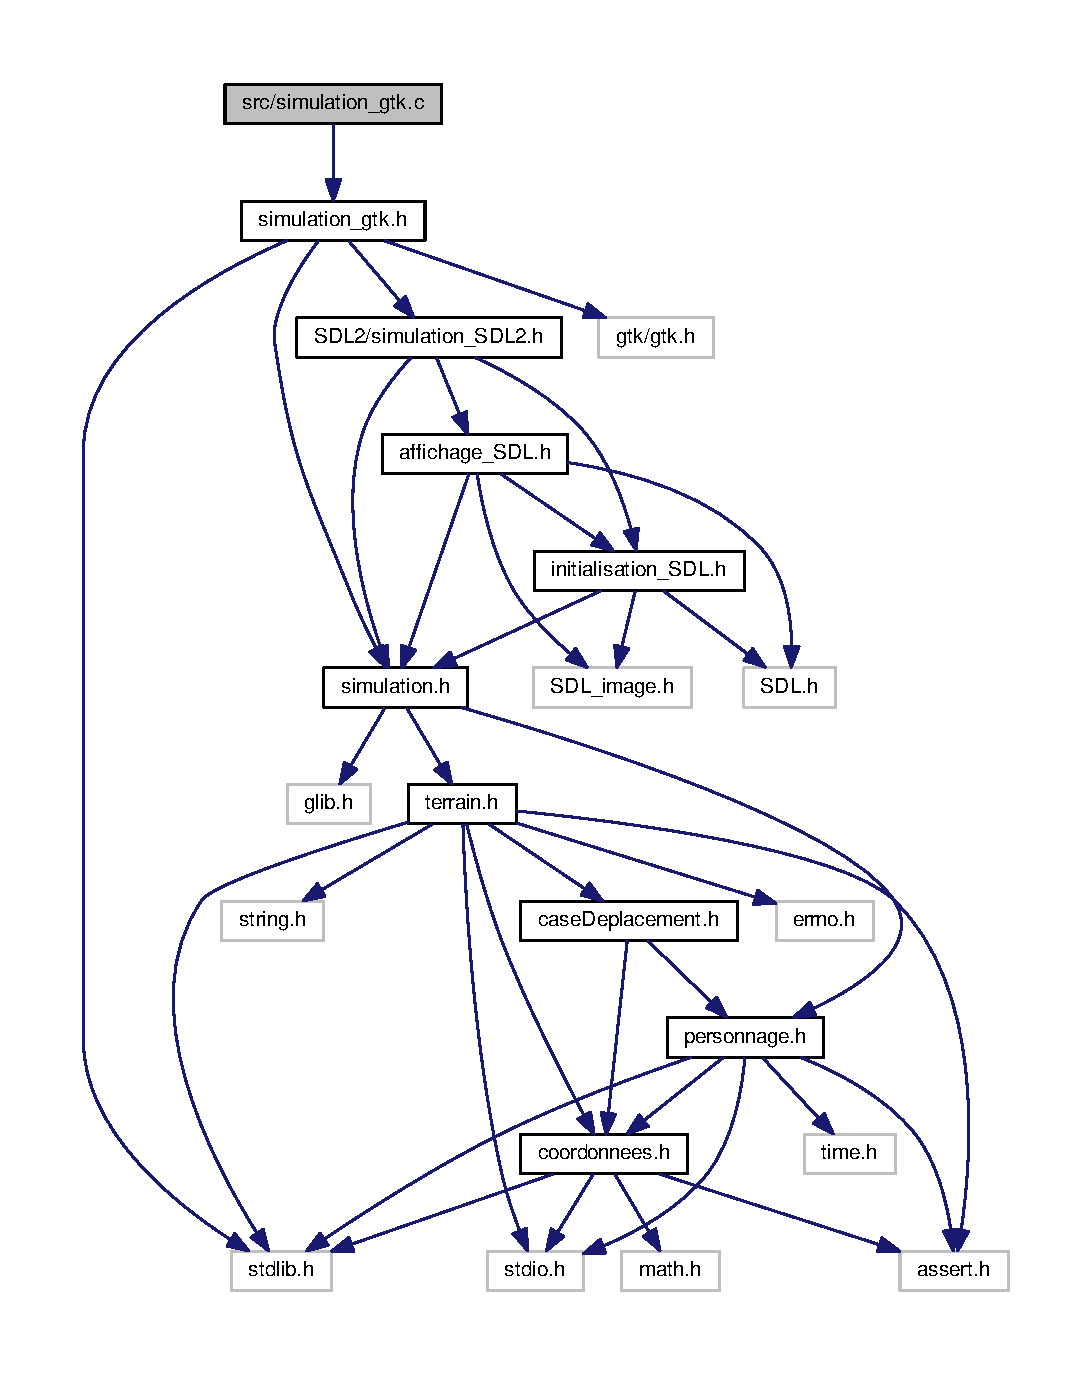
\includegraphics[width=350pt]{simulation__gtk_8c__incl}
\end{center}
\end{figure}
\subsection*{Fonctions}
\begin{DoxyCompactItemize}
\item 
void \hyperlink{simulation__gtk_8c_a2a954c02c0f9c5e4f51691a5cc4b5f74}{start\+Gtk\+Main} (int argc, char $\ast$$\ast$argv)
\begin{DoxyCompactList}\small\item\em Lance l\textquotesingle{}interface G\+TK. \end{DoxyCompactList}\item 
G\+\_\+\+M\+O\+D\+U\+L\+E\+\_\+\+E\+X\+P\+O\+RT gboolean \hyperlink{simulation__gtk_8c_a1339d01047fd730504f9c50db102f205}{bouton\+\_\+lancement} (Gtk\+Button $\ast$button, \hyperlink{simulation__gtk_8h_a81fbd48bacab447f9e155a83d67d3187}{Ch\+Data} $\ast$data)
\item 
G\+\_\+\+M\+O\+D\+U\+L\+E\+\_\+\+E\+X\+P\+O\+RT gboolean \hyperlink{simulation__gtk_8c_ac4c391d3b013604c3c0cd650c2c3bfc6}{bouton\+\_\+editeur} (Gtk\+Button $\ast$button, \hyperlink{simulation__gtk_8h_a81fbd48bacab447f9e155a83d67d3187}{Ch\+Data} $\ast$data)
\end{DoxyCompactItemize}


\subsection{Documentation des fonctions}
\index{simulation\+\_\+gtk.\+c@{simulation\+\_\+gtk.\+c}!bouton\+\_\+editeur@{bouton\+\_\+editeur}}
\index{bouton\+\_\+editeur@{bouton\+\_\+editeur}!simulation\+\_\+gtk.\+c@{simulation\+\_\+gtk.\+c}}
\subsubsection[{\texorpdfstring{bouton\+\_\+editeur(\+Gtk\+Button $\ast$button, Ch\+Data $\ast$data)}{bouton_editeur(GtkButton *button, ChData *data)}}]{\setlength{\rightskip}{0pt plus 5cm}G\+\_\+\+M\+O\+D\+U\+L\+E\+\_\+\+E\+X\+P\+O\+RT gboolean bouton\+\_\+editeur (
\begin{DoxyParamCaption}
\item[{Gtk\+Button $\ast$}]{button, }
\item[{{\bf Ch\+Data} $\ast$}]{data}
\end{DoxyParamCaption}
)}\hypertarget{simulation__gtk_8c_ac4c391d3b013604c3c0cd650c2c3bfc6}{}\label{simulation__gtk_8c_ac4c391d3b013604c3c0cd650c2c3bfc6}
\index{simulation\+\_\+gtk.\+c@{simulation\+\_\+gtk.\+c}!bouton\+\_\+lancement@{bouton\+\_\+lancement}}
\index{bouton\+\_\+lancement@{bouton\+\_\+lancement}!simulation\+\_\+gtk.\+c@{simulation\+\_\+gtk.\+c}}
\subsubsection[{\texorpdfstring{bouton\+\_\+lancement(\+Gtk\+Button $\ast$button, Ch\+Data $\ast$data)}{bouton_lancement(GtkButton *button, ChData *data)}}]{\setlength{\rightskip}{0pt plus 5cm}G\+\_\+\+M\+O\+D\+U\+L\+E\+\_\+\+E\+X\+P\+O\+RT gboolean bouton\+\_\+lancement (
\begin{DoxyParamCaption}
\item[{Gtk\+Button $\ast$}]{button, }
\item[{{\bf Ch\+Data} $\ast$}]{data}
\end{DoxyParamCaption}
)}\hypertarget{simulation__gtk_8c_a1339d01047fd730504f9c50db102f205}{}\label{simulation__gtk_8c_a1339d01047fd730504f9c50db102f205}
\index{simulation\+\_\+gtk.\+c@{simulation\+\_\+gtk.\+c}!start\+Gtk\+Main@{start\+Gtk\+Main}}
\index{start\+Gtk\+Main@{start\+Gtk\+Main}!simulation\+\_\+gtk.\+c@{simulation\+\_\+gtk.\+c}}
\subsubsection[{\texorpdfstring{start\+Gtk\+Main(int argc, char $\ast$$\ast$argv)}{startGtkMain(int argc, char **argv)}}]{\setlength{\rightskip}{0pt plus 5cm}void start\+Gtk\+Main (
\begin{DoxyParamCaption}
\item[{int}]{argc, }
\item[{char $\ast$$\ast$}]{argv}
\end{DoxyParamCaption}
)}\hypertarget{simulation__gtk_8c_a2a954c02c0f9c5e4f51691a5cc4b5f74}{}\label{simulation__gtk_8c_a2a954c02c0f9c5e4f51691a5cc4b5f74}


Lance l\textquotesingle{}interface G\+TK. 


\hypertarget{simulation__gtk_8h}{}\section{Référence du fichier src/simulation\+\_\+gtk.h}
\label{simulation__gtk_8h}\index{src/simulation\+\_\+gtk.\+h@{src/simulation\+\_\+gtk.\+h}}


Définit les fonction appelant à la librairie gtk.  


{\ttfamily \#include $<$stdlib.\+h$>$}\\*
{\ttfamily \#include $<$gtk/gtk.\+h$>$}\\*
{\ttfamily \#include \char`\"{}simulation.\+h\char`\"{}}\\*
{\ttfamily \#include \char`\"{}S\+D\+L2/simulation\+\_\+\+S\+D\+L2.\+h\char`\"{}}\\*
Graphe des dépendances par inclusion de simulation\+\_\+gtk.\+h\+:
\nopagebreak
\begin{figure}[H]
\begin{center}
\leavevmode
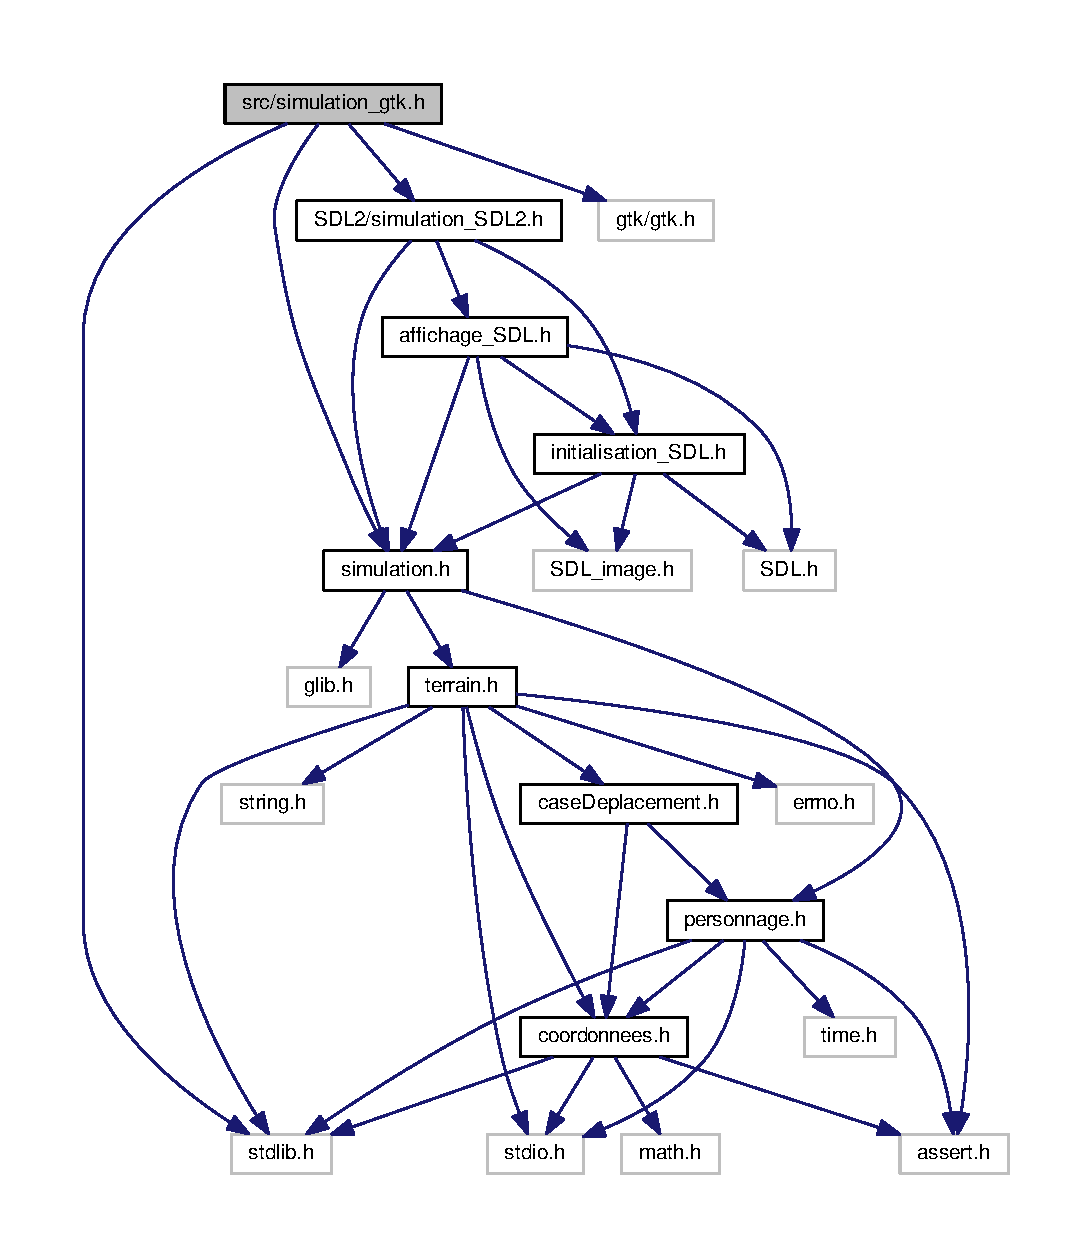
\includegraphics[width=350pt]{simulation__gtk_8h__incl}
\end{center}
\end{figure}
Ce graphe montre quels fichiers incluent directement ou indirectement ce fichier \+:
\nopagebreak
\begin{figure}[H]
\begin{center}
\leavevmode
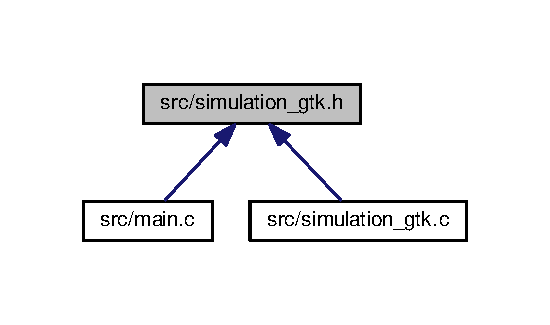
\includegraphics[width=264pt]{simulation__gtk_8h__dep__incl}
\end{center}
\end{figure}
\subsection*{Classes}
\begin{DoxyCompactItemize}
\item 
struct \hyperlink{struct__ChData}{\+\_\+\+Ch\+Data}
\end{DoxyCompactItemize}
\subsection*{Définitions de type}
\begin{DoxyCompactItemize}
\item 
typedef struct \hyperlink{struct__ChData}{\+\_\+\+Ch\+Data} \hyperlink{simulation__gtk_8h_a81fbd48bacab447f9e155a83d67d3187}{Ch\+Data}
\end{DoxyCompactItemize}
\subsection*{Fonctions}
\begin{DoxyCompactItemize}
\item 
void \hyperlink{simulation__gtk_8h_a2a954c02c0f9c5e4f51691a5cc4b5f74}{start\+Gtk\+Main} (int argc, char $\ast$$\ast$argv)
\begin{DoxyCompactList}\small\item\em Lance l\textquotesingle{}interface G\+TK. \end{DoxyCompactList}\end{DoxyCompactItemize}


\subsection{Description détaillée}
Définit les fonction appelant à la librairie gtk. 



\subsection{Documentation des définitions de type}
\index{simulation\+\_\+gtk.\+h@{simulation\+\_\+gtk.\+h}!Ch\+Data@{Ch\+Data}}
\index{Ch\+Data@{Ch\+Data}!simulation\+\_\+gtk.\+h@{simulation\+\_\+gtk.\+h}}
\subsubsection[{\texorpdfstring{Ch\+Data}{ChData}}]{\setlength{\rightskip}{0pt plus 5cm}typedef struct {\bf \+\_\+\+Ch\+Data} {\bf Ch\+Data}}\hypertarget{simulation__gtk_8h_a81fbd48bacab447f9e155a83d67d3187}{}\label{simulation__gtk_8h_a81fbd48bacab447f9e155a83d67d3187}


\subsection{Documentation des fonctions}
\index{simulation\+\_\+gtk.\+h@{simulation\+\_\+gtk.\+h}!start\+Gtk\+Main@{start\+Gtk\+Main}}
\index{start\+Gtk\+Main@{start\+Gtk\+Main}!simulation\+\_\+gtk.\+h@{simulation\+\_\+gtk.\+h}}
\subsubsection[{\texorpdfstring{start\+Gtk\+Main(int argc, char $\ast$$\ast$argv)}{startGtkMain(int argc, char **argv)}}]{\setlength{\rightskip}{0pt plus 5cm}void start\+Gtk\+Main (
\begin{DoxyParamCaption}
\item[{int}]{argc, }
\item[{char $\ast$$\ast$}]{argv}
\end{DoxyParamCaption}
)}\hypertarget{simulation__gtk_8h_a2a954c02c0f9c5e4f51691a5cc4b5f74}{}\label{simulation__gtk_8h_a2a954c02c0f9c5e4f51691a5cc4b5f74}


Lance l\textquotesingle{}interface G\+TK. 


\hypertarget{simulation__ncurses_8c}{}\section{Référence du fichier src/simulation\+\_\+ncurses.c}
\label{simulation__ncurses_8c}\index{src/simulation\+\_\+ncurses.\+c@{src/simulation\+\_\+ncurses.\+c}}
{\ttfamily \#include \char`\"{}simulation\+\_\+ncurses.\+h\char`\"{}}\\*
Graphe des dépendances par inclusion de simulation\+\_\+ncurses.\+c\+:\nopagebreak
\begin{figure}[H]
\begin{center}
\leavevmode
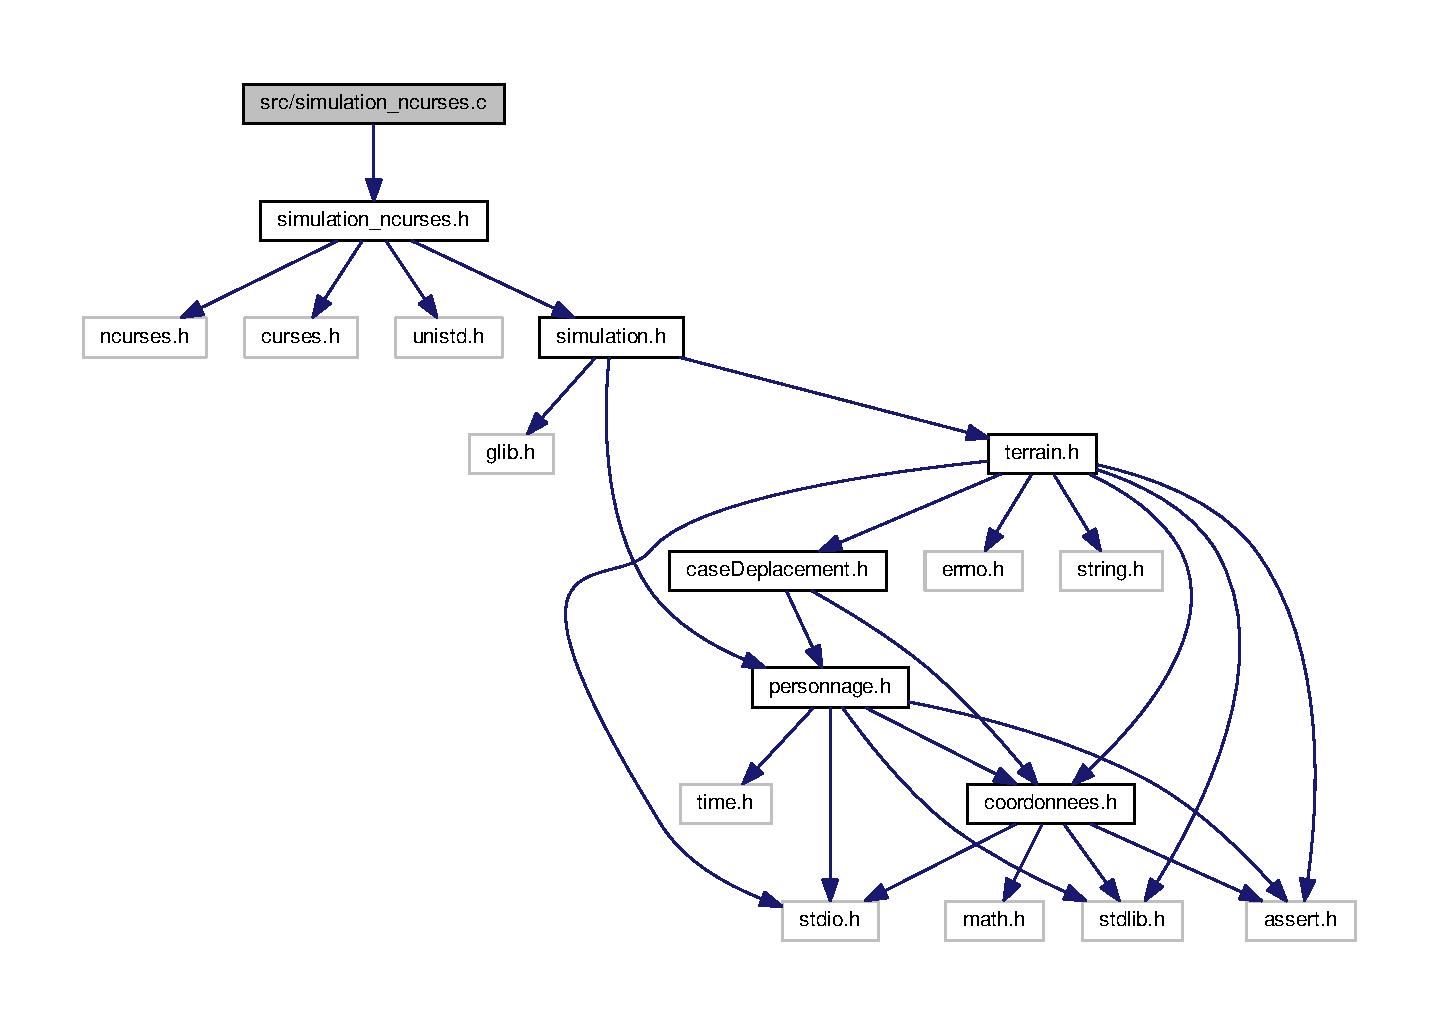
\includegraphics[width=350pt]{simulation__ncurses_8c__incl}
\end{center}
\end{figure}
\subsection*{Fonctions}
\begin{DoxyCompactItemize}
\item 
void \hyperlink{simulation__ncurses_8c_ad87e60f7206c72fa4de844c8eeb7d4af}{lancer\+Simulation\+Ncurses} (char $\ast$nom\+Fic)
\item 
void \hyperlink{simulation__ncurses_8c_a599336149780efa3df29153dd37534ea}{affiche\+Grille} (\hyperlink{simulation_8h_a1ab3bf4791ab776bb4bd460dcce3e8d7}{Simulation} $\ast$p\+Sim)
\item 
void \hyperlink{simulation__ncurses_8c_ae05374caba800b8819342b3006aacbfc}{boucle\+Simulation} (\hyperlink{simulation_8h_a1ab3bf4791ab776bb4bd460dcce3e8d7}{Simulation} $\ast$p\+Sim)
\end{DoxyCompactItemize}


\subsection{Documentation des fonctions}
\index{simulation\+\_\+ncurses.\+c@{simulation\+\_\+ncurses.\+c}!affiche\+Grille@{affiche\+Grille}}
\index{affiche\+Grille@{affiche\+Grille}!simulation\+\_\+ncurses.\+c@{simulation\+\_\+ncurses.\+c}}
\subsubsection[{\texorpdfstring{affiche\+Grille(\+Simulation $\ast$p\+Sim)}{afficheGrille(Simulation *pSim)}}]{\setlength{\rightskip}{0pt plus 5cm}void affiche\+Grille (
\begin{DoxyParamCaption}
\item[{{\bf Simulation} $\ast$}]{p\+Sim}
\end{DoxyParamCaption}
)}\hypertarget{simulation__ncurses_8c_a599336149780efa3df29153dd37534ea}{}\label{simulation__ncurses_8c_a599336149780efa3df29153dd37534ea}
\index{simulation\+\_\+ncurses.\+c@{simulation\+\_\+ncurses.\+c}!boucle\+Simulation@{boucle\+Simulation}}
\index{boucle\+Simulation@{boucle\+Simulation}!simulation\+\_\+ncurses.\+c@{simulation\+\_\+ncurses.\+c}}
\subsubsection[{\texorpdfstring{boucle\+Simulation(\+Simulation $\ast$p\+Sim)}{boucleSimulation(Simulation *pSim)}}]{\setlength{\rightskip}{0pt plus 5cm}void boucle\+Simulation (
\begin{DoxyParamCaption}
\item[{{\bf Simulation} $\ast$}]{p\+Sim}
\end{DoxyParamCaption}
)}\hypertarget{simulation__ncurses_8c_ae05374caba800b8819342b3006aacbfc}{}\label{simulation__ncurses_8c_ae05374caba800b8819342b3006aacbfc}
\index{simulation\+\_\+ncurses.\+c@{simulation\+\_\+ncurses.\+c}!lancer\+Simulation\+Ncurses@{lancer\+Simulation\+Ncurses}}
\index{lancer\+Simulation\+Ncurses@{lancer\+Simulation\+Ncurses}!simulation\+\_\+ncurses.\+c@{simulation\+\_\+ncurses.\+c}}
\subsubsection[{\texorpdfstring{lancer\+Simulation\+Ncurses(char $\ast$nom\+Fic)}{lancerSimulationNcurses(char *nomFic)}}]{\setlength{\rightskip}{0pt plus 5cm}void lancer\+Simulation\+Ncurses (
\begin{DoxyParamCaption}
\item[{char $\ast$}]{nom\+Fic}
\end{DoxyParamCaption}
)}\hypertarget{simulation__ncurses_8c_ad87e60f7206c72fa4de844c8eeb7d4af}{}\label{simulation__ncurses_8c_ad87e60f7206c72fa4de844c8eeb7d4af}

\hypertarget{simulation__ncurses_8h}{}\section{Référence du fichier src/simulation\+\_\+ncurses.h}
\label{simulation__ncurses_8h}\index{src/simulation\+\_\+ncurses.\+h@{src/simulation\+\_\+ncurses.\+h}}


Définit les fonction appelant à la librairie n\+Curses.  


{\ttfamily \#include $<$ncurses.\+h$>$}\\*
{\ttfamily \#include $<$curses.\+h$>$}\\*
{\ttfamily \#include $<$unistd.\+h$>$}\\*
{\ttfamily \#include \char`\"{}simulation.\+h\char`\"{}}\\*
Graphe des dépendances par inclusion de simulation\+\_\+ncurses.\+h\+:\nopagebreak
\begin{figure}[H]
\begin{center}
\leavevmode
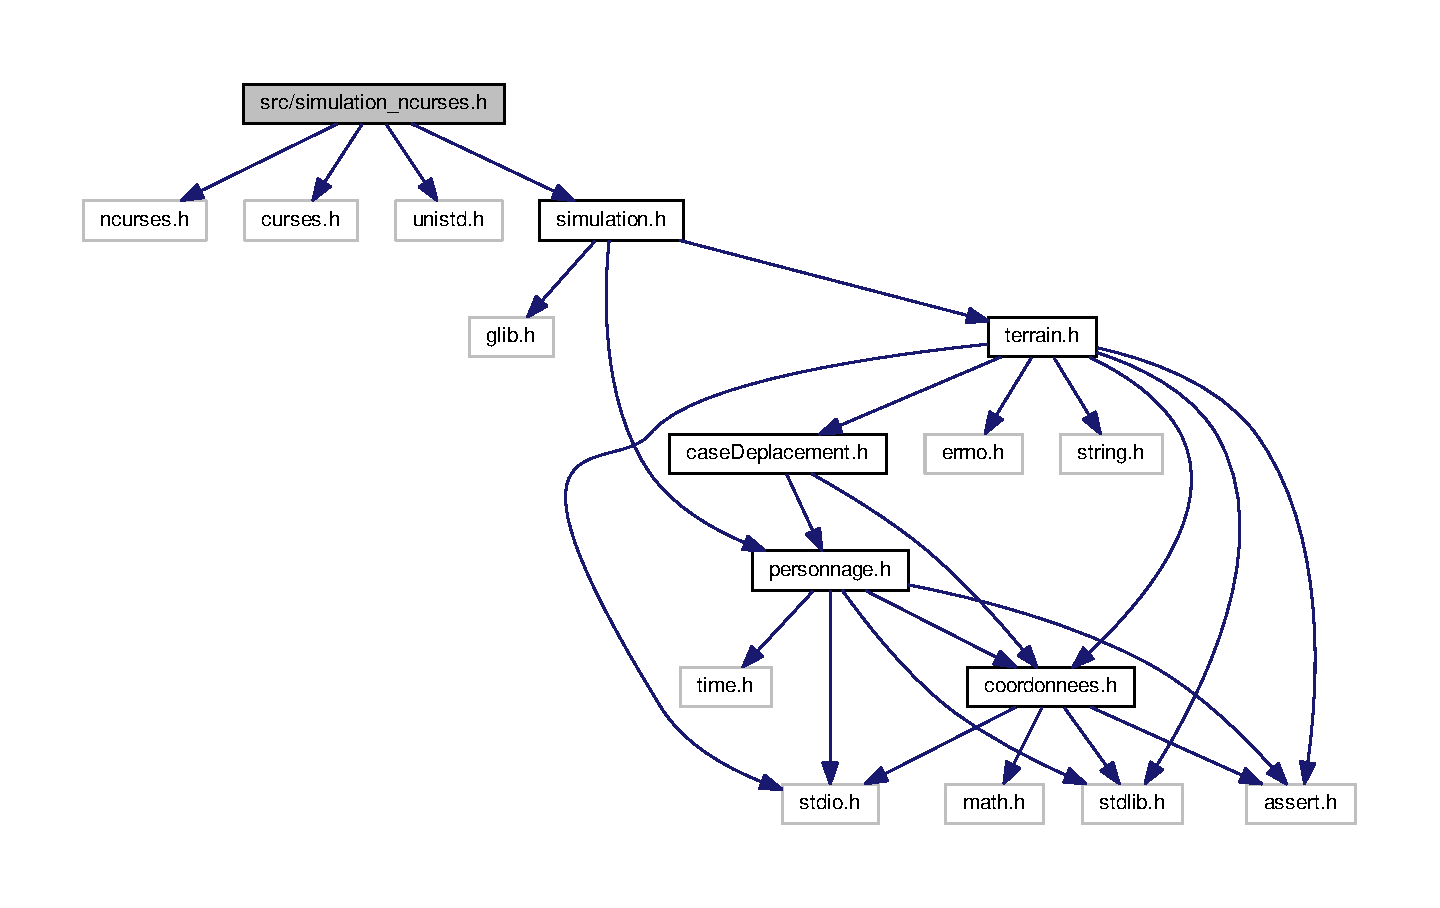
\includegraphics[width=350pt]{simulation__ncurses_8h__incl}
\end{center}
\end{figure}
Ce graphe montre quels fichiers incluent directement ou indirectement ce fichier \+:\nopagebreak
\begin{figure}[H]
\begin{center}
\leavevmode
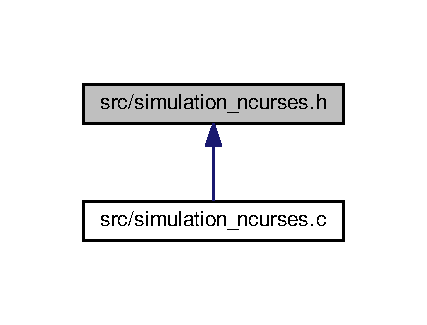
\includegraphics[width=205pt]{simulation__ncurses_8h__dep__incl}
\end{center}
\end{figure}
\subsection*{Fonctions}
\begin{DoxyCompactItemize}
\item 
void \hyperlink{simulation__ncurses_8h_ad87e60f7206c72fa4de844c8eeb7d4af}{lancer\+Simulation\+Ncurses} (char $\ast$nom\+Fic)
\item 
void \hyperlink{simulation__ncurses_8h_a599336149780efa3df29153dd37534ea}{affiche\+Grille} (\hyperlink{simulation_8h_a1ab3bf4791ab776bb4bd460dcce3e8d7}{Simulation} $\ast$p\+Sim)
\item 
void \hyperlink{simulation__ncurses_8h_ae05374caba800b8819342b3006aacbfc}{boucle\+Simulation} (\hyperlink{simulation_8h_a1ab3bf4791ab776bb4bd460dcce3e8d7}{Simulation} $\ast$p\+Sim)
\end{DoxyCompactItemize}


\subsection{Description détaillée}
Définit les fonction appelant à la librairie n\+Curses. 



\subsection{Documentation des fonctions}
\index{simulation\+\_\+ncurses.\+h@{simulation\+\_\+ncurses.\+h}!affiche\+Grille@{affiche\+Grille}}
\index{affiche\+Grille@{affiche\+Grille}!simulation\+\_\+ncurses.\+h@{simulation\+\_\+ncurses.\+h}}
\subsubsection[{\texorpdfstring{affiche\+Grille(\+Simulation $\ast$p\+Sim)}{afficheGrille(Simulation *pSim)}}]{\setlength{\rightskip}{0pt plus 5cm}void affiche\+Grille (
\begin{DoxyParamCaption}
\item[{{\bf Simulation} $\ast$}]{p\+Sim}
\end{DoxyParamCaption}
)}\hypertarget{simulation__ncurses_8h_a599336149780efa3df29153dd37534ea}{}\label{simulation__ncurses_8h_a599336149780efa3df29153dd37534ea}
\index{simulation\+\_\+ncurses.\+h@{simulation\+\_\+ncurses.\+h}!boucle\+Simulation@{boucle\+Simulation}}
\index{boucle\+Simulation@{boucle\+Simulation}!simulation\+\_\+ncurses.\+h@{simulation\+\_\+ncurses.\+h}}
\subsubsection[{\texorpdfstring{boucle\+Simulation(\+Simulation $\ast$p\+Sim)}{boucleSimulation(Simulation *pSim)}}]{\setlength{\rightskip}{0pt plus 5cm}void boucle\+Simulation (
\begin{DoxyParamCaption}
\item[{{\bf Simulation} $\ast$}]{p\+Sim}
\end{DoxyParamCaption}
)}\hypertarget{simulation__ncurses_8h_ae05374caba800b8819342b3006aacbfc}{}\label{simulation__ncurses_8h_ae05374caba800b8819342b3006aacbfc}
\index{simulation\+\_\+ncurses.\+h@{simulation\+\_\+ncurses.\+h}!lancer\+Simulation\+Ncurses@{lancer\+Simulation\+Ncurses}}
\index{lancer\+Simulation\+Ncurses@{lancer\+Simulation\+Ncurses}!simulation\+\_\+ncurses.\+h@{simulation\+\_\+ncurses.\+h}}
\subsubsection[{\texorpdfstring{lancer\+Simulation\+Ncurses(char $\ast$nom\+Fic)}{lancerSimulationNcurses(char *nomFic)}}]{\setlength{\rightskip}{0pt plus 5cm}void lancer\+Simulation\+Ncurses (
\begin{DoxyParamCaption}
\item[{char $\ast$}]{nom\+Fic}
\end{DoxyParamCaption}
)}\hypertarget{simulation__ncurses_8h_ad87e60f7206c72fa4de844c8eeb7d4af}{}\label{simulation__ncurses_8h_ad87e60f7206c72fa4de844c8eeb7d4af}

\hypertarget{terrain_8c}{}\section{Référence du fichier src/terrain.c}
\label{terrain_8c}\index{src/terrain.\+c@{src/terrain.\+c}}
{\ttfamily \#include \char`\"{}terrain.\+h\char`\"{}}\\*
Graphe des dépendances par inclusion de terrain.\+c\+:\nopagebreak
\begin{figure}[H]
\begin{center}
\leavevmode
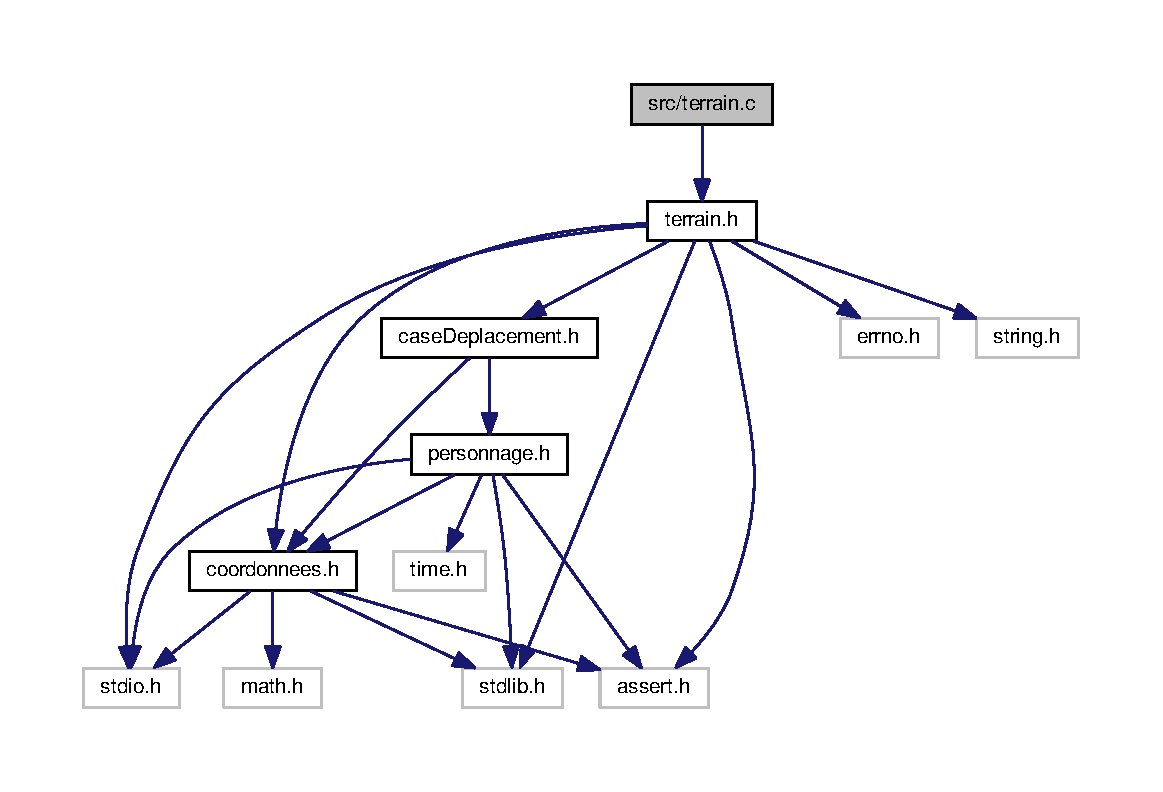
\includegraphics[width=350pt]{terrain_8c__incl}
\end{center}
\end{figure}
\subsection*{Fonctions}
\begin{DoxyCompactItemize}
\item 
void \hyperlink{terrain_8c_aa4dcb232d424b858d3f01f4951d411d4}{set\+Dim\+\_\+terr} (int x, int y, \hyperlink{terrain_8h_a11bbfdc6f8212f3246205cc0e7134136}{Terrain} $\ast$p\+Terrain)
\begin{DoxyCompactList}\small\item\em Edition de X et de Y dans la structure. \end{DoxyCompactList}\item 
void \hyperlink{terrain_8c_afd0cd33d4703b04455c6b118a3936e63}{set\+Nom\+Terrain\+\_\+terr} (char $\ast$nom, \hyperlink{terrain_8h_a11bbfdc6f8212f3246205cc0e7134136}{Terrain} $\ast$p\+Terrain)
\item 
void \hyperlink{terrain_8c_a97c9cc766e38342e3425653e89b6f46c}{set\+Grille\+By\+Coord\+\_\+terr} (\hyperlink{coordonnees_8h_a79929cdfee7bd985a5e4e25276bb3ba9}{Coordonnees} $\ast$coord, \hyperlink{terrain_8h_a11bbfdc6f8212f3246205cc0e7134136}{Terrain} $\ast$p\+Terrain, \hyperlink{caseDeplacement_8h_aeab4f22b99f0db8b549dab4e46e3ead4}{case\+Deplacement} $\ast$case\+Dep)
\begin{DoxyCompactList}\small\item\em Change la case de deplacement de la grille au coordonnées données. \end{DoxyCompactList}\item 
void \hyperlink{terrain_8c_ad15a1365737240775ff8425378834fd6}{set\+Grille\+By\+X\+Y\+\_\+terr} (int x, int y, \hyperlink{terrain_8h_a11bbfdc6f8212f3246205cc0e7134136}{Terrain} $\ast$p\+Terrain, \hyperlink{caseDeplacement_8h_aeab4f22b99f0db8b549dab4e46e3ead4}{case\+Deplacement} $\ast$case\+Dep)
\begin{DoxyCompactList}\small\item\em Edition du type de la grille du terrain au coordonnées X/Y. \end{DoxyCompactList}\item 
int \hyperlink{terrain_8c_a09bd83bff226b5e25af2e9dfb160260c}{get\+Dim\+X\+\_\+terr} (\hyperlink{terrain_8h_a11bbfdc6f8212f3246205cc0e7134136}{Terrain} $\ast$p\+Terrain)
\begin{DoxyCompactList}\small\item\em Recupère la dimension en X de la structure Terrain. \end{DoxyCompactList}\item 
int \hyperlink{terrain_8c_a1fd39032dab5b6e3556883315a7868c5}{get\+Dim\+Y\+\_\+terr} (\hyperlink{terrain_8h_a11bbfdc6f8212f3246205cc0e7134136}{Terrain} $\ast$p\+Terrain)
\begin{DoxyCompactList}\small\item\em Recupère la dimension en Y de la structure Terrain. \end{DoxyCompactList}\item 
char $\ast$ \hyperlink{terrain_8c_aa2d2d29116636980d1b3f9f0a7a85ae0}{get\+Nom\+Terrain\+\_\+terr} (\hyperlink{terrain_8h_a11bbfdc6f8212f3246205cc0e7134136}{Terrain} $\ast$p\+Terrain)
\begin{DoxyCompactList}\small\item\em Recupère le nom de la structure Terrain. \end{DoxyCompactList}\item 
\hyperlink{caseDeplacement_8h_aeab4f22b99f0db8b549dab4e46e3ead4}{case\+Deplacement} $\ast$ \hyperlink{terrain_8c_a3b01a560ba891070ee62880f2739ea5b}{get\+Grille\+By\+X\+Y\+\_\+terr} (int x, int y, \hyperlink{terrain_8h_a11bbfdc6f8212f3246205cc0e7134136}{Terrain} $\ast$p\+Terrain)
\begin{DoxyCompactList}\small\item\em Recupere la case de deplacement de la grille au point X/Y. \end{DoxyCompactList}\item 
\hyperlink{caseDeplacement_8h_aeab4f22b99f0db8b549dab4e46e3ead4}{case\+Deplacement} $\ast$ \hyperlink{terrain_8c_a16b89b3a3faa749c3fa4d6bf03791487}{get\+Grille\+By\+Coord\+\_\+terr} (\hyperlink{coordonnees_8h_a79929cdfee7bd985a5e4e25276bb3ba9}{Coordonnees} $\ast$coord, \hyperlink{terrain_8h_a11bbfdc6f8212f3246205cc0e7134136}{Terrain} $\ast$p\+Terrain)
\begin{DoxyCompactList}\small\item\em Recupere la case de deplacement de la grille au coordonnées données. \end{DoxyCompactList}\item 
\hyperlink{caseDeplacement_8h_aeab4f22b99f0db8b549dab4e46e3ead4}{case\+Deplacement} $\ast$ \hyperlink{terrain_8c_af1ce19edb047ad98f13eb599869cc462}{get\+Case\+Bas\+By\+Coord} (\hyperlink{coordonnees_8h_a79929cdfee7bd985a5e4e25276bb3ba9}{Coordonnees} $\ast$coord, \hyperlink{terrain_8h_a11bbfdc6f8212f3246205cc0e7134136}{Terrain} $\ast$p\+Terrain)
\begin{DoxyCompactList}\small\item\em Recupere la case de deplacement de la grille en dessous des coordonée. \end{DoxyCompactList}\item 
\hyperlink{caseDeplacement_8h_aeab4f22b99f0db8b549dab4e46e3ead4}{case\+Deplacement} $\ast$ \hyperlink{terrain_8c_a7fe6b65294f394be319ead817fd6ec1e}{get\+Case\+Haut\+By\+Coord} (\hyperlink{coordonnees_8h_a79929cdfee7bd985a5e4e25276bb3ba9}{Coordonnees} $\ast$coord, \hyperlink{terrain_8h_a11bbfdc6f8212f3246205cc0e7134136}{Terrain} $\ast$p\+Terrain)
\begin{DoxyCompactList}\small\item\em Recupere la case de deplacement de la grille en haut des coordonée. \end{DoxyCompactList}\item 
\hyperlink{caseDeplacement_8h_aeab4f22b99f0db8b549dab4e46e3ead4}{case\+Deplacement} $\ast$ \hyperlink{terrain_8c_ac71d16722a67e2a956f88e60e445efe6}{get\+Case\+Gauche\+By\+Coord} (\hyperlink{coordonnees_8h_a79929cdfee7bd985a5e4e25276bb3ba9}{Coordonnees} $\ast$coord, \hyperlink{terrain_8h_a11bbfdc6f8212f3246205cc0e7134136}{Terrain} $\ast$p\+Terrain)
\begin{DoxyCompactList}\small\item\em Recupere la case de deplacement de la grille a gauche des coordonée. \end{DoxyCompactList}\item 
\hyperlink{caseDeplacement_8h_aeab4f22b99f0db8b549dab4e46e3ead4}{case\+Deplacement} $\ast$ \hyperlink{terrain_8c_a454f9cef12a6b3be9691dff9ee195125}{get\+Case\+Droite\+By\+Coord} (\hyperlink{coordonnees_8h_a79929cdfee7bd985a5e4e25276bb3ba9}{Coordonnees} $\ast$coord, \hyperlink{terrain_8h_a11bbfdc6f8212f3246205cc0e7134136}{Terrain} $\ast$p\+Terrain)
\begin{DoxyCompactList}\small\item\em Recupere la case de deplacement de la grille a droite des coordonée. \end{DoxyCompactList}\item 
char \hyperlink{terrain_8c_af7944caa30120319f283d3818ce1b346}{place\+Perso\+By\+Coord} (\hyperlink{personnage_8h_abd5c92a453bbf273f753b3f5b99da9e7}{Perso} $\ast$p\+Perso, \hyperlink{coordonnees_8h_a79929cdfee7bd985a5e4e25276bb3ba9}{Coordonnees} $\ast$coord, \hyperlink{terrain_8h_a11bbfdc6f8212f3246205cc0e7134136}{Terrain} $\ast$p\+Terrain)
\item 
\hyperlink{personnage_8h_abd5c92a453bbf273f753b3f5b99da9e7}{Perso} $\ast$ \hyperlink{terrain_8c_ae5f55773094ee4c234974d40b3287856}{cree\+Perso\+Terrain\+Rand} (\hyperlink{terrain_8h_a11bbfdc6f8212f3246205cc0e7134136}{Terrain} $\ast$p\+Terrain, enum \hyperlink{personnage_8h_a3f6a2951aa3d5d428dd6d61e74db0d75}{type\+Perso} type, int id\+Perso)
\item 
void \hyperlink{terrain_8c_aad20d9f641c2045b6556280495340013}{terrain\+Ajout\+Mur\+Tour} (\hyperlink{terrain_8h_a11bbfdc6f8212f3246205cc0e7134136}{Terrain} $\ast$p\+Terrain)
\begin{DoxyCompactList}\small\item\em Ajoute des mur sur les bord du terrain. \end{DoxyCompactList}\item 
void \hyperlink{terrain_8c_a3983dae49e4000872233e7d83205a247}{terrain\+Init\+Grille\+\_\+terr} (\hyperlink{terrain_8h_a11bbfdc6f8212f3246205cc0e7134136}{Terrain} $\ast$p\+Terrain)
\begin{DoxyCompactList}\small\item\em Initialise la grille d\textquotesingle{}un terrain. \end{DoxyCompactList}\item 
\hyperlink{terrain_8h_a11bbfdc6f8212f3246205cc0e7134136}{Terrain} $\ast$ \hyperlink{terrain_8c_a18be630674285fc320507f21282be35f}{terrain\+Creer\+\_\+terr} (int dimX, int dimY, char nom\+Terrain\mbox{[}\hyperlink{terrain_8h_a5f41c70ea486e890717560da2605f309}{M\+A\+X\+\_\+\+C\+H\+A\+R\+\_\+\+N\+O\+M\+\_\+\+T\+E\+R\+R\+A\+IN}\mbox{]})
\begin{DoxyCompactList}\small\item\em Creer un terrain avec les dimension et le nom choisi et initialise sa grille en appelant Terrain\+Init\+Grille. \end{DoxyCompactList}\item 
void \hyperlink{terrain_8c_adcec4a15a3bf0455ad742bdcd940f2cb}{testament\+Terrain\+\_\+terr} (\hyperlink{terrain_8h_a11bbfdc6f8212f3246205cc0e7134136}{Terrain} $\ast$p\+Terrain)
\begin{DoxyCompactList}\small\item\em Libere la mémoire occupé par un terrain. \end{DoxyCompactList}\item 
char \hyperlink{terrain_8c_a97c090e1c8063d66314f3be8b159e2cd}{est\+Dans\+Terrain\+\_\+terr} (\hyperlink{terrain_8h_a11bbfdc6f8212f3246205cc0e7134136}{Terrain} $\ast$p\+Terrain, \hyperlink{coordonnees_8h_a79929cdfee7bd985a5e4e25276bb3ba9}{Coordonnees} $\ast$p\+Coord)
\begin{DoxyCompactList}\small\item\em Verifie si des coordonnées appartiennent au terrain. \end{DoxyCompactList}\item 
char \hyperlink{terrain_8c_a8d3c2c01aa89e785014ad2209d990c0a}{verif\+Deplacement\+Bas\+\_\+perso} (\hyperlink{personnage_8h_abd5c92a453bbf273f753b3f5b99da9e7}{Perso} $\ast$p\+Perso, \hyperlink{terrain_8h_a11bbfdc6f8212f3246205cc0e7134136}{Terrain} $\ast$p\+Terrain)
\begin{DoxyCompactList}\small\item\em Verifie si le personnage peut aller en bas. \end{DoxyCompactList}\item 
char \hyperlink{terrain_8c_a9fba0242ab21d6632a379cd00ee20f0e}{verif\+Deplacement\+Haut\+\_\+perso} (\hyperlink{personnage_8h_abd5c92a453bbf273f753b3f5b99da9e7}{Perso} $\ast$p\+Perso, \hyperlink{terrain_8h_a11bbfdc6f8212f3246205cc0e7134136}{Terrain} $\ast$p\+Terrain)
\begin{DoxyCompactList}\small\item\em Verifie si le personnage peut aller en haut. \end{DoxyCompactList}\item 
char \hyperlink{terrain_8c_ad8a0578b05cf7d184a2f7c69465cefea}{verif\+Deplacement\+Gauche\+\_\+perso} (\hyperlink{personnage_8h_abd5c92a453bbf273f753b3f5b99da9e7}{Perso} $\ast$p\+Perso, \hyperlink{terrain_8h_a11bbfdc6f8212f3246205cc0e7134136}{Terrain} $\ast$p\+Terrain)
\begin{DoxyCompactList}\small\item\em Verifie si le personnage peut aller a gauche. \end{DoxyCompactList}\item 
char \hyperlink{terrain_8c_a0e34d630de41377283db24f865009ce7}{verif\+Deplacement\+Droite\+\_\+perso} (\hyperlink{personnage_8h_abd5c92a453bbf273f753b3f5b99da9e7}{Perso} $\ast$p\+Perso, \hyperlink{terrain_8h_a11bbfdc6f8212f3246205cc0e7134136}{Terrain} $\ast$p\+Terrain)
\begin{DoxyCompactList}\small\item\em Verifie si le personnage peut aller a droite. \end{DoxyCompactList}\item 
char \hyperlink{terrain_8c_ae09dc2657a465436713dc79a500fbbfd}{deplacement\+Haut\+\_\+perso} (\hyperlink{personnage_8h_abd5c92a453bbf273f753b3f5b99da9e7}{Perso} $\ast$p\+Perso, \hyperlink{terrain_8h_a11bbfdc6f8212f3246205cc0e7134136}{Terrain} $\ast$p\+Terrain)
\begin{DoxyCompactList}\small\item\em Deplace le personnage vers le haut (test avant qu\textquotesingle{}il peut etre deplacé dans ce sens) \end{DoxyCompactList}\item 
char \hyperlink{terrain_8c_a124dcf1c540a5e9f8987153c5629777b}{deplacement\+Bas\+\_\+perso} (\hyperlink{personnage_8h_abd5c92a453bbf273f753b3f5b99da9e7}{Perso} $\ast$p\+Perso, \hyperlink{terrain_8h_a11bbfdc6f8212f3246205cc0e7134136}{Terrain} $\ast$p\+Terrain)
\begin{DoxyCompactList}\small\item\em Deplace le personnage vers le bas (test avant qu\textquotesingle{}il peut etre deplacé dans ce sens) \end{DoxyCompactList}\item 
char \hyperlink{terrain_8c_a8c6c0b998f096f10a0ccad25a136b465}{deplacement\+Gauche\+\_\+perso} (\hyperlink{personnage_8h_abd5c92a453bbf273f753b3f5b99da9e7}{Perso} $\ast$p\+Perso, \hyperlink{terrain_8h_a11bbfdc6f8212f3246205cc0e7134136}{Terrain} $\ast$p\+Terrain)
\begin{DoxyCompactList}\small\item\em Deplace le personnage vers la gauche (test avant qu\textquotesingle{}il peut etre deplacé dans ce sens) \end{DoxyCompactList}\item 
char \hyperlink{terrain_8c_a385bedef7127b250811ce7f0218c66e3}{deplacement\+Droite\+\_\+perso} (\hyperlink{personnage_8h_abd5c92a453bbf273f753b3f5b99da9e7}{Perso} $\ast$p\+Perso, \hyperlink{terrain_8h_a11bbfdc6f8212f3246205cc0e7134136}{Terrain} $\ast$p\+Terrain)
\begin{DoxyCompactList}\small\item\em Deplace le personnage vers la droite (test avant qu\textquotesingle{}il peut etre deplacé dans ce sens) \end{DoxyCompactList}\item 
char \hyperlink{terrain_8c_a50e099874470bb6e68cbd44c68807aa5}{deplacement\+Aleatoire\+\_\+perso} (\hyperlink{personnage_8h_abd5c92a453bbf273f753b3f5b99da9e7}{Perso} $\ast$p\+Perso, \hyperlink{terrain_8h_a11bbfdc6f8212f3246205cc0e7134136}{Terrain} $\ast$p\+Terrain)
\begin{DoxyCompactList}\small\item\em Deplace le personnage dans une direction aléatoire (test avant qu\textquotesingle{}il peut etre deplacé dans ce sens) \end{DoxyCompactList}\item 
char \hyperlink{terrain_8c_ae6548343b2ab3ffd042731aeee925261}{humain\+En\+Haut} (\hyperlink{terrain_8h_a11bbfdc6f8212f3246205cc0e7134136}{Terrain} $\ast$p\+Terrain, \hyperlink{coordonnees_8h_a79929cdfee7bd985a5e4e25276bb3ba9}{Coordonnees} $\ast$coord\+Zombie)
\begin{DoxyCompactList}\small\item\em Verifie si le personnage en haut est un humain. \end{DoxyCompactList}\item 
char \hyperlink{terrain_8c_a50df7bb2b9b06787410c5c3c18c26c7e}{humain\+En\+Bas} (\hyperlink{terrain_8h_a11bbfdc6f8212f3246205cc0e7134136}{Terrain} $\ast$p\+Terrain, \hyperlink{coordonnees_8h_a79929cdfee7bd985a5e4e25276bb3ba9}{Coordonnees} $\ast$coord\+Zombie)
\begin{DoxyCompactList}\small\item\em Verifie si le personnage en bas est un humain. \end{DoxyCompactList}\item 
char \hyperlink{terrain_8c_aa81fd0c9d275c8f8feb23f1400f43e43}{humain\+A\+Gauche} (\hyperlink{terrain_8h_a11bbfdc6f8212f3246205cc0e7134136}{Terrain} $\ast$p\+Terrain, \hyperlink{coordonnees_8h_a79929cdfee7bd985a5e4e25276bb3ba9}{Coordonnees} $\ast$coord\+Zombie)
\begin{DoxyCompactList}\small\item\em Verifie si le personnage a gauche est un humain. \end{DoxyCompactList}\item 
char \hyperlink{terrain_8c_a5f78f92ecac28d78ffd95ba3e04b272d}{humain\+A\+Droite} (\hyperlink{terrain_8h_a11bbfdc6f8212f3246205cc0e7134136}{Terrain} $\ast$p\+Terrain, \hyperlink{coordonnees_8h_a79929cdfee7bd985a5e4e25276bb3ba9}{Coordonnees} $\ast$coord\+Zombie)
\begin{DoxyCompactList}\small\item\em Verifie si le personnage a droite est un humain. \end{DoxyCompactList}\item 
char \hyperlink{terrain_8c_a001f60dfb98bf19a3868269a3a8d4128}{zombie\+En\+Haut} (\hyperlink{terrain_8h_a11bbfdc6f8212f3246205cc0e7134136}{Terrain} $\ast$p\+Terrain, \hyperlink{coordonnees_8h_a79929cdfee7bd985a5e4e25276bb3ba9}{Coordonnees} $\ast$coord\+Zombie)
\begin{DoxyCompactList}\small\item\em Regarde si un zombie se trouve sur la se situant (lire libelé de la fonction) des coordonnées. \end{DoxyCompactList}\item 
char \hyperlink{terrain_8c_ad4328106195808c5a5a40e869ad7a580}{zombie\+En\+Bas} (\hyperlink{terrain_8h_a11bbfdc6f8212f3246205cc0e7134136}{Terrain} $\ast$p\+Terrain, \hyperlink{coordonnees_8h_a79929cdfee7bd985a5e4e25276bb3ba9}{Coordonnees} $\ast$coord\+Zombie)
\begin{DoxyCompactList}\small\item\em Regarde si un zombie se trouve sur la se situant (lire libelé de la fonction) des coordonnées. \end{DoxyCompactList}\item 
char \hyperlink{terrain_8c_af6ccfdc77c33d99a1ae6807aa7c8da8a}{zombie\+A\+Gauche} (\hyperlink{terrain_8h_a11bbfdc6f8212f3246205cc0e7134136}{Terrain} $\ast$p\+Terrain, \hyperlink{coordonnees_8h_a79929cdfee7bd985a5e4e25276bb3ba9}{Coordonnees} $\ast$coord\+Zombie)
\begin{DoxyCompactList}\small\item\em Regarde si un zombie se trouve sur la se situant (lire libelé de la fonction) des coordonnées. \end{DoxyCompactList}\item 
char \hyperlink{terrain_8c_a26dc558207a13a9ee19f2c78d06bf807}{zombie\+A\+Droite} (\hyperlink{terrain_8h_a11bbfdc6f8212f3246205cc0e7134136}{Terrain} $\ast$p\+Terrain, \hyperlink{coordonnees_8h_a79929cdfee7bd985a5e4e25276bb3ba9}{Coordonnees} $\ast$coord\+Zombie)
\begin{DoxyCompactList}\small\item\em Regarde si un zombie se trouve sur la se situant (lire libelé de la fonction) des coordonnées. \end{DoxyCompactList}\item 
char \hyperlink{terrain_8c_ad15a715cc6d4d24dbd1f1b0c5c724c41}{zombie\+En2\+Haut} (\hyperlink{terrain_8h_a11bbfdc6f8212f3246205cc0e7134136}{Terrain} $\ast$p\+Terrain, \hyperlink{coordonnees_8h_a79929cdfee7bd985a5e4e25276bb3ba9}{Coordonnees} $\ast$coord\+Zombie)
\begin{DoxyCompactList}\small\item\em Regarde si un zombie se trouve sur la se situant (lire libelé de la fonction) des coordonnées. \end{DoxyCompactList}\item 
char \hyperlink{terrain_8c_aac1c61b2b5fb5333e2c71072597fe646}{zombie\+En2\+Bas} (\hyperlink{terrain_8h_a11bbfdc6f8212f3246205cc0e7134136}{Terrain} $\ast$p\+Terrain, \hyperlink{coordonnees_8h_a79929cdfee7bd985a5e4e25276bb3ba9}{Coordonnees} $\ast$coord\+Zombie)
\begin{DoxyCompactList}\small\item\em Regarde si un zombie se trouve sur la se situant (lire libelé de la fonction) des coordonnées. \end{DoxyCompactList}\item 
char \hyperlink{terrain_8c_a789481a25a7883fa13a345b5cc86b618}{zombie\+A2\+Gauche} (\hyperlink{terrain_8h_a11bbfdc6f8212f3246205cc0e7134136}{Terrain} $\ast$p\+Terrain, \hyperlink{coordonnees_8h_a79929cdfee7bd985a5e4e25276bb3ba9}{Coordonnees} $\ast$coord\+Zombie)
\begin{DoxyCompactList}\small\item\em Regarde si un zombie se trouve sur la se situant (lire libelé de la fonction) des coordonnées. \end{DoxyCompactList}\item 
char \hyperlink{terrain_8c_a97157bb01d1c0e7eed68d43459410dfc}{zombie\+A2\+Droite} (\hyperlink{terrain_8h_a11bbfdc6f8212f3246205cc0e7134136}{Terrain} $\ast$p\+Terrain, \hyperlink{coordonnees_8h_a79929cdfee7bd985a5e4e25276bb3ba9}{Coordonnees} $\ast$coord\+Zombie)
\begin{DoxyCompactList}\small\item\em Regarde si un zombie se trouve sur la se situant (lire libelé de la fonction) des coordonnées. \end{DoxyCompactList}\item 
char \hyperlink{terrain_8c_ac83836d426c8c3f520114923a555a9bb}{zombie\+HD} (\hyperlink{terrain_8h_a11bbfdc6f8212f3246205cc0e7134136}{Terrain} $\ast$p\+Terrain, \hyperlink{coordonnees_8h_a79929cdfee7bd985a5e4e25276bb3ba9}{Coordonnees} $\ast$coord\+Zombie)
\begin{DoxyCompactList}\small\item\em Regarde si un zombie se trouve sur la se situant (lire libelé de la fonction) des coordonnées. \end{DoxyCompactList}\item 
char \hyperlink{terrain_8c_abba9a396650e8815b0a0d8c093fbc352}{zombie\+BD} (\hyperlink{terrain_8h_a11bbfdc6f8212f3246205cc0e7134136}{Terrain} $\ast$p\+Terrain, \hyperlink{coordonnees_8h_a79929cdfee7bd985a5e4e25276bb3ba9}{Coordonnees} $\ast$coord\+Zombie)
\begin{DoxyCompactList}\small\item\em Regarde si un zombie se trouve sur la se situant (lire libelé de la fonction) des coordonnées. \end{DoxyCompactList}\item 
char \hyperlink{terrain_8c_adc99a25c35fcd27644a47f14129e0278}{zombie\+BG} (\hyperlink{terrain_8h_a11bbfdc6f8212f3246205cc0e7134136}{Terrain} $\ast$p\+Terrain, \hyperlink{coordonnees_8h_a79929cdfee7bd985a5e4e25276bb3ba9}{Coordonnees} $\ast$coord\+Zombie)
\begin{DoxyCompactList}\small\item\em Regarde si un zombie se trouve sur la se situant (lire libelé de la fonction) des coordonnées. \end{DoxyCompactList}\item 
char \hyperlink{terrain_8c_a620533e1f0789251d879b67d9cef829e}{zombie\+HG} (\hyperlink{terrain_8h_a11bbfdc6f8212f3246205cc0e7134136}{Terrain} $\ast$p\+Terrain, \hyperlink{coordonnees_8h_a79929cdfee7bd985a5e4e25276bb3ba9}{Coordonnees} $\ast$coord\+Zombie)
\begin{DoxyCompactList}\small\item\em Regarde si un zombie se trouve sur la se situant (lire libelé de la fonction) des coordonnées. \end{DoxyCompactList}\item 
\hyperlink{personnage_8h_abd5c92a453bbf273f753b3f5b99da9e7}{Perso} $\ast$ \hyperlink{terrain_8c_aef0f8b09c8459770f8901c7f4bc93b6d}{zombie\+Contamine\+Humain} (\hyperlink{personnage_8h_abd5c92a453bbf273f753b3f5b99da9e7}{Perso} $\ast$p\+Zombie, \hyperlink{terrain_8h_a11bbfdc6f8212f3246205cc0e7134136}{Terrain} $\ast$p\+Terrain)
\item 
\hyperlink{personnage_8h_abd5c92a453bbf273f753b3f5b99da9e7}{Perso} $\ast$ \hyperlink{terrain_8c_ad4312194338f3849221a0ae93372b974}{policier\+Tue\+Zombie} (\hyperlink{personnage_8h_abd5c92a453bbf273f753b3f5b99da9e7}{Perso} $\ast$p\+Policier, \hyperlink{terrain_8h_a11bbfdc6f8212f3246205cc0e7134136}{Terrain} $\ast$p\+Terrain)
\item 
void \hyperlink{terrain_8c_aba7a3bbec5c24c999958be6699d8fc11}{afficher\+Grille\+Console} (\hyperlink{terrain_8h_a11bbfdc6f8212f3246205cc0e7134136}{Terrain} $\ast$p\+Terrain)
\begin{DoxyCompactList}\small\item\em Affiche la grille dans la console avec des caractère pour représenter les personnages et murs. \end{DoxyCompactList}\item 
void \hyperlink{terrain_8c_ae74ede311bdc4b21f792dac31ba78834}{terrain\+Creer\+Fichier\+\_\+terr} (\hyperlink{terrain_8h_a11bbfdc6f8212f3246205cc0e7134136}{Terrain} $\ast$p\+Terrain, char $\ast$chemin\+Fichier)
\begin{DoxyCompactList}\small\item\em Créer un fichier terrain à partir du pointeur vers terrain. \end{DoxyCompactList}\item 
\hyperlink{terrain_8h_a11bbfdc6f8212f3246205cc0e7134136}{Terrain} $\ast$ \hyperlink{terrain_8c_af5245ba401335426617e661a1fc0daee}{terrain\+Lire\+Fichier\+\_\+terr} (char $\ast$nom\+Terrain)
\item 
void \hyperlink{terrain_8c_a1ec738cacf8012e6e62410e31cd56d62}{afficher\+Champs} (\hyperlink{terrain_8h_a11bbfdc6f8212f3246205cc0e7134136}{Terrain} $\ast$p\+Terrain)
\begin{DoxyCompactList}\small\item\em Affiche la grille des champs dans la console avec des caractère pour représenter les représenter. \end{DoxyCompactList}\item 
void \hyperlink{terrain_8c_af32214c124513367869c101ca6576bac}{propagation\+Champ} (enum \hyperlink{personnage_8h_a3f6a2951aa3d5d428dd6d61e74db0d75}{type\+Perso} type, int id\+Perso, \hyperlink{coordonnees_8h_a79929cdfee7bd985a5e4e25276bb3ba9}{Coordonnees} $\ast$coord\+Perso, \hyperlink{terrain_8h_a11bbfdc6f8212f3246205cc0e7134136}{Terrain} $\ast$p\+Terrain)
\item 
void \hyperlink{terrain_8c_ae671405a2cab0685307937720369b63f}{test\+Fonctions\+\_\+terr} ()
\begin{DoxyCompactList}\small\item\em Fonctoin de test des fonction du module terrain. \end{DoxyCompactList}\end{DoxyCompactItemize}


\subsection{Documentation des fonctions}
\index{terrain.\+c@{terrain.\+c}!afficher\+Champs@{afficher\+Champs}}
\index{afficher\+Champs@{afficher\+Champs}!terrain.\+c@{terrain.\+c}}
\subsubsection[{\texorpdfstring{afficher\+Champs(\+Terrain $\ast$p\+Terrain)}{afficherChamps(Terrain *pTerrain)}}]{\setlength{\rightskip}{0pt plus 5cm}void afficher\+Champs (
\begin{DoxyParamCaption}
\item[{{\bf Terrain} $\ast$}]{p\+Terrain}
\end{DoxyParamCaption}
)}\hypertarget{terrain_8c_a1ec738cacf8012e6e62410e31cd56d62}{}\label{terrain_8c_a1ec738cacf8012e6e62410e31cd56d62}


Affiche la grille des champs dans la console avec des caractère pour représenter les représenter. 

\index{terrain.\+c@{terrain.\+c}!afficher\+Grille\+Console@{afficher\+Grille\+Console}}
\index{afficher\+Grille\+Console@{afficher\+Grille\+Console}!terrain.\+c@{terrain.\+c}}
\subsubsection[{\texorpdfstring{afficher\+Grille\+Console(\+Terrain $\ast$p\+Terrain)}{afficherGrilleConsole(Terrain *pTerrain)}}]{\setlength{\rightskip}{0pt plus 5cm}void afficher\+Grille\+Console (
\begin{DoxyParamCaption}
\item[{{\bf Terrain} $\ast$}]{p\+Terrain}
\end{DoxyParamCaption}
)}\hypertarget{terrain_8c_aba7a3bbec5c24c999958be6699d8fc11}{}\label{terrain_8c_aba7a3bbec5c24c999958be6699d8fc11}


Affiche la grille dans la console avec des caractère pour représenter les personnages et murs. 

\index{terrain.\+c@{terrain.\+c}!cree\+Perso\+Terrain\+Rand@{cree\+Perso\+Terrain\+Rand}}
\index{cree\+Perso\+Terrain\+Rand@{cree\+Perso\+Terrain\+Rand}!terrain.\+c@{terrain.\+c}}
\subsubsection[{\texorpdfstring{cree\+Perso\+Terrain\+Rand(\+Terrain $\ast$p\+Terrain, enum type\+Perso type, int id\+Perso)}{creePersoTerrainRand(Terrain *pTerrain, enum typePerso type, int idPerso)}}]{\setlength{\rightskip}{0pt plus 5cm}{\bf Perso}$\ast$ cree\+Perso\+Terrain\+Rand (
\begin{DoxyParamCaption}
\item[{{\bf Terrain} $\ast$}]{p\+Terrain, }
\item[{enum {\bf type\+Perso}}]{type, }
\item[{int}]{id\+Perso}
\end{DoxyParamCaption}
)}\hypertarget{terrain_8c_ae5f55773094ee4c234974d40b3287856}{}\label{terrain_8c_ae5f55773094ee4c234974d40b3287856}
\index{terrain.\+c@{terrain.\+c}!deplacement\+Aleatoire\+\_\+perso@{deplacement\+Aleatoire\+\_\+perso}}
\index{deplacement\+Aleatoire\+\_\+perso@{deplacement\+Aleatoire\+\_\+perso}!terrain.\+c@{terrain.\+c}}
\subsubsection[{\texorpdfstring{deplacement\+Aleatoire\+\_\+perso(\+Perso $\ast$p\+Perso, Terrain $\ast$p\+Terrain)}{deplacementAleatoire_perso(Perso *pPerso, Terrain *pTerrain)}}]{\setlength{\rightskip}{0pt plus 5cm}char deplacement\+Aleatoire\+\_\+perso (
\begin{DoxyParamCaption}
\item[{{\bf Perso} $\ast$}]{p\+Perso, }
\item[{{\bf Terrain} $\ast$}]{p\+Terrain}
\end{DoxyParamCaption}
)}\hypertarget{terrain_8c_a50e099874470bb6e68cbd44c68807aa5}{}\label{terrain_8c_a50e099874470bb6e68cbd44c68807aa5}


Deplace le personnage dans une direction aléatoire (test avant qu\textquotesingle{}il peut etre deplacé dans ce sens) 


\begin{DoxyParams}{Paramètres}
{\em p\+Perso} & Pointeur vers le personnage dont les deplacement serront testé \\
\hline
{\em p\+Terrain} & Le terrain ou les coordonnées vont etre vérifiés \\
\hline
\end{DoxyParams}
\begin{DoxyReturn}{Renvoie}
1 si le personnage a été deplacé, 0 sinon, sous forme d\textquotesingle{}un caractere 
\end{DoxyReturn}
\index{terrain.\+c@{terrain.\+c}!deplacement\+Bas\+\_\+perso@{deplacement\+Bas\+\_\+perso}}
\index{deplacement\+Bas\+\_\+perso@{deplacement\+Bas\+\_\+perso}!terrain.\+c@{terrain.\+c}}
\subsubsection[{\texorpdfstring{deplacement\+Bas\+\_\+perso(\+Perso $\ast$p\+Perso, Terrain $\ast$p\+Terrain)}{deplacementBas_perso(Perso *pPerso, Terrain *pTerrain)}}]{\setlength{\rightskip}{0pt plus 5cm}char deplacement\+Bas\+\_\+perso (
\begin{DoxyParamCaption}
\item[{{\bf Perso} $\ast$}]{p\+Perso, }
\item[{{\bf Terrain} $\ast$}]{p\+Terrain}
\end{DoxyParamCaption}
)}\hypertarget{terrain_8c_a124dcf1c540a5e9f8987153c5629777b}{}\label{terrain_8c_a124dcf1c540a5e9f8987153c5629777b}


Deplace le personnage vers le bas (test avant qu\textquotesingle{}il peut etre deplacé dans ce sens) 


\begin{DoxyParams}{Paramètres}
{\em p\+Perso} & Pointeur vers le personnage dont les deplacement serront testé \\
\hline
{\em p\+Terrain} & Le terrain ou les coordonnées vont etre vérifiés \\
\hline
\end{DoxyParams}
\begin{DoxyReturn}{Renvoie}
1 si le personnage a été deplacé, 0 sinon, sous forme d\textquotesingle{}un caractere 
\end{DoxyReturn}
\index{terrain.\+c@{terrain.\+c}!deplacement\+Droite\+\_\+perso@{deplacement\+Droite\+\_\+perso}}
\index{deplacement\+Droite\+\_\+perso@{deplacement\+Droite\+\_\+perso}!terrain.\+c@{terrain.\+c}}
\subsubsection[{\texorpdfstring{deplacement\+Droite\+\_\+perso(\+Perso $\ast$p\+Perso, Terrain $\ast$p\+Terrain)}{deplacementDroite_perso(Perso *pPerso, Terrain *pTerrain)}}]{\setlength{\rightskip}{0pt plus 5cm}char deplacement\+Droite\+\_\+perso (
\begin{DoxyParamCaption}
\item[{{\bf Perso} $\ast$}]{p\+Perso, }
\item[{{\bf Terrain} $\ast$}]{p\+Terrain}
\end{DoxyParamCaption}
)}\hypertarget{terrain_8c_a385bedef7127b250811ce7f0218c66e3}{}\label{terrain_8c_a385bedef7127b250811ce7f0218c66e3}


Deplace le personnage vers la droite (test avant qu\textquotesingle{}il peut etre deplacé dans ce sens) 


\begin{DoxyParams}{Paramètres}
{\em p\+Perso} & Pointeur vers le personnage dont les deplacement serront testé \\
\hline
{\em p\+Terrain} & Le terrain ou les coordonnées vont etre vérifiés \\
\hline
\end{DoxyParams}
\begin{DoxyReturn}{Renvoie}
1 si le personnage a été deplacé, 0 sinon, sous forme d\textquotesingle{}un caractere 
\end{DoxyReturn}
\index{terrain.\+c@{terrain.\+c}!deplacement\+Gauche\+\_\+perso@{deplacement\+Gauche\+\_\+perso}}
\index{deplacement\+Gauche\+\_\+perso@{deplacement\+Gauche\+\_\+perso}!terrain.\+c@{terrain.\+c}}
\subsubsection[{\texorpdfstring{deplacement\+Gauche\+\_\+perso(\+Perso $\ast$p\+Perso, Terrain $\ast$p\+Terrain)}{deplacementGauche_perso(Perso *pPerso, Terrain *pTerrain)}}]{\setlength{\rightskip}{0pt plus 5cm}char deplacement\+Gauche\+\_\+perso (
\begin{DoxyParamCaption}
\item[{{\bf Perso} $\ast$}]{p\+Perso, }
\item[{{\bf Terrain} $\ast$}]{p\+Terrain}
\end{DoxyParamCaption}
)}\hypertarget{terrain_8c_a8c6c0b998f096f10a0ccad25a136b465}{}\label{terrain_8c_a8c6c0b998f096f10a0ccad25a136b465}


Deplace le personnage vers la gauche (test avant qu\textquotesingle{}il peut etre deplacé dans ce sens) 


\begin{DoxyParams}{Paramètres}
{\em p\+Perso} & Pointeur vers le personnage dont les deplacement serront testé \\
\hline
{\em p\+Terrain} & Le terrain ou les coordonnées vont etre vérifiés \\
\hline
\end{DoxyParams}
\begin{DoxyReturn}{Renvoie}
1 si le personnage a été deplacé, 0 sinon, sous forme d\textquotesingle{}un caractere 
\end{DoxyReturn}
\index{terrain.\+c@{terrain.\+c}!deplacement\+Haut\+\_\+perso@{deplacement\+Haut\+\_\+perso}}
\index{deplacement\+Haut\+\_\+perso@{deplacement\+Haut\+\_\+perso}!terrain.\+c@{terrain.\+c}}
\subsubsection[{\texorpdfstring{deplacement\+Haut\+\_\+perso(\+Perso $\ast$p\+Perso, Terrain $\ast$p\+Terrain)}{deplacementHaut_perso(Perso *pPerso, Terrain *pTerrain)}}]{\setlength{\rightskip}{0pt plus 5cm}char deplacement\+Haut\+\_\+perso (
\begin{DoxyParamCaption}
\item[{{\bf Perso} $\ast$}]{p\+Perso, }
\item[{{\bf Terrain} $\ast$}]{p\+Terrain}
\end{DoxyParamCaption}
)}\hypertarget{terrain_8c_ae09dc2657a465436713dc79a500fbbfd}{}\label{terrain_8c_ae09dc2657a465436713dc79a500fbbfd}


Deplace le personnage vers le haut (test avant qu\textquotesingle{}il peut etre deplacé dans ce sens) 


\begin{DoxyParams}{Paramètres}
{\em p\+Perso} & Pointeur vers le personnage dont les deplacement serront testé \\
\hline
{\em p\+Terrain} & Le terrain ou les coordonnées vont etre vérifiés \\
\hline
\end{DoxyParams}
\begin{DoxyReturn}{Renvoie}
1 si le personnage a été deplacé, 0 sinon, sous forme d\textquotesingle{}un caractere 
\end{DoxyReturn}
\index{terrain.\+c@{terrain.\+c}!est\+Dans\+Terrain\+\_\+terr@{est\+Dans\+Terrain\+\_\+terr}}
\index{est\+Dans\+Terrain\+\_\+terr@{est\+Dans\+Terrain\+\_\+terr}!terrain.\+c@{terrain.\+c}}
\subsubsection[{\texorpdfstring{est\+Dans\+Terrain\+\_\+terr(\+Terrain $\ast$p\+Terrain, Coordonnees $\ast$p\+Coord)}{estDansTerrain_terr(Terrain *pTerrain, Coordonnees *pCoord)}}]{\setlength{\rightskip}{0pt plus 5cm}char est\+Dans\+Terrain\+\_\+terr (
\begin{DoxyParamCaption}
\item[{{\bf Terrain} $\ast$}]{p\+Terrain, }
\item[{{\bf Coordonnees} $\ast$}]{p\+Coord}
\end{DoxyParamCaption}
)}\hypertarget{terrain_8c_a97c090e1c8063d66314f3be8b159e2cd}{}\label{terrain_8c_a97c090e1c8063d66314f3be8b159e2cd}


Verifie si des coordonnées appartiennent au terrain. 


\begin{DoxyParams}{Paramètres}
{\em p\+Terrain} & Le terrain ou les coordonnées vont etre vérifiés \\
\hline
{\em p\+Coord} & Les coordonnées a verifier \\
\hline
\end{DoxyParams}
\begin{DoxyReturn}{Renvoie}
1 si oui, 0 sinon, sous forme d\textquotesingle{}un caractere 
\end{DoxyReturn}
\index{terrain.\+c@{terrain.\+c}!get\+Case\+Bas\+By\+Coord@{get\+Case\+Bas\+By\+Coord}}
\index{get\+Case\+Bas\+By\+Coord@{get\+Case\+Bas\+By\+Coord}!terrain.\+c@{terrain.\+c}}
\subsubsection[{\texorpdfstring{get\+Case\+Bas\+By\+Coord(\+Coordonnees $\ast$coord, Terrain $\ast$p\+Terrain)}{getCaseBasByCoord(Coordonnees *coord, Terrain *pTerrain)}}]{\setlength{\rightskip}{0pt plus 5cm}{\bf case\+Deplacement}$\ast$ get\+Case\+Bas\+By\+Coord (
\begin{DoxyParamCaption}
\item[{{\bf Coordonnees} $\ast$}]{coord, }
\item[{{\bf Terrain} $\ast$}]{p\+Terrain}
\end{DoxyParamCaption}
)}\hypertarget{terrain_8c_af1ce19edb047ad98f13eb599869cc462}{}\label{terrain_8c_af1ce19edb047ad98f13eb599869cc462}


Recupere la case de deplacement de la grille en dessous des coordonée. 


\begin{DoxyParams}{Paramètres}
{\em coord} & Coordonnée ou aller recuperer \\
\hline
{\em p\+Terrain} & Pointeur sur la structure Terrain a editer \\
\hline
\end{DoxyParams}
\begin{DoxyReturn}{Renvoie}
Case de deplacement en dessous 
\end{DoxyReturn}
\index{terrain.\+c@{terrain.\+c}!get\+Case\+Droite\+By\+Coord@{get\+Case\+Droite\+By\+Coord}}
\index{get\+Case\+Droite\+By\+Coord@{get\+Case\+Droite\+By\+Coord}!terrain.\+c@{terrain.\+c}}
\subsubsection[{\texorpdfstring{get\+Case\+Droite\+By\+Coord(\+Coordonnees $\ast$coord, Terrain $\ast$p\+Terrain)}{getCaseDroiteByCoord(Coordonnees *coord, Terrain *pTerrain)}}]{\setlength{\rightskip}{0pt plus 5cm}{\bf case\+Deplacement}$\ast$ get\+Case\+Droite\+By\+Coord (
\begin{DoxyParamCaption}
\item[{{\bf Coordonnees} $\ast$}]{coord, }
\item[{{\bf Terrain} $\ast$}]{p\+Terrain}
\end{DoxyParamCaption}
)}\hypertarget{terrain_8c_a454f9cef12a6b3be9691dff9ee195125}{}\label{terrain_8c_a454f9cef12a6b3be9691dff9ee195125}


Recupere la case de deplacement de la grille a droite des coordonée. 


\begin{DoxyParams}{Paramètres}
{\em coord} & Coordonnée ou aller recuperer \\
\hline
{\em p\+Terrain} & Pointeur sur la structure Terrain a editer \\
\hline
\end{DoxyParams}
\begin{DoxyReturn}{Renvoie}
Case de deplacement a droite 
\end{DoxyReturn}
\index{terrain.\+c@{terrain.\+c}!get\+Case\+Gauche\+By\+Coord@{get\+Case\+Gauche\+By\+Coord}}
\index{get\+Case\+Gauche\+By\+Coord@{get\+Case\+Gauche\+By\+Coord}!terrain.\+c@{terrain.\+c}}
\subsubsection[{\texorpdfstring{get\+Case\+Gauche\+By\+Coord(\+Coordonnees $\ast$coord, Terrain $\ast$p\+Terrain)}{getCaseGaucheByCoord(Coordonnees *coord, Terrain *pTerrain)}}]{\setlength{\rightskip}{0pt plus 5cm}{\bf case\+Deplacement}$\ast$ get\+Case\+Gauche\+By\+Coord (
\begin{DoxyParamCaption}
\item[{{\bf Coordonnees} $\ast$}]{coord, }
\item[{{\bf Terrain} $\ast$}]{p\+Terrain}
\end{DoxyParamCaption}
)}\hypertarget{terrain_8c_ac71d16722a67e2a956f88e60e445efe6}{}\label{terrain_8c_ac71d16722a67e2a956f88e60e445efe6}


Recupere la case de deplacement de la grille a gauche des coordonée. 


\begin{DoxyParams}{Paramètres}
{\em coord} & Coordonnée ou aller recuperer \\
\hline
{\em p\+Terrain} & Pointeur sur la structure Terrain a editer \\
\hline
\end{DoxyParams}
\begin{DoxyReturn}{Renvoie}
Case de deplacement a gauche 
\end{DoxyReturn}
\index{terrain.\+c@{terrain.\+c}!get\+Case\+Haut\+By\+Coord@{get\+Case\+Haut\+By\+Coord}}
\index{get\+Case\+Haut\+By\+Coord@{get\+Case\+Haut\+By\+Coord}!terrain.\+c@{terrain.\+c}}
\subsubsection[{\texorpdfstring{get\+Case\+Haut\+By\+Coord(\+Coordonnees $\ast$coord, Terrain $\ast$p\+Terrain)}{getCaseHautByCoord(Coordonnees *coord, Terrain *pTerrain)}}]{\setlength{\rightskip}{0pt plus 5cm}{\bf case\+Deplacement}$\ast$ get\+Case\+Haut\+By\+Coord (
\begin{DoxyParamCaption}
\item[{{\bf Coordonnees} $\ast$}]{coord, }
\item[{{\bf Terrain} $\ast$}]{p\+Terrain}
\end{DoxyParamCaption}
)}\hypertarget{terrain_8c_a7fe6b65294f394be319ead817fd6ec1e}{}\label{terrain_8c_a7fe6b65294f394be319ead817fd6ec1e}


Recupere la case de deplacement de la grille en haut des coordonée. 


\begin{DoxyParams}{Paramètres}
{\em coord} & Coordonnée ou aller recuperer \\
\hline
{\em p\+Terrain} & Pointeur sur la structure Terrain a editer \\
\hline
\end{DoxyParams}
\begin{DoxyReturn}{Renvoie}
Case de deplacement en haut 
\end{DoxyReturn}
\index{terrain.\+c@{terrain.\+c}!get\+Dim\+X\+\_\+terr@{get\+Dim\+X\+\_\+terr}}
\index{get\+Dim\+X\+\_\+terr@{get\+Dim\+X\+\_\+terr}!terrain.\+c@{terrain.\+c}}
\subsubsection[{\texorpdfstring{get\+Dim\+X\+\_\+terr(\+Terrain $\ast$p\+Terrain)}{getDimX_terr(Terrain *pTerrain)}}]{\setlength{\rightskip}{0pt plus 5cm}int get\+Dim\+X\+\_\+terr (
\begin{DoxyParamCaption}
\item[{{\bf Terrain} $\ast$}]{p\+Terrain}
\end{DoxyParamCaption}
)}\hypertarget{terrain_8c_a09bd83bff226b5e25af2e9dfb160260c}{}\label{terrain_8c_a09bd83bff226b5e25af2e9dfb160260c}


Recupère la dimension en X de la structure Terrain. 


\begin{DoxyParams}{Paramètres}
{\em p\+Terrain} & Pointeur sur la structure Terrain a lire \\
\hline
\end{DoxyParams}
\begin{DoxyReturn}{Renvoie}
Entier de la dimension en X du terrain 
\end{DoxyReturn}
\index{terrain.\+c@{terrain.\+c}!get\+Dim\+Y\+\_\+terr@{get\+Dim\+Y\+\_\+terr}}
\index{get\+Dim\+Y\+\_\+terr@{get\+Dim\+Y\+\_\+terr}!terrain.\+c@{terrain.\+c}}
\subsubsection[{\texorpdfstring{get\+Dim\+Y\+\_\+terr(\+Terrain $\ast$p\+Terrain)}{getDimY_terr(Terrain *pTerrain)}}]{\setlength{\rightskip}{0pt plus 5cm}int get\+Dim\+Y\+\_\+terr (
\begin{DoxyParamCaption}
\item[{{\bf Terrain} $\ast$}]{p\+Terrain}
\end{DoxyParamCaption}
)}\hypertarget{terrain_8c_a1fd39032dab5b6e3556883315a7868c5}{}\label{terrain_8c_a1fd39032dab5b6e3556883315a7868c5}


Recupère la dimension en Y de la structure Terrain. 


\begin{DoxyParams}{Paramètres}
{\em p\+Terrain} & Pointeur sur la structure Terrain a lire \\
\hline
\end{DoxyParams}
\begin{DoxyReturn}{Renvoie}
Entier de la dimension en Y du terrain 
\end{DoxyReturn}
\index{terrain.\+c@{terrain.\+c}!get\+Grille\+By\+Coord\+\_\+terr@{get\+Grille\+By\+Coord\+\_\+terr}}
\index{get\+Grille\+By\+Coord\+\_\+terr@{get\+Grille\+By\+Coord\+\_\+terr}!terrain.\+c@{terrain.\+c}}
\subsubsection[{\texorpdfstring{get\+Grille\+By\+Coord\+\_\+terr(\+Coordonnees $\ast$coord, Terrain $\ast$p\+Terrain)}{getGrilleByCoord_terr(Coordonnees *coord, Terrain *pTerrain)}}]{\setlength{\rightskip}{0pt plus 5cm}{\bf case\+Deplacement}$\ast$ get\+Grille\+By\+Coord\+\_\+terr (
\begin{DoxyParamCaption}
\item[{{\bf Coordonnees} $\ast$}]{p\+Coord, }
\item[{{\bf Terrain} $\ast$}]{p\+Terrain}
\end{DoxyParamCaption}
)}\hypertarget{terrain_8c_a16b89b3a3faa749c3fa4d6bf03791487}{}\label{terrain_8c_a16b89b3a3faa749c3fa4d6bf03791487}


Recupere la case de deplacement de la grille au coordonnées données. 


\begin{DoxyParams}{Paramètres}
{\em p\+Coord} & Coordonnée ou aller recuperer \\
\hline
{\em p\+Terrain} & Pointeur sur la structure Terrain a editer \\
\hline
\end{DoxyParams}
\begin{DoxyReturn}{Renvoie}
Case de deplacement au coordonnées 
\end{DoxyReturn}
\index{terrain.\+c@{terrain.\+c}!get\+Grille\+By\+X\+Y\+\_\+terr@{get\+Grille\+By\+X\+Y\+\_\+terr}}
\index{get\+Grille\+By\+X\+Y\+\_\+terr@{get\+Grille\+By\+X\+Y\+\_\+terr}!terrain.\+c@{terrain.\+c}}
\subsubsection[{\texorpdfstring{get\+Grille\+By\+X\+Y\+\_\+terr(int x, int y, Terrain $\ast$p\+Terrain)}{getGrilleByXY_terr(int x, int y, Terrain *pTerrain)}}]{\setlength{\rightskip}{0pt plus 5cm}{\bf case\+Deplacement}$\ast$ get\+Grille\+By\+X\+Y\+\_\+terr (
\begin{DoxyParamCaption}
\item[{int}]{x, }
\item[{int}]{y, }
\item[{{\bf Terrain} $\ast$}]{p\+Terrain}
\end{DoxyParamCaption}
)}\hypertarget{terrain_8c_a3b01a560ba891070ee62880f2739ea5b}{}\label{terrain_8c_a3b01a560ba891070ee62880f2739ea5b}


Recupere la case de deplacement de la grille au point X/Y. 


\begin{DoxyParams}{Paramètres}
{\em x} & Position en x a recuperer \\
\hline
{\em y} & poisition en y a récuperer \\
\hline
{\em p\+Terrain} & Pointeur sur la structure Terrain a editer \\
\hline
\end{DoxyParams}
\begin{DoxyReturn}{Renvoie}
Case de deplacement en XY 
\end{DoxyReturn}
\index{terrain.\+c@{terrain.\+c}!get\+Nom\+Terrain\+\_\+terr@{get\+Nom\+Terrain\+\_\+terr}}
\index{get\+Nom\+Terrain\+\_\+terr@{get\+Nom\+Terrain\+\_\+terr}!terrain.\+c@{terrain.\+c}}
\subsubsection[{\texorpdfstring{get\+Nom\+Terrain\+\_\+terr(\+Terrain $\ast$p\+Terrain)}{getNomTerrain_terr(Terrain *pTerrain)}}]{\setlength{\rightskip}{0pt plus 5cm}char$\ast$ get\+Nom\+Terrain\+\_\+terr (
\begin{DoxyParamCaption}
\item[{{\bf Terrain} $\ast$}]{p\+Terrain}
\end{DoxyParamCaption}
)}\hypertarget{terrain_8c_aa2d2d29116636980d1b3f9f0a7a85ae0}{}\label{terrain_8c_aa2d2d29116636980d1b3f9f0a7a85ae0}


Recupère le nom de la structure Terrain. 


\begin{DoxyParams}{Paramètres}
{\em p\+Terrain} & Pointeur sur la structure Terrain a lire \\
\hline
\end{DoxyParams}
\begin{DoxyReturn}{Renvoie}
Chaine de carractere du nom du terrain pointé 
\end{DoxyReturn}
\index{terrain.\+c@{terrain.\+c}!humain\+A\+Droite@{humain\+A\+Droite}}
\index{humain\+A\+Droite@{humain\+A\+Droite}!terrain.\+c@{terrain.\+c}}
\subsubsection[{\texorpdfstring{humain\+A\+Droite(\+Terrain $\ast$p\+Terrain, Coordonnees $\ast$coord\+Zombie)}{humainADroite(Terrain *pTerrain, Coordonnees *coordZombie)}}]{\setlength{\rightskip}{0pt plus 5cm}char humain\+A\+Droite (
\begin{DoxyParamCaption}
\item[{{\bf Terrain} $\ast$}]{p\+Terrain, }
\item[{{\bf Coordonnees} $\ast$}]{coord\+Zombie}
\end{DoxyParamCaption}
)}\hypertarget{terrain_8c_a5f78f92ecac28d78ffd95ba3e04b272d}{}\label{terrain_8c_a5f78f92ecac28d78ffd95ba3e04b272d}


Verifie si le personnage a droite est un humain. 


\begin{DoxyParams}{Paramètres}
{\em p\+Terrain} & Le terrain ou les coordonnées vont etre vérifiés \\
\hline
{\em coord\+Zombie} & coordonnées du zombie qui va regarder si un humain se trouve a proximité \\
\hline
\end{DoxyParams}
\begin{DoxyReturn}{Renvoie}
1 si oui, 0 sinon, sous forme d\textquotesingle{}un caractere 
\end{DoxyReturn}
\index{terrain.\+c@{terrain.\+c}!humain\+A\+Gauche@{humain\+A\+Gauche}}
\index{humain\+A\+Gauche@{humain\+A\+Gauche}!terrain.\+c@{terrain.\+c}}
\subsubsection[{\texorpdfstring{humain\+A\+Gauche(\+Terrain $\ast$p\+Terrain, Coordonnees $\ast$coord\+Zombie)}{humainAGauche(Terrain *pTerrain, Coordonnees *coordZombie)}}]{\setlength{\rightskip}{0pt plus 5cm}char humain\+A\+Gauche (
\begin{DoxyParamCaption}
\item[{{\bf Terrain} $\ast$}]{p\+Terrain, }
\item[{{\bf Coordonnees} $\ast$}]{coord\+Zombie}
\end{DoxyParamCaption}
)}\hypertarget{terrain_8c_aa81fd0c9d275c8f8feb23f1400f43e43}{}\label{terrain_8c_aa81fd0c9d275c8f8feb23f1400f43e43}


Verifie si le personnage a gauche est un humain. 


\begin{DoxyParams}{Paramètres}
{\em p\+Terrain} & Le terrain ou les coordonnées vont etre vérifiés \\
\hline
{\em coord\+Zombie} & coordonnées du zombie qui va regarder si un humain se trouve a proximité \\
\hline
\end{DoxyParams}
\begin{DoxyReturn}{Renvoie}
1 si oui, 0 sinon, sous forme d\textquotesingle{}un caractere 
\end{DoxyReturn}
\index{terrain.\+c@{terrain.\+c}!humain\+En\+Bas@{humain\+En\+Bas}}
\index{humain\+En\+Bas@{humain\+En\+Bas}!terrain.\+c@{terrain.\+c}}
\subsubsection[{\texorpdfstring{humain\+En\+Bas(\+Terrain $\ast$p\+Terrain, Coordonnees $\ast$coord\+Zombie)}{humainEnBas(Terrain *pTerrain, Coordonnees *coordZombie)}}]{\setlength{\rightskip}{0pt plus 5cm}char humain\+En\+Bas (
\begin{DoxyParamCaption}
\item[{{\bf Terrain} $\ast$}]{p\+Terrain, }
\item[{{\bf Coordonnees} $\ast$}]{coord\+Zombie}
\end{DoxyParamCaption}
)}\hypertarget{terrain_8c_a50df7bb2b9b06787410c5c3c18c26c7e}{}\label{terrain_8c_a50df7bb2b9b06787410c5c3c18c26c7e}


Verifie si le personnage en bas est un humain. 


\begin{DoxyParams}{Paramètres}
{\em p\+Terrain} & Le terrain ou les coordonnées vont etre vérifiés \\
\hline
{\em coord\+Zombie} & coordonnées du zombie qui va regarder si un humain se trouve a proximité \\
\hline
\end{DoxyParams}
\begin{DoxyReturn}{Renvoie}
1 si oui, 0 sinon, sous forme d\textquotesingle{}un caractere 
\end{DoxyReturn}
\index{terrain.\+c@{terrain.\+c}!humain\+En\+Haut@{humain\+En\+Haut}}
\index{humain\+En\+Haut@{humain\+En\+Haut}!terrain.\+c@{terrain.\+c}}
\subsubsection[{\texorpdfstring{humain\+En\+Haut(\+Terrain $\ast$p\+Terrain, Coordonnees $\ast$coord\+Zombie)}{humainEnHaut(Terrain *pTerrain, Coordonnees *coordZombie)}}]{\setlength{\rightskip}{0pt plus 5cm}char humain\+En\+Haut (
\begin{DoxyParamCaption}
\item[{{\bf Terrain} $\ast$}]{p\+Terrain, }
\item[{{\bf Coordonnees} $\ast$}]{coord\+Zombie}
\end{DoxyParamCaption}
)}\hypertarget{terrain_8c_ae6548343b2ab3ffd042731aeee925261}{}\label{terrain_8c_ae6548343b2ab3ffd042731aeee925261}


Verifie si le personnage en haut est un humain. 


\begin{DoxyParams}{Paramètres}
{\em p\+Terrain} & Le terrain ou les coordonnées vont etre vérifiés \\
\hline
{\em coord\+Zombie} & coordonnées du zombie qui va regarder si un humain se trouve a proximité \\
\hline
\end{DoxyParams}
\begin{DoxyReturn}{Renvoie}
1 si oui, 0 sinon, sous forme d\textquotesingle{}un caractere 
\end{DoxyReturn}
\index{terrain.\+c@{terrain.\+c}!place\+Perso\+By\+Coord@{place\+Perso\+By\+Coord}}
\index{place\+Perso\+By\+Coord@{place\+Perso\+By\+Coord}!terrain.\+c@{terrain.\+c}}
\subsubsection[{\texorpdfstring{place\+Perso\+By\+Coord(\+Perso $\ast$p\+Perso, Coordonnees $\ast$coord, Terrain $\ast$p\+Terrain)}{placePersoByCoord(Perso *pPerso, Coordonnees *coord, Terrain *pTerrain)}}]{\setlength{\rightskip}{0pt plus 5cm}char place\+Perso\+By\+Coord (
\begin{DoxyParamCaption}
\item[{{\bf Perso} $\ast$}]{p\+Perso, }
\item[{{\bf Coordonnees} $\ast$}]{coord, }
\item[{{\bf Terrain} $\ast$}]{p\+Terrain}
\end{DoxyParamCaption}
)}\hypertarget{terrain_8c_af7944caa30120319f283d3818ce1b346}{}\label{terrain_8c_af7944caa30120319f283d3818ce1b346}
\index{terrain.\+c@{terrain.\+c}!policier\+Tue\+Zombie@{policier\+Tue\+Zombie}}
\index{policier\+Tue\+Zombie@{policier\+Tue\+Zombie}!terrain.\+c@{terrain.\+c}}
\subsubsection[{\texorpdfstring{policier\+Tue\+Zombie(\+Perso $\ast$p\+Policier, Terrain $\ast$p\+Terrain)}{policierTueZombie(Perso *pPolicier, Terrain *pTerrain)}}]{\setlength{\rightskip}{0pt plus 5cm}{\bf Perso}$\ast$ policier\+Tue\+Zombie (
\begin{DoxyParamCaption}
\item[{{\bf Perso} $\ast$}]{p\+Policier, }
\item[{{\bf Terrain} $\ast$}]{p\+Terrain}
\end{DoxyParamCaption}
)}\hypertarget{terrain_8c_ad4312194338f3849221a0ae93372b974}{}\label{terrain_8c_ad4312194338f3849221a0ae93372b974}
\index{terrain.\+c@{terrain.\+c}!propagation\+Champ@{propagation\+Champ}}
\index{propagation\+Champ@{propagation\+Champ}!terrain.\+c@{terrain.\+c}}
\subsubsection[{\texorpdfstring{propagation\+Champ(enum type\+Perso type, int id\+Perso, Coordonnees $\ast$coord\+Perso, Terrain $\ast$p\+Terrain)}{propagationChamp(enum typePerso type, int idPerso, Coordonnees *coordPerso, Terrain *pTerrain)}}]{\setlength{\rightskip}{0pt plus 5cm}void propagation\+Champ (
\begin{DoxyParamCaption}
\item[{enum {\bf type\+Perso}}]{type, }
\item[{int}]{id\+Perso, }
\item[{{\bf Coordonnees} $\ast$}]{coord\+Perso, }
\item[{{\bf Terrain} $\ast$}]{p\+Terrain}
\end{DoxyParamCaption}
)}\hypertarget{terrain_8c_af32214c124513367869c101ca6576bac}{}\label{terrain_8c_af32214c124513367869c101ca6576bac}
\index{terrain.\+c@{terrain.\+c}!set\+Dim\+\_\+terr@{set\+Dim\+\_\+terr}}
\index{set\+Dim\+\_\+terr@{set\+Dim\+\_\+terr}!terrain.\+c@{terrain.\+c}}
\subsubsection[{\texorpdfstring{set\+Dim\+\_\+terr(int x, int y, Terrain $\ast$p\+Terrain)}{setDim_terr(int x, int y, Terrain *pTerrain)}}]{\setlength{\rightskip}{0pt plus 5cm}void set\+Dim\+\_\+terr (
\begin{DoxyParamCaption}
\item[{int}]{x, }
\item[{int}]{y, }
\item[{{\bf Terrain} $\ast$}]{p\+Terrain}
\end{DoxyParamCaption}
)}\hypertarget{terrain_8c_aa4dcb232d424b858d3f01f4951d411d4}{}\label{terrain_8c_aa4dcb232d424b858d3f01f4951d411d4}


Edition de X et de Y dans la structure. 


\begin{DoxyParams}{Paramètres}
{\em x} & Entier pour la largeur du terrain \\
\hline
{\em y} & Entier pour la hauteur du terrain \\
\hline
{\em p\+Terrain} & Pointeur sur la structure terrain a editer \\
\hline
\end{DoxyParams}
\index{terrain.\+c@{terrain.\+c}!set\+Grille\+By\+Coord\+\_\+terr@{set\+Grille\+By\+Coord\+\_\+terr}}
\index{set\+Grille\+By\+Coord\+\_\+terr@{set\+Grille\+By\+Coord\+\_\+terr}!terrain.\+c@{terrain.\+c}}
\subsubsection[{\texorpdfstring{set\+Grille\+By\+Coord\+\_\+terr(\+Coordonnees $\ast$coord, Terrain $\ast$p\+Terrain, case\+Deplacement $\ast$case\+Dep)}{setGrilleByCoord_terr(Coordonnees *coord, Terrain *pTerrain, caseDeplacement *caseDep)}}]{\setlength{\rightskip}{0pt plus 5cm}void set\+Grille\+By\+Coord\+\_\+terr (
\begin{DoxyParamCaption}
\item[{{\bf Coordonnees} $\ast$}]{coord, }
\item[{{\bf Terrain} $\ast$}]{p\+Terrain, }
\item[{{\bf case\+Deplacement} $\ast$}]{case\+Dep}
\end{DoxyParamCaption}
)}\hypertarget{terrain_8c_a97c9cc766e38342e3425653e89b6f46c}{}\label{terrain_8c_a97c9cc766e38342e3425653e89b6f46c}


Change la case de deplacement de la grille au coordonnées données. 


\begin{DoxyParams}{Paramètres}
{\em coord} & Coordonnée ou aller recuperer \\
\hline
{\em p\+Terrain} & Pointeur sur la structure Terrain a editer \\
\hline
{\em case\+Dep} & Case de deplacement a placer au coordonnées \\
\hline
\end{DoxyParams}
\index{terrain.\+c@{terrain.\+c}!set\+Grille\+By\+X\+Y\+\_\+terr@{set\+Grille\+By\+X\+Y\+\_\+terr}}
\index{set\+Grille\+By\+X\+Y\+\_\+terr@{set\+Grille\+By\+X\+Y\+\_\+terr}!terrain.\+c@{terrain.\+c}}
\subsubsection[{\texorpdfstring{set\+Grille\+By\+X\+Y\+\_\+terr(int x, int y, Terrain $\ast$p\+Terrain, case\+Deplacement $\ast$case\+Dep)}{setGrilleByXY_terr(int x, int y, Terrain *pTerrain, caseDeplacement *caseDep)}}]{\setlength{\rightskip}{0pt plus 5cm}void set\+Grille\+By\+X\+Y\+\_\+terr (
\begin{DoxyParamCaption}
\item[{int}]{x, }
\item[{int}]{y, }
\item[{{\bf Terrain} $\ast$}]{p\+Terrain, }
\item[{{\bf case\+Deplacement} $\ast$}]{case\+Dep}
\end{DoxyParamCaption}
)}\hypertarget{terrain_8c_ad15a1365737240775ff8425378834fd6}{}\label{terrain_8c_ad15a1365737240775ff8425378834fd6}


Edition du type de la grille du terrain au coordonnées X/Y. 


\begin{DoxyParams}{Paramètres}
{\em x} & Valeur ou le point de la grille doit etre edité en X \\
\hline
{\em y} & Valeur ou le point de la grille doit etre edité en Y \\
\hline
{\em p\+Terrain} & Pointeur sur la structure Terrain a editer \\
\hline
{\em case\+Dep} & Le type de case \\
\hline
\end{DoxyParams}
\index{terrain.\+c@{terrain.\+c}!set\+Nom\+Terrain\+\_\+terr@{set\+Nom\+Terrain\+\_\+terr}}
\index{set\+Nom\+Terrain\+\_\+terr@{set\+Nom\+Terrain\+\_\+terr}!terrain.\+c@{terrain.\+c}}
\subsubsection[{\texorpdfstring{set\+Nom\+Terrain\+\_\+terr(char $\ast$nom, Terrain $\ast$p\+Terrain)}{setNomTerrain_terr(char *nom, Terrain *pTerrain)}}]{\setlength{\rightskip}{0pt plus 5cm}void set\+Nom\+Terrain\+\_\+terr (
\begin{DoxyParamCaption}
\item[{char $\ast$}]{nom, }
\item[{{\bf Terrain} $\ast$}]{p\+Terrain}
\end{DoxyParamCaption}
)}\hypertarget{terrain_8c_afd0cd33d4703b04455c6b118a3936e63}{}\label{terrain_8c_afd0cd33d4703b04455c6b118a3936e63}
\index{terrain.\+c@{terrain.\+c}!terrain\+Ajout\+Mur\+Tour@{terrain\+Ajout\+Mur\+Tour}}
\index{terrain\+Ajout\+Mur\+Tour@{terrain\+Ajout\+Mur\+Tour}!terrain.\+c@{terrain.\+c}}
\subsubsection[{\texorpdfstring{terrain\+Ajout\+Mur\+Tour(\+Terrain $\ast$p\+Terrain)}{terrainAjoutMurTour(Terrain *pTerrain)}}]{\setlength{\rightskip}{0pt plus 5cm}void terrain\+Ajout\+Mur\+Tour (
\begin{DoxyParamCaption}
\item[{{\bf Terrain} $\ast$}]{p\+Terrain}
\end{DoxyParamCaption}
)}\hypertarget{terrain_8c_aad20d9f641c2045b6556280495340013}{}\label{terrain_8c_aad20d9f641c2045b6556280495340013}


Ajoute des mur sur les bord du terrain. 


\begin{DoxyParams}{Paramètres}
{\em p\+Terrain} & Pointeur vers le terrain \\
\hline
\end{DoxyParams}
\index{terrain.\+c@{terrain.\+c}!terrain\+Creer\+\_\+terr@{terrain\+Creer\+\_\+terr}}
\index{terrain\+Creer\+\_\+terr@{terrain\+Creer\+\_\+terr}!terrain.\+c@{terrain.\+c}}
\subsubsection[{\texorpdfstring{terrain\+Creer\+\_\+terr(int dim\+X, int dim\+Y, char nom\+Terrain[M\+A\+X\+\_\+\+C\+H\+A\+R\+\_\+\+N\+O\+M\+\_\+\+T\+E\+R\+R\+A\+IN])}{terrainCreer_terr(int dimX, int dimY, char nomTerrain[MAX_CHAR_NOM_TERRAIN])}}]{\setlength{\rightskip}{0pt plus 5cm}{\bf Terrain}$\ast$ terrain\+Creer\+\_\+terr (
\begin{DoxyParamCaption}
\item[{int}]{dimX, }
\item[{int}]{dimY, }
\item[{char}]{nom\+Terrain\mbox{[}\+M\+A\+X\+\_\+\+C\+H\+A\+R\+\_\+\+N\+O\+M\+\_\+\+T\+E\+R\+R\+A\+I\+N\mbox{]}}
\end{DoxyParamCaption}
)}\hypertarget{terrain_8c_a18be630674285fc320507f21282be35f}{}\label{terrain_8c_a18be630674285fc320507f21282be35f}


Creer un terrain avec les dimension et le nom choisi et initialise sa grille en appelant Terrain\+Init\+Grille. 


\begin{DoxyParams}{Paramètres}
{\em dimX} & La largeur du terrain \\
\hline
{\em dimY} & La haueteur du terrain \\
\hline
{\em nom\+Terrain} & Nom du terrain a creer \\
\hline
\end{DoxyParams}
\begin{DoxyReturn}{Renvoie}
Pointeur vers le terrain nouvellement creer 
\end{DoxyReturn}
\index{terrain.\+c@{terrain.\+c}!terrain\+Creer\+Fichier\+\_\+terr@{terrain\+Creer\+Fichier\+\_\+terr}}
\index{terrain\+Creer\+Fichier\+\_\+terr@{terrain\+Creer\+Fichier\+\_\+terr}!terrain.\+c@{terrain.\+c}}
\subsubsection[{\texorpdfstring{terrain\+Creer\+Fichier\+\_\+terr(\+Terrain $\ast$p\+Terrain, char $\ast$chemin\+Fichier)}{terrainCreerFichier_terr(Terrain *pTerrain, char *cheminFichier)}}]{\setlength{\rightskip}{0pt plus 5cm}void terrain\+Creer\+Fichier\+\_\+terr (
\begin{DoxyParamCaption}
\item[{{\bf Terrain} $\ast$}]{p\+Terrain, }
\item[{char $\ast$}]{chemin\+Fichier}
\end{DoxyParamCaption}
)}\hypertarget{terrain_8c_ae74ede311bdc4b21f792dac31ba78834}{}\label{terrain_8c_ae74ede311bdc4b21f792dac31ba78834}


Créer un fichier terrain à partir du pointeur vers terrain. 


\begin{DoxyParams}{Paramètres}
{\em p\+Terrain} & Pointeur vers le terrain qui serra enregistré dans un fichier \\
\hline
\end{DoxyParams}
\index{terrain.\+c@{terrain.\+c}!terrain\+Init\+Grille\+\_\+terr@{terrain\+Init\+Grille\+\_\+terr}}
\index{terrain\+Init\+Grille\+\_\+terr@{terrain\+Init\+Grille\+\_\+terr}!terrain.\+c@{terrain.\+c}}
\subsubsection[{\texorpdfstring{terrain\+Init\+Grille\+\_\+terr(\+Terrain $\ast$p\+Terrain)}{terrainInitGrille_terr(Terrain *pTerrain)}}]{\setlength{\rightskip}{0pt plus 5cm}void terrain\+Init\+Grille\+\_\+terr (
\begin{DoxyParamCaption}
\item[{{\bf Terrain} $\ast$}]{p\+Terrain}
\end{DoxyParamCaption}
)}\hypertarget{terrain_8c_a3983dae49e4000872233e7d83205a247}{}\label{terrain_8c_a3983dae49e4000872233e7d83205a247}


Initialise la grille d\textquotesingle{}un terrain. 


\begin{DoxyParams}{Paramètres}
{\em p\+Terrain} & Pointeur vers le terrain a initialiser \\
\hline
\end{DoxyParams}
\index{terrain.\+c@{terrain.\+c}!terrain\+Lire\+Fichier\+\_\+terr@{terrain\+Lire\+Fichier\+\_\+terr}}
\index{terrain\+Lire\+Fichier\+\_\+terr@{terrain\+Lire\+Fichier\+\_\+terr}!terrain.\+c@{terrain.\+c}}
\subsubsection[{\texorpdfstring{terrain\+Lire\+Fichier\+\_\+terr(char $\ast$nom\+Terrain)}{terrainLireFichier_terr(char *nomTerrain)}}]{\setlength{\rightskip}{0pt plus 5cm}{\bf Terrain}$\ast$ terrain\+Lire\+Fichier\+\_\+terr (
\begin{DoxyParamCaption}
\item[{char $\ast$}]{nom\+Terrain}
\end{DoxyParamCaption}
)}\hypertarget{terrain_8c_af5245ba401335426617e661a1fc0daee}{}\label{terrain_8c_af5245ba401335426617e661a1fc0daee}
\index{terrain.\+c@{terrain.\+c}!testament\+Terrain\+\_\+terr@{testament\+Terrain\+\_\+terr}}
\index{testament\+Terrain\+\_\+terr@{testament\+Terrain\+\_\+terr}!terrain.\+c@{terrain.\+c}}
\subsubsection[{\texorpdfstring{testament\+Terrain\+\_\+terr(\+Terrain $\ast$p\+Terrain)}{testamentTerrain_terr(Terrain *pTerrain)}}]{\setlength{\rightskip}{0pt plus 5cm}void testament\+Terrain\+\_\+terr (
\begin{DoxyParamCaption}
\item[{{\bf Terrain} $\ast$}]{p\+Terrain}
\end{DoxyParamCaption}
)}\hypertarget{terrain_8c_adcec4a15a3bf0455ad742bdcd940f2cb}{}\label{terrain_8c_adcec4a15a3bf0455ad742bdcd940f2cb}


Libere la mémoire occupé par un terrain. 


\begin{DoxyParams}{Paramètres}
{\em p\+Terrain} & Pointeur vers le terrain a liberer \\
\hline
\end{DoxyParams}
\index{terrain.\+c@{terrain.\+c}!test\+Fonctions\+\_\+terr@{test\+Fonctions\+\_\+terr}}
\index{test\+Fonctions\+\_\+terr@{test\+Fonctions\+\_\+terr}!terrain.\+c@{terrain.\+c}}
\subsubsection[{\texorpdfstring{test\+Fonctions\+\_\+terr()}{testFonctions_terr()}}]{\setlength{\rightskip}{0pt plus 5cm}void test\+Fonctions\+\_\+terr (
\begin{DoxyParamCaption}
{}
\end{DoxyParamCaption}
)}\hypertarget{terrain_8c_ae671405a2cab0685307937720369b63f}{}\label{terrain_8c_ae671405a2cab0685307937720369b63f}


Fonctoin de test des fonction du module terrain. 

\index{terrain.\+c@{terrain.\+c}!verif\+Deplacement\+Bas\+\_\+perso@{verif\+Deplacement\+Bas\+\_\+perso}}
\index{verif\+Deplacement\+Bas\+\_\+perso@{verif\+Deplacement\+Bas\+\_\+perso}!terrain.\+c@{terrain.\+c}}
\subsubsection[{\texorpdfstring{verif\+Deplacement\+Bas\+\_\+perso(\+Perso $\ast$p\+Perso, Terrain $\ast$p\+Terrain)}{verifDeplacementBas_perso(Perso *pPerso, Terrain *pTerrain)}}]{\setlength{\rightskip}{0pt plus 5cm}char verif\+Deplacement\+Bas\+\_\+perso (
\begin{DoxyParamCaption}
\item[{{\bf Perso} $\ast$}]{p\+Perso, }
\item[{{\bf Terrain} $\ast$}]{p\+Terrain}
\end{DoxyParamCaption}
)}\hypertarget{terrain_8c_a8d3c2c01aa89e785014ad2209d990c0a}{}\label{terrain_8c_a8d3c2c01aa89e785014ad2209d990c0a}


Verifie si le personnage peut aller en bas. 


\begin{DoxyParams}{Paramètres}
{\em p\+Perso} & Pointeur vers le personnage dont les deplacement serront testé \\
\hline
{\em p\+Terrain} & Le terrain ou les coordonnées vont etre vérifiés \\
\hline
\end{DoxyParams}
\begin{DoxyReturn}{Renvoie}
1 si oui, 0 sinon, sous forme d\textquotesingle{}un caractere 
\end{DoxyReturn}
\index{terrain.\+c@{terrain.\+c}!verif\+Deplacement\+Droite\+\_\+perso@{verif\+Deplacement\+Droite\+\_\+perso}}
\index{verif\+Deplacement\+Droite\+\_\+perso@{verif\+Deplacement\+Droite\+\_\+perso}!terrain.\+c@{terrain.\+c}}
\subsubsection[{\texorpdfstring{verif\+Deplacement\+Droite\+\_\+perso(\+Perso $\ast$p\+Perso, Terrain $\ast$p\+Terrain)}{verifDeplacementDroite_perso(Perso *pPerso, Terrain *pTerrain)}}]{\setlength{\rightskip}{0pt plus 5cm}char verif\+Deplacement\+Droite\+\_\+perso (
\begin{DoxyParamCaption}
\item[{{\bf Perso} $\ast$}]{p\+Perso, }
\item[{{\bf Terrain} $\ast$}]{p\+Terrain}
\end{DoxyParamCaption}
)}\hypertarget{terrain_8c_a0e34d630de41377283db24f865009ce7}{}\label{terrain_8c_a0e34d630de41377283db24f865009ce7}


Verifie si le personnage peut aller a droite. 


\begin{DoxyParams}{Paramètres}
{\em p\+Perso} & Pointeur vers le personnage dont les deplacement serront testé \\
\hline
{\em p\+Terrain} & Le terrain ou les coordonnées vont etre vérifiés \\
\hline
\end{DoxyParams}
\begin{DoxyReturn}{Renvoie}
1 si oui, 0 sinon, sous forme d\textquotesingle{}un caractere 
\end{DoxyReturn}
\index{terrain.\+c@{terrain.\+c}!verif\+Deplacement\+Gauche\+\_\+perso@{verif\+Deplacement\+Gauche\+\_\+perso}}
\index{verif\+Deplacement\+Gauche\+\_\+perso@{verif\+Deplacement\+Gauche\+\_\+perso}!terrain.\+c@{terrain.\+c}}
\subsubsection[{\texorpdfstring{verif\+Deplacement\+Gauche\+\_\+perso(\+Perso $\ast$p\+Perso, Terrain $\ast$p\+Terrain)}{verifDeplacementGauche_perso(Perso *pPerso, Terrain *pTerrain)}}]{\setlength{\rightskip}{0pt plus 5cm}char verif\+Deplacement\+Gauche\+\_\+perso (
\begin{DoxyParamCaption}
\item[{{\bf Perso} $\ast$}]{p\+Perso, }
\item[{{\bf Terrain} $\ast$}]{p\+Terrain}
\end{DoxyParamCaption}
)}\hypertarget{terrain_8c_ad8a0578b05cf7d184a2f7c69465cefea}{}\label{terrain_8c_ad8a0578b05cf7d184a2f7c69465cefea}


Verifie si le personnage peut aller a gauche. 


\begin{DoxyParams}{Paramètres}
{\em p\+Perso} & Pointeur vers le personnage dont les deplacement serront testé \\
\hline
{\em p\+Terrain} & Le terrain ou les coordonnées vont etre vérifiés \\
\hline
\end{DoxyParams}
\begin{DoxyReturn}{Renvoie}
1 si oui, 0 sinon, sous forme d\textquotesingle{}un caractere 
\end{DoxyReturn}
\index{terrain.\+c@{terrain.\+c}!verif\+Deplacement\+Haut\+\_\+perso@{verif\+Deplacement\+Haut\+\_\+perso}}
\index{verif\+Deplacement\+Haut\+\_\+perso@{verif\+Deplacement\+Haut\+\_\+perso}!terrain.\+c@{terrain.\+c}}
\subsubsection[{\texorpdfstring{verif\+Deplacement\+Haut\+\_\+perso(\+Perso $\ast$p\+Perso, Terrain $\ast$p\+Terrain)}{verifDeplacementHaut_perso(Perso *pPerso, Terrain *pTerrain)}}]{\setlength{\rightskip}{0pt plus 5cm}char verif\+Deplacement\+Haut\+\_\+perso (
\begin{DoxyParamCaption}
\item[{{\bf Perso} $\ast$}]{p\+Perso, }
\item[{{\bf Terrain} $\ast$}]{p\+Terrain}
\end{DoxyParamCaption}
)}\hypertarget{terrain_8c_a9fba0242ab21d6632a379cd00ee20f0e}{}\label{terrain_8c_a9fba0242ab21d6632a379cd00ee20f0e}


Verifie si le personnage peut aller en haut. 


\begin{DoxyParams}{Paramètres}
{\em p\+Perso} & Pointeur vers le personnage dont les deplacement serront testé \\
\hline
{\em p\+Terrain} & Le terrain ou les coordonnées vont etre vérifiés \\
\hline
\end{DoxyParams}
\begin{DoxyReturn}{Renvoie}
1 si oui, 0 sinon, sous forme d\textquotesingle{}un caractere 
\end{DoxyReturn}
\index{terrain.\+c@{terrain.\+c}!zombie\+A2\+Droite@{zombie\+A2\+Droite}}
\index{zombie\+A2\+Droite@{zombie\+A2\+Droite}!terrain.\+c@{terrain.\+c}}
\subsubsection[{\texorpdfstring{zombie\+A2\+Droite(\+Terrain $\ast$p\+Terrain, Coordonnees $\ast$coord\+Zombie)}{zombieA2Droite(Terrain *pTerrain, Coordonnees *coordZombie)}}]{\setlength{\rightskip}{0pt plus 5cm}char zombie\+A2\+Droite (
\begin{DoxyParamCaption}
\item[{{\bf Terrain} $\ast$}]{p\+Terrain, }
\item[{{\bf Coordonnees} $\ast$}]{coord\+Zombie}
\end{DoxyParamCaption}
)}\hypertarget{terrain_8c_a97157bb01d1c0e7eed68d43459410dfc}{}\label{terrain_8c_a97157bb01d1c0e7eed68d43459410dfc}


Regarde si un zombie se trouve sur la se situant (lire libelé de la fonction) des coordonnées. 


\begin{DoxyParams}{Paramètres}
{\em p\+Terrain} & Pointeur vers le terrain \\
\hline
{\em coord\+Zombie} & Pointeur vers les coordonnées a comparer \\
\hline
\end{DoxyParams}
\begin{DoxyReturn}{Renvoie}
0 si non, 1 si oui, sous forme d\textquotesingle{}un caratère. 
\end{DoxyReturn}
\index{terrain.\+c@{terrain.\+c}!zombie\+A2\+Gauche@{zombie\+A2\+Gauche}}
\index{zombie\+A2\+Gauche@{zombie\+A2\+Gauche}!terrain.\+c@{terrain.\+c}}
\subsubsection[{\texorpdfstring{zombie\+A2\+Gauche(\+Terrain $\ast$p\+Terrain, Coordonnees $\ast$coord\+Zombie)}{zombieA2Gauche(Terrain *pTerrain, Coordonnees *coordZombie)}}]{\setlength{\rightskip}{0pt plus 5cm}char zombie\+A2\+Gauche (
\begin{DoxyParamCaption}
\item[{{\bf Terrain} $\ast$}]{p\+Terrain, }
\item[{{\bf Coordonnees} $\ast$}]{coord\+Zombie}
\end{DoxyParamCaption}
)}\hypertarget{terrain_8c_a789481a25a7883fa13a345b5cc86b618}{}\label{terrain_8c_a789481a25a7883fa13a345b5cc86b618}


Regarde si un zombie se trouve sur la se situant (lire libelé de la fonction) des coordonnées. 


\begin{DoxyParams}{Paramètres}
{\em p\+Terrain} & Pointeur vers le terrain \\
\hline
{\em coord\+Zombie} & Pointeur vers les coordonnées a comparer \\
\hline
\end{DoxyParams}
\begin{DoxyReturn}{Renvoie}
0 si non, 1 si oui, sous forme d\textquotesingle{}un caratère. 
\end{DoxyReturn}
\index{terrain.\+c@{terrain.\+c}!zombie\+A\+Droite@{zombie\+A\+Droite}}
\index{zombie\+A\+Droite@{zombie\+A\+Droite}!terrain.\+c@{terrain.\+c}}
\subsubsection[{\texorpdfstring{zombie\+A\+Droite(\+Terrain $\ast$p\+Terrain, Coordonnees $\ast$coord\+Zombie)}{zombieADroite(Terrain *pTerrain, Coordonnees *coordZombie)}}]{\setlength{\rightskip}{0pt plus 5cm}char zombie\+A\+Droite (
\begin{DoxyParamCaption}
\item[{{\bf Terrain} $\ast$}]{p\+Terrain, }
\item[{{\bf Coordonnees} $\ast$}]{coord\+Zombie}
\end{DoxyParamCaption}
)}\hypertarget{terrain_8c_a26dc558207a13a9ee19f2c78d06bf807}{}\label{terrain_8c_a26dc558207a13a9ee19f2c78d06bf807}


Regarde si un zombie se trouve sur la se situant (lire libelé de la fonction) des coordonnées. 


\begin{DoxyParams}{Paramètres}
{\em p\+Terrain} & Pointeur vers le terrain \\
\hline
{\em coord\+Zombie} & Pointeur vers les coordonnées a comparer \\
\hline
\end{DoxyParams}
\begin{DoxyReturn}{Renvoie}
0 si non, 1 si oui, sous forme d\textquotesingle{}un caratère. 
\end{DoxyReturn}
\index{terrain.\+c@{terrain.\+c}!zombie\+A\+Gauche@{zombie\+A\+Gauche}}
\index{zombie\+A\+Gauche@{zombie\+A\+Gauche}!terrain.\+c@{terrain.\+c}}
\subsubsection[{\texorpdfstring{zombie\+A\+Gauche(\+Terrain $\ast$p\+Terrain, Coordonnees $\ast$coord\+Zombie)}{zombieAGauche(Terrain *pTerrain, Coordonnees *coordZombie)}}]{\setlength{\rightskip}{0pt plus 5cm}char zombie\+A\+Gauche (
\begin{DoxyParamCaption}
\item[{{\bf Terrain} $\ast$}]{p\+Terrain, }
\item[{{\bf Coordonnees} $\ast$}]{coord\+Zombie}
\end{DoxyParamCaption}
)}\hypertarget{terrain_8c_af6ccfdc77c33d99a1ae6807aa7c8da8a}{}\label{terrain_8c_af6ccfdc77c33d99a1ae6807aa7c8da8a}


Regarde si un zombie se trouve sur la se situant (lire libelé de la fonction) des coordonnées. 


\begin{DoxyParams}{Paramètres}
{\em p\+Terrain} & Pointeur vers le terrain \\
\hline
{\em coord\+Zombie} & Pointeur vers les coordonnées a comparer \\
\hline
\end{DoxyParams}
\begin{DoxyReturn}{Renvoie}
0 si non, 1 si oui, sous forme d\textquotesingle{}un caratère. 
\end{DoxyReturn}
\index{terrain.\+c@{terrain.\+c}!zombie\+BD@{zombie\+BD}}
\index{zombie\+BD@{zombie\+BD}!terrain.\+c@{terrain.\+c}}
\subsubsection[{\texorpdfstring{zombie\+B\+D(\+Terrain $\ast$p\+Terrain, Coordonnees $\ast$coord\+Zombie)}{zombieBD(Terrain *pTerrain, Coordonnees *coordZombie)}}]{\setlength{\rightskip}{0pt plus 5cm}char zombie\+BD (
\begin{DoxyParamCaption}
\item[{{\bf Terrain} $\ast$}]{p\+Terrain, }
\item[{{\bf Coordonnees} $\ast$}]{coord\+Zombie}
\end{DoxyParamCaption}
)}\hypertarget{terrain_8c_abba9a396650e8815b0a0d8c093fbc352}{}\label{terrain_8c_abba9a396650e8815b0a0d8c093fbc352}


Regarde si un zombie se trouve sur la se situant (lire libelé de la fonction) des coordonnées. 


\begin{DoxyParams}{Paramètres}
{\em p\+Terrain} & Pointeur vers le terrain \\
\hline
{\em coord\+Zombie} & Pointeur vers les coordonnées a comparer \\
\hline
\end{DoxyParams}
\begin{DoxyReturn}{Renvoie}
0 si non, 1 si oui, sous forme d\textquotesingle{}un caratère. 
\end{DoxyReturn}
\index{terrain.\+c@{terrain.\+c}!zombie\+BG@{zombie\+BG}}
\index{zombie\+BG@{zombie\+BG}!terrain.\+c@{terrain.\+c}}
\subsubsection[{\texorpdfstring{zombie\+B\+G(\+Terrain $\ast$p\+Terrain, Coordonnees $\ast$coord\+Zombie)}{zombieBG(Terrain *pTerrain, Coordonnees *coordZombie)}}]{\setlength{\rightskip}{0pt plus 5cm}char zombie\+BG (
\begin{DoxyParamCaption}
\item[{{\bf Terrain} $\ast$}]{p\+Terrain, }
\item[{{\bf Coordonnees} $\ast$}]{coord\+Zombie}
\end{DoxyParamCaption}
)}\hypertarget{terrain_8c_adc99a25c35fcd27644a47f14129e0278}{}\label{terrain_8c_adc99a25c35fcd27644a47f14129e0278}


Regarde si un zombie se trouve sur la se situant (lire libelé de la fonction) des coordonnées. 


\begin{DoxyParams}{Paramètres}
{\em p\+Terrain} & Pointeur vers le terrain \\
\hline
{\em coord\+Zombie} & Pointeur vers les coordonnées a comparer \\
\hline
\end{DoxyParams}
\begin{DoxyReturn}{Renvoie}
0 si non, 1 si oui, sous forme d\textquotesingle{}un caratère. 
\end{DoxyReturn}
\index{terrain.\+c@{terrain.\+c}!zombie\+Contamine\+Humain@{zombie\+Contamine\+Humain}}
\index{zombie\+Contamine\+Humain@{zombie\+Contamine\+Humain}!terrain.\+c@{terrain.\+c}}
\subsubsection[{\texorpdfstring{zombie\+Contamine\+Humain(\+Perso $\ast$p\+Zombie, Terrain $\ast$p\+Terrain)}{zombieContamineHumain(Perso *pZombie, Terrain *pTerrain)}}]{\setlength{\rightskip}{0pt plus 5cm}{\bf Perso}$\ast$ zombie\+Contamine\+Humain (
\begin{DoxyParamCaption}
\item[{{\bf Perso} $\ast$}]{p\+Zombie, }
\item[{{\bf Terrain} $\ast$}]{p\+Terrain}
\end{DoxyParamCaption}
)}\hypertarget{terrain_8c_aef0f8b09c8459770f8901c7f4bc93b6d}{}\label{terrain_8c_aef0f8b09c8459770f8901c7f4bc93b6d}
\index{terrain.\+c@{terrain.\+c}!zombie\+En2\+Bas@{zombie\+En2\+Bas}}
\index{zombie\+En2\+Bas@{zombie\+En2\+Bas}!terrain.\+c@{terrain.\+c}}
\subsubsection[{\texorpdfstring{zombie\+En2\+Bas(\+Terrain $\ast$p\+Terrain, Coordonnees $\ast$coord\+Zombie)}{zombieEn2Bas(Terrain *pTerrain, Coordonnees *coordZombie)}}]{\setlength{\rightskip}{0pt plus 5cm}char zombie\+En2\+Bas (
\begin{DoxyParamCaption}
\item[{{\bf Terrain} $\ast$}]{p\+Terrain, }
\item[{{\bf Coordonnees} $\ast$}]{coord\+Zombie}
\end{DoxyParamCaption}
)}\hypertarget{terrain_8c_aac1c61b2b5fb5333e2c71072597fe646}{}\label{terrain_8c_aac1c61b2b5fb5333e2c71072597fe646}


Regarde si un zombie se trouve sur la se situant (lire libelé de la fonction) des coordonnées. 


\begin{DoxyParams}{Paramètres}
{\em p\+Terrain} & Pointeur vers le terrain \\
\hline
{\em coord\+Zombie} & Pointeur vers les coordonnées a comparer \\
\hline
\end{DoxyParams}
\begin{DoxyReturn}{Renvoie}
0 si non, 1 si oui, sous forme d\textquotesingle{}un caratère. 
\end{DoxyReturn}
\index{terrain.\+c@{terrain.\+c}!zombie\+En2\+Haut@{zombie\+En2\+Haut}}
\index{zombie\+En2\+Haut@{zombie\+En2\+Haut}!terrain.\+c@{terrain.\+c}}
\subsubsection[{\texorpdfstring{zombie\+En2\+Haut(\+Terrain $\ast$p\+Terrain, Coordonnees $\ast$coord\+Zombie)}{zombieEn2Haut(Terrain *pTerrain, Coordonnees *coordZombie)}}]{\setlength{\rightskip}{0pt plus 5cm}char zombie\+En2\+Haut (
\begin{DoxyParamCaption}
\item[{{\bf Terrain} $\ast$}]{p\+Terrain, }
\item[{{\bf Coordonnees} $\ast$}]{coord\+Zombie}
\end{DoxyParamCaption}
)}\hypertarget{terrain_8c_ad15a715cc6d4d24dbd1f1b0c5c724c41}{}\label{terrain_8c_ad15a715cc6d4d24dbd1f1b0c5c724c41}


Regarde si un zombie se trouve sur la se situant (lire libelé de la fonction) des coordonnées. 


\begin{DoxyParams}{Paramètres}
{\em p\+Terrain} & Pointeur vers le terrain \\
\hline
{\em coord\+Zombie} & Pointeur vers les coordonnées a comparer \\
\hline
\end{DoxyParams}
\begin{DoxyReturn}{Renvoie}
0 si non, 1 si oui, sous forme d\textquotesingle{}un caratère. 
\end{DoxyReturn}
\index{terrain.\+c@{terrain.\+c}!zombie\+En\+Bas@{zombie\+En\+Bas}}
\index{zombie\+En\+Bas@{zombie\+En\+Bas}!terrain.\+c@{terrain.\+c}}
\subsubsection[{\texorpdfstring{zombie\+En\+Bas(\+Terrain $\ast$p\+Terrain, Coordonnees $\ast$coord\+Zombie)}{zombieEnBas(Terrain *pTerrain, Coordonnees *coordZombie)}}]{\setlength{\rightskip}{0pt plus 5cm}char zombie\+En\+Bas (
\begin{DoxyParamCaption}
\item[{{\bf Terrain} $\ast$}]{p\+Terrain, }
\item[{{\bf Coordonnees} $\ast$}]{coord\+Zombie}
\end{DoxyParamCaption}
)}\hypertarget{terrain_8c_ad4328106195808c5a5a40e869ad7a580}{}\label{terrain_8c_ad4328106195808c5a5a40e869ad7a580}


Regarde si un zombie se trouve sur la se situant (lire libelé de la fonction) des coordonnées. 


\begin{DoxyParams}{Paramètres}
{\em p\+Terrain} & Pointeur vers le terrain \\
\hline
{\em coord\+Zombie} & Pointeur vers les coordonnées a comparer \\
\hline
\end{DoxyParams}
\begin{DoxyReturn}{Renvoie}
0 si non, 1 si oui, sous forme d\textquotesingle{}un caratère. 
\end{DoxyReturn}
\index{terrain.\+c@{terrain.\+c}!zombie\+En\+Haut@{zombie\+En\+Haut}}
\index{zombie\+En\+Haut@{zombie\+En\+Haut}!terrain.\+c@{terrain.\+c}}
\subsubsection[{\texorpdfstring{zombie\+En\+Haut(\+Terrain $\ast$p\+Terrain, Coordonnees $\ast$coord\+Zombie)}{zombieEnHaut(Terrain *pTerrain, Coordonnees *coordZombie)}}]{\setlength{\rightskip}{0pt plus 5cm}char zombie\+En\+Haut (
\begin{DoxyParamCaption}
\item[{{\bf Terrain} $\ast$}]{p\+Terrain, }
\item[{{\bf Coordonnees} $\ast$}]{coord\+Zombie}
\end{DoxyParamCaption}
)}\hypertarget{terrain_8c_a001f60dfb98bf19a3868269a3a8d4128}{}\label{terrain_8c_a001f60dfb98bf19a3868269a3a8d4128}


Regarde si un zombie se trouve sur la se situant (lire libelé de la fonction) des coordonnées. 


\begin{DoxyParams}{Paramètres}
{\em p\+Terrain} & Pointeur vers le terrain \\
\hline
{\em coord\+Zombie} & Pointeur vers les coordonnées a comparer \\
\hline
\end{DoxyParams}
\begin{DoxyReturn}{Renvoie}
0 si non, 1 si oui, sous forme d\textquotesingle{}un caratère. 
\end{DoxyReturn}
\index{terrain.\+c@{terrain.\+c}!zombie\+HD@{zombie\+HD}}
\index{zombie\+HD@{zombie\+HD}!terrain.\+c@{terrain.\+c}}
\subsubsection[{\texorpdfstring{zombie\+H\+D(\+Terrain $\ast$p\+Terrain, Coordonnees $\ast$coord\+Zombie)}{zombieHD(Terrain *pTerrain, Coordonnees *coordZombie)}}]{\setlength{\rightskip}{0pt plus 5cm}char zombie\+HD (
\begin{DoxyParamCaption}
\item[{{\bf Terrain} $\ast$}]{p\+Terrain, }
\item[{{\bf Coordonnees} $\ast$}]{coord\+Zombie}
\end{DoxyParamCaption}
)}\hypertarget{terrain_8c_ac83836d426c8c3f520114923a555a9bb}{}\label{terrain_8c_ac83836d426c8c3f520114923a555a9bb}


Regarde si un zombie se trouve sur la se situant (lire libelé de la fonction) des coordonnées. 


\begin{DoxyParams}{Paramètres}
{\em p\+Terrain} & Pointeur vers le terrain \\
\hline
{\em coord\+Zombie} & Pointeur vers les coordonnées a comparer \\
\hline
\end{DoxyParams}
\begin{DoxyReturn}{Renvoie}
0 si non, 1 si oui, sous forme d\textquotesingle{}un caratère. 
\end{DoxyReturn}
\index{terrain.\+c@{terrain.\+c}!zombie\+HG@{zombie\+HG}}
\index{zombie\+HG@{zombie\+HG}!terrain.\+c@{terrain.\+c}}
\subsubsection[{\texorpdfstring{zombie\+H\+G(\+Terrain $\ast$p\+Terrain, Coordonnees $\ast$coord\+Zombie)}{zombieHG(Terrain *pTerrain, Coordonnees *coordZombie)}}]{\setlength{\rightskip}{0pt plus 5cm}char zombie\+HG (
\begin{DoxyParamCaption}
\item[{{\bf Terrain} $\ast$}]{p\+Terrain, }
\item[{{\bf Coordonnees} $\ast$}]{coord\+Zombie}
\end{DoxyParamCaption}
)}\hypertarget{terrain_8c_a620533e1f0789251d879b67d9cef829e}{}\label{terrain_8c_a620533e1f0789251d879b67d9cef829e}


Regarde si un zombie se trouve sur la se situant (lire libelé de la fonction) des coordonnées. 


\begin{DoxyParams}{Paramètres}
{\em p\+Terrain} & Pointeur vers le terrain \\
\hline
{\em coord\+Zombie} & Pointeur vers les coordonnées a comparer \\
\hline
\end{DoxyParams}
\begin{DoxyReturn}{Renvoie}
0 si non, 1 si oui, sous forme d\textquotesingle{}un caratère. 
\end{DoxyReturn}

\hypertarget{terrain_8h}{}\section{Référence du fichier src/terrain.h}
\label{terrain_8h}\index{src/terrain.\+h@{src/terrain.\+h}}


Définit les fonctions et les structures du terrain.  


{\ttfamily \#include $<$stdio.\+h$>$}\\*
{\ttfamily \#include $<$stdlib.\+h$>$}\\*
{\ttfamily \#include $<$errno.\+h$>$}\\*
{\ttfamily \#include $<$assert.\+h$>$}\\*
{\ttfamily \#include $<$string.\+h$>$}\\*
{\ttfamily \#include \char`\"{}case\+Deplacement.\+h\char`\"{}}\\*
{\ttfamily \#include \char`\"{}coordonnees.\+h\char`\"{}}\\*
Graphe des dépendances par inclusion de terrain.\+h\+:
\nopagebreak
\begin{figure}[H]
\begin{center}
\leavevmode
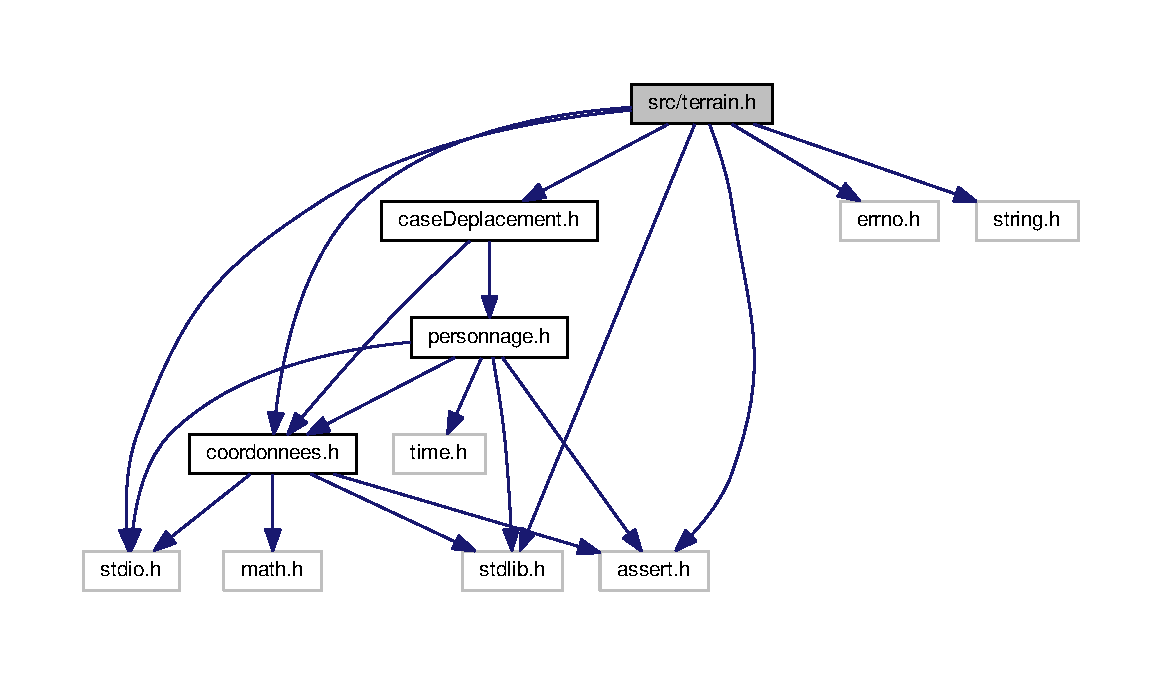
\includegraphics[width=350pt]{terrain_8h__incl}
\end{center}
\end{figure}
Ce graphe montre quels fichiers incluent directement ou indirectement ce fichier \+:
\nopagebreak
\begin{figure}[H]
\begin{center}
\leavevmode
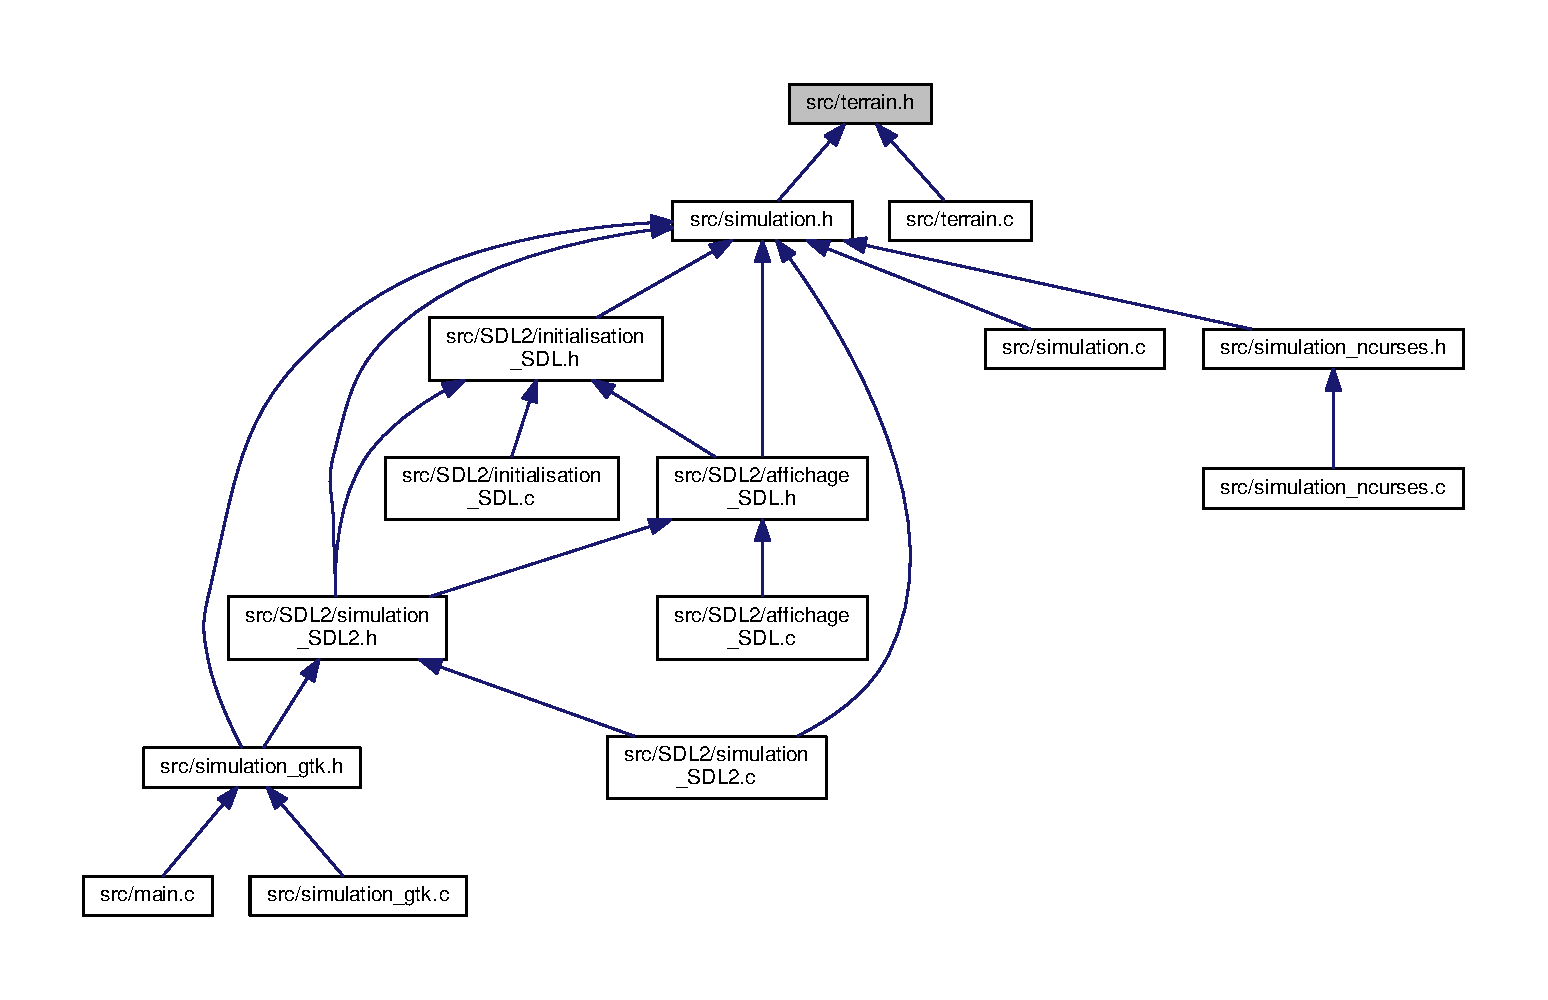
\includegraphics[width=350pt]{terrain_8h__dep__incl}
\end{center}
\end{figure}
\subsection*{Classes}
\begin{DoxyCompactItemize}
\item 
struct \hyperlink{structMTerrain}{M\+Terrain}
\begin{DoxyCompactList}\small\item\em Structure definissant un terrain et ses dimensions. \end{DoxyCompactList}\end{DoxyCompactItemize}
\subsection*{Macros}
\begin{DoxyCompactItemize}
\item 
\#define \hyperlink{terrain_8h_a5f41c70ea486e890717560da2605f309}{M\+A\+X\+\_\+\+C\+H\+A\+R\+\_\+\+N\+O\+M\+\_\+\+T\+E\+R\+R\+A\+IN}~500
\item 
\#define \hyperlink{terrain_8h_ad0ccb6c798f58235d0123be6ccb5e2b3}{M\+A\+X\+\_\+\+T\+A\+I\+L\+L\+E\+\_\+\+XY}~500
\end{DoxyCompactItemize}
\subsection*{Définitions de type}
\begin{DoxyCompactItemize}
\item 
typedef struct \hyperlink{structMTerrain}{M\+Terrain} \hyperlink{terrain_8h_a11bbfdc6f8212f3246205cc0e7134136}{Terrain}
\end{DoxyCompactItemize}
\subsection*{Fonctions}
\begin{DoxyCompactItemize}
\item 
void \hyperlink{terrain_8h_aa4dcb232d424b858d3f01f4951d411d4}{set\+Dim\+\_\+terr} (int x, int y, \hyperlink{terrain_8h_a11bbfdc6f8212f3246205cc0e7134136}{Terrain} $\ast$p\+Terrain)
\begin{DoxyCompactList}\small\item\em Edition de X et de Y dans la structure. \end{DoxyCompactList}\item 
void \hyperlink{terrain_8h_a80e61da510c086c125dd51ae23c518ff}{set\+Nom\+Terrain\+\_\+terr} (char nom\mbox{[}\hyperlink{terrain_8h_a5f41c70ea486e890717560da2605f309}{M\+A\+X\+\_\+\+C\+H\+A\+R\+\_\+\+N\+O\+M\+\_\+\+T\+E\+R\+R\+A\+IN}\mbox{]}, \hyperlink{terrain_8h_a11bbfdc6f8212f3246205cc0e7134136}{Terrain} $\ast$p\+Terrain)
\begin{DoxyCompactList}\small\item\em Edition du nom du terrain dans sa structure. \end{DoxyCompactList}\item 
void \hyperlink{terrain_8h_ad15a1365737240775ff8425378834fd6}{set\+Grille\+By\+X\+Y\+\_\+terr} (int x, int y, \hyperlink{terrain_8h_a11bbfdc6f8212f3246205cc0e7134136}{Terrain} $\ast$p\+Terrain, \hyperlink{caseDeplacement_8h_aeab4f22b99f0db8b549dab4e46e3ead4}{case\+Deplacement} $\ast$case\+Dep)
\begin{DoxyCompactList}\small\item\em Edition du type de la grille du terrain au coordonnées X/Y. \end{DoxyCompactList}\item 
int \hyperlink{terrain_8h_a09bd83bff226b5e25af2e9dfb160260c}{get\+Dim\+X\+\_\+terr} (\hyperlink{terrain_8h_a11bbfdc6f8212f3246205cc0e7134136}{Terrain} $\ast$p\+Terrain)
\begin{DoxyCompactList}\small\item\em Recupère la dimension en X de la structure Terrain. \end{DoxyCompactList}\item 
int \hyperlink{terrain_8h_a1fd39032dab5b6e3556883315a7868c5}{get\+Dim\+Y\+\_\+terr} (\hyperlink{terrain_8h_a11bbfdc6f8212f3246205cc0e7134136}{Terrain} $\ast$p\+Terrain)
\begin{DoxyCompactList}\small\item\em Recupère la dimension en Y de la structure Terrain. \end{DoxyCompactList}\item 
char $\ast$ \hyperlink{terrain_8h_aa2d2d29116636980d1b3f9f0a7a85ae0}{get\+Nom\+Terrain\+\_\+terr} (\hyperlink{terrain_8h_a11bbfdc6f8212f3246205cc0e7134136}{Terrain} $\ast$p\+Terrain)
\begin{DoxyCompactList}\small\item\em Recupère le nom de la structure Terrain. \end{DoxyCompactList}\item 
\hyperlink{caseDeplacement_8h_aeab4f22b99f0db8b549dab4e46e3ead4}{case\+Deplacement} $\ast$ \hyperlink{terrain_8h_a3b01a560ba891070ee62880f2739ea5b}{get\+Grille\+By\+X\+Y\+\_\+terr} (int x, int y, \hyperlink{terrain_8h_a11bbfdc6f8212f3246205cc0e7134136}{Terrain} $\ast$p\+Terrain)
\begin{DoxyCompactList}\small\item\em Recupere la case de deplacement de la grille au point X/Y. \end{DoxyCompactList}\item 
\hyperlink{caseDeplacement_8h_aeab4f22b99f0db8b549dab4e46e3ead4}{case\+Deplacement} $\ast$ \hyperlink{terrain_8h_a304eca02b8b49808ec4f456372fed6ff}{get\+Grille\+By\+Coord\+\_\+terr} (\hyperlink{coordonnees_8h_a79929cdfee7bd985a5e4e25276bb3ba9}{Coordonnees} $\ast$p\+Coord, \hyperlink{terrain_8h_a11bbfdc6f8212f3246205cc0e7134136}{Terrain} $\ast$p\+Terrain)
\begin{DoxyCompactList}\small\item\em Recupere la case de deplacement de la grille au coordonnées données. \end{DoxyCompactList}\item 
void \hyperlink{terrain_8h_a97c9cc766e38342e3425653e89b6f46c}{set\+Grille\+By\+Coord\+\_\+terr} (\hyperlink{coordonnees_8h_a79929cdfee7bd985a5e4e25276bb3ba9}{Coordonnees} $\ast$coord, \hyperlink{terrain_8h_a11bbfdc6f8212f3246205cc0e7134136}{Terrain} $\ast$p\+Terrain, \hyperlink{caseDeplacement_8h_aeab4f22b99f0db8b549dab4e46e3ead4}{case\+Deplacement} $\ast$case\+Dep)
\begin{DoxyCompactList}\small\item\em Change la case de deplacement de la grille au coordonnées données. \end{DoxyCompactList}\item 
\hyperlink{personnage_8h_abd5c92a453bbf273f753b3f5b99da9e7}{Perso} $\ast$ \hyperlink{terrain_8h_ae5f55773094ee4c234974d40b3287856}{cree\+Perso\+Terrain\+Rand} (\hyperlink{terrain_8h_a11bbfdc6f8212f3246205cc0e7134136}{Terrain} $\ast$p\+Terrain, enum \hyperlink{personnage_8h_a3f6a2951aa3d5d428dd6d61e74db0d75}{type\+Perso} type, int id\+Perso)
\item 
\hyperlink{caseDeplacement_8h_aeab4f22b99f0db8b549dab4e46e3ead4}{case\+Deplacement} $\ast$ \hyperlink{terrain_8h_af1ce19edb047ad98f13eb599869cc462}{get\+Case\+Bas\+By\+Coord} (\hyperlink{coordonnees_8h_a79929cdfee7bd985a5e4e25276bb3ba9}{Coordonnees} $\ast$coord, \hyperlink{terrain_8h_a11bbfdc6f8212f3246205cc0e7134136}{Terrain} $\ast$p\+Terrain)
\begin{DoxyCompactList}\small\item\em Recupere la case de deplacement de la grille en dessous des coordonée. \end{DoxyCompactList}\item 
\hyperlink{caseDeplacement_8h_aeab4f22b99f0db8b549dab4e46e3ead4}{case\+Deplacement} $\ast$ \hyperlink{terrain_8h_a7fe6b65294f394be319ead817fd6ec1e}{get\+Case\+Haut\+By\+Coord} (\hyperlink{coordonnees_8h_a79929cdfee7bd985a5e4e25276bb3ba9}{Coordonnees} $\ast$coord, \hyperlink{terrain_8h_a11bbfdc6f8212f3246205cc0e7134136}{Terrain} $\ast$p\+Terrain)
\begin{DoxyCompactList}\small\item\em Recupere la case de deplacement de la grille en haut des coordonée. \end{DoxyCompactList}\item 
\hyperlink{caseDeplacement_8h_aeab4f22b99f0db8b549dab4e46e3ead4}{case\+Deplacement} $\ast$ \hyperlink{terrain_8h_ac71d16722a67e2a956f88e60e445efe6}{get\+Case\+Gauche\+By\+Coord} (\hyperlink{coordonnees_8h_a79929cdfee7bd985a5e4e25276bb3ba9}{Coordonnees} $\ast$coord, \hyperlink{terrain_8h_a11bbfdc6f8212f3246205cc0e7134136}{Terrain} $\ast$p\+Terrain)
\begin{DoxyCompactList}\small\item\em Recupere la case de deplacement de la grille a gauche des coordonée. \end{DoxyCompactList}\item 
\hyperlink{caseDeplacement_8h_aeab4f22b99f0db8b549dab4e46e3ead4}{case\+Deplacement} $\ast$ \hyperlink{terrain_8h_a454f9cef12a6b3be9691dff9ee195125}{get\+Case\+Droite\+By\+Coord} (\hyperlink{coordonnees_8h_a79929cdfee7bd985a5e4e25276bb3ba9}{Coordonnees} $\ast$coord, \hyperlink{terrain_8h_a11bbfdc6f8212f3246205cc0e7134136}{Terrain} $\ast$p\+Terrain)
\begin{DoxyCompactList}\small\item\em Recupere la case de deplacement de la grille a droite des coordonée. \end{DoxyCompactList}\item 
void \hyperlink{terrain_8h_a3983dae49e4000872233e7d83205a247}{terrain\+Init\+Grille\+\_\+terr} (\hyperlink{terrain_8h_a11bbfdc6f8212f3246205cc0e7134136}{Terrain} $\ast$p\+Terrain)
\begin{DoxyCompactList}\small\item\em Initialise la grille d\textquotesingle{}un terrain. \end{DoxyCompactList}\item 
\hyperlink{terrain_8h_a11bbfdc6f8212f3246205cc0e7134136}{Terrain} $\ast$ \hyperlink{terrain_8h_a18be630674285fc320507f21282be35f}{terrain\+Creer\+\_\+terr} (int dimX, int dimY, char nom\+Terrain\mbox{[}\hyperlink{terrain_8h_a5f41c70ea486e890717560da2605f309}{M\+A\+X\+\_\+\+C\+H\+A\+R\+\_\+\+N\+O\+M\+\_\+\+T\+E\+R\+R\+A\+IN}\mbox{]})
\begin{DoxyCompactList}\small\item\em Creer un terrain avec les dimension et le nom choisi et initialise sa grille en appelant Terrain\+Init\+Grille. \end{DoxyCompactList}\item 
void \hyperlink{terrain_8h_adcec4a15a3bf0455ad742bdcd940f2cb}{testament\+Terrain\+\_\+terr} (\hyperlink{terrain_8h_a11bbfdc6f8212f3246205cc0e7134136}{Terrain} $\ast$p\+Terrain)
\begin{DoxyCompactList}\small\item\em Libere la mémoire occupé par un terrain. \end{DoxyCompactList}\item 
char \hyperlink{terrain_8h_a97c090e1c8063d66314f3be8b159e2cd}{est\+Dans\+Terrain\+\_\+terr} (\hyperlink{terrain_8h_a11bbfdc6f8212f3246205cc0e7134136}{Terrain} $\ast$p\+Terrain, \hyperlink{coordonnees_8h_a79929cdfee7bd985a5e4e25276bb3ba9}{Coordonnees} $\ast$p\+Coord)
\begin{DoxyCompactList}\small\item\em Verifie si des coordonnées appartiennent au terrain. \end{DoxyCompactList}\item 
char \hyperlink{terrain_8h_a9fba0242ab21d6632a379cd00ee20f0e}{verif\+Deplacement\+Haut\+\_\+perso} (\hyperlink{personnage_8h_abd5c92a453bbf273f753b3f5b99da9e7}{Perso} $\ast$p\+Perso, \hyperlink{terrain_8h_a11bbfdc6f8212f3246205cc0e7134136}{Terrain} $\ast$p\+Terrain)
\begin{DoxyCompactList}\small\item\em Verifie si le personnage peut aller en haut. \end{DoxyCompactList}\item 
char \hyperlink{terrain_8h_a8d3c2c01aa89e785014ad2209d990c0a}{verif\+Deplacement\+Bas\+\_\+perso} (\hyperlink{personnage_8h_abd5c92a453bbf273f753b3f5b99da9e7}{Perso} $\ast$p\+Perso, \hyperlink{terrain_8h_a11bbfdc6f8212f3246205cc0e7134136}{Terrain} $\ast$p\+Terrain)
\begin{DoxyCompactList}\small\item\em Verifie si le personnage peut aller en bas. \end{DoxyCompactList}\item 
char \hyperlink{terrain_8h_ad8a0578b05cf7d184a2f7c69465cefea}{verif\+Deplacement\+Gauche\+\_\+perso} (\hyperlink{personnage_8h_abd5c92a453bbf273f753b3f5b99da9e7}{Perso} $\ast$p\+Perso, \hyperlink{terrain_8h_a11bbfdc6f8212f3246205cc0e7134136}{Terrain} $\ast$p\+Terrain)
\begin{DoxyCompactList}\small\item\em Verifie si le personnage peut aller a gauche. \end{DoxyCompactList}\item 
char \hyperlink{terrain_8h_a0e34d630de41377283db24f865009ce7}{verif\+Deplacement\+Droite\+\_\+perso} (\hyperlink{personnage_8h_abd5c92a453bbf273f753b3f5b99da9e7}{Perso} $\ast$p\+Perso, \hyperlink{terrain_8h_a11bbfdc6f8212f3246205cc0e7134136}{Terrain} $\ast$p\+Terrain)
\begin{DoxyCompactList}\small\item\em Verifie si le personnage peut aller a droite. \end{DoxyCompactList}\item 
char \hyperlink{terrain_8h_ae09dc2657a465436713dc79a500fbbfd}{deplacement\+Haut\+\_\+perso} (\hyperlink{personnage_8h_abd5c92a453bbf273f753b3f5b99da9e7}{Perso} $\ast$p\+Perso, \hyperlink{terrain_8h_a11bbfdc6f8212f3246205cc0e7134136}{Terrain} $\ast$p\+Terrain)
\begin{DoxyCompactList}\small\item\em Deplace le personnage vers le haut (test avant qu\textquotesingle{}il peut etre deplacé dans ce sens) \end{DoxyCompactList}\item 
char \hyperlink{terrain_8h_a124dcf1c540a5e9f8987153c5629777b}{deplacement\+Bas\+\_\+perso} (\hyperlink{personnage_8h_abd5c92a453bbf273f753b3f5b99da9e7}{Perso} $\ast$p\+Perso, \hyperlink{terrain_8h_a11bbfdc6f8212f3246205cc0e7134136}{Terrain} $\ast$p\+Terrain)
\begin{DoxyCompactList}\small\item\em Deplace le personnage vers le bas (test avant qu\textquotesingle{}il peut etre deplacé dans ce sens) \end{DoxyCompactList}\item 
char \hyperlink{terrain_8h_a8c6c0b998f096f10a0ccad25a136b465}{deplacement\+Gauche\+\_\+perso} (\hyperlink{personnage_8h_abd5c92a453bbf273f753b3f5b99da9e7}{Perso} $\ast$p\+Perso, \hyperlink{terrain_8h_a11bbfdc6f8212f3246205cc0e7134136}{Terrain} $\ast$p\+Terrain)
\begin{DoxyCompactList}\small\item\em Deplace le personnage vers la gauche (test avant qu\textquotesingle{}il peut etre deplacé dans ce sens) \end{DoxyCompactList}\item 
char \hyperlink{terrain_8h_a385bedef7127b250811ce7f0218c66e3}{deplacement\+Droite\+\_\+perso} (\hyperlink{personnage_8h_abd5c92a453bbf273f753b3f5b99da9e7}{Perso} $\ast$p\+Perso, \hyperlink{terrain_8h_a11bbfdc6f8212f3246205cc0e7134136}{Terrain} $\ast$p\+Terrain)
\begin{DoxyCompactList}\small\item\em Deplace le personnage vers la droite (test avant qu\textquotesingle{}il peut etre deplacé dans ce sens) \end{DoxyCompactList}\item 
char \hyperlink{terrain_8h_a50e099874470bb6e68cbd44c68807aa5}{deplacement\+Aleatoire\+\_\+perso} (\hyperlink{personnage_8h_abd5c92a453bbf273f753b3f5b99da9e7}{Perso} $\ast$p\+Perso, \hyperlink{terrain_8h_a11bbfdc6f8212f3246205cc0e7134136}{Terrain} $\ast$p\+Terrain)
\begin{DoxyCompactList}\small\item\em Deplace le personnage dans une direction aléatoire (test avant qu\textquotesingle{}il peut etre deplacé dans ce sens) \end{DoxyCompactList}\item 
\hyperlink{personnage_8h_abd5c92a453bbf273f753b3f5b99da9e7}{Perso} $\ast$ \hyperlink{terrain_8h_aef0f8b09c8459770f8901c7f4bc93b6d}{zombie\+Contamine\+Humain} (\hyperlink{personnage_8h_abd5c92a453bbf273f753b3f5b99da9e7}{Perso} $\ast$p\+Zombie, \hyperlink{terrain_8h_a11bbfdc6f8212f3246205cc0e7134136}{Terrain} $\ast$p\+Terrain)
\item 
\hyperlink{personnage_8h_abd5c92a453bbf273f753b3f5b99da9e7}{Perso} $\ast$ \hyperlink{terrain_8h_ad4312194338f3849221a0ae93372b974}{policier\+Tue\+Zombie} (\hyperlink{personnage_8h_abd5c92a453bbf273f753b3f5b99da9e7}{Perso} $\ast$p\+Policier, \hyperlink{terrain_8h_a11bbfdc6f8212f3246205cc0e7134136}{Terrain} $\ast$p\+Terrain)
\item 
char \hyperlink{terrain_8h_a001f60dfb98bf19a3868269a3a8d4128}{zombie\+En\+Haut} (\hyperlink{terrain_8h_a11bbfdc6f8212f3246205cc0e7134136}{Terrain} $\ast$p\+Terrain, \hyperlink{coordonnees_8h_a79929cdfee7bd985a5e4e25276bb3ba9}{Coordonnees} $\ast$coord\+Zombie)
\begin{DoxyCompactList}\small\item\em Regarde si un zombie se trouve sur la se situant (lire libelé de la fonction) des coordonnées. \end{DoxyCompactList}\item 
char \hyperlink{terrain_8h_ad4328106195808c5a5a40e869ad7a580}{zombie\+En\+Bas} (\hyperlink{terrain_8h_a11bbfdc6f8212f3246205cc0e7134136}{Terrain} $\ast$p\+Terrain, \hyperlink{coordonnees_8h_a79929cdfee7bd985a5e4e25276bb3ba9}{Coordonnees} $\ast$coord\+Zombie)
\begin{DoxyCompactList}\small\item\em Regarde si un zombie se trouve sur la se situant (lire libelé de la fonction) des coordonnées. \end{DoxyCompactList}\item 
char \hyperlink{terrain_8h_af6ccfdc77c33d99a1ae6807aa7c8da8a}{zombie\+A\+Gauche} (\hyperlink{terrain_8h_a11bbfdc6f8212f3246205cc0e7134136}{Terrain} $\ast$p\+Terrain, \hyperlink{coordonnees_8h_a79929cdfee7bd985a5e4e25276bb3ba9}{Coordonnees} $\ast$coord\+Zombie)
\begin{DoxyCompactList}\small\item\em Regarde si un zombie se trouve sur la se situant (lire libelé de la fonction) des coordonnées. \end{DoxyCompactList}\item 
char \hyperlink{terrain_8h_a26dc558207a13a9ee19f2c78d06bf807}{zombie\+A\+Droite} (\hyperlink{terrain_8h_a11bbfdc6f8212f3246205cc0e7134136}{Terrain} $\ast$p\+Terrain, \hyperlink{coordonnees_8h_a79929cdfee7bd985a5e4e25276bb3ba9}{Coordonnees} $\ast$coord\+Zombie)
\begin{DoxyCompactList}\small\item\em Regarde si un zombie se trouve sur la se situant (lire libelé de la fonction) des coordonnées. \end{DoxyCompactList}\item 
char \hyperlink{terrain_8h_ad15a715cc6d4d24dbd1f1b0c5c724c41}{zombie\+En2\+Haut} (\hyperlink{terrain_8h_a11bbfdc6f8212f3246205cc0e7134136}{Terrain} $\ast$p\+Terrain, \hyperlink{coordonnees_8h_a79929cdfee7bd985a5e4e25276bb3ba9}{Coordonnees} $\ast$coord\+Zombie)
\begin{DoxyCompactList}\small\item\em Regarde si un zombie se trouve sur la se situant (lire libelé de la fonction) des coordonnées. \end{DoxyCompactList}\item 
char \hyperlink{terrain_8h_aac1c61b2b5fb5333e2c71072597fe646}{zombie\+En2\+Bas} (\hyperlink{terrain_8h_a11bbfdc6f8212f3246205cc0e7134136}{Terrain} $\ast$p\+Terrain, \hyperlink{coordonnees_8h_a79929cdfee7bd985a5e4e25276bb3ba9}{Coordonnees} $\ast$coord\+Zombie)
\begin{DoxyCompactList}\small\item\em Regarde si un zombie se trouve sur la se situant (lire libelé de la fonction) des coordonnées. \end{DoxyCompactList}\item 
char \hyperlink{terrain_8h_a789481a25a7883fa13a345b5cc86b618}{zombie\+A2\+Gauche} (\hyperlink{terrain_8h_a11bbfdc6f8212f3246205cc0e7134136}{Terrain} $\ast$p\+Terrain, \hyperlink{coordonnees_8h_a79929cdfee7bd985a5e4e25276bb3ba9}{Coordonnees} $\ast$coord\+Zombie)
\begin{DoxyCompactList}\small\item\em Regarde si un zombie se trouve sur la se situant (lire libelé de la fonction) des coordonnées. \end{DoxyCompactList}\item 
char \hyperlink{terrain_8h_a97157bb01d1c0e7eed68d43459410dfc}{zombie\+A2\+Droite} (\hyperlink{terrain_8h_a11bbfdc6f8212f3246205cc0e7134136}{Terrain} $\ast$p\+Terrain, \hyperlink{coordonnees_8h_a79929cdfee7bd985a5e4e25276bb3ba9}{Coordonnees} $\ast$coord\+Zombie)
\begin{DoxyCompactList}\small\item\em Regarde si un zombie se trouve sur la se situant (lire libelé de la fonction) des coordonnées. \end{DoxyCompactList}\item 
char \hyperlink{terrain_8h_ac83836d426c8c3f520114923a555a9bb}{zombie\+HD} (\hyperlink{terrain_8h_a11bbfdc6f8212f3246205cc0e7134136}{Terrain} $\ast$p\+Terrain, \hyperlink{coordonnees_8h_a79929cdfee7bd985a5e4e25276bb3ba9}{Coordonnees} $\ast$coord\+Zombie)
\begin{DoxyCompactList}\small\item\em Regarde si un zombie se trouve sur la se situant (lire libelé de la fonction) des coordonnées. \end{DoxyCompactList}\item 
char \hyperlink{terrain_8h_abba9a396650e8815b0a0d8c093fbc352}{zombie\+BD} (\hyperlink{terrain_8h_a11bbfdc6f8212f3246205cc0e7134136}{Terrain} $\ast$p\+Terrain, \hyperlink{coordonnees_8h_a79929cdfee7bd985a5e4e25276bb3ba9}{Coordonnees} $\ast$coord\+Zombie)
\begin{DoxyCompactList}\small\item\em Regarde si un zombie se trouve sur la se situant (lire libelé de la fonction) des coordonnées. \end{DoxyCompactList}\item 
char \hyperlink{terrain_8h_adc99a25c35fcd27644a47f14129e0278}{zombie\+BG} (\hyperlink{terrain_8h_a11bbfdc6f8212f3246205cc0e7134136}{Terrain} $\ast$p\+Terrain, \hyperlink{coordonnees_8h_a79929cdfee7bd985a5e4e25276bb3ba9}{Coordonnees} $\ast$coord\+Zombie)
\begin{DoxyCompactList}\small\item\em Regarde si un zombie se trouve sur la se situant (lire libelé de la fonction) des coordonnées. \end{DoxyCompactList}\item 
char \hyperlink{terrain_8h_a620533e1f0789251d879b67d9cef829e}{zombie\+HG} (\hyperlink{terrain_8h_a11bbfdc6f8212f3246205cc0e7134136}{Terrain} $\ast$p\+Terrain, \hyperlink{coordonnees_8h_a79929cdfee7bd985a5e4e25276bb3ba9}{Coordonnees} $\ast$coord\+Zombie)
\begin{DoxyCompactList}\small\item\em Regarde si un zombie se trouve sur la se situant (lire libelé de la fonction) des coordonnées. \end{DoxyCompactList}\item 
char \hyperlink{terrain_8h_ae6548343b2ab3ffd042731aeee925261}{humain\+En\+Haut} (\hyperlink{terrain_8h_a11bbfdc6f8212f3246205cc0e7134136}{Terrain} $\ast$p\+Terrain, \hyperlink{coordonnees_8h_a79929cdfee7bd985a5e4e25276bb3ba9}{Coordonnees} $\ast$coord\+Zombie)
\begin{DoxyCompactList}\small\item\em Verifie si le personnage en haut est un humain. \end{DoxyCompactList}\item 
char \hyperlink{terrain_8h_a50df7bb2b9b06787410c5c3c18c26c7e}{humain\+En\+Bas} (\hyperlink{terrain_8h_a11bbfdc6f8212f3246205cc0e7134136}{Terrain} $\ast$p\+Terrain, \hyperlink{coordonnees_8h_a79929cdfee7bd985a5e4e25276bb3ba9}{Coordonnees} $\ast$coord\+Zombie)
\begin{DoxyCompactList}\small\item\em Verifie si le personnage en bas est un humain. \end{DoxyCompactList}\item 
char \hyperlink{terrain_8h_aa81fd0c9d275c8f8feb23f1400f43e43}{humain\+A\+Gauche} (\hyperlink{terrain_8h_a11bbfdc6f8212f3246205cc0e7134136}{Terrain} $\ast$p\+Terrain, \hyperlink{coordonnees_8h_a79929cdfee7bd985a5e4e25276bb3ba9}{Coordonnees} $\ast$coord\+Zombie)
\begin{DoxyCompactList}\small\item\em Verifie si le personnage a gauche est un humain. \end{DoxyCompactList}\item 
char \hyperlink{terrain_8h_a5f78f92ecac28d78ffd95ba3e04b272d}{humain\+A\+Droite} (\hyperlink{terrain_8h_a11bbfdc6f8212f3246205cc0e7134136}{Terrain} $\ast$p\+Terrain, \hyperlink{coordonnees_8h_a79929cdfee7bd985a5e4e25276bb3ba9}{Coordonnees} $\ast$coord\+Zombie)
\begin{DoxyCompactList}\small\item\em Verifie si le personnage a droite est un humain. \end{DoxyCompactList}\item 
void \hyperlink{terrain_8h_aba7a3bbec5c24c999958be6699d8fc11}{afficher\+Grille\+Console} (\hyperlink{terrain_8h_a11bbfdc6f8212f3246205cc0e7134136}{Terrain} $\ast$p\+Terrain)
\begin{DoxyCompactList}\small\item\em Affiche la grille dans la console avec des caractère pour représenter les personnages et murs. \end{DoxyCompactList}\item 
void \hyperlink{terrain_8h_ae74ede311bdc4b21f792dac31ba78834}{terrain\+Creer\+Fichier\+\_\+terr} (\hyperlink{terrain_8h_a11bbfdc6f8212f3246205cc0e7134136}{Terrain} $\ast$p\+Terrain, char $\ast$chemin\+Fichier)
\begin{DoxyCompactList}\small\item\em Créer un fichier terrain à partir du pointeur vers terrain. \end{DoxyCompactList}\item 
\hyperlink{terrain_8h_a11bbfdc6f8212f3246205cc0e7134136}{Terrain} $\ast$ \hyperlink{terrain_8h_ab263e5c5999c16af432acbb69e777a67}{terrain\+Lire\+Fichier\+\_\+terr} (char $\ast$chemin\+Fichier)
\begin{DoxyCompactList}\small\item\em Lit le fichier terrain de nom spécifié et le retourne par un pointeur. \end{DoxyCompactList}\item 
void \hyperlink{terrain_8h_a1ec738cacf8012e6e62410e31cd56d62}{afficher\+Champs} (\hyperlink{terrain_8h_a11bbfdc6f8212f3246205cc0e7134136}{Terrain} $\ast$p\+Terrain)
\begin{DoxyCompactList}\small\item\em Affiche la grille des champs dans la console avec des caractère pour représenter les représenter. \end{DoxyCompactList}\item 
void \hyperlink{terrain_8h_aad20d9f641c2045b6556280495340013}{terrain\+Ajout\+Mur\+Tour} (\hyperlink{terrain_8h_a11bbfdc6f8212f3246205cc0e7134136}{Terrain} $\ast$p\+Terrain)
\begin{DoxyCompactList}\small\item\em Ajoute des mur sur les bord du terrain. \end{DoxyCompactList}\item 
void \hyperlink{terrain_8h_aa4fd8914490a8a95ff9e96de4b4cd6c4}{initialisation\+Marqueurs} (\hyperlink{terrain_8h_a11bbfdc6f8212f3246205cc0e7134136}{Terrain} $\ast$p\+Terrain)
\begin{DoxyCompactList}\small\item\em Initialisé la grille des champs à 0 avec des marqueurs. \end{DoxyCompactList}\item 
void \hyperlink{terrain_8h_af32214c124513367869c101ca6576bac}{propagation\+Champ} (enum \hyperlink{personnage_8h_a3f6a2951aa3d5d428dd6d61e74db0d75}{type\+Perso} type, int id\+Perso, \hyperlink{coordonnees_8h_a79929cdfee7bd985a5e4e25276bb3ba9}{Coordonnees} $\ast$coord\+Perso, \hyperlink{terrain_8h_a11bbfdc6f8212f3246205cc0e7134136}{Terrain} $\ast$p\+Terrain)
\item 
void \hyperlink{terrain_8h_ae671405a2cab0685307937720369b63f}{test\+Fonctions\+\_\+terr} ()
\begin{DoxyCompactList}\small\item\em Fonctoin de test des fonction du module terrain. \end{DoxyCompactList}\item 
void \hyperlink{terrain_8h_a5864b0a17c6c301ff1e2f574e3ae244c}{init\+Champs\+Terrain} (int nb\+Zombie, int nb\+Citoyens, int nb\+Policiers, \hyperlink{terrain_8h_a11bbfdc6f8212f3246205cc0e7134136}{Terrain} $\ast$p\+Terrain)
\end{DoxyCompactItemize}


\subsection{Description détaillée}
Définit les fonctions et les structures du terrain. 



\subsection{Documentation des macros}
\index{terrain.\+h@{terrain.\+h}!M\+A\+X\+\_\+\+C\+H\+A\+R\+\_\+\+N\+O\+M\+\_\+\+T\+E\+R\+R\+A\+IN@{M\+A\+X\+\_\+\+C\+H\+A\+R\+\_\+\+N\+O\+M\+\_\+\+T\+E\+R\+R\+A\+IN}}
\index{M\+A\+X\+\_\+\+C\+H\+A\+R\+\_\+\+N\+O\+M\+\_\+\+T\+E\+R\+R\+A\+IN@{M\+A\+X\+\_\+\+C\+H\+A\+R\+\_\+\+N\+O\+M\+\_\+\+T\+E\+R\+R\+A\+IN}!terrain.\+h@{terrain.\+h}}
\subsubsection[{\texorpdfstring{M\+A\+X\+\_\+\+C\+H\+A\+R\+\_\+\+N\+O\+M\+\_\+\+T\+E\+R\+R\+A\+IN}{MAX_CHAR_NOM_TERRAIN}}]{\setlength{\rightskip}{0pt plus 5cm}\#define M\+A\+X\+\_\+\+C\+H\+A\+R\+\_\+\+N\+O\+M\+\_\+\+T\+E\+R\+R\+A\+IN~500}\hypertarget{terrain_8h_a5f41c70ea486e890717560da2605f309}{}\label{terrain_8h_a5f41c70ea486e890717560da2605f309}
\index{terrain.\+h@{terrain.\+h}!M\+A\+X\+\_\+\+T\+A\+I\+L\+L\+E\+\_\+\+XY@{M\+A\+X\+\_\+\+T\+A\+I\+L\+L\+E\+\_\+\+XY}}
\index{M\+A\+X\+\_\+\+T\+A\+I\+L\+L\+E\+\_\+\+XY@{M\+A\+X\+\_\+\+T\+A\+I\+L\+L\+E\+\_\+\+XY}!terrain.\+h@{terrain.\+h}}
\subsubsection[{\texorpdfstring{M\+A\+X\+\_\+\+T\+A\+I\+L\+L\+E\+\_\+\+XY}{MAX_TAILLE_XY}}]{\setlength{\rightskip}{0pt plus 5cm}\#define M\+A\+X\+\_\+\+T\+A\+I\+L\+L\+E\+\_\+\+XY~500}\hypertarget{terrain_8h_ad0ccb6c798f58235d0123be6ccb5e2b3}{}\label{terrain_8h_ad0ccb6c798f58235d0123be6ccb5e2b3}


\subsection{Documentation des définitions de type}
\index{terrain.\+h@{terrain.\+h}!Terrain@{Terrain}}
\index{Terrain@{Terrain}!terrain.\+h@{terrain.\+h}}
\subsubsection[{\texorpdfstring{Terrain}{Terrain}}]{\setlength{\rightskip}{0pt plus 5cm}typedef struct {\bf M\+Terrain}  {\bf Terrain}}\hypertarget{terrain_8h_a11bbfdc6f8212f3246205cc0e7134136}{}\label{terrain_8h_a11bbfdc6f8212f3246205cc0e7134136}


\subsection{Documentation des fonctions}
\index{terrain.\+h@{terrain.\+h}!afficher\+Champs@{afficher\+Champs}}
\index{afficher\+Champs@{afficher\+Champs}!terrain.\+h@{terrain.\+h}}
\subsubsection[{\texorpdfstring{afficher\+Champs(\+Terrain $\ast$p\+Terrain)}{afficherChamps(Terrain *pTerrain)}}]{\setlength{\rightskip}{0pt plus 5cm}void afficher\+Champs (
\begin{DoxyParamCaption}
\item[{{\bf Terrain} $\ast$}]{p\+Terrain}
\end{DoxyParamCaption}
)}\hypertarget{terrain_8h_a1ec738cacf8012e6e62410e31cd56d62}{}\label{terrain_8h_a1ec738cacf8012e6e62410e31cd56d62}


Affiche la grille des champs dans la console avec des caractère pour représenter les représenter. 

\index{terrain.\+h@{terrain.\+h}!afficher\+Grille\+Console@{afficher\+Grille\+Console}}
\index{afficher\+Grille\+Console@{afficher\+Grille\+Console}!terrain.\+h@{terrain.\+h}}
\subsubsection[{\texorpdfstring{afficher\+Grille\+Console(\+Terrain $\ast$p\+Terrain)}{afficherGrilleConsole(Terrain *pTerrain)}}]{\setlength{\rightskip}{0pt plus 5cm}void afficher\+Grille\+Console (
\begin{DoxyParamCaption}
\item[{{\bf Terrain} $\ast$}]{p\+Terrain}
\end{DoxyParamCaption}
)}\hypertarget{terrain_8h_aba7a3bbec5c24c999958be6699d8fc11}{}\label{terrain_8h_aba7a3bbec5c24c999958be6699d8fc11}


Affiche la grille dans la console avec des caractère pour représenter les personnages et murs. 

\index{terrain.\+h@{terrain.\+h}!cree\+Perso\+Terrain\+Rand@{cree\+Perso\+Terrain\+Rand}}
\index{cree\+Perso\+Terrain\+Rand@{cree\+Perso\+Terrain\+Rand}!terrain.\+h@{terrain.\+h}}
\subsubsection[{\texorpdfstring{cree\+Perso\+Terrain\+Rand(\+Terrain $\ast$p\+Terrain, enum type\+Perso type, int id\+Perso)}{creePersoTerrainRand(Terrain *pTerrain, enum typePerso type, int idPerso)}}]{\setlength{\rightskip}{0pt plus 5cm}{\bf Perso}$\ast$ cree\+Perso\+Terrain\+Rand (
\begin{DoxyParamCaption}
\item[{{\bf Terrain} $\ast$}]{p\+Terrain, }
\item[{enum {\bf type\+Perso}}]{type, }
\item[{int}]{id\+Perso}
\end{DoxyParamCaption}
)}\hypertarget{terrain_8h_ae5f55773094ee4c234974d40b3287856}{}\label{terrain_8h_ae5f55773094ee4c234974d40b3287856}
\index{terrain.\+h@{terrain.\+h}!deplacement\+Aleatoire\+\_\+perso@{deplacement\+Aleatoire\+\_\+perso}}
\index{deplacement\+Aleatoire\+\_\+perso@{deplacement\+Aleatoire\+\_\+perso}!terrain.\+h@{terrain.\+h}}
\subsubsection[{\texorpdfstring{deplacement\+Aleatoire\+\_\+perso(\+Perso $\ast$p\+Perso, Terrain $\ast$p\+Terrain)}{deplacementAleatoire_perso(Perso *pPerso, Terrain *pTerrain)}}]{\setlength{\rightskip}{0pt plus 5cm}char deplacement\+Aleatoire\+\_\+perso (
\begin{DoxyParamCaption}
\item[{{\bf Perso} $\ast$}]{p\+Perso, }
\item[{{\bf Terrain} $\ast$}]{p\+Terrain}
\end{DoxyParamCaption}
)}\hypertarget{terrain_8h_a50e099874470bb6e68cbd44c68807aa5}{}\label{terrain_8h_a50e099874470bb6e68cbd44c68807aa5}


Deplace le personnage dans une direction aléatoire (test avant qu\textquotesingle{}il peut etre deplacé dans ce sens) 


\begin{DoxyParams}{Paramètres}
{\em p\+Perso} & Pointeur vers le personnage dont les deplacement serront testé \\
\hline
{\em p\+Terrain} & Le terrain ou les coordonnées vont etre vérifiés \\
\hline
\end{DoxyParams}
\begin{DoxyReturn}{Renvoie}
1 si le personnage a été deplacé, 0 sinon, sous forme d\textquotesingle{}un caractere 
\end{DoxyReturn}
\index{terrain.\+h@{terrain.\+h}!deplacement\+Bas\+\_\+perso@{deplacement\+Bas\+\_\+perso}}
\index{deplacement\+Bas\+\_\+perso@{deplacement\+Bas\+\_\+perso}!terrain.\+h@{terrain.\+h}}
\subsubsection[{\texorpdfstring{deplacement\+Bas\+\_\+perso(\+Perso $\ast$p\+Perso, Terrain $\ast$p\+Terrain)}{deplacementBas_perso(Perso *pPerso, Terrain *pTerrain)}}]{\setlength{\rightskip}{0pt plus 5cm}char deplacement\+Bas\+\_\+perso (
\begin{DoxyParamCaption}
\item[{{\bf Perso} $\ast$}]{p\+Perso, }
\item[{{\bf Terrain} $\ast$}]{p\+Terrain}
\end{DoxyParamCaption}
)}\hypertarget{terrain_8h_a124dcf1c540a5e9f8987153c5629777b}{}\label{terrain_8h_a124dcf1c540a5e9f8987153c5629777b}


Deplace le personnage vers le bas (test avant qu\textquotesingle{}il peut etre deplacé dans ce sens) 


\begin{DoxyParams}{Paramètres}
{\em p\+Perso} & Pointeur vers le personnage dont les deplacement serront testé \\
\hline
{\em p\+Terrain} & Le terrain ou les coordonnées vont etre vérifiés \\
\hline
\end{DoxyParams}
\begin{DoxyReturn}{Renvoie}
1 si le personnage a été deplacé, 0 sinon, sous forme d\textquotesingle{}un caractere 
\end{DoxyReturn}
\index{terrain.\+h@{terrain.\+h}!deplacement\+Droite\+\_\+perso@{deplacement\+Droite\+\_\+perso}}
\index{deplacement\+Droite\+\_\+perso@{deplacement\+Droite\+\_\+perso}!terrain.\+h@{terrain.\+h}}
\subsubsection[{\texorpdfstring{deplacement\+Droite\+\_\+perso(\+Perso $\ast$p\+Perso, Terrain $\ast$p\+Terrain)}{deplacementDroite_perso(Perso *pPerso, Terrain *pTerrain)}}]{\setlength{\rightskip}{0pt plus 5cm}char deplacement\+Droite\+\_\+perso (
\begin{DoxyParamCaption}
\item[{{\bf Perso} $\ast$}]{p\+Perso, }
\item[{{\bf Terrain} $\ast$}]{p\+Terrain}
\end{DoxyParamCaption}
)}\hypertarget{terrain_8h_a385bedef7127b250811ce7f0218c66e3}{}\label{terrain_8h_a385bedef7127b250811ce7f0218c66e3}


Deplace le personnage vers la droite (test avant qu\textquotesingle{}il peut etre deplacé dans ce sens) 


\begin{DoxyParams}{Paramètres}
{\em p\+Perso} & Pointeur vers le personnage dont les deplacement serront testé \\
\hline
{\em p\+Terrain} & Le terrain ou les coordonnées vont etre vérifiés \\
\hline
\end{DoxyParams}
\begin{DoxyReturn}{Renvoie}
1 si le personnage a été deplacé, 0 sinon, sous forme d\textquotesingle{}un caractere 
\end{DoxyReturn}
\index{terrain.\+h@{terrain.\+h}!deplacement\+Gauche\+\_\+perso@{deplacement\+Gauche\+\_\+perso}}
\index{deplacement\+Gauche\+\_\+perso@{deplacement\+Gauche\+\_\+perso}!terrain.\+h@{terrain.\+h}}
\subsubsection[{\texorpdfstring{deplacement\+Gauche\+\_\+perso(\+Perso $\ast$p\+Perso, Terrain $\ast$p\+Terrain)}{deplacementGauche_perso(Perso *pPerso, Terrain *pTerrain)}}]{\setlength{\rightskip}{0pt plus 5cm}char deplacement\+Gauche\+\_\+perso (
\begin{DoxyParamCaption}
\item[{{\bf Perso} $\ast$}]{p\+Perso, }
\item[{{\bf Terrain} $\ast$}]{p\+Terrain}
\end{DoxyParamCaption}
)}\hypertarget{terrain_8h_a8c6c0b998f096f10a0ccad25a136b465}{}\label{terrain_8h_a8c6c0b998f096f10a0ccad25a136b465}


Deplace le personnage vers la gauche (test avant qu\textquotesingle{}il peut etre deplacé dans ce sens) 


\begin{DoxyParams}{Paramètres}
{\em p\+Perso} & Pointeur vers le personnage dont les deplacement serront testé \\
\hline
{\em p\+Terrain} & Le terrain ou les coordonnées vont etre vérifiés \\
\hline
\end{DoxyParams}
\begin{DoxyReturn}{Renvoie}
1 si le personnage a été deplacé, 0 sinon, sous forme d\textquotesingle{}un caractere 
\end{DoxyReturn}
\index{terrain.\+h@{terrain.\+h}!deplacement\+Haut\+\_\+perso@{deplacement\+Haut\+\_\+perso}}
\index{deplacement\+Haut\+\_\+perso@{deplacement\+Haut\+\_\+perso}!terrain.\+h@{terrain.\+h}}
\subsubsection[{\texorpdfstring{deplacement\+Haut\+\_\+perso(\+Perso $\ast$p\+Perso, Terrain $\ast$p\+Terrain)}{deplacementHaut_perso(Perso *pPerso, Terrain *pTerrain)}}]{\setlength{\rightskip}{0pt plus 5cm}char deplacement\+Haut\+\_\+perso (
\begin{DoxyParamCaption}
\item[{{\bf Perso} $\ast$}]{p\+Perso, }
\item[{{\bf Terrain} $\ast$}]{p\+Terrain}
\end{DoxyParamCaption}
)}\hypertarget{terrain_8h_ae09dc2657a465436713dc79a500fbbfd}{}\label{terrain_8h_ae09dc2657a465436713dc79a500fbbfd}


Deplace le personnage vers le haut (test avant qu\textquotesingle{}il peut etre deplacé dans ce sens) 


\begin{DoxyParams}{Paramètres}
{\em p\+Perso} & Pointeur vers le personnage dont les deplacement serront testé \\
\hline
{\em p\+Terrain} & Le terrain ou les coordonnées vont etre vérifiés \\
\hline
\end{DoxyParams}
\begin{DoxyReturn}{Renvoie}
1 si le personnage a été deplacé, 0 sinon, sous forme d\textquotesingle{}un caractere 
\end{DoxyReturn}
\index{terrain.\+h@{terrain.\+h}!est\+Dans\+Terrain\+\_\+terr@{est\+Dans\+Terrain\+\_\+terr}}
\index{est\+Dans\+Terrain\+\_\+terr@{est\+Dans\+Terrain\+\_\+terr}!terrain.\+h@{terrain.\+h}}
\subsubsection[{\texorpdfstring{est\+Dans\+Terrain\+\_\+terr(\+Terrain $\ast$p\+Terrain, Coordonnees $\ast$p\+Coord)}{estDansTerrain_terr(Terrain *pTerrain, Coordonnees *pCoord)}}]{\setlength{\rightskip}{0pt plus 5cm}char est\+Dans\+Terrain\+\_\+terr (
\begin{DoxyParamCaption}
\item[{{\bf Terrain} $\ast$}]{p\+Terrain, }
\item[{{\bf Coordonnees} $\ast$}]{p\+Coord}
\end{DoxyParamCaption}
)}\hypertarget{terrain_8h_a97c090e1c8063d66314f3be8b159e2cd}{}\label{terrain_8h_a97c090e1c8063d66314f3be8b159e2cd}


Verifie si des coordonnées appartiennent au terrain. 


\begin{DoxyParams}{Paramètres}
{\em p\+Terrain} & Le terrain ou les coordonnées vont etre vérifiés \\
\hline
{\em p\+Coord} & Les coordonnées a verifier \\
\hline
\end{DoxyParams}
\begin{DoxyReturn}{Renvoie}
1 si oui, 0 sinon, sous forme d\textquotesingle{}un caractere 
\end{DoxyReturn}
\index{terrain.\+h@{terrain.\+h}!get\+Case\+Bas\+By\+Coord@{get\+Case\+Bas\+By\+Coord}}
\index{get\+Case\+Bas\+By\+Coord@{get\+Case\+Bas\+By\+Coord}!terrain.\+h@{terrain.\+h}}
\subsubsection[{\texorpdfstring{get\+Case\+Bas\+By\+Coord(\+Coordonnees $\ast$coord, Terrain $\ast$p\+Terrain)}{getCaseBasByCoord(Coordonnees *coord, Terrain *pTerrain)}}]{\setlength{\rightskip}{0pt plus 5cm}{\bf case\+Deplacement}$\ast$ get\+Case\+Bas\+By\+Coord (
\begin{DoxyParamCaption}
\item[{{\bf Coordonnees} $\ast$}]{coord, }
\item[{{\bf Terrain} $\ast$}]{p\+Terrain}
\end{DoxyParamCaption}
)}\hypertarget{terrain_8h_af1ce19edb047ad98f13eb599869cc462}{}\label{terrain_8h_af1ce19edb047ad98f13eb599869cc462}


Recupere la case de deplacement de la grille en dessous des coordonée. 


\begin{DoxyParams}{Paramètres}
{\em coord} & Coordonnée ou aller recuperer \\
\hline
{\em p\+Terrain} & Pointeur sur la structure Terrain a editer \\
\hline
\end{DoxyParams}
\begin{DoxyReturn}{Renvoie}
Case de deplacement en dessous 
\end{DoxyReturn}
\index{terrain.\+h@{terrain.\+h}!get\+Case\+Droite\+By\+Coord@{get\+Case\+Droite\+By\+Coord}}
\index{get\+Case\+Droite\+By\+Coord@{get\+Case\+Droite\+By\+Coord}!terrain.\+h@{terrain.\+h}}
\subsubsection[{\texorpdfstring{get\+Case\+Droite\+By\+Coord(\+Coordonnees $\ast$coord, Terrain $\ast$p\+Terrain)}{getCaseDroiteByCoord(Coordonnees *coord, Terrain *pTerrain)}}]{\setlength{\rightskip}{0pt plus 5cm}{\bf case\+Deplacement}$\ast$ get\+Case\+Droite\+By\+Coord (
\begin{DoxyParamCaption}
\item[{{\bf Coordonnees} $\ast$}]{coord, }
\item[{{\bf Terrain} $\ast$}]{p\+Terrain}
\end{DoxyParamCaption}
)}\hypertarget{terrain_8h_a454f9cef12a6b3be9691dff9ee195125}{}\label{terrain_8h_a454f9cef12a6b3be9691dff9ee195125}


Recupere la case de deplacement de la grille a droite des coordonée. 


\begin{DoxyParams}{Paramètres}
{\em coord} & Coordonnée ou aller recuperer \\
\hline
{\em p\+Terrain} & Pointeur sur la structure Terrain a editer \\
\hline
\end{DoxyParams}
\begin{DoxyReturn}{Renvoie}
Case de deplacement a droite 
\end{DoxyReturn}
\index{terrain.\+h@{terrain.\+h}!get\+Case\+Gauche\+By\+Coord@{get\+Case\+Gauche\+By\+Coord}}
\index{get\+Case\+Gauche\+By\+Coord@{get\+Case\+Gauche\+By\+Coord}!terrain.\+h@{terrain.\+h}}
\subsubsection[{\texorpdfstring{get\+Case\+Gauche\+By\+Coord(\+Coordonnees $\ast$coord, Terrain $\ast$p\+Terrain)}{getCaseGaucheByCoord(Coordonnees *coord, Terrain *pTerrain)}}]{\setlength{\rightskip}{0pt plus 5cm}{\bf case\+Deplacement}$\ast$ get\+Case\+Gauche\+By\+Coord (
\begin{DoxyParamCaption}
\item[{{\bf Coordonnees} $\ast$}]{coord, }
\item[{{\bf Terrain} $\ast$}]{p\+Terrain}
\end{DoxyParamCaption}
)}\hypertarget{terrain_8h_ac71d16722a67e2a956f88e60e445efe6}{}\label{terrain_8h_ac71d16722a67e2a956f88e60e445efe6}


Recupere la case de deplacement de la grille a gauche des coordonée. 


\begin{DoxyParams}{Paramètres}
{\em coord} & Coordonnée ou aller recuperer \\
\hline
{\em p\+Terrain} & Pointeur sur la structure Terrain a editer \\
\hline
\end{DoxyParams}
\begin{DoxyReturn}{Renvoie}
Case de deplacement a gauche 
\end{DoxyReturn}
\index{terrain.\+h@{terrain.\+h}!get\+Case\+Haut\+By\+Coord@{get\+Case\+Haut\+By\+Coord}}
\index{get\+Case\+Haut\+By\+Coord@{get\+Case\+Haut\+By\+Coord}!terrain.\+h@{terrain.\+h}}
\subsubsection[{\texorpdfstring{get\+Case\+Haut\+By\+Coord(\+Coordonnees $\ast$coord, Terrain $\ast$p\+Terrain)}{getCaseHautByCoord(Coordonnees *coord, Terrain *pTerrain)}}]{\setlength{\rightskip}{0pt plus 5cm}{\bf case\+Deplacement}$\ast$ get\+Case\+Haut\+By\+Coord (
\begin{DoxyParamCaption}
\item[{{\bf Coordonnees} $\ast$}]{coord, }
\item[{{\bf Terrain} $\ast$}]{p\+Terrain}
\end{DoxyParamCaption}
)}\hypertarget{terrain_8h_a7fe6b65294f394be319ead817fd6ec1e}{}\label{terrain_8h_a7fe6b65294f394be319ead817fd6ec1e}


Recupere la case de deplacement de la grille en haut des coordonée. 


\begin{DoxyParams}{Paramètres}
{\em coord} & Coordonnée ou aller recuperer \\
\hline
{\em p\+Terrain} & Pointeur sur la structure Terrain a editer \\
\hline
\end{DoxyParams}
\begin{DoxyReturn}{Renvoie}
Case de deplacement en haut 
\end{DoxyReturn}
\index{terrain.\+h@{terrain.\+h}!get\+Dim\+X\+\_\+terr@{get\+Dim\+X\+\_\+terr}}
\index{get\+Dim\+X\+\_\+terr@{get\+Dim\+X\+\_\+terr}!terrain.\+h@{terrain.\+h}}
\subsubsection[{\texorpdfstring{get\+Dim\+X\+\_\+terr(\+Terrain $\ast$p\+Terrain)}{getDimX_terr(Terrain *pTerrain)}}]{\setlength{\rightskip}{0pt plus 5cm}int get\+Dim\+X\+\_\+terr (
\begin{DoxyParamCaption}
\item[{{\bf Terrain} $\ast$}]{p\+Terrain}
\end{DoxyParamCaption}
)}\hypertarget{terrain_8h_a09bd83bff226b5e25af2e9dfb160260c}{}\label{terrain_8h_a09bd83bff226b5e25af2e9dfb160260c}


Recupère la dimension en X de la structure Terrain. 


\begin{DoxyParams}{Paramètres}
{\em p\+Terrain} & Pointeur sur la structure Terrain a lire \\
\hline
\end{DoxyParams}
\begin{DoxyReturn}{Renvoie}
Entier de la dimension en X du terrain 
\end{DoxyReturn}
\index{terrain.\+h@{terrain.\+h}!get\+Dim\+Y\+\_\+terr@{get\+Dim\+Y\+\_\+terr}}
\index{get\+Dim\+Y\+\_\+terr@{get\+Dim\+Y\+\_\+terr}!terrain.\+h@{terrain.\+h}}
\subsubsection[{\texorpdfstring{get\+Dim\+Y\+\_\+terr(\+Terrain $\ast$p\+Terrain)}{getDimY_terr(Terrain *pTerrain)}}]{\setlength{\rightskip}{0pt plus 5cm}int get\+Dim\+Y\+\_\+terr (
\begin{DoxyParamCaption}
\item[{{\bf Terrain} $\ast$}]{p\+Terrain}
\end{DoxyParamCaption}
)}\hypertarget{terrain_8h_a1fd39032dab5b6e3556883315a7868c5}{}\label{terrain_8h_a1fd39032dab5b6e3556883315a7868c5}


Recupère la dimension en Y de la structure Terrain. 


\begin{DoxyParams}{Paramètres}
{\em p\+Terrain} & Pointeur sur la structure Terrain a lire \\
\hline
\end{DoxyParams}
\begin{DoxyReturn}{Renvoie}
Entier de la dimension en Y du terrain 
\end{DoxyReturn}
\index{terrain.\+h@{terrain.\+h}!get\+Grille\+By\+Coord\+\_\+terr@{get\+Grille\+By\+Coord\+\_\+terr}}
\index{get\+Grille\+By\+Coord\+\_\+terr@{get\+Grille\+By\+Coord\+\_\+terr}!terrain.\+h@{terrain.\+h}}
\subsubsection[{\texorpdfstring{get\+Grille\+By\+Coord\+\_\+terr(\+Coordonnees $\ast$p\+Coord, Terrain $\ast$p\+Terrain)}{getGrilleByCoord_terr(Coordonnees *pCoord, Terrain *pTerrain)}}]{\setlength{\rightskip}{0pt plus 5cm}{\bf case\+Deplacement}$\ast$ get\+Grille\+By\+Coord\+\_\+terr (
\begin{DoxyParamCaption}
\item[{{\bf Coordonnees} $\ast$}]{p\+Coord, }
\item[{{\bf Terrain} $\ast$}]{p\+Terrain}
\end{DoxyParamCaption}
)}\hypertarget{terrain_8h_a304eca02b8b49808ec4f456372fed6ff}{}\label{terrain_8h_a304eca02b8b49808ec4f456372fed6ff}


Recupere la case de deplacement de la grille au coordonnées données. 


\begin{DoxyParams}{Paramètres}
{\em p\+Coord} & Coordonnée ou aller recuperer \\
\hline
{\em p\+Terrain} & Pointeur sur la structure Terrain a editer \\
\hline
\end{DoxyParams}
\begin{DoxyReturn}{Renvoie}
Case de deplacement au coordonnées 
\end{DoxyReturn}
\index{terrain.\+h@{terrain.\+h}!get\+Grille\+By\+X\+Y\+\_\+terr@{get\+Grille\+By\+X\+Y\+\_\+terr}}
\index{get\+Grille\+By\+X\+Y\+\_\+terr@{get\+Grille\+By\+X\+Y\+\_\+terr}!terrain.\+h@{terrain.\+h}}
\subsubsection[{\texorpdfstring{get\+Grille\+By\+X\+Y\+\_\+terr(int x, int y, Terrain $\ast$p\+Terrain)}{getGrilleByXY_terr(int x, int y, Terrain *pTerrain)}}]{\setlength{\rightskip}{0pt plus 5cm}{\bf case\+Deplacement}$\ast$ get\+Grille\+By\+X\+Y\+\_\+terr (
\begin{DoxyParamCaption}
\item[{int}]{x, }
\item[{int}]{y, }
\item[{{\bf Terrain} $\ast$}]{p\+Terrain}
\end{DoxyParamCaption}
)}\hypertarget{terrain_8h_a3b01a560ba891070ee62880f2739ea5b}{}\label{terrain_8h_a3b01a560ba891070ee62880f2739ea5b}


Recupere la case de deplacement de la grille au point X/Y. 


\begin{DoxyParams}{Paramètres}
{\em x} & Position en x a recuperer \\
\hline
{\em y} & poisition en y a récuperer \\
\hline
{\em p\+Terrain} & Pointeur sur la structure Terrain a editer \\
\hline
\end{DoxyParams}
\begin{DoxyReturn}{Renvoie}
Case de deplacement en XY 
\end{DoxyReturn}
\index{terrain.\+h@{terrain.\+h}!get\+Nom\+Terrain\+\_\+terr@{get\+Nom\+Terrain\+\_\+terr}}
\index{get\+Nom\+Terrain\+\_\+terr@{get\+Nom\+Terrain\+\_\+terr}!terrain.\+h@{terrain.\+h}}
\subsubsection[{\texorpdfstring{get\+Nom\+Terrain\+\_\+terr(\+Terrain $\ast$p\+Terrain)}{getNomTerrain_terr(Terrain *pTerrain)}}]{\setlength{\rightskip}{0pt plus 5cm}char$\ast$ get\+Nom\+Terrain\+\_\+terr (
\begin{DoxyParamCaption}
\item[{{\bf Terrain} $\ast$}]{p\+Terrain}
\end{DoxyParamCaption}
)}\hypertarget{terrain_8h_aa2d2d29116636980d1b3f9f0a7a85ae0}{}\label{terrain_8h_aa2d2d29116636980d1b3f9f0a7a85ae0}


Recupère le nom de la structure Terrain. 


\begin{DoxyParams}{Paramètres}
{\em p\+Terrain} & Pointeur sur la structure Terrain a lire \\
\hline
\end{DoxyParams}
\begin{DoxyReturn}{Renvoie}
Chaine de carractere du nom du terrain pointé 
\end{DoxyReturn}
\index{terrain.\+h@{terrain.\+h}!humain\+A\+Droite@{humain\+A\+Droite}}
\index{humain\+A\+Droite@{humain\+A\+Droite}!terrain.\+h@{terrain.\+h}}
\subsubsection[{\texorpdfstring{humain\+A\+Droite(\+Terrain $\ast$p\+Terrain, Coordonnees $\ast$coord\+Zombie)}{humainADroite(Terrain *pTerrain, Coordonnees *coordZombie)}}]{\setlength{\rightskip}{0pt plus 5cm}char humain\+A\+Droite (
\begin{DoxyParamCaption}
\item[{{\bf Terrain} $\ast$}]{p\+Terrain, }
\item[{{\bf Coordonnees} $\ast$}]{coord\+Zombie}
\end{DoxyParamCaption}
)}\hypertarget{terrain_8h_a5f78f92ecac28d78ffd95ba3e04b272d}{}\label{terrain_8h_a5f78f92ecac28d78ffd95ba3e04b272d}


Verifie si le personnage a droite est un humain. 


\begin{DoxyParams}{Paramètres}
{\em p\+Terrain} & Le terrain ou les coordonnées vont etre vérifiés \\
\hline
{\em coord\+Zombie} & coordonnées du zombie qui va regarder si un humain se trouve a proximité \\
\hline
\end{DoxyParams}
\begin{DoxyReturn}{Renvoie}
1 si oui, 0 sinon, sous forme d\textquotesingle{}un caractere 
\end{DoxyReturn}
\index{terrain.\+h@{terrain.\+h}!humain\+A\+Gauche@{humain\+A\+Gauche}}
\index{humain\+A\+Gauche@{humain\+A\+Gauche}!terrain.\+h@{terrain.\+h}}
\subsubsection[{\texorpdfstring{humain\+A\+Gauche(\+Terrain $\ast$p\+Terrain, Coordonnees $\ast$coord\+Zombie)}{humainAGauche(Terrain *pTerrain, Coordonnees *coordZombie)}}]{\setlength{\rightskip}{0pt plus 5cm}char humain\+A\+Gauche (
\begin{DoxyParamCaption}
\item[{{\bf Terrain} $\ast$}]{p\+Terrain, }
\item[{{\bf Coordonnees} $\ast$}]{coord\+Zombie}
\end{DoxyParamCaption}
)}\hypertarget{terrain_8h_aa81fd0c9d275c8f8feb23f1400f43e43}{}\label{terrain_8h_aa81fd0c9d275c8f8feb23f1400f43e43}


Verifie si le personnage a gauche est un humain. 


\begin{DoxyParams}{Paramètres}
{\em p\+Terrain} & Le terrain ou les coordonnées vont etre vérifiés \\
\hline
{\em coord\+Zombie} & coordonnées du zombie qui va regarder si un humain se trouve a proximité \\
\hline
\end{DoxyParams}
\begin{DoxyReturn}{Renvoie}
1 si oui, 0 sinon, sous forme d\textquotesingle{}un caractere 
\end{DoxyReturn}
\index{terrain.\+h@{terrain.\+h}!humain\+En\+Bas@{humain\+En\+Bas}}
\index{humain\+En\+Bas@{humain\+En\+Bas}!terrain.\+h@{terrain.\+h}}
\subsubsection[{\texorpdfstring{humain\+En\+Bas(\+Terrain $\ast$p\+Terrain, Coordonnees $\ast$coord\+Zombie)}{humainEnBas(Terrain *pTerrain, Coordonnees *coordZombie)}}]{\setlength{\rightskip}{0pt plus 5cm}char humain\+En\+Bas (
\begin{DoxyParamCaption}
\item[{{\bf Terrain} $\ast$}]{p\+Terrain, }
\item[{{\bf Coordonnees} $\ast$}]{coord\+Zombie}
\end{DoxyParamCaption}
)}\hypertarget{terrain_8h_a50df7bb2b9b06787410c5c3c18c26c7e}{}\label{terrain_8h_a50df7bb2b9b06787410c5c3c18c26c7e}


Verifie si le personnage en bas est un humain. 


\begin{DoxyParams}{Paramètres}
{\em p\+Terrain} & Le terrain ou les coordonnées vont etre vérifiés \\
\hline
{\em coord\+Zombie} & coordonnées du zombie qui va regarder si un humain se trouve a proximité \\
\hline
\end{DoxyParams}
\begin{DoxyReturn}{Renvoie}
1 si oui, 0 sinon, sous forme d\textquotesingle{}un caractere 
\end{DoxyReturn}
\index{terrain.\+h@{terrain.\+h}!humain\+En\+Haut@{humain\+En\+Haut}}
\index{humain\+En\+Haut@{humain\+En\+Haut}!terrain.\+h@{terrain.\+h}}
\subsubsection[{\texorpdfstring{humain\+En\+Haut(\+Terrain $\ast$p\+Terrain, Coordonnees $\ast$coord\+Zombie)}{humainEnHaut(Terrain *pTerrain, Coordonnees *coordZombie)}}]{\setlength{\rightskip}{0pt plus 5cm}char humain\+En\+Haut (
\begin{DoxyParamCaption}
\item[{{\bf Terrain} $\ast$}]{p\+Terrain, }
\item[{{\bf Coordonnees} $\ast$}]{coord\+Zombie}
\end{DoxyParamCaption}
)}\hypertarget{terrain_8h_ae6548343b2ab3ffd042731aeee925261}{}\label{terrain_8h_ae6548343b2ab3ffd042731aeee925261}


Verifie si le personnage en haut est un humain. 


\begin{DoxyParams}{Paramètres}
{\em p\+Terrain} & Le terrain ou les coordonnées vont etre vérifiés \\
\hline
{\em coord\+Zombie} & coordonnées du zombie qui va regarder si un humain se trouve a proximité \\
\hline
\end{DoxyParams}
\begin{DoxyReturn}{Renvoie}
1 si oui, 0 sinon, sous forme d\textquotesingle{}un caractere 
\end{DoxyReturn}
\index{terrain.\+h@{terrain.\+h}!init\+Champs\+Terrain@{init\+Champs\+Terrain}}
\index{init\+Champs\+Terrain@{init\+Champs\+Terrain}!terrain.\+h@{terrain.\+h}}
\subsubsection[{\texorpdfstring{init\+Champs\+Terrain(int nb\+Zombie, int nb\+Citoyens, int nb\+Policiers, Terrain $\ast$p\+Terrain)}{initChampsTerrain(int nbZombie, int nbCitoyens, int nbPoliciers, Terrain *pTerrain)}}]{\setlength{\rightskip}{0pt plus 5cm}void init\+Champs\+Terrain (
\begin{DoxyParamCaption}
\item[{int}]{nb\+Zombie, }
\item[{int}]{nb\+Citoyens, }
\item[{int}]{nb\+Policiers, }
\item[{{\bf Terrain} $\ast$}]{p\+Terrain}
\end{DoxyParamCaption}
)}\hypertarget{terrain_8h_a5864b0a17c6c301ff1e2f574e3ae244c}{}\label{terrain_8h_a5864b0a17c6c301ff1e2f574e3ae244c}
\index{terrain.\+h@{terrain.\+h}!initialisation\+Marqueurs@{initialisation\+Marqueurs}}
\index{initialisation\+Marqueurs@{initialisation\+Marqueurs}!terrain.\+h@{terrain.\+h}}
\subsubsection[{\texorpdfstring{initialisation\+Marqueurs(\+Terrain $\ast$p\+Terrain)}{initialisationMarqueurs(Terrain *pTerrain)}}]{\setlength{\rightskip}{0pt plus 5cm}void initialisation\+Marqueurs (
\begin{DoxyParamCaption}
\item[{{\bf Terrain} $\ast$}]{p\+Terrain}
\end{DoxyParamCaption}
)}\hypertarget{terrain_8h_aa4fd8914490a8a95ff9e96de4b4cd6c4}{}\label{terrain_8h_aa4fd8914490a8a95ff9e96de4b4cd6c4}


Initialisé la grille des champs à 0 avec des marqueurs. 

\index{terrain.\+h@{terrain.\+h}!policier\+Tue\+Zombie@{policier\+Tue\+Zombie}}
\index{policier\+Tue\+Zombie@{policier\+Tue\+Zombie}!terrain.\+h@{terrain.\+h}}
\subsubsection[{\texorpdfstring{policier\+Tue\+Zombie(\+Perso $\ast$p\+Policier, Terrain $\ast$p\+Terrain)}{policierTueZombie(Perso *pPolicier, Terrain *pTerrain)}}]{\setlength{\rightskip}{0pt plus 5cm}{\bf Perso}$\ast$ policier\+Tue\+Zombie (
\begin{DoxyParamCaption}
\item[{{\bf Perso} $\ast$}]{p\+Policier, }
\item[{{\bf Terrain} $\ast$}]{p\+Terrain}
\end{DoxyParamCaption}
)}\hypertarget{terrain_8h_ad4312194338f3849221a0ae93372b974}{}\label{terrain_8h_ad4312194338f3849221a0ae93372b974}
\index{terrain.\+h@{terrain.\+h}!propagation\+Champ@{propagation\+Champ}}
\index{propagation\+Champ@{propagation\+Champ}!terrain.\+h@{terrain.\+h}}
\subsubsection[{\texorpdfstring{propagation\+Champ(enum type\+Perso type, int id\+Perso, Coordonnees $\ast$coord\+Perso, Terrain $\ast$p\+Terrain)}{propagationChamp(enum typePerso type, int idPerso, Coordonnees *coordPerso, Terrain *pTerrain)}}]{\setlength{\rightskip}{0pt plus 5cm}void propagation\+Champ (
\begin{DoxyParamCaption}
\item[{enum {\bf type\+Perso}}]{type, }
\item[{int}]{id\+Perso, }
\item[{{\bf Coordonnees} $\ast$}]{coord\+Perso, }
\item[{{\bf Terrain} $\ast$}]{p\+Terrain}
\end{DoxyParamCaption}
)}\hypertarget{terrain_8h_af32214c124513367869c101ca6576bac}{}\label{terrain_8h_af32214c124513367869c101ca6576bac}
\index{terrain.\+h@{terrain.\+h}!set\+Dim\+\_\+terr@{set\+Dim\+\_\+terr}}
\index{set\+Dim\+\_\+terr@{set\+Dim\+\_\+terr}!terrain.\+h@{terrain.\+h}}
\subsubsection[{\texorpdfstring{set\+Dim\+\_\+terr(int x, int y, Terrain $\ast$p\+Terrain)}{setDim_terr(int x, int y, Terrain *pTerrain)}}]{\setlength{\rightskip}{0pt plus 5cm}void set\+Dim\+\_\+terr (
\begin{DoxyParamCaption}
\item[{int}]{x, }
\item[{int}]{y, }
\item[{{\bf Terrain} $\ast$}]{p\+Terrain}
\end{DoxyParamCaption}
)}\hypertarget{terrain_8h_aa4dcb232d424b858d3f01f4951d411d4}{}\label{terrain_8h_aa4dcb232d424b858d3f01f4951d411d4}


Edition de X et de Y dans la structure. 


\begin{DoxyParams}{Paramètres}
{\em x} & Entier pour la largeur du terrain \\
\hline
{\em y} & Entier pour la hauteur du terrain \\
\hline
{\em p\+Terrain} & Pointeur sur la structure terrain a editer \\
\hline
\end{DoxyParams}
\index{terrain.\+h@{terrain.\+h}!set\+Grille\+By\+Coord\+\_\+terr@{set\+Grille\+By\+Coord\+\_\+terr}}
\index{set\+Grille\+By\+Coord\+\_\+terr@{set\+Grille\+By\+Coord\+\_\+terr}!terrain.\+h@{terrain.\+h}}
\subsubsection[{\texorpdfstring{set\+Grille\+By\+Coord\+\_\+terr(\+Coordonnees $\ast$coord, Terrain $\ast$p\+Terrain, case\+Deplacement $\ast$case\+Dep)}{setGrilleByCoord_terr(Coordonnees *coord, Terrain *pTerrain, caseDeplacement *caseDep)}}]{\setlength{\rightskip}{0pt plus 5cm}void set\+Grille\+By\+Coord\+\_\+terr (
\begin{DoxyParamCaption}
\item[{{\bf Coordonnees} $\ast$}]{coord, }
\item[{{\bf Terrain} $\ast$}]{p\+Terrain, }
\item[{{\bf case\+Deplacement} $\ast$}]{case\+Dep}
\end{DoxyParamCaption}
)}\hypertarget{terrain_8h_a97c9cc766e38342e3425653e89b6f46c}{}\label{terrain_8h_a97c9cc766e38342e3425653e89b6f46c}


Change la case de deplacement de la grille au coordonnées données. 


\begin{DoxyParams}{Paramètres}
{\em coord} & Coordonnée ou aller recuperer \\
\hline
{\em p\+Terrain} & Pointeur sur la structure Terrain a editer \\
\hline
{\em case\+Dep} & Case de deplacement a placer au coordonnées \\
\hline
\end{DoxyParams}
\index{terrain.\+h@{terrain.\+h}!set\+Grille\+By\+X\+Y\+\_\+terr@{set\+Grille\+By\+X\+Y\+\_\+terr}}
\index{set\+Grille\+By\+X\+Y\+\_\+terr@{set\+Grille\+By\+X\+Y\+\_\+terr}!terrain.\+h@{terrain.\+h}}
\subsubsection[{\texorpdfstring{set\+Grille\+By\+X\+Y\+\_\+terr(int x, int y, Terrain $\ast$p\+Terrain, case\+Deplacement $\ast$case\+Dep)}{setGrilleByXY_terr(int x, int y, Terrain *pTerrain, caseDeplacement *caseDep)}}]{\setlength{\rightskip}{0pt plus 5cm}void set\+Grille\+By\+X\+Y\+\_\+terr (
\begin{DoxyParamCaption}
\item[{int}]{x, }
\item[{int}]{y, }
\item[{{\bf Terrain} $\ast$}]{p\+Terrain, }
\item[{{\bf case\+Deplacement} $\ast$}]{case\+Dep}
\end{DoxyParamCaption}
)}\hypertarget{terrain_8h_ad15a1365737240775ff8425378834fd6}{}\label{terrain_8h_ad15a1365737240775ff8425378834fd6}


Edition du type de la grille du terrain au coordonnées X/Y. 


\begin{DoxyParams}{Paramètres}
{\em x} & Valeur ou le point de la grille doit etre edité en X \\
\hline
{\em y} & Valeur ou le point de la grille doit etre edité en Y \\
\hline
{\em p\+Terrain} & Pointeur sur la structure Terrain a editer \\
\hline
{\em case\+Dep} & Le type de case \\
\hline
\end{DoxyParams}
\index{terrain.\+h@{terrain.\+h}!set\+Nom\+Terrain\+\_\+terr@{set\+Nom\+Terrain\+\_\+terr}}
\index{set\+Nom\+Terrain\+\_\+terr@{set\+Nom\+Terrain\+\_\+terr}!terrain.\+h@{terrain.\+h}}
\subsubsection[{\texorpdfstring{set\+Nom\+Terrain\+\_\+terr(char nom[M\+A\+X\+\_\+\+C\+H\+A\+R\+\_\+\+N\+O\+M\+\_\+\+T\+E\+R\+R\+A\+IN], Terrain $\ast$p\+Terrain)}{setNomTerrain_terr(char nom[MAX_CHAR_NOM_TERRAIN], Terrain *pTerrain)}}]{\setlength{\rightskip}{0pt plus 5cm}void set\+Nom\+Terrain\+\_\+terr (
\begin{DoxyParamCaption}
\item[{char}]{nom\mbox{[}\+M\+A\+X\+\_\+\+C\+H\+A\+R\+\_\+\+N\+O\+M\+\_\+\+T\+E\+R\+R\+A\+I\+N\mbox{]}, }
\item[{{\bf Terrain} $\ast$}]{p\+Terrain}
\end{DoxyParamCaption}
)}\hypertarget{terrain_8h_a80e61da510c086c125dd51ae23c518ff}{}\label{terrain_8h_a80e61da510c086c125dd51ae23c518ff}


Edition du nom du terrain dans sa structure. 


\begin{DoxyParams}{Paramètres}
{\em nom} & Chaine de carractere ne pouvant dépasser les 101 carractere et definissant le nom du terrain \\
\hline
{\em p\+Terrain} & Pointeur sur la structure terrain a editer \\
\hline
\end{DoxyParams}
\index{terrain.\+h@{terrain.\+h}!terrain\+Ajout\+Mur\+Tour@{terrain\+Ajout\+Mur\+Tour}}
\index{terrain\+Ajout\+Mur\+Tour@{terrain\+Ajout\+Mur\+Tour}!terrain.\+h@{terrain.\+h}}
\subsubsection[{\texorpdfstring{terrain\+Ajout\+Mur\+Tour(\+Terrain $\ast$p\+Terrain)}{terrainAjoutMurTour(Terrain *pTerrain)}}]{\setlength{\rightskip}{0pt plus 5cm}void terrain\+Ajout\+Mur\+Tour (
\begin{DoxyParamCaption}
\item[{{\bf Terrain} $\ast$}]{p\+Terrain}
\end{DoxyParamCaption}
)}\hypertarget{terrain_8h_aad20d9f641c2045b6556280495340013}{}\label{terrain_8h_aad20d9f641c2045b6556280495340013}


Ajoute des mur sur les bord du terrain. 


\begin{DoxyParams}{Paramètres}
{\em p\+Terrain} & Pointeur vers le terrain \\
\hline
\end{DoxyParams}
\index{terrain.\+h@{terrain.\+h}!terrain\+Creer\+\_\+terr@{terrain\+Creer\+\_\+terr}}
\index{terrain\+Creer\+\_\+terr@{terrain\+Creer\+\_\+terr}!terrain.\+h@{terrain.\+h}}
\subsubsection[{\texorpdfstring{terrain\+Creer\+\_\+terr(int dim\+X, int dim\+Y, char nom\+Terrain[M\+A\+X\+\_\+\+C\+H\+A\+R\+\_\+\+N\+O\+M\+\_\+\+T\+E\+R\+R\+A\+IN])}{terrainCreer_terr(int dimX, int dimY, char nomTerrain[MAX_CHAR_NOM_TERRAIN])}}]{\setlength{\rightskip}{0pt plus 5cm}{\bf Terrain}$\ast$ terrain\+Creer\+\_\+terr (
\begin{DoxyParamCaption}
\item[{int}]{dimX, }
\item[{int}]{dimY, }
\item[{char}]{nom\+Terrain\mbox{[}\+M\+A\+X\+\_\+\+C\+H\+A\+R\+\_\+\+N\+O\+M\+\_\+\+T\+E\+R\+R\+A\+I\+N\mbox{]}}
\end{DoxyParamCaption}
)}\hypertarget{terrain_8h_a18be630674285fc320507f21282be35f}{}\label{terrain_8h_a18be630674285fc320507f21282be35f}


Creer un terrain avec les dimension et le nom choisi et initialise sa grille en appelant Terrain\+Init\+Grille. 


\begin{DoxyParams}{Paramètres}
{\em dimX} & La largeur du terrain \\
\hline
{\em dimY} & La haueteur du terrain \\
\hline
{\em nom\+Terrain} & Nom du terrain a creer \\
\hline
\end{DoxyParams}
\begin{DoxyReturn}{Renvoie}
Pointeur vers le terrain nouvellement creer 
\end{DoxyReturn}
\index{terrain.\+h@{terrain.\+h}!terrain\+Creer\+Fichier\+\_\+terr@{terrain\+Creer\+Fichier\+\_\+terr}}
\index{terrain\+Creer\+Fichier\+\_\+terr@{terrain\+Creer\+Fichier\+\_\+terr}!terrain.\+h@{terrain.\+h}}
\subsubsection[{\texorpdfstring{terrain\+Creer\+Fichier\+\_\+terr(\+Terrain $\ast$p\+Terrain, char $\ast$chemin\+Fichier)}{terrainCreerFichier_terr(Terrain *pTerrain, char *cheminFichier)}}]{\setlength{\rightskip}{0pt plus 5cm}void terrain\+Creer\+Fichier\+\_\+terr (
\begin{DoxyParamCaption}
\item[{{\bf Terrain} $\ast$}]{p\+Terrain, }
\item[{char $\ast$}]{chemin\+Fichier}
\end{DoxyParamCaption}
)}\hypertarget{terrain_8h_ae74ede311bdc4b21f792dac31ba78834}{}\label{terrain_8h_ae74ede311bdc4b21f792dac31ba78834}


Créer un fichier terrain à partir du pointeur vers terrain. 


\begin{DoxyParams}{Paramètres}
{\em p\+Terrain} & Pointeur vers le terrain qui serra enregistré dans un fichier \\
\hline
{\em chemin\+Fichier} & Nom du fichier terrain à lire \\
\hline
\end{DoxyParams}
\index{terrain.\+h@{terrain.\+h}!terrain\+Init\+Grille\+\_\+terr@{terrain\+Init\+Grille\+\_\+terr}}
\index{terrain\+Init\+Grille\+\_\+terr@{terrain\+Init\+Grille\+\_\+terr}!terrain.\+h@{terrain.\+h}}
\subsubsection[{\texorpdfstring{terrain\+Init\+Grille\+\_\+terr(\+Terrain $\ast$p\+Terrain)}{terrainInitGrille_terr(Terrain *pTerrain)}}]{\setlength{\rightskip}{0pt plus 5cm}void terrain\+Init\+Grille\+\_\+terr (
\begin{DoxyParamCaption}
\item[{{\bf Terrain} $\ast$}]{p\+Terrain}
\end{DoxyParamCaption}
)}\hypertarget{terrain_8h_a3983dae49e4000872233e7d83205a247}{}\label{terrain_8h_a3983dae49e4000872233e7d83205a247}


Initialise la grille d\textquotesingle{}un terrain. 


\begin{DoxyParams}{Paramètres}
{\em p\+Terrain} & Pointeur vers le terrain a initialiser \\
\hline
\end{DoxyParams}
\index{terrain.\+h@{terrain.\+h}!terrain\+Lire\+Fichier\+\_\+terr@{terrain\+Lire\+Fichier\+\_\+terr}}
\index{terrain\+Lire\+Fichier\+\_\+terr@{terrain\+Lire\+Fichier\+\_\+terr}!terrain.\+h@{terrain.\+h}}
\subsubsection[{\texorpdfstring{terrain\+Lire\+Fichier\+\_\+terr(char $\ast$chemin\+Fichier)}{terrainLireFichier_terr(char *cheminFichier)}}]{\setlength{\rightskip}{0pt plus 5cm}{\bf Terrain}$\ast$ terrain\+Lire\+Fichier\+\_\+terr (
\begin{DoxyParamCaption}
\item[{char $\ast$}]{chemin\+Fichier}
\end{DoxyParamCaption}
)}\hypertarget{terrain_8h_ab263e5c5999c16af432acbb69e777a67}{}\label{terrain_8h_ab263e5c5999c16af432acbb69e777a67}


Lit le fichier terrain de nom spécifié et le retourne par un pointeur. 


\begin{DoxyParams}{Paramètres}
{\em chemin\+Fichier} & Chemin où enregistrer le fichier \\
\hline
\end{DoxyParams}
\begin{DoxyReturn}{Renvoie}
Pointeur vers la structure lu dans le fichier 
\end{DoxyReturn}
\index{terrain.\+h@{terrain.\+h}!testament\+Terrain\+\_\+terr@{testament\+Terrain\+\_\+terr}}
\index{testament\+Terrain\+\_\+terr@{testament\+Terrain\+\_\+terr}!terrain.\+h@{terrain.\+h}}
\subsubsection[{\texorpdfstring{testament\+Terrain\+\_\+terr(\+Terrain $\ast$p\+Terrain)}{testamentTerrain_terr(Terrain *pTerrain)}}]{\setlength{\rightskip}{0pt plus 5cm}void testament\+Terrain\+\_\+terr (
\begin{DoxyParamCaption}
\item[{{\bf Terrain} $\ast$}]{p\+Terrain}
\end{DoxyParamCaption}
)}\hypertarget{terrain_8h_adcec4a15a3bf0455ad742bdcd940f2cb}{}\label{terrain_8h_adcec4a15a3bf0455ad742bdcd940f2cb}


Libere la mémoire occupé par un terrain. 


\begin{DoxyParams}{Paramètres}
{\em p\+Terrain} & Pointeur vers le terrain a liberer \\
\hline
\end{DoxyParams}
\index{terrain.\+h@{terrain.\+h}!test\+Fonctions\+\_\+terr@{test\+Fonctions\+\_\+terr}}
\index{test\+Fonctions\+\_\+terr@{test\+Fonctions\+\_\+terr}!terrain.\+h@{terrain.\+h}}
\subsubsection[{\texorpdfstring{test\+Fonctions\+\_\+terr()}{testFonctions_terr()}}]{\setlength{\rightskip}{0pt plus 5cm}void test\+Fonctions\+\_\+terr (
\begin{DoxyParamCaption}
{}
\end{DoxyParamCaption}
)}\hypertarget{terrain_8h_ae671405a2cab0685307937720369b63f}{}\label{terrain_8h_ae671405a2cab0685307937720369b63f}


Fonctoin de test des fonction du module terrain. 

\index{terrain.\+h@{terrain.\+h}!verif\+Deplacement\+Bas\+\_\+perso@{verif\+Deplacement\+Bas\+\_\+perso}}
\index{verif\+Deplacement\+Bas\+\_\+perso@{verif\+Deplacement\+Bas\+\_\+perso}!terrain.\+h@{terrain.\+h}}
\subsubsection[{\texorpdfstring{verif\+Deplacement\+Bas\+\_\+perso(\+Perso $\ast$p\+Perso, Terrain $\ast$p\+Terrain)}{verifDeplacementBas_perso(Perso *pPerso, Terrain *pTerrain)}}]{\setlength{\rightskip}{0pt plus 5cm}char verif\+Deplacement\+Bas\+\_\+perso (
\begin{DoxyParamCaption}
\item[{{\bf Perso} $\ast$}]{p\+Perso, }
\item[{{\bf Terrain} $\ast$}]{p\+Terrain}
\end{DoxyParamCaption}
)}\hypertarget{terrain_8h_a8d3c2c01aa89e785014ad2209d990c0a}{}\label{terrain_8h_a8d3c2c01aa89e785014ad2209d990c0a}


Verifie si le personnage peut aller en bas. 


\begin{DoxyParams}{Paramètres}
{\em p\+Perso} & Pointeur vers le personnage dont les deplacement serront testé \\
\hline
{\em p\+Terrain} & Le terrain ou les coordonnées vont etre vérifiés \\
\hline
\end{DoxyParams}
\begin{DoxyReturn}{Renvoie}
1 si oui, 0 sinon, sous forme d\textquotesingle{}un caractere 
\end{DoxyReturn}
\index{terrain.\+h@{terrain.\+h}!verif\+Deplacement\+Droite\+\_\+perso@{verif\+Deplacement\+Droite\+\_\+perso}}
\index{verif\+Deplacement\+Droite\+\_\+perso@{verif\+Deplacement\+Droite\+\_\+perso}!terrain.\+h@{terrain.\+h}}
\subsubsection[{\texorpdfstring{verif\+Deplacement\+Droite\+\_\+perso(\+Perso $\ast$p\+Perso, Terrain $\ast$p\+Terrain)}{verifDeplacementDroite_perso(Perso *pPerso, Terrain *pTerrain)}}]{\setlength{\rightskip}{0pt plus 5cm}char verif\+Deplacement\+Droite\+\_\+perso (
\begin{DoxyParamCaption}
\item[{{\bf Perso} $\ast$}]{p\+Perso, }
\item[{{\bf Terrain} $\ast$}]{p\+Terrain}
\end{DoxyParamCaption}
)}\hypertarget{terrain_8h_a0e34d630de41377283db24f865009ce7}{}\label{terrain_8h_a0e34d630de41377283db24f865009ce7}


Verifie si le personnage peut aller a droite. 


\begin{DoxyParams}{Paramètres}
{\em p\+Perso} & Pointeur vers le personnage dont les deplacement serront testé \\
\hline
{\em p\+Terrain} & Le terrain ou les coordonnées vont etre vérifiés \\
\hline
\end{DoxyParams}
\begin{DoxyReturn}{Renvoie}
1 si oui, 0 sinon, sous forme d\textquotesingle{}un caractere 
\end{DoxyReturn}
\index{terrain.\+h@{terrain.\+h}!verif\+Deplacement\+Gauche\+\_\+perso@{verif\+Deplacement\+Gauche\+\_\+perso}}
\index{verif\+Deplacement\+Gauche\+\_\+perso@{verif\+Deplacement\+Gauche\+\_\+perso}!terrain.\+h@{terrain.\+h}}
\subsubsection[{\texorpdfstring{verif\+Deplacement\+Gauche\+\_\+perso(\+Perso $\ast$p\+Perso, Terrain $\ast$p\+Terrain)}{verifDeplacementGauche_perso(Perso *pPerso, Terrain *pTerrain)}}]{\setlength{\rightskip}{0pt plus 5cm}char verif\+Deplacement\+Gauche\+\_\+perso (
\begin{DoxyParamCaption}
\item[{{\bf Perso} $\ast$}]{p\+Perso, }
\item[{{\bf Terrain} $\ast$}]{p\+Terrain}
\end{DoxyParamCaption}
)}\hypertarget{terrain_8h_ad8a0578b05cf7d184a2f7c69465cefea}{}\label{terrain_8h_ad8a0578b05cf7d184a2f7c69465cefea}


Verifie si le personnage peut aller a gauche. 


\begin{DoxyParams}{Paramètres}
{\em p\+Perso} & Pointeur vers le personnage dont les deplacement serront testé \\
\hline
{\em p\+Terrain} & Le terrain ou les coordonnées vont etre vérifiés \\
\hline
\end{DoxyParams}
\begin{DoxyReturn}{Renvoie}
1 si oui, 0 sinon, sous forme d\textquotesingle{}un caractere 
\end{DoxyReturn}
\index{terrain.\+h@{terrain.\+h}!verif\+Deplacement\+Haut\+\_\+perso@{verif\+Deplacement\+Haut\+\_\+perso}}
\index{verif\+Deplacement\+Haut\+\_\+perso@{verif\+Deplacement\+Haut\+\_\+perso}!terrain.\+h@{terrain.\+h}}
\subsubsection[{\texorpdfstring{verif\+Deplacement\+Haut\+\_\+perso(\+Perso $\ast$p\+Perso, Terrain $\ast$p\+Terrain)}{verifDeplacementHaut_perso(Perso *pPerso, Terrain *pTerrain)}}]{\setlength{\rightskip}{0pt plus 5cm}char verif\+Deplacement\+Haut\+\_\+perso (
\begin{DoxyParamCaption}
\item[{{\bf Perso} $\ast$}]{p\+Perso, }
\item[{{\bf Terrain} $\ast$}]{p\+Terrain}
\end{DoxyParamCaption}
)}\hypertarget{terrain_8h_a9fba0242ab21d6632a379cd00ee20f0e}{}\label{terrain_8h_a9fba0242ab21d6632a379cd00ee20f0e}


Verifie si le personnage peut aller en haut. 


\begin{DoxyParams}{Paramètres}
{\em p\+Perso} & Pointeur vers le personnage dont les deplacement serront testé \\
\hline
{\em p\+Terrain} & Le terrain ou les coordonnées vont etre vérifiés \\
\hline
\end{DoxyParams}
\begin{DoxyReturn}{Renvoie}
1 si oui, 0 sinon, sous forme d\textquotesingle{}un caractere 
\end{DoxyReturn}
\index{terrain.\+h@{terrain.\+h}!zombie\+A2\+Droite@{zombie\+A2\+Droite}}
\index{zombie\+A2\+Droite@{zombie\+A2\+Droite}!terrain.\+h@{terrain.\+h}}
\subsubsection[{\texorpdfstring{zombie\+A2\+Droite(\+Terrain $\ast$p\+Terrain, Coordonnees $\ast$coord\+Zombie)}{zombieA2Droite(Terrain *pTerrain, Coordonnees *coordZombie)}}]{\setlength{\rightskip}{0pt plus 5cm}char zombie\+A2\+Droite (
\begin{DoxyParamCaption}
\item[{{\bf Terrain} $\ast$}]{p\+Terrain, }
\item[{{\bf Coordonnees} $\ast$}]{coord\+Zombie}
\end{DoxyParamCaption}
)}\hypertarget{terrain_8h_a97157bb01d1c0e7eed68d43459410dfc}{}\label{terrain_8h_a97157bb01d1c0e7eed68d43459410dfc}


Regarde si un zombie se trouve sur la se situant (lire libelé de la fonction) des coordonnées. 


\begin{DoxyParams}{Paramètres}
{\em p\+Terrain} & Pointeur vers le terrain \\
\hline
{\em coord\+Zombie} & Pointeur vers les coordonnées a comparer \\
\hline
\end{DoxyParams}
\begin{DoxyReturn}{Renvoie}
0 si non, 1 si oui, sous forme d\textquotesingle{}un caratère. 
\end{DoxyReturn}
\index{terrain.\+h@{terrain.\+h}!zombie\+A2\+Gauche@{zombie\+A2\+Gauche}}
\index{zombie\+A2\+Gauche@{zombie\+A2\+Gauche}!terrain.\+h@{terrain.\+h}}
\subsubsection[{\texorpdfstring{zombie\+A2\+Gauche(\+Terrain $\ast$p\+Terrain, Coordonnees $\ast$coord\+Zombie)}{zombieA2Gauche(Terrain *pTerrain, Coordonnees *coordZombie)}}]{\setlength{\rightskip}{0pt plus 5cm}char zombie\+A2\+Gauche (
\begin{DoxyParamCaption}
\item[{{\bf Terrain} $\ast$}]{p\+Terrain, }
\item[{{\bf Coordonnees} $\ast$}]{coord\+Zombie}
\end{DoxyParamCaption}
)}\hypertarget{terrain_8h_a789481a25a7883fa13a345b5cc86b618}{}\label{terrain_8h_a789481a25a7883fa13a345b5cc86b618}


Regarde si un zombie se trouve sur la se situant (lire libelé de la fonction) des coordonnées. 


\begin{DoxyParams}{Paramètres}
{\em p\+Terrain} & Pointeur vers le terrain \\
\hline
{\em coord\+Zombie} & Pointeur vers les coordonnées a comparer \\
\hline
\end{DoxyParams}
\begin{DoxyReturn}{Renvoie}
0 si non, 1 si oui, sous forme d\textquotesingle{}un caratère. 
\end{DoxyReturn}
\index{terrain.\+h@{terrain.\+h}!zombie\+A\+Droite@{zombie\+A\+Droite}}
\index{zombie\+A\+Droite@{zombie\+A\+Droite}!terrain.\+h@{terrain.\+h}}
\subsubsection[{\texorpdfstring{zombie\+A\+Droite(\+Terrain $\ast$p\+Terrain, Coordonnees $\ast$coord\+Zombie)}{zombieADroite(Terrain *pTerrain, Coordonnees *coordZombie)}}]{\setlength{\rightskip}{0pt plus 5cm}char zombie\+A\+Droite (
\begin{DoxyParamCaption}
\item[{{\bf Terrain} $\ast$}]{p\+Terrain, }
\item[{{\bf Coordonnees} $\ast$}]{coord\+Zombie}
\end{DoxyParamCaption}
)}\hypertarget{terrain_8h_a26dc558207a13a9ee19f2c78d06bf807}{}\label{terrain_8h_a26dc558207a13a9ee19f2c78d06bf807}


Regarde si un zombie se trouve sur la se situant (lire libelé de la fonction) des coordonnées. 


\begin{DoxyParams}{Paramètres}
{\em p\+Terrain} & Pointeur vers le terrain \\
\hline
{\em coord\+Zombie} & Pointeur vers les coordonnées a comparer \\
\hline
\end{DoxyParams}
\begin{DoxyReturn}{Renvoie}
0 si non, 1 si oui, sous forme d\textquotesingle{}un caratère. 
\end{DoxyReturn}
\index{terrain.\+h@{terrain.\+h}!zombie\+A\+Gauche@{zombie\+A\+Gauche}}
\index{zombie\+A\+Gauche@{zombie\+A\+Gauche}!terrain.\+h@{terrain.\+h}}
\subsubsection[{\texorpdfstring{zombie\+A\+Gauche(\+Terrain $\ast$p\+Terrain, Coordonnees $\ast$coord\+Zombie)}{zombieAGauche(Terrain *pTerrain, Coordonnees *coordZombie)}}]{\setlength{\rightskip}{0pt plus 5cm}char zombie\+A\+Gauche (
\begin{DoxyParamCaption}
\item[{{\bf Terrain} $\ast$}]{p\+Terrain, }
\item[{{\bf Coordonnees} $\ast$}]{coord\+Zombie}
\end{DoxyParamCaption}
)}\hypertarget{terrain_8h_af6ccfdc77c33d99a1ae6807aa7c8da8a}{}\label{terrain_8h_af6ccfdc77c33d99a1ae6807aa7c8da8a}


Regarde si un zombie se trouve sur la se situant (lire libelé de la fonction) des coordonnées. 


\begin{DoxyParams}{Paramètres}
{\em p\+Terrain} & Pointeur vers le terrain \\
\hline
{\em coord\+Zombie} & Pointeur vers les coordonnées a comparer \\
\hline
\end{DoxyParams}
\begin{DoxyReturn}{Renvoie}
0 si non, 1 si oui, sous forme d\textquotesingle{}un caratère. 
\end{DoxyReturn}
\index{terrain.\+h@{terrain.\+h}!zombie\+BD@{zombie\+BD}}
\index{zombie\+BD@{zombie\+BD}!terrain.\+h@{terrain.\+h}}
\subsubsection[{\texorpdfstring{zombie\+B\+D(\+Terrain $\ast$p\+Terrain, Coordonnees $\ast$coord\+Zombie)}{zombieBD(Terrain *pTerrain, Coordonnees *coordZombie)}}]{\setlength{\rightskip}{0pt plus 5cm}char zombie\+BD (
\begin{DoxyParamCaption}
\item[{{\bf Terrain} $\ast$}]{p\+Terrain, }
\item[{{\bf Coordonnees} $\ast$}]{coord\+Zombie}
\end{DoxyParamCaption}
)}\hypertarget{terrain_8h_abba9a396650e8815b0a0d8c093fbc352}{}\label{terrain_8h_abba9a396650e8815b0a0d8c093fbc352}


Regarde si un zombie se trouve sur la se situant (lire libelé de la fonction) des coordonnées. 


\begin{DoxyParams}{Paramètres}
{\em p\+Terrain} & Pointeur vers le terrain \\
\hline
{\em coord\+Zombie} & Pointeur vers les coordonnées a comparer \\
\hline
\end{DoxyParams}
\begin{DoxyReturn}{Renvoie}
0 si non, 1 si oui, sous forme d\textquotesingle{}un caratère. 
\end{DoxyReturn}
\index{terrain.\+h@{terrain.\+h}!zombie\+BG@{zombie\+BG}}
\index{zombie\+BG@{zombie\+BG}!terrain.\+h@{terrain.\+h}}
\subsubsection[{\texorpdfstring{zombie\+B\+G(\+Terrain $\ast$p\+Terrain, Coordonnees $\ast$coord\+Zombie)}{zombieBG(Terrain *pTerrain, Coordonnees *coordZombie)}}]{\setlength{\rightskip}{0pt plus 5cm}char zombie\+BG (
\begin{DoxyParamCaption}
\item[{{\bf Terrain} $\ast$}]{p\+Terrain, }
\item[{{\bf Coordonnees} $\ast$}]{coord\+Zombie}
\end{DoxyParamCaption}
)}\hypertarget{terrain_8h_adc99a25c35fcd27644a47f14129e0278}{}\label{terrain_8h_adc99a25c35fcd27644a47f14129e0278}


Regarde si un zombie se trouve sur la se situant (lire libelé de la fonction) des coordonnées. 


\begin{DoxyParams}{Paramètres}
{\em p\+Terrain} & Pointeur vers le terrain \\
\hline
{\em coord\+Zombie} & Pointeur vers les coordonnées a comparer \\
\hline
\end{DoxyParams}
\begin{DoxyReturn}{Renvoie}
0 si non, 1 si oui, sous forme d\textquotesingle{}un caratère. 
\end{DoxyReturn}
\index{terrain.\+h@{terrain.\+h}!zombie\+Contamine\+Humain@{zombie\+Contamine\+Humain}}
\index{zombie\+Contamine\+Humain@{zombie\+Contamine\+Humain}!terrain.\+h@{terrain.\+h}}
\subsubsection[{\texorpdfstring{zombie\+Contamine\+Humain(\+Perso $\ast$p\+Zombie, Terrain $\ast$p\+Terrain)}{zombieContamineHumain(Perso *pZombie, Terrain *pTerrain)}}]{\setlength{\rightskip}{0pt plus 5cm}{\bf Perso}$\ast$ zombie\+Contamine\+Humain (
\begin{DoxyParamCaption}
\item[{{\bf Perso} $\ast$}]{p\+Zombie, }
\item[{{\bf Terrain} $\ast$}]{p\+Terrain}
\end{DoxyParamCaption}
)}\hypertarget{terrain_8h_aef0f8b09c8459770f8901c7f4bc93b6d}{}\label{terrain_8h_aef0f8b09c8459770f8901c7f4bc93b6d}
\index{terrain.\+h@{terrain.\+h}!zombie\+En2\+Bas@{zombie\+En2\+Bas}}
\index{zombie\+En2\+Bas@{zombie\+En2\+Bas}!terrain.\+h@{terrain.\+h}}
\subsubsection[{\texorpdfstring{zombie\+En2\+Bas(\+Terrain $\ast$p\+Terrain, Coordonnees $\ast$coord\+Zombie)}{zombieEn2Bas(Terrain *pTerrain, Coordonnees *coordZombie)}}]{\setlength{\rightskip}{0pt plus 5cm}char zombie\+En2\+Bas (
\begin{DoxyParamCaption}
\item[{{\bf Terrain} $\ast$}]{p\+Terrain, }
\item[{{\bf Coordonnees} $\ast$}]{coord\+Zombie}
\end{DoxyParamCaption}
)}\hypertarget{terrain_8h_aac1c61b2b5fb5333e2c71072597fe646}{}\label{terrain_8h_aac1c61b2b5fb5333e2c71072597fe646}


Regarde si un zombie se trouve sur la se situant (lire libelé de la fonction) des coordonnées. 


\begin{DoxyParams}{Paramètres}
{\em p\+Terrain} & Pointeur vers le terrain \\
\hline
{\em coord\+Zombie} & Pointeur vers les coordonnées a comparer \\
\hline
\end{DoxyParams}
\begin{DoxyReturn}{Renvoie}
0 si non, 1 si oui, sous forme d\textquotesingle{}un caratère. 
\end{DoxyReturn}
\index{terrain.\+h@{terrain.\+h}!zombie\+En2\+Haut@{zombie\+En2\+Haut}}
\index{zombie\+En2\+Haut@{zombie\+En2\+Haut}!terrain.\+h@{terrain.\+h}}
\subsubsection[{\texorpdfstring{zombie\+En2\+Haut(\+Terrain $\ast$p\+Terrain, Coordonnees $\ast$coord\+Zombie)}{zombieEn2Haut(Terrain *pTerrain, Coordonnees *coordZombie)}}]{\setlength{\rightskip}{0pt plus 5cm}char zombie\+En2\+Haut (
\begin{DoxyParamCaption}
\item[{{\bf Terrain} $\ast$}]{p\+Terrain, }
\item[{{\bf Coordonnees} $\ast$}]{coord\+Zombie}
\end{DoxyParamCaption}
)}\hypertarget{terrain_8h_ad15a715cc6d4d24dbd1f1b0c5c724c41}{}\label{terrain_8h_ad15a715cc6d4d24dbd1f1b0c5c724c41}


Regarde si un zombie se trouve sur la se situant (lire libelé de la fonction) des coordonnées. 


\begin{DoxyParams}{Paramètres}
{\em p\+Terrain} & Pointeur vers le terrain \\
\hline
{\em coord\+Zombie} & Pointeur vers les coordonnées a comparer \\
\hline
\end{DoxyParams}
\begin{DoxyReturn}{Renvoie}
0 si non, 1 si oui, sous forme d\textquotesingle{}un caratère. 
\end{DoxyReturn}
\index{terrain.\+h@{terrain.\+h}!zombie\+En\+Bas@{zombie\+En\+Bas}}
\index{zombie\+En\+Bas@{zombie\+En\+Bas}!terrain.\+h@{terrain.\+h}}
\subsubsection[{\texorpdfstring{zombie\+En\+Bas(\+Terrain $\ast$p\+Terrain, Coordonnees $\ast$coord\+Zombie)}{zombieEnBas(Terrain *pTerrain, Coordonnees *coordZombie)}}]{\setlength{\rightskip}{0pt plus 5cm}char zombie\+En\+Bas (
\begin{DoxyParamCaption}
\item[{{\bf Terrain} $\ast$}]{p\+Terrain, }
\item[{{\bf Coordonnees} $\ast$}]{coord\+Zombie}
\end{DoxyParamCaption}
)}\hypertarget{terrain_8h_ad4328106195808c5a5a40e869ad7a580}{}\label{terrain_8h_ad4328106195808c5a5a40e869ad7a580}


Regarde si un zombie se trouve sur la se situant (lire libelé de la fonction) des coordonnées. 


\begin{DoxyParams}{Paramètres}
{\em p\+Terrain} & Pointeur vers le terrain \\
\hline
{\em coord\+Zombie} & Pointeur vers les coordonnées a comparer \\
\hline
\end{DoxyParams}
\begin{DoxyReturn}{Renvoie}
0 si non, 1 si oui, sous forme d\textquotesingle{}un caratère. 
\end{DoxyReturn}
\index{terrain.\+h@{terrain.\+h}!zombie\+En\+Haut@{zombie\+En\+Haut}}
\index{zombie\+En\+Haut@{zombie\+En\+Haut}!terrain.\+h@{terrain.\+h}}
\subsubsection[{\texorpdfstring{zombie\+En\+Haut(\+Terrain $\ast$p\+Terrain, Coordonnees $\ast$coord\+Zombie)}{zombieEnHaut(Terrain *pTerrain, Coordonnees *coordZombie)}}]{\setlength{\rightskip}{0pt plus 5cm}char zombie\+En\+Haut (
\begin{DoxyParamCaption}
\item[{{\bf Terrain} $\ast$}]{p\+Terrain, }
\item[{{\bf Coordonnees} $\ast$}]{coord\+Zombie}
\end{DoxyParamCaption}
)}\hypertarget{terrain_8h_a001f60dfb98bf19a3868269a3a8d4128}{}\label{terrain_8h_a001f60dfb98bf19a3868269a3a8d4128}


Regarde si un zombie se trouve sur la se situant (lire libelé de la fonction) des coordonnées. 


\begin{DoxyParams}{Paramètres}
{\em p\+Terrain} & Pointeur vers le terrain \\
\hline
{\em coord\+Zombie} & Pointeur vers les coordonnées a comparer \\
\hline
\end{DoxyParams}
\begin{DoxyReturn}{Renvoie}
0 si non, 1 si oui, sous forme d\textquotesingle{}un caratère. 
\end{DoxyReturn}
\index{terrain.\+h@{terrain.\+h}!zombie\+HD@{zombie\+HD}}
\index{zombie\+HD@{zombie\+HD}!terrain.\+h@{terrain.\+h}}
\subsubsection[{\texorpdfstring{zombie\+H\+D(\+Terrain $\ast$p\+Terrain, Coordonnees $\ast$coord\+Zombie)}{zombieHD(Terrain *pTerrain, Coordonnees *coordZombie)}}]{\setlength{\rightskip}{0pt plus 5cm}char zombie\+HD (
\begin{DoxyParamCaption}
\item[{{\bf Terrain} $\ast$}]{p\+Terrain, }
\item[{{\bf Coordonnees} $\ast$}]{coord\+Zombie}
\end{DoxyParamCaption}
)}\hypertarget{terrain_8h_ac83836d426c8c3f520114923a555a9bb}{}\label{terrain_8h_ac83836d426c8c3f520114923a555a9bb}


Regarde si un zombie se trouve sur la se situant (lire libelé de la fonction) des coordonnées. 


\begin{DoxyParams}{Paramètres}
{\em p\+Terrain} & Pointeur vers le terrain \\
\hline
{\em coord\+Zombie} & Pointeur vers les coordonnées a comparer \\
\hline
\end{DoxyParams}
\begin{DoxyReturn}{Renvoie}
0 si non, 1 si oui, sous forme d\textquotesingle{}un caratère. 
\end{DoxyReturn}
\index{terrain.\+h@{terrain.\+h}!zombie\+HG@{zombie\+HG}}
\index{zombie\+HG@{zombie\+HG}!terrain.\+h@{terrain.\+h}}
\subsubsection[{\texorpdfstring{zombie\+H\+G(\+Terrain $\ast$p\+Terrain, Coordonnees $\ast$coord\+Zombie)}{zombieHG(Terrain *pTerrain, Coordonnees *coordZombie)}}]{\setlength{\rightskip}{0pt plus 5cm}char zombie\+HG (
\begin{DoxyParamCaption}
\item[{{\bf Terrain} $\ast$}]{p\+Terrain, }
\item[{{\bf Coordonnees} $\ast$}]{coord\+Zombie}
\end{DoxyParamCaption}
)}\hypertarget{terrain_8h_a620533e1f0789251d879b67d9cef829e}{}\label{terrain_8h_a620533e1f0789251d879b67d9cef829e}


Regarde si un zombie se trouve sur la se situant (lire libelé de la fonction) des coordonnées. 


\begin{DoxyParams}{Paramètres}
{\em p\+Terrain} & Pointeur vers le terrain \\
\hline
{\em coord\+Zombie} & Pointeur vers les coordonnées a comparer \\
\hline
\end{DoxyParams}
\begin{DoxyReturn}{Renvoie}
0 si non, 1 si oui, sous forme d\textquotesingle{}un caratère. 
\end{DoxyReturn}

%--- End generated contents ---

% Index
\backmatter
\newpage
\phantomsection
\clearemptydoublepage
\addcontentsline{toc}{chapter}{Index}
\printindex

\end{document}
